\documentclass[condensed]{union-cs-thesis}
%DON'T ADD ANY PACKAGES HERE! ADD TO PACKAGES.STY
\usepackage{packages}

\title{The Maximum Matching Problem}
\author{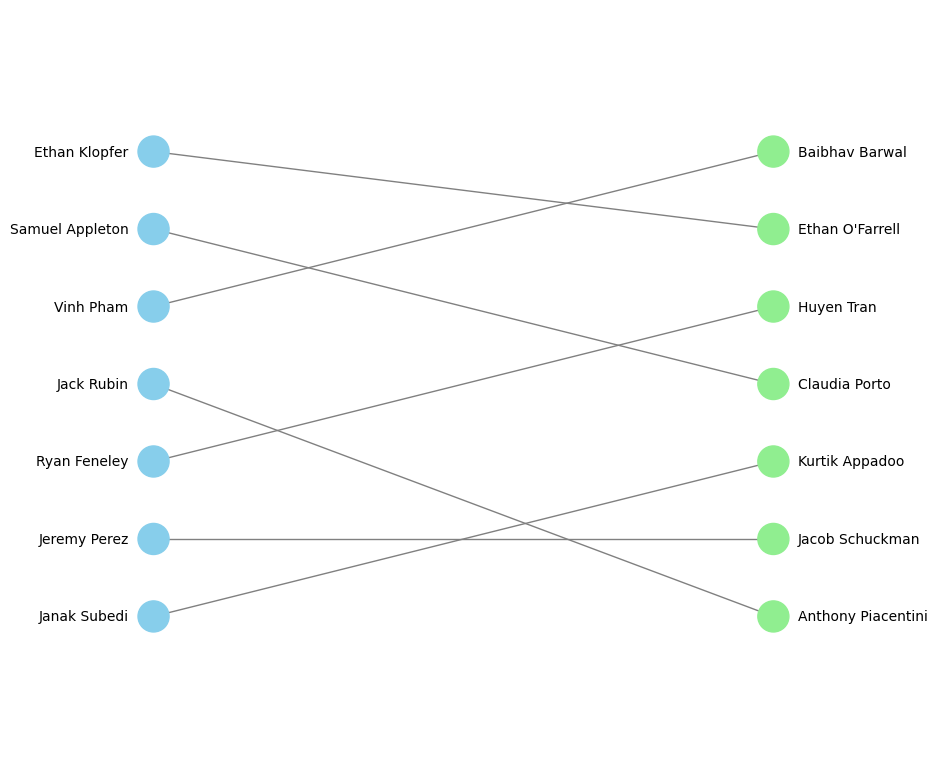
\includegraphics[width=0.75\linewidth]{images/cover.png}} 
\date{\today}

\setcounter{secnumdepth}{3}
\setcounter{tocdepth}{1}

\authorLF{}
\dept{Department of Computer Science}
\advisor{Matthew Anderson}

\begin{document}

\pagenumbering{roman}

\maketitle

\def\changemargin#1#2{\list{}{\rightmargin#2\leftmargin#1}\item[]}
\let\endchangemargin=\endlist 

\begin{changemargin}{0.75in}{0.75in}

\section*{Preface}

This book contains the result of the collective efforts, gathered
knowledge, and engineered algorithms and implementations of the
fourteen students in my Fall 2024 senior project course: CSC-489
\emph{Guided Research in Computer Science}.

The students worked to understand and offer solutions to a
challenging, outstanding open problem in theoretical computer science:
\begin{quote}
\begin{center}
    \emph{How difficult is the Maximum Matching Problem?}
\end{center}
\end{quote}
Each student charted their own path to explore this question.  Some
dove head first into implementation of algorithms.  Some, more
circumspectly, investigate the deep literature on this problem and
computational complexity theory more broadly.  These initial forays
into the wild frontiers of human knowledge, lead to new questions,
techniques, understanding, and connections with other problems.

On its surface this problem seems simple, but as the investigation
deepened they learned that only some cases of the problem are known to
have efficient, polynomial-time algorithms, and some variants are
NP-complete, making it unlikely there will be an efficient algorithm
that can solve it exactly.  This dichotomy lead some students to
investigate the space of efficient algorithms and some to study
related NP-complete problems and ways to solve them.

Some students took paths that I had foreseen into classical matching
algorithms, perfect matching algorithms, stable marriage problems, and
linear and integer programming, but some students delved into rich,
connected topics that I had not, like ant colony optimization,
multi-threading, and real-world applications of matching, like schemes
for organizing kidney donations.

Some of these paths converged quickly, leading to collaborative
efforts, among them developing a testing and evaluation framework for
a problem we do not how to efficiently solve.  Some paths saw students
to take on leadership roles in the research, implementation, and
writing efforts, charting the path for themselves, but also guiding
and supporting their peers.

In the end, all paths taken converge here in this book, which is a
record of the knowledge gained, and our successes and failures in
attempting to answer this vexing question.

I am proud of the work my students accomplished.  It has been a
pleasure watching them grow into mature, professional, reflective,
computer scientists over the last four years---I look forward to
seeing the paths they embark on after Union!

\bigskip

\noindent Schenectady, November 2024 \hfill Matthew Anderson

\end{changemargin}

\newpage
{\small
\tableofcontents}
\newpage

\makepreamble

\pagenumbering{arabic}

\chapter{Introduction}
\label{sec:introduction}
Graph theory provides essential tools for addressing a wide range of complex problems, and one of the most fundamental challenges within this field is the \textbf{Maximum Matching} problem. In its simplest form, this problem asks us to find the largest set of edges in a graph such that no two edges share a vertex. The maximum matching problem has far-reaching applications, including network design, resource allocation, and scheduling. This book is dedicated to understanding the algorithms and techniques that solve this problem, as well as exploring its variations and related concepts in graph theory.



\section{The Maximum Matching Problem}
\label{sec:max_matching}
The \textbf{Maximum Matching Problem} stands as one of the most fundamental challenges in graph theory, with critical relevance to solving complex, real-world problems. Finding a maximum matching extends beyond theoretical interest; it has practical applications in areas such as job assignments, resource allocation, and network connectivity. For example, consider matching a set \( M \) of machines with a set \( T \) of tasks to be performed at the same time. An edge \((u, v) \in E\) means that a machine \( u \in M \) can perform a task \( v \in T \). A maximum matching provides work for as many machines as possible. In this context, an optimal matching ensures that no machine is left idle if there are tasks available, and no task is left incomplete if a machine is capable of performing it. This framework can also be applied to other areas, such as assigning employees to projects or distributing resources efficiently across a network.



The formal definition of the Maximum Matching Problem can be stated as follows:

\begin{center}
    \begin{tabular}{rl} % Right (r) and left (l) alignment
        \textbf{Input}: & Let \(V\) be a set, \(d \geq 2\) be an integer, and \(G = \langle V_d, E \subseteq V_d \rangle\) be a \(d\)-partite graph. \\
        \\
        \textbf{Output}: & \begin{minipage}[t]{0.7\textwidth}
        A maximum matching \(M\) of \(G\), that is, the largest set \(M \subseteq E\) such that for each pair of different edges \(e_1, e_2 \in M\), the vertices in the corresponding positions of \(e_1\) and \(e_2\) in the edges are distinct.
        \end{minipage}
    \end{tabular}
\end{center}

A maximum matching in a graph is defined as a matching that encompasses the largest possible number of edges, ensuring that no other matching can contain more edges than this optimal set \cite{cormen2009introduction}. The largest matching can be at most \( |V| = n \), where \( V \) is the set of vertices in the graph. It is important to note that for all vertices \( v \in V \), at most one edge of \( M \) is incident on \( v \). This property ensures that the matching does not have any duplicate connections, maintaining a one-to-one correspondence between matched vertices. 

To illustrate this concept, consider the bipartite graph depicted in Figure \ref{fig:max_match_bipartite_graph}. In this graph, the vertices are divided into two distinct sets, and edges connect vertices from one set to the other. This straightforward example captures the essence of the maximum matching problem, showcasing the interplay between structure and optimization in graph theory.
\newpage

\begin{figure}[ht]
\centering
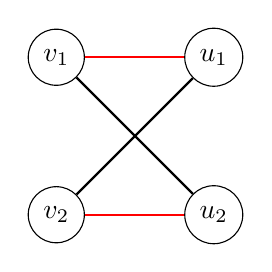
\begin{tikzpicture}[scale=1, transform shape]
    % Nodes
    \node[draw, circle] (v1) at (0,2) {$v_1$};
    \node[draw, circle] (v2) at (0,0) {$v_2$};
    \node[draw, circle] (u1) at (2,2) {$u_1$};
    \node[draw, circle] (u2) at (2,0) {$u_2$};
    
    % Edges
    \draw[red, thick] (v1) -- (u1);   % Matching edge
    \draw[red, thick] (v2) -- (u2);   % Matching edge
    \draw[black, thick] (v1) -- (u2); % Non-matching edge
    \draw[black, thick] (v2) -- (u1); % Non-matching edge
\end{tikzpicture}
\caption{A bipartite graph with maximum matching highlighted in red.}
\label{fig:max_match_bipartite_graph}
\end{figure}


The matching \( M \) for this bipartite graph is defined as:
\[
M = \{ (v_1, u_1), (v_2, u_2) \}
\]



The complexity of the Maximum Matching Problem can vary significantly depending on the type of graph being used. In the case of a \(d\)-partite graph, where the vertex set \(V\) is partitioned into \(d\) subsets, the goal is to find a maximum matching \(M \subseteq E\) such that no two edges in \(M\) share any vertices from the same subset. As \(d\) increases, particularly for \(d \geq 3\), the problem becomes NP-complete, meaning that exact algorithms become infeasible for large instances.

For example, in a hypergraph graph, the challenge lies in effectively navigating the combinations of edges while ensuring distinctness among the vertices involved in the matched pairs. Consider the example shown in Figure \ref{fig:tripartite_graph}.

\begin{figure}[t]
\centering
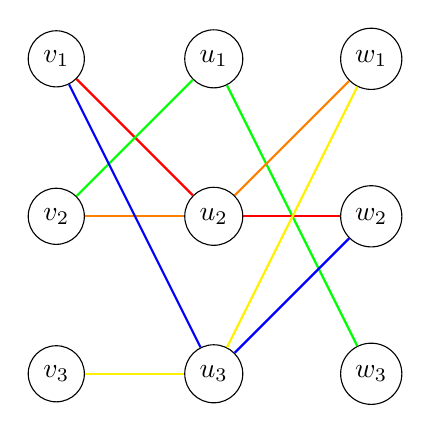
\begin{tikzpicture}[scale=1, transform shape]
    % Nodes
    \node[draw, circle] (v1) at (0,4) {$v_1$};
    \node[draw, circle] (v2) at (0,2) {$v_2$};
    \node[draw, circle] (v3) at (0,0) {$v_3$};
    \node[draw, circle] (u1) at (2,4) {$u_1$};
    \node[draw, circle] (u2) at (2,2) {$u_2$};
    \node[draw, circle] (u3) at (2,0) {$u_3$};
    \node[draw, circle] (w1) at (4,4) {$w_1$};
    \node[draw, circle] (w2) at (4,2) {$w_2$};
    \node[draw, circle] (w3) at (4,0) {$w_3$};
    % Edges
    \draw[red, thick] (v1) -- (u2);   % Matching edge
    \draw[orange, thick] (v2) -- (u2);
    \draw[yellow, thick] (v3) -- (u3); % Matching edge
    \draw[green, thick] (v2) -- (u1);  % Matching edge
    \draw[blue, thick] (v1) -- (u3);   % Non-matching edge
    \draw[green, thick] (u1) -- (w3);  % Non-matching edge
    \draw[orange, thick] (u2) -- (w1); % Matching edge
    \draw[red, thick] (u2) -- (w2);    % Non-matching edge
    \draw[yellow, thick] (u3) -- (w1); % Non-matching edge
    \draw[blue, thick] (u3) -- (w2);   % Non-matching edge
\end{tikzpicture}
\caption{A hypergraph with maximum matching.}
\label{fig:tripartite_graph}
\end{figure}

The maximum matching \( M \) for this tripartite graph is defined as:
\[M = \{ (v_1, u_2, w_2), (v_2, u_1, w_3), (v_3, u_3, w_1) \}\]

This matching connects the vertices across the three sets while ensuring that no two edges share a vertex, thereby maximizing the total number of matched pairs.



The Maximum Matching Problem serves as a critical foundation for understanding complex graph interactions and their applications, providing a gateway into more advanced concepts and algorithms in the realm of graph theory. As mentioned, when \(d \geq 3\), the problem becomes NP-complete, meaning that finding an exact solution is computationally infeasible for large graphs. This motivates the exploration of approximation algorithms and heuristic approaches in practical scenarios.




\section{Organization}
\label{sec:organization}
We begin by establishing the necessary foundations in graph theory, introducing essential concepts like simple graphs, directed versus undirected graphs, adjacency, and subgraphs \ref{sec:graph_theory}. These basic building blocks help form a solid understanding of how graphs are structured and provide the groundwork for more advanced discussions on maximum matching.

As we delve deeper into the topic, we examine various algorithms for maximum matching \ref{sec:existing_algorithms} and their respective runtime complexities. These algorithms are the heart of solving the matching problem, and we explore different approaches depending on the type of graph involved. Bipartite graphs \ref{sec:bipartite_algorithms}, for example, allow for specialized algorithms such as the Edmonds-Karp Algorithm \ref{subsec:edmonds_karp}, while more complex graph structures like d-partite graphs \ref{sec:dpartite_algorithms} require deeper considerations.

The book also covers related problems in graph theory \ref{sec:problem_variants} that have strong connections to maximum matching. Concepts like perfect matching \ref{sec:perfect_matching}, minimum vertex cover \ref{sec:min_vertex_cover}, and maximum flow \ref{sec:max_flow}
play important roles in understanding different matching scenarios. These problems, while distinct, often share underlying principles and solutions that enhance our comprehension of matchings.

In cases where finding exact solutions is computationally expensive, we explore approximation methods and heuristic algorithms \ref{sec:approximation_algorithms}. One such technique is Ant Colony Optimization (ACO) \ref{subsec:aco}, a powerful metaheuristic inspired by natural processes. This method is beneficial for approaching the maximum matching problem in complex and large-scale graphs, where an optimal solution may be too costly to compute.

Finally, we implemented the theory by testing various algorithms through races \ref{sec:testing_evaluation} to determine their efficiency on different graph types. These races helped evaluate performance under varying conditions, such as graph structure and size.

Testing was thorough, using both random and fixed test cases. The use of a visualizer helped verify solutions visually, while automated graph generation streamlined the process. However, automating NP-complete problems like d-partite graph generation posed challenges. Test files followed a consistent format, ensuring reproducibility.

Performance was assessed using metrics such as accuracy, total runtime, and a density-completeness metric. Solvers were evaluated in races based on these criteria, revealing key insights about their strengths and weaknesses. The races showed how algorithms performed in different scenarios, with some excelling in sparse graphs while others struggled with dense configurations. These results highlighted the trade-offs in efficiency and scalability across various solver types.


\chapter{Background}
\label{sec:background}
% Claudia Porto, COMPLETE
In the previous chapter, we were briefly introduced to the maximum matching problem. To fully understand the intricacies of this problem and the multitude of algorithms that can solve it, it is essential to first grasp the underlying concepts in graph theory and computational complexity. By exploring these foundational concepts, we can better understand how to approach the maximum matching problem across different graph types and develop effective algorithms for its solution.

\section{Graph Theory}
\label{sec:graph_theory}
% Claudia Porto, COMPLETE

Graph theory is fundamental in understanding the various graph structures that arise in problems like maximum matching. The structure of the graph significantly influences both the choice of algorithm and its efficiency. By providing essential principles and techniques, graph theory equips us to navigate different graph types and select the most appropriate algorithms for solving matching problems. This understanding is crucial for addressing the challenges posed by diverse graph scenarios and developing efficient, specialized algorithms for maximum matching in various settings.

\subsection{Graphs}
A \textbf{graph} \( G \) is defined as an ordered pair \( G = (V, E) \), where:
\begin{itemize}
    \item \( V \) is an finite set of \textbf{vertices}.
    \item \( E \) is a set of \textbf{edges}, where each edge is an unordered pair of distinct vertices \( u, v \in V \), where \( E \subseteq [V^2]\).
    \begin{itemize}
        \item \([V^2] = V \times V\)
        \item \(V^d = V_1 \times V_2 \times ... \times V_d\)
    \end{itemize}
\end{itemize}
Depending on the context, sometimes graphs are called \textbf{networks}, vertices are called \textbf{nodes}, and edges are called \textbf{arcs}. In a graph, no two edges are identical, between any pair of vertices, there is at most one edge, and there can be \textbf{self loops}, edges of the form \( \{v, v\} \) where a vertex is connected to itself.

For example, consider the graph \( G = (V, E) \) in Figure~\ref{fig:general_graph}:
\[
V = \{1, 2, 3\}, \quad E = \{\{1, 2\}, \{2, 3\}\}
\]

\begin{figure}[h]
\begin{center}
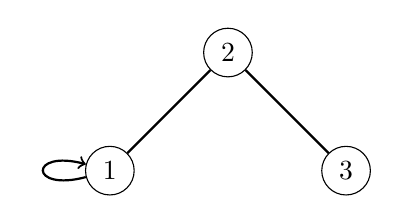
\begin{tikzpicture}[scale=1.5]
    % Draw nodes
    \node[circle, draw] (1) at (0, 0) {1};
    \node[circle, draw] (2) at (1, 1) {2};
    \node[circle, draw] (3) at (2, 0) {3};

    % Draw edges
    \draw[thick] (1) -- (2);
    \draw[thick] (2) -- (3);
    \draw[thick, ->] (1) to[loop left] (1);
\end{tikzpicture}
\caption{A graph with three vertices, two edges, and a self-loop at vertex 1.}
\label{fig:general_graph}
\end{center}
\end{figure}

This represents a graph with three vertices $V = 1, 2, 3$, and two edges connecting vertices 1 and 2, and vertices 2 and 3 with a self loop on vertex 1.\cite{yadav2023advanced, cormen2009introduction}

Graphs can be categorized as either \textbf{undirected} or \textbf{directed}, depending on whether their edges are bidirectional or have a specific direction. 

In an \textbf{undirected graph}, an edge between vertices \( u \) and \( v \) is represented as \( \{u, v\} \), indicating that the edge can be traversed in either direction. An undirected graph is defined as:
\[
G = (V, E) \quad \text{where} \quad E \subseteq \{\{u, v\} \mid u, v \in V, u \neq v \}
\]

In Figure~\ref{fig:undirected_graph}, all edges are bidirectional and can be written as \{\{1,2\}, \{2,3\}, \{1,3\}\} or \{\{2,1\}, \{3,2\}, \{3,1\}\}, among other permutations. All of these are equivalent representations because the order of vertices in an edge does not matter in an undirected graph.

\begin{figure}[h]
\begin{center}
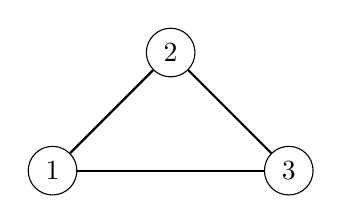
\begin{tikzpicture}[scale=1.5]
    % Draw nodes
    \node[circle, draw] (1) at (0, 0) {1};
    \node[circle, draw] (2) at (1, 1) {2};
    \node[circle, draw] (3) at (2, 0) {3};

    % Draw edges (undirected)
    \draw[thick] (1) -- (2); % Edge between 1 and 2
    \draw[thick] (2) -- (3); % Edge between 2 and 3
    \draw[thick] (1) -- (3); % Edge between 1 and 3
\end{tikzpicture}
\caption{An undirected graph with bidirectional edges connecting vertices 1, 2, and 3.}
\label{fig:undirected_graph}
\end{center}
\end{figure}

In a \textbf{directed graph}, each edge has a specific direction. An edge from vertex \( u \) to vertex \( v \) is denoted by \( (u, v) \), and the edge can only be traversed from \( u \) to \( v \). A directed graph is defined as:
\[
G = (V, E) \quad \text{where} \quad E \subseteq \{(u, v) \mid u, v \in V, u \neq v \}
\]

In this case, \( (u, v) \) is an ordered pair, and the directionality of the edge imposes a one-way relationship from \( u \) to \( v \). For example, consider a directed graph \( G = (V, E) \) in Figure~\ref{fig:directed_graph} where:
\[
V = \{1, 2, 3\}, \quad E = \{(1, 2), (2, 3)\}
\]

\begin{figure}[h]
\begin{center}
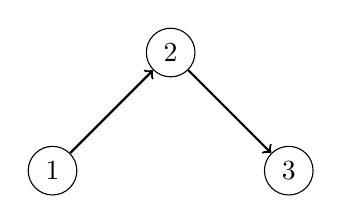
\begin{tikzpicture}[scale=1.5]
    % Draw nodes
    \node[circle, draw] (1) at (0, 0) {1};
    \node[circle, draw] (2) at (1, 1) {2};
    \node[circle, draw] (3) at (2, 0) {3};

    % Draw directed edges
    \draw[thick,->] (1) -- (2); % Directed edge from 1 to 2
    \draw[thick,->] (2) -- (3); % Directed edge from 2 to 3
\end{tikzpicture}
\caption{A directed graph with edges from vertex 1 to 2 and vertex 2 to 3}
\label{fig:directed_graph}
\end{center}
\end{figure}

In this graph, there is a directed edge from vertex 1 to vertex 2, and another directed edge from vertex 2 to vertex 3. \cite{yadav2023advanced, cormen2009introduction}

\subsection{Weighted Graphs}

A \textbf{weighted graph} is a graph in which each edge is assigned an integer, known as the \textbf{weight} of the edge. The weight typically represents a cost, distance, or any measurable attribute of the connection between two vertices.\cite{mathew2017weighted}

Each edge in a weighted graph can be represented by a tuple \((u, v, w)\), where:
\begin{itemize}
    \item \( u \) and \( v \) are vertices connected by the edge.
    \item \( w \) is the weight of the edge between \( u \) and \( v \).
\end{itemize}
Since the graph in this example is undirected, the order of $u$ and $v$ does not matter; the edge \((u,v,w)\) is equivalent to \((v,u,w)\). However, the weight $w$ is always the last part of the tuple and uniquely identifies the value associated with the connection.

For example, consider the weighted graph in Figure~\ref{fig:weighted_graph} where:
\[
V = \{1, 2, 3, 4\}, \quad E = \{(1, 2, 3), (1, 3, 2), (2, 3, 4), (3, 4, 5), (1, 4, 1)\}
\]

\begin{itemize}
    \item The vertices \( V \) represent nodes labeled \( 1 \) through \( 4 \).
    \item The edges \( E \) are tuples that specify the connection between two vertices and their associated weights. For instance, the edge \( (1, 2, 3) \) indicates a connection between vertices \( 1 \) and \( 2 \) with a weight of \( 3 \).
\end{itemize}

Figure~\ref{fig:weighted_graph} visually represents the graph. Each node corresponds to a vertex, and each line connecting two nodes represents an edge labeled with its respective weight. For example:
\begin{itemize}
    \item The edge between vertex \( 1 \) and vertex \( 4 \) has a weight of \( 1 \).
    \item The edge between vertex \( 3 \) and vertex \( 4 \) has a weight of \( 5 \).
\end{itemize} 

\begin{figure}[h]
\begin{center}
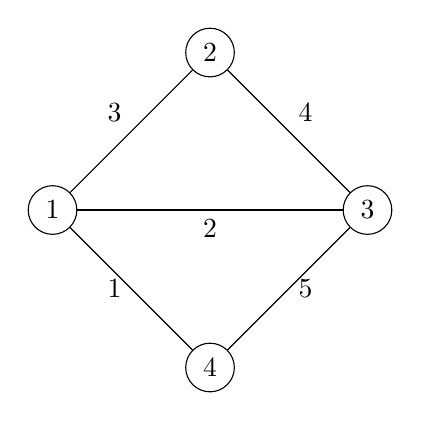
\begin{tikzpicture}
    % Nodes
    \node[draw, circle] (v1) at (0, 0) {1};
    \node[draw, circle] (v2) at (2, 2) {2};
    \node[draw, circle] (v3) at (4, 0) {3};
    \node[draw, circle] (v4) at (2, -2) {4};
  
    % Edges with weights
    \draw[-] (v1) -- node[above left] {3} (v2);
    \draw[-] (v1) -- node[below] {2} (v3);
    \draw[-] (v2) -- node[above right] {4} (v3);
    \draw[-] (v3) -- node[right] {5} (v4);
    \draw[-] (v1) -- node[left] {1} (v4);
\end{tikzpicture}
\caption{A weighted graph with vertices V = 1, 2, 3, 4 and their corresponding weighted edges}
\label{fig:weighted_graph}
\end{center}
\end{figure}

\subsection{Adjacent Vertices and Incident Edges}

Two vertices \( u \) and \( v \) in a graph \( G \) are called \textbf{adjacent} if they are joined by an edge. In an undirected graph, this means \( \{u, v\} \in E(G) \), while in a directed graph, \( u \) is adjacent to \( v \) if \( (u, v) \in E(G) \).

For example, in the undirected graph \( G = (V, E) \) in Figure~\ref{fig:adj_vertices}, where \( V = \{1, 2, 3\} \) and \( E = \{\{1, 2\}, \{2, 3\}\} \), vertices 1 and 2 are adjacent (in red), and vertices 2 and 3 are adjacent (in blue).

\begin{figure}[h]
\begin{center}
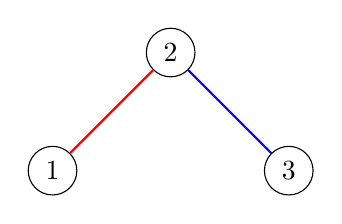
\begin{tikzpicture}[scale=1.5]
    % Draw nodes
    \node[circle, draw] (1) at (0, 0) {1};
    \node[circle, draw] (2) at (1, 1) {2};
    \node[circle, draw] (3) at (2, 0) {3};

    % Draw edges with different colors
    \draw[thick, red] (1) -- (2); % Edge from node 1 to node 2 in red
    \draw[thick, blue] (2) -- (3); % Edge from node 2 to node 3 in blue
\end{tikzpicture}
\caption{An undirected graph showing adjacency between vertices, with edges colored to indicate adjacency relations.}
\label{fig:adj_vertices}
\end{center}
\end{figure}

An edge \( e \) is said to be \textbf{incident} to the vertices it joins. In an undirected graph, if \( e = \{u, v\} \), then \( e \) is incident to both \( u \) and \( v \). In a directed graph, if \( e = (u, v) \), then the edge is incident to \( u \) as an outgoing edge and to \( v \) as an incoming edge.  \cite{yadav2023advanced, cormen2009introduction}

\subsection{Degree of a Vertex}
\vspace{0.05cm}
In an undirected graph, the \textbf{degree} of a vertex \( v \) is the number of edges incident to \( v \), denoted by \( \deg(v) \). \cite{yadav2023advanced, cormen2009introduction} On the other hand, in a directed graph, the degree is split into two parts:
\begin{itemize}
    \item \textbf{In-degree}: The number of edges directed into the vertex \( v \), denoted by \( \deg^-(v) \).
    \item \textbf{Out-degree}: The number of edges directed out of the vertex \( v \), denoted by \( \deg^+(v) \).
\end{itemize}

For example, in the graph \( G = (V, E) \) in Figure~\ref{fig:degree} with \( V = \{1, 2, 3\} \) and \( E = \{\{1, 2\}, \{2, 3\}\} \), the degree of vertex 2 is 2, since it is connected to both vertices 1 and 3.

\begin{figure}[h]
\begin{center}
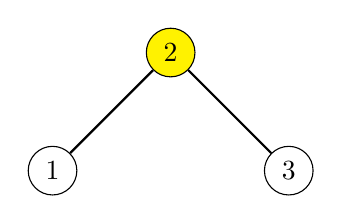
\begin{tikzpicture}[scale=1.5]
    % Draw nodes
    \node[circle, draw] (1) at (0, 0) {1};
    \node[circle, draw, fill=yellow] (2) at (1, 1) {2}; % Highlighted vertex 2 with a fill color
    \node[circle, draw] (3) at (2, 0) {3};

    % Draw edges
    \draw[thick] (1) -- (2);
    \draw[thick] (2) -- (3);
\end{tikzpicture}
\caption{An undirected graph illustrating the degree of vertex 2, highlighted in yellow.}
\label{fig:degree}
\end{center}
\end{figure}

In a directed graph \( G = (V, E) \) in Figure~\ref{fig:directed_degree} with \( V = \{1, 2, 3\} \) and \( E = \{(1, 2), (2, 3)\} \), the in-degree and out-degree of vertex 2 are as follows:
\begin{itemize}
    \item \(\deg^-(2) = 1\) (one edge points into vertex 2)
    \item \(\deg^+(2) = 1\) (one edge points out to vertex 3)
    \item \(\deg^-(1) = 0\)
\end{itemize}

\begin{figure}[h]
\begin{center}
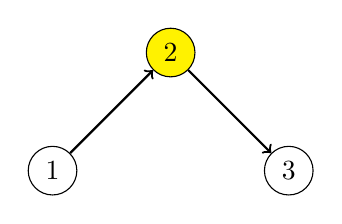
\begin{tikzpicture}[scale=1.5]
    % Draw nodes
    \node[circle, draw] (1) at (0, 0) {1};
    \node[circle, draw, fill=yellow] (2) at (1, 1) {2}; % Highlighted vertex 2 with a fill color
    \node[circle, draw] (3) at (2, 0) {3};

    % Draw directed edges
    \draw[thick,->] (1) -- (2); % Directed edge from 1 to 2
    \draw[thick,->] (2) -- (3); % Directed edge from 2 to 3
\end{tikzpicture}
\caption{A directed graph showing the in-degree and out-degree of vertex 2, highlighted in yellow.}
\label{fig:directed_degree}
\end{center}
\end{figure}

\subsection{Bipartite Graphs}
Let \( V \) be a set of vertices, \( d = 2 \) be an integer, and \( G = (V, E) \) be a bipartite graph. A \textbf{bipartite graph} is a graph where the vertex set \( V \) can be partitioned into two disjoint sets \( V_1 \) and \( V_2 \) such that every edge in \( E \) connects a vertex in \( V_1 \) to a vertex in \( V_2 \). In other words, no two vertices within the same set are adjacent.  \cite{yadav2023advanced}

Formally, \( V = V_1 \cup V_2 \) and \( V_1 \cap V_2 = \emptyset \), with every edge \( e \in E \) satisfying \(e \subseteq V_1 \times V_2\). This means that each edge is a pair \(v_1, v_2\), where \( v_1 \in V_1 \) and \( v_2 \in V_2 \). For example, the following graph in Figure~\ref{fig:bipartite} is bipartite:
\[
V = \{1, 2, 3, 4\}, \quad E = \{\{1, 3\}, \{2,3\}, \{2, 4\}\}
\]

\begin{figure}[h]
\begin{center}
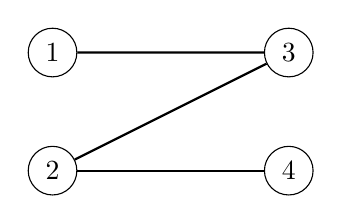
\begin{tikzpicture}[scale=1.5]
    % Draw nodes
    \node[circle, draw] (1) at (0, 1) {1};
    \node[circle, draw] (2) at (0, 0) {2};
    \node[circle, draw] (3) at (2, 1) {3};
    \node[circle, draw] (4) at (2, 0) {4};

    % Draw edges
    \draw[thick] (1) -- (3);
    \draw[thick] (2) -- (3);
    \draw[thick] (2) -- (4);
\end{tikzpicture}
\caption{An example of a bipartite graph}
\label{fig:bipartite}
\end{center}
\end{figure}

In Figure~\ref{fig:bipartite}, \( G = (V, E) \), where \( V = \{1, 2, 3, 4\} \), and the edge set is \( E = \{\{1, 3\}, \{2, 3\}, \{2, 4\}\} \). This graph satisfies the condition that every edge connects a vertex from \( V_1 \) to a vertex from \( V_2 \), and no edge connects two vertices within the same set.

\subsection{Hypergraphs}
A \textbf{hypergraph} \( H = (V, E) \) is a generalization of a graph, where \( V \) is the set of vertices and \( E \) is the set of \textbf{hyperedges}. Unlike in traditional graphs, where each edge connects exactly two vertices, a hyperedge in a hypergraph can connect any number of vertices. More formally, each hyperedge is a subset of \( V \), which may contain more than two elements \cite{cormen2009introduction}.

For example, consider a hypergraph \( H = (V, E) \) in Figure~\ref{fig:hypergraph} where:
\[
V = \{1, 2, 3, 4\}, \quad E = \{\{1, 2\}, \{2, 3, 4\}\}
\]
Here, the hyperedge \( \{1, 2\} \) connects vertices 1 and 2, and the hyperedge \( \{2, 3, 4\} \) connects vertices 2, 3, and 4. The key distinction from traditional graphs is that a hyperedge can contain more than two vertices, as seen with \( \{2, 3, 4\} \), which connects three vertices simultaneously. This capability enables hypergraphs to model more intricate relationships, such as multi-way interactions, which cannot be easily captured by standard graphs.

\begin{figure}[h]
\begin{center}
\begin{tikzpicture}
    % Draw nodes
    \node (v1) at (0,0) [draw, circle, inner sep=2pt] {$1$};
    \node (v2) at (1.5,2) [draw, circle, inner sep=2pt] {$2$};
    \node (v3) at (3,0) [draw, circle, inner sep=2pt] {$3$};
    \node (v4) at (3,2) [draw, circle, inner sep=2pt] {$4$};

    % Hyperedges
    \begin{scope}[fill opacity=0.5]
    % Hyperedge connecting 2, 3, and 4
    \filldraw[fill=yellow!70] 
        ($(v2)+(-0.5,0)$) 
        to[out=90,in=180] ($(v4) + (1,0.5)$) 
        to[out=0,in=90] ($(v3) + (0,-1)$)
        to[out=270,in=0] ($(v4) + (0,-3)$)
        to[out=180,in=270] ($(v2)+(-0.5,0)$);
    
    % Hyperedge connecting 1 and 2
    \filldraw[fill=blue!70] 
        ($(v1)+(-0.5,-0.2)$) 
        to[out=90,in=180] ($(v2) + (0.5,0.5)$) 
        to[out=0,in=90] ($(v1)+(0.4,-0.2)$)
        to[out=270,in=0] ($(v1)+(-0.5,-0.2)$);
    \end{scope}

    % Labels for hyperedges
    \node at (2, 3) {$e_2 = \{2, 3, 4\}$};
    \node at (0, -1) {$e_1 = \{1, 2\}$};
\end{tikzpicture}
\caption{An example of a hypergraph}
\label{fig:hypergraph}
\end{center}
\end{figure}

Hypergraphs are particularly useful in problems that involve complex sets and relationships, such as:
\begin{itemize}
    \item \textbf{3D Matching}: In this problem, the goal is to find a matching between sets of vertices, where each matching involves three vertices rather than two, naturally fitting the framework of hypergraphs.
    \item \textbf{Set Cover}: Hypergraphs can be used to represent set cover problems, where each hyperedge corresponds to a set, and the goal is to cover the entire vertex set using the fewest number of hyperedges.
\end{itemize}

In contrast to traditional graphs, where edges simply represent pairwise connections, hypergraphs can represent more general relationships between sets of vertices, making them a powerful tool in the study of combinatorial structures and optimization problems.

\subsection{D-Partite Graphs} 
Let \( V \) be a set, \( d \geq 2 \) be an integer, and \( G = (V, E) \) be a d-partite graph, where \(V = V_1 \cup V_2 ... \cup V_d\) and \(E \subseteq V_1 \times V_2 \times ... \times V_d\). A \textbf{d-partite graph} \( G = (V, E) \) is a type of hypergraph where the vertex set \( V \) can be partitioned into \( d \) disjoint sets \( V_1, V_2, \dots, V_d \) such that no two vertices within the same set are adjacent. Edges have exactly one vertex from each set. For example, consider the 3-partite graph in Figure~\ref{fig:d-partite}:
\[
V = \{1, 2, 3, 4, 5, 6\}, \quad E = \{\{1, 3, 6\}, \{2, 4, 5\}\}
\]

The edges connect vertices between different partitions.
\[
V_1 = \{1, 2\}, \quad V_2 = \{3, 4\}, \quad V_3 = \{5, 6\}
\]

\begin{figure}[h]
\begin{center}
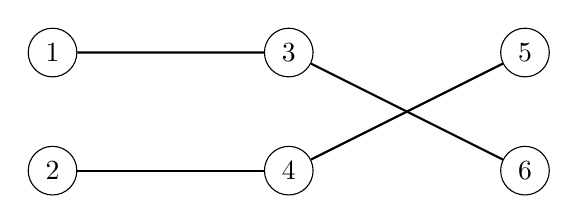
\begin{tikzpicture}[scale=1.5]
    % Draw nodes for V_1
    \node[circle, draw] (1) at (0, 1) {1};
    \node[circle, draw] (2) at (0, 0) {2};

    % Draw nodes for V_2
    \node[circle, draw] (3) at (2, 1) {3};
    \node[circle, draw] (4) at (2, 0) {4};

    % Draw nodes for V_3
    \node[circle, draw] (5) at (4, 1) {5};
    \node[circle, draw] (6) at (4, 0) {6};

    % Draw edges
    \draw[thick] (1) -- (3);
    \draw[thick] (2) -- (4);
    \draw[thick] (4) -- (5);
    \draw[thick] (3) -- (6);
\end{tikzpicture}
\caption{An example of a 3-partite graph}
\label{fig:d-partite}
\end{center}
\end{figure}

D-partite graphs are commonly seen in multi-dimensional matching problems, and algorithms for these graphs extend ideas from bipartite matching to higher dimensions.

\subsection{Matching}
A \textbf{matching} in a graph \( G = (V, E) \) is a subset \( M \subseteq E \) such that no two edges in \( M \) share a common vertex. In other words, a matching is a collection of edges where each vertex is incident to at most one edge.\cite{yadav2023advanced} For example, consider the following bipartite graph:
\[
V = \{1, 2, 3, 4, 5, 6\}, \quad E = \{\{1, 4\}, \{1, 5\}, \{2, 4\}, \{2, 6\}, \{3, 5\}, \{3, 6\}\}
\]

\begin{figure}[h]
\begin{center}
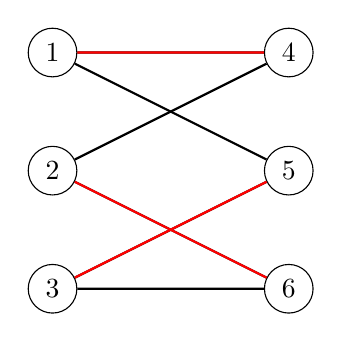
\begin{tikzpicture}[scale=1.5]
    % Draw nodes for set U
    \node[circle, draw] (u1) at (0, 1) {1};
    \node[circle, draw] (u2) at (0, 0) {2};
    \node[circle, draw] (u3) at (0, -1) {3};

    % Draw nodes for set V
    \node[circle, draw] (v1) at (2, 1) {4};
    \node[circle, draw] (v2) at (2, 0) {5};
    \node[circle, draw] (v3) at (2, -1) {6};

    % Draw all edges (undirected)
    \draw[thick] (u1) -- (v1); % Edge between 1 and 4
    \draw[thick] (u1) -- (v2); % Edge between 1 and 5
    \draw[thick] (u2) -- (v1); % Edge between 2 and 4
    \draw[thick] (u2) -- (v3); % Edge between 2 and 6
    \draw[thick] (u3) -- (v2); % Edge between 3 and 5
    \draw[thick] (u3) -- (v3); % Edge between 3 and 6

    % Highlight the matching edges
    \draw[thick, red] (u1) -- (v1); % Highlight matching edge between 1 and 4
    \draw[thick, red] (u2) -- (v3); % Highlight matching edge between 2 and 6
    \draw[thick, red] (u3) -- (v2); % Highlight matching edge between 3 and 5
\end{tikzpicture}
\caption{An example of a matching in a bipartite graph. The highlighted edges form a matching.}
\label{fig:matching}
\end{center}
\end{figure}

A valid matching is \( M = \{\{1, 4\}, \{2, 6\}, \{3, 5\}\} \).

Now consider the following 3-partite graph in Figure~\ref{fig:matching_d3}:
\[
V_1 = \{1, 2, 3\}, \quad V_2 = \{4, 5, 6\}, \quad V_3 = \{7, 8, 9\}
\]
\[
E = \{\{1, 4, 7\}, \{1, 5, 8\}, \{2, 5, 9\}, \{2, 6, 7\}, \{3, 6, 8\}, \{3, 7, 9\}\}
\]

\begin{figure}[h]
\begin{center}
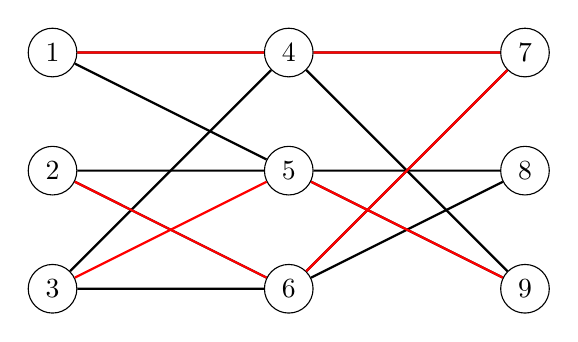
\begin{tikzpicture}[scale=1.5]
    % Draw nodes for set V1
    \node[circle, draw] (v11) at (0, 2) {1};
    \node[circle, draw] (v12) at (0, 1) {2};
    \node[circle, draw] (v13) at (0, 0) {3};

    % Draw nodes for set V2
    \node[circle, draw] (v21) at (2, 2) {4};
    \node[circle, draw] (v22) at (2, 1) {5};
    \node[circle, draw] (v23) at (2, 0) {6};

    % Draw nodes for set V3
    \node[circle, draw] (v31) at (4, 2) {7};
    \node[circle, draw] (v32) at (4, 1) {8};
    \node[circle, draw] (v33) at (4, 0) {9};

    % Draw edges between sets V1, V2, and V3
    \draw[thick] (v11) -- (v21) -- (v31); % Edge between 1, 4, and 7
    \draw[thick] (v11) -- (v22) -- (v32); % Edge between 1, 5, and 8
    \draw[thick] (v12) -- (v22) -- (v33); % Edge between 2, 5, and 9
    \draw[thick] (v12) -- (v23) -- (v31); % Edge between 2, 6, and 7
    \draw[thick] (v13) -- (v23) -- (v32); % Edge between 3, 6, and 8
    \draw[thick] (v13) -- (v21) -- (v33); % Edge between 3, 7, and 9

    % Highlight the matching edges
    \draw[thick, red] (v11) -- (v21) -- (v31); % Highlight matching edge between 1, 4, and 7
    \draw[thick, red] (v12) -- (v23) -- (v31); % Highlight matching edge between 2, 6, and 7
    \draw[thick, red] (v13) -- (v22) -- (v33); % Highlight matching edge between 3, 5, and 9
\end{tikzpicture}
\caption{An example of a matching in a 3-partite graph. The highlighted edges form a matching.}
\label{fig:matching_d3}
\end{center}
\end{figure}

A valid matching is \( M = \{\{1, 4, 7\}, \{2, 6, 7\}, \{3, 5, 8\}\} \).

\subsection{Paths, Cycles, and Augmenting Paths}

A \textbf{path} in a graph \( G = (V, E) \) is a sequence of vertices \( v_1, v_2, \dots, v_k \) such that for each \( i = 1, 2, \dots, k-1 \), the edge \( \{v_i, v_{i+1}\} \in E \). In directed graphs, the edges must be oriented in the direction of traversal. For example in Figure~\ref{fig:path}, in an undirected graph with vertices \( V = \{1, 2, 3, 4\} \) and edges \( E = \{\{1, 2\}, \{2, 3\}, \{3, 4\}\} \), the sequence \( 1, 2, 3, 4 \) forms a path. \cite{yadav2023advanced, cormen2009introduction}

\begin{figure}[h]
\begin{center}
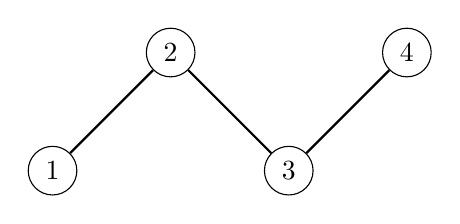
\begin{tikzpicture}[scale=1.5]
    % Draw nodes
    \node[circle, draw] (1) at (0, 0) {1};
    \node[circle, draw] (2) at (1, 1) {2};
    \node[circle, draw] (3) at (2, 0) {3};
    \node[circle, draw] (4) at (3, 1) {4};

    % Draw edges
    \draw[thick] (1) -- (2);
    \draw[thick] (2) -- (3);
    \draw[thick] (3) -- (4);
\end{tikzpicture}
\caption{Undirected Path in a Graph}
\label{fig:path}
\end{center}
\end{figure}

In a directed graph, the edges must be oriented. For example in Figure~\ref{fig:directed_path}, in a directed graph with vertices \( V = \{1, 2, 3, 4\} \) and edges \( E = \{(1, 2), (2, 3), (3, 4)\} \), the sequence \( 1 \to 2 \to 3 \to 4 \) forms a path.

\begin{figure}[h]
\begin{center}
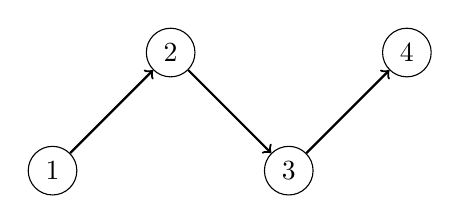
\begin{tikzpicture}[scale=1.5]
    % Draw nodes
    \node[circle, draw] (1) at (0, 0) {1};
    \node[circle, draw] (2) at (1, 1) {2};
    \node[circle, draw] (3) at (2, 0) {3};
    \node[circle, draw] (4) at (3, 1) {4};

    % Draw directed edges
    \draw[thick,->] (1) -- (2);
    \draw[thick,->] (2) -- (3);
    \draw[thick,->] (3) -- (4);
\end{tikzpicture}
\caption{Directed Path in a Graph}
\label{fig:directed_path}
\end{center}
\end{figure}

A \textbf{cycle} is a path that starts and ends at the same vertex. Formally, a cycle is a path \( v_1, v_2, \dots, v_k, v_1 \), where \( k \geq 3 \) and all the edges \( \{v_i, v_{i+1}\} \) for \( i = 1, 2, \dots, k-1 \), as well as \( \{v_k, v_1\} \), belong to \( E(G) \). For example in Figure~\ref{fig:cycle}, in an undirected graph with vertices \( V = \{1, 2, 3\} \) and edges \( E = \{\{1, 2\}, \{2, 3\}, \{3, 1\}\} \), the sequence \( 1, 2, 3, 1 \) forms a cycle. \cite{yadav2023advanced, cormen2009introduction}

\begin{figure}[h]
\begin{center}
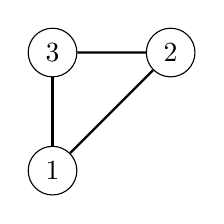
\begin{tikzpicture}[scale=1.5]
    % Draw nodes
    \node[circle, draw] (1) at (0, 0) {1};
    \node[circle, draw] (2) at (1, 1) {2};
    \node[circle, draw] (3) at (0, 1) {3};

    % Draw edges
    \draw[thick] (1) -- (2);
    \draw[thick] (2) -- (3);
    \draw[thick] (3) -- (1);
\end{tikzpicture}
\caption{Undirected Cycle in a Graph}
\label{fig:cycle}
\end{center}
\end{figure}

In a directed graph, a cycle can also be formed. For example in Figure~\ref{fig:directed_cycle}, in a directed graph with vertices \( V = \{1, 2, 3\} \) and edges \( E = \{(1, 2), (2, 3), (3, 1)\} \), the sequence \( 1 \to 2 \to 3 \to 1 \) forms a directed cycle.

\begin{figure}[h]
\begin{center}
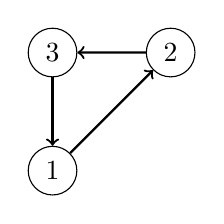
\begin{tikzpicture}[scale=1.5]
    % Draw nodes
    \node[circle, draw] (1) at (0, 0) {1};
    \node[circle, draw] (2) at (1, 1) {2};
    \node[circle, draw] (3) at (0, 1) {3};

    % Draw directed edges
    \draw[thick,->] (1) -- (2);
    \draw[thick,->] (2) -- (3);
    \draw[thick,->] (3) -- (1);
\end{tikzpicture}
\caption{Directed Cycle in a Graph}
\label{fig:directed_cycle}
\end{center}
\end{figure}

Let $G$ be a graph, and $M$ be a matching of $G$, then an \textbf{augmenting path} in $G$ alternates between edges in $M$ and edges that are not, beginning and ending at unmatched vertices.\cite{cormen2009introduction} For example in Figure~\ref{fig:augmenting_path}, consider a bipartite graph with vertex sets: 
\[ V = \{1, 2, 3, 4, 5, 6\}, \quad V_1 = \{1, 2, 3\}, \quad V_2 = \{4, 5, 6\}, \quad E = \{\{1, 4\}, \{2, 4\}, \{2, 5\}, \{3, 5\}, \{3, 6\}\} \] 

For the matching \( M = \{\{2, 4\}, \{3, 5\}\} \), the path \( 1 \to 4 \textcolor{red}{ \to} 2 \to 5 \textcolor{red}{ \to} 3 \to 6 \) forms an augmenting path because it starts at unmatched vertex 1, ends at unmatched vertex 6, and alternates between edges that are matched and unmatched. The red highlights indicate a matched edge.

\begin{figure}[h]
\begin{center}
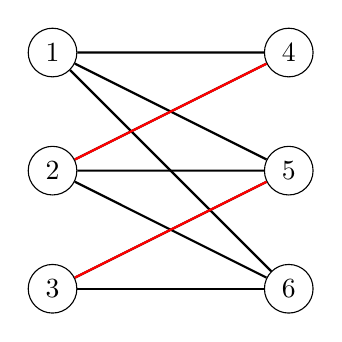
\begin{tikzpicture}[scale=1.5]
    % Draw nodes for V_1
    \node[circle, draw] (1) at (0, 2) {1};
    \node[circle, draw] (2) at (0, 1) {2};
    \node[circle, draw] (3) at (0, 0) {3};

    % Draw nodes for V_2
    \node[circle, draw] (4) at (2, 2) {4};
    \node[circle, draw] (5) at (2, 1) {5};
    \node[circle, draw] (6) at (2, 0) {6};

    % Draw edges
    \draw[thick] (1) -- (4);
    \draw[thick] (2) -- (4);
    \draw[thick] (2) -- (5);
    \draw[thick] (3) -- (5);
    \draw[thick] (3) -- (6);
    \draw[thick] (1) -- (5);
    \draw[thick] (2) -- (6);
    \draw[thick] (1) -- (6);

    % Draw matching edge (thicker and in red)
    \draw[thick, red] (2) -- (4);
    \draw[thick, red] (3) -- (5);
\end{tikzpicture}
\caption{Augmenting Path in a Bipartite Graph}
\label{fig:augmenting_path}
\end{center}
\end{figure}

\subsection{Connected Graphs}
A graph \( G = (V, E) \) is said to be \textbf{connected} if for every pair of vertices \( u, v \in V \), there exists a path from \( u \) to \( v \). In other words, all vertices in the graph are reachable from any other vertex \cite{yadav2023advanced, cormen2009introduction}.

If a graph is not connected, it is called \textbf{disconnected}. A disconnected graph consists of multiple \textbf{connected components}. A \textbf{connected component} of a graph is a maximal subgraph in which every pair of vertices is connected by a path. In other words, a connected component is a subset of the graph where there is a path between every pair of vertices, and no additional vertices or edges from outside the subset can be added without losing its connectivity.

For example, consider the graph \( G = (V, E) \) where:
\[
V = \{1, 2, 3, 4, 5\}, \quad E = \{\{1, 2\}, \{2, 3\}, \{4, 5\}\}
\]
The graph in Figure~\ref{fig:connected_graph} is disconnected, as there is no path between vertex 3 and vertex 4. This graph can be divided into two connected components:
\begin{itemize}
    \item Component 1: The vertices \( \{1, 2, 3\} \) with edges \( \{1, 2\}, \{2, 3\} \).
    \item Component 2: The vertices \( \{4, 5\} \) with edge \( \{4, 5\} \).
\end{itemize}

\begin{figure}[h]
\begin{center}
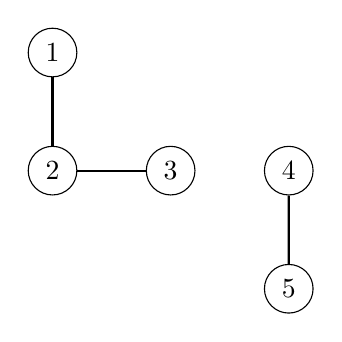
\begin{tikzpicture}[scale=1.5]
    % Draw nodes for the first connected component
    \node[circle, draw] (1) at (0, 1) {1};
    \node[circle, draw] (2) at (0, 0) {2};
    \node[circle, draw] (3) at (1, 0) {3};

    % Draw edges for the first connected component
    \draw[thick] (1) -- (2);
    \draw[thick] (2) -- (3);

    % Draw nodes for the second connected component
    \node[circle, draw] (4) at (2, 0) {4};
    \node[circle, draw] (5) at (2, -1) {5};

    % Draw edges for the second connected component
    \draw[thick] (4) -- (5);
\end{tikzpicture}
\caption{An example of a disconnected graph with two connected components.}
\label{fig:connected_graph}
\end{center}
\end{figure}

\subsection{Complete Graphs}
A \textbf{complete graph} \( K_n \) is a graph where every pair of distinct vertices is connected by an edge. Formally, a complete graph with \( n \) vertices has \( \frac{n(n-1)}{2} \) edges, as all possible pairs of vertices are connected. For example, the complete graph \( K_3 \) in Figure~\ref{fig:complete_graph} has the following edges:
\[
V = \{1, 2, 3\}, \quad E = \{\{1, 2\}, \{1, 3\}, \{2, 3\}\}
\]
This results in 3 edges, which is the maximum number of edges in a graph with 3 vertices.

\begin{figure}[h]
\begin{center}
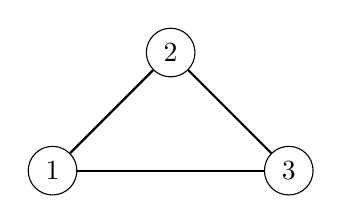
\begin{tikzpicture}[scale=1.5]
    % Draw nodes
    \node[circle, draw] (1) at (0, 0) {1};
    \node[circle, draw] (2) at (1, 1) {2};
    \node[circle, draw] (3) at (2, 0) {3};

    % Draw edges (undirected)
    \draw[thick] (1) -- (2); % Edge between 1 and 2
    \draw[thick] (2) -- (3); % Edge between 2 and 3
    \draw[thick] (1) -- (3); % Edge between 1 and 3
\end{tikzpicture}
\caption{An example of the complete graph \( K_3 \), where every pair of distinct vertices is connected by an edge.}
\label{fig:complete_graph}
\end{center}
\end{figure}

Complete graphs are often used in theoretical explorations of matching, covering, and flow problems, as they provide the maximum number of potential connections between vertices \cite{yadav2023advanced, cormen2009introduction}.

\subsubsection*{Complete \( d \)-Partite Graphs}

A \textbf{complete \( d \)-partite graph} is a graph where the vertex set \( V \) is partitioned into \( d \) disjoint sets \( V_1, V_2, \dots, V_d \), and every vertex in one set is connected to every vertex in the other sets, but there are no edges between vertices within the same set.

For \( d = 2 \), this is simply a \textbf{complete bipartite graph}, where the vertex set \( V \) is divided into two disjoint sets \( V_1 \) and \( V_2 \), and every vertex in \( V_1 \) is connected to every vertex in \( V_2 \), but there are no edges between vertices within \( V_1 \) or within \( V_2 \). A complete bipartite graph is denoted as \( K_{m,n} \), where \( m \) and \( n \) are the sizes of the two disjoint sets \( V_1 \) and \( V_2 \), respectively. The number of edges in \( K_{m,n} \) is given by \( m \times n \).

For example in Figure~\ref{fig:complete_bipartite}, consider the complete bipartite graph \( K_{3,3} \), where:
\[
V_1 = \{1, 2, 3\}, \quad V_2 = \{4, 5, 6\}, \quad E = \{\{1,4\}, \{1,5\}, \{1,6\}, \{2,4\}, \{2,5\}, \{2,6\}, \{3,4\}, \{3,5\}, \{3,6\}\}.
\]

\begin{figure}[h]
\begin{center}
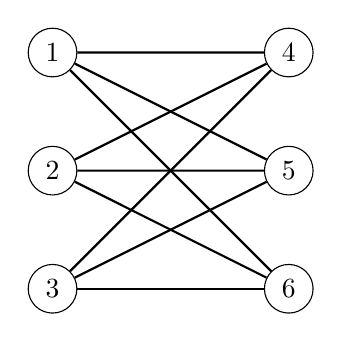
\begin{tikzpicture}[scale=1.5, every node/.style={circle, draw}]
    % Nodes for the first partition
    \node (1) at (0, 2) {1};
    \node (2) at (0, 1) {2};
    \node (3) at (0, 0) {3};
    
    % Nodes for the second partition
    \node (4) at (2, 2) {4};
    \node (5) at (2, 1) {5};
    \node (6) at (2, 0) {6};
    
    % Edges between the two partitions
    \draw[thick] (1) -- (4);
    \draw[thick] (1) -- (5);
    \draw[thick] (1) -- (6);
    \draw[thick] (2) -- (4);
    \draw[thick] (2) -- (5);
    \draw[thick] (2) -- (6);
    \draw[thick] (3) -- (4);
    \draw[thick] (3) -- (5);
    \draw[thick] (3) -- (6);
\end{tikzpicture}
\caption{A complete bipartite graph \( K_{3,3} \) with two partitions \( V_1 = \{1, 2, 3\} \) and \( V_2 = \{4, 5, 6\} \). Every vertex in \( V_1 \) is connected to every vertex in \( V_2 \).}
\label{fig:complete_bipartite}
\end{center}
\end{figure}

For \( d > 2 \), the complete \( d \)-partite graph consists of \( d \) disjoint vertex sets \( V_1, V_2, \dots, V_d \), and every vertex in \( V_i \) is connected to every vertex in all other sets \( V_j \) (for \( i \neq j \)), but there are no edges between vertices within the same set. The number of edges in a complete \( d \)-partite graph is the sum of the edges between each pair of sets, calculated as:
\[
\text{Total edges} = \sum_{1 \leq i < j \leq d} |V_i| \times |V_j|
\]
This formula counts the edges between each pair of disjoint sets.

\subsection{Graph Representations}
A graph \( G = (V, E) \) can be represented as an adjacency matrix or as a collection of adjacency lists. If a graph is dense (\(|E|\) is close to \(|V|^2\)), an adjacency matrix is used. If a graph is sparse (\(|E|\) is much less than \(|V|^2\)), an adjacency list is the more efficient choice. \cite{yadav2023advanced} \cite{cormen2009introduction}

\subsubsection*{Adjacency Matrix}
The \textbf{adjacency matrix} of a bipartite graph \( G = (V, E) \) with two sets of vertices is an \( n \times m \) matrix \( A \) where each entry \( A_{ij} \) is defined as follows:
\[
A_{ij} =
\begin{cases}
1, & \text{if } \{u_i, v_j\} \in E, and \\
0, & \text{otherwise}
\end{cases}
\]
For example, consider the bipartite graph \( G = (V, E) \) where:
\[
V_1 = \{1, 2\}, \quad V_2 = \{3, 4\}, \quad E = \{\{1, 3\}, \{1, 4\}, \{2, 4\}\}
\]
The adjacency matrix \( A \) for this bipartite graph is:
\[
A =
\begin{bmatrix}
1 & 1 \\
0 & 1 
\end{bmatrix}
\]
where rows correspond to vertices in \( V_1 \) and columns correspond to vertices in \( V_2 \).

\begin{figure}[h]
\begin{center}
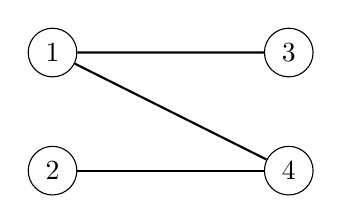
\begin{tikzpicture}[scale=1.5]
    % Draw nodes for V1
    \node[circle, draw] (1) at (0, 1) {1};
    \node[circle, draw] (2) at (0, 0) {2};

    % Draw nodes for V2
    \node[circle, draw] (3) at (2, 1) {3};
    \node[circle, draw] (4) at (2, 0) {4};

    % Draw edges
    \draw[thick] (1) -- (3);
    \draw[thick] (1) -- (4);
    \draw[thick] (2) -- (4);
\end{tikzpicture}
\caption{Adjacency Matrix Representation of a Bipartite Graph}
\label{fig:adj_matrix}
\end{center}
\end{figure}

Adjacency matrices are used to quickly tell if there is an edge connecting two given vertices. The adjacency matrix is particularly useful in algorithms where matrix multiplication or graph traversal plays a significant role, such as in finding augmenting paths for matchings. The amount of memory required is $\Theta(V^2)$, which is independent of the number of edges on the graph.

\subsubsection*{Adjacency List}
The \textbf{adjacency list} of a bipartite graph \( G = (V, E) \) is a collection of lists, one for each vertex, where each list contains the vertices adjacent to that vertex.

For example, consider the bipartite graph \( G = (V, E) \) where:
\[
V_1 = \{1, 2\}, \quad V_2 = \{3, 4\}, \quad E = \{\{1, 3\}, \{1, 4\}, \{2, 4\}\}
\]
The adjacency list for the following bipartite graph is:
\[
\text{Adjacency List:}
\begin{array}{l}
1: \{3, 4\} \\
2: \{4\} \\
3: \{1\} \\
4: \{1, 2\}
\end{array}
\]

\begin{figure}[h]
\begin{center}
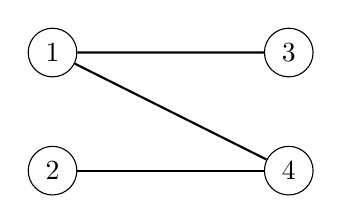
\begin{tikzpicture}[scale=1.5]
    % Draw nodes for V1
    \node[circle, draw] (1) at (0, 1) {1};
    \node[circle, draw] (2) at (0, 0) {2};

    % Draw nodes for V2
    \node[circle, draw] (3) at (2, 1) {3};
    \node[circle, draw] (4) at (2, 0) {4};

    % Draw edges
    \draw[thick] (1) -- (3);
    \draw[thick] (1) -- (4);
    \draw[thick] (2) -- (4);
\end{tikzpicture}
\caption{Adjacency List Representation of a Bipartite Graph}
\label{fig:adj_list}
\end{center}
\end{figure}

This representation is efficient for sparse graphs and is widely used in graph traversal algorithms. For example, finding an augmenting path in matching algorithms can be performed efficiently using adjacency lists. The amount of memory required is $\Theta(V+E)$.

\subsection{Berge's Theorem}
It is not \textit{a priori} easy to determine whether a given matching is maximum; the obvious way to do so involves searching for all other matchings.
Berge's theorem gives an easier method for general graphs:

\begin{theorem}\label{berge} \cite{berge}
    A matching $M$ in a graph $G$ is a maximum matching if and only if has no augmenting path.
\end{theorem}

Consider the matching $\{(2, 4), (3, 5)\}$ in the following graph. It is not maximum; it has the augmenting path (1,4), (4, 2), (2, 5), (5, 3), (3, 6).

\begin{center}
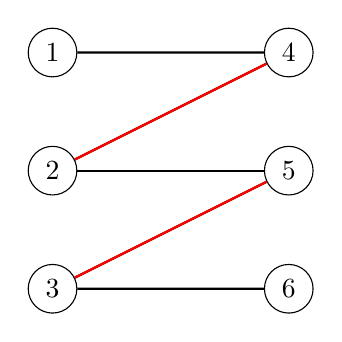
\begin{tikzpicture}[scale=1.5]
    % Draw nodes for set U
    \node[circle, draw] (u1) at (0, 1) {1};
    \node[circle, draw] (u2) at (0, 0) {2};
    \node[circle, draw] (u3) at (0, -1) {3};

    % Draw nodes for set V
    \node[circle, draw] (v1) at (2, 1) {4};
    \node[circle, draw] (v2) at (2, 0) {5};
    \node[circle, draw] (v3) at (2, -1) {6};

    % Draw all edges (undirected)
    \draw[thick] (u1) -- (v1); % Edge between 1 and 4
    \draw[thick] (u2) -- (v1); % Edge between 2 and 4
    \draw[thick] (u2) -- (v2); % Edge between 2 and 5
    \draw[thick] (u3) -- (v2); % Edge between 3 and 5
    \draw[thick] (u3) -- (v3); % Edge between 3 and 6

    % Highlight the matching edges
    \draw[thick, red] (u2) -- (v1); % Highlight matching edge between 2 and 4
    \draw[thick, red] (u3) -- (v2); % Highlight matching edge between 3 and 5
\end{tikzpicture}
\label{fig:berge_example}
\end{center}

\begin{proof}[Proof of \Cref{berge}]
Suppose $M$ has an augmenting path $P$ and let us prove $M$ is not maximum. It may be assumed that $P$ is simple.
We claim the symmetric difference $(M - P) \cup (P - M)$ is a matching.
For example, suppose $e$ and $e'$ are distinct edges of $(M - P) \cup (P - M)$ sharing a vertex. 

There are three cases:
(1) Both are in $M$: We reach a contradiction since $M$ is a matching.

(2) Both are in $P - M$: then $e$ and $e'$ are successive edges since $P$ is simple.
As $P$ is augmenting, one of $e, e'$ is in $M$, a contradiction.

(3) One (say $e$) is in $M - P$ and the other (say $e'$) is in $P - M$.
Let $v$ be the vertex shared by $e$ and $e'$.
Since $e \in M$ and $P$ is augmenting, $v$ is not an endpoint of $P$.
So there is another edge $e'' \in P$ that also contains $v$.
Observe that $e$ and $e''$ are distinct vertices of $M$ containing $v$ for a contradiction.

Also, $|(M - P) \cup (P - M)| = (|M| - \frac{|P| - 1}{2}) + \frac{|P| + 1}{2} = |M| + 1$ to conclude.

In the other direction,  suppose $M$ has no augmenting path.
To show that $M$ is maximum, let $M'$ be another matching of $G$.
Consider the symmetric difference graph $(M - M')\cup (M' - M)$.
The connected components of $(M - M')\cup (M' - M)$ are simple paths and even cycles alternating between edges in $M$ and $M'$. The assumption on $M$ ensures each of the former start or end with an edge of $M$ (for otherwise they would be an augmenting path for $M$).
Thus each component has intersection with $M$ at least as large as with $M'$, showing $|M| - |M\cap M'| = |M - M'| \geq |M' - M| = |M'| - |M\cap M'|$ i.e. $|M| \geq |M'|$.
\end{proof}

The proof of Theorem \Cref{berge} gives a strategy to find a maximum matching: beginning with a matching (such as $\varnothing$), repeatedly finding augmenting paths and taking symmetric differences until there are no more.
This strategy is key to various algorithms in Chapter 4.

\section{P vs. NP}
\label{sec:P_vs_NP}
\textbf{ Polynomial Time}, also known as P, refers to the class of decision problems that can be solved efficiently by a deterministic algorithm in polynomial time. A problem is in P if there exists an algorithm that can find a solution in a time complexity that is at most a polynomial function of the size of the input\cite{cormen2009}. In practical terms, this means that as the input size grows, the time required to solve the problem increases at a manageable rate, which allows for efficient computation.

Examples of problems in P include common computational tasks such as sorting a list of numbers (using algorithms like quicksort or mergesort) or finding the shortest path in a graph (such as with Dijkstra's algorithm). Because algorithms for these problems can process larger datasets efficiently, P problems are foundational to computational tasks across various fields, including computer science, operations research, and many practical applications.

\textbf{Nondeterministic Polynomial Time (NP)} is a class of decision problems for which, given a candidate solution, it is possible to verify whether the solution is correct in polynomial time using a deterministic algorithm. This characteristic makes NP a central concept in computational complexity theory. Problems in NP are of immense practical importance and appear across diverse fields such as cryptography, where security often depends on the difficulty of certain NP problems, optimization, where solutions must be both feasible and optimal, and artificial intelligence, particularly in areas such as machine learning and planning. The study of NP problems helps researchers understand the limits of efficient computation and explore the boundaries between problems that can be easily solved and those that can only be verified efficiently.

One of the key insights about NP is that while finding a solution can be hard, verifying that a given solution is correct is computationally feasible \cite{cook2000p}. For example, if you are given a solution to a sudoku puzzle, verifying that it follows the puzzle’s rules can be done quickly, but finding the solution itself may take considerably more time.

\subsubsection*{NP-Complete and NP-Hard}

Within NP, a special subset of problems known as \textbf{NP-complete problems} are of particular importance. These problems are both in NP and as hard as any problem in NP. 
\begin{theorem}
If a polynomial-time algorithm were discovered for any NP-complete problem, then every problem in NP could be solved efficiently, implying \( P = NP \). \cite{fortnow2009status}.
\end{theorem}
NP-complete problems are critical because they capture the essence of difficult computational challenges: any problem in NP can be reduced to an NP-complete problem in polynomial time. Examples of NP-complete problems include the satisfiability (SAT) problem, the traveling salesman problem, the vertex cover problem, and perfect matching for \(d \geq 3\) \cite{hromkovic2020attacking}.

\textbf{NP-hard problems}, on the other hand, are at least as hard as the hardest problems in NP, but they are not required to be in NP. These problems may not have a solution that can be verified in polynomial time \cite{sipser1992history}. For instance, while the decision version of the traveling salesman problem is NP-complete, the optimization version (which asks for the shortest route) is NP-hard \cite{fortnow2009status}. NP-hard problems illustrate the significant complexity involved in computational tasks, often requiring far more computational resources than problems in NP. Examples of problems that are NP-hard but are not believed to be NP-complete include the Halting Problem, which is undecidable and not in NP, and the Post Correspondence Problem, which is known to be NP-hard but not NP-complete, as it does not have a polynomial-time verification process. Another such problem is the Graph Isomorphism Problem, which is NP-hard, but is not known to be NP-complete because no polynomial-time verification process has been discovered, and it is also not proven to be solvable in polynomial time. These problems further underscore the complexity of computational challenges and their significance in theoretical computer science.

The classification of problems as NP, NP-complete, or NP-hard is central to computational complexity theory, influencing fields like logistics, network design, and operations research. However, solving these problems efficiently remains a challenge unless \( P = NP \), a question still unresolved in theoretical computer science \cite{cook2000p}.






\chapter{Existing Algorithms}
\label{sec:existing_algorithms}

\section{Bipartite Graph Algorithms}
\label{sec:bipartite_algorithms}

\subsection{Ford-Fulkerson}
\label{subsec:ford_fulkerson}
% Author @ Huyen Tran, DONE

%\subsection{Ford Fulkerson Method}
\label{ford-fulkerson method}
The Ford-Fulkerson method, introduced by L.R. Ford and D.R. Fulkerson in 1956, solves the maximum flow problem in a flow network, where the objective is to maximize the flow from a source $s$ to a sink $t$ through various paths in a network of directed edges with defined capacities. This method was originally inspired by real-world network problems, such as maximizing transport flow across a rail network, where each segment has a fixed capacity \cite{ford1956flows}. The Ford-Fulkerson method iteratively finds \textbf{augmenting paths} in the \textbf{residual network}, increasing the flow until no more augmenting paths exist. It operates based on three key concepts: \textbf{residual network}, \textbf{flow augmentation}, and the \textbf{max-flow min-cut theorem}.

\paragraph*{a. Residual Networks:}A residual network represents the capacities of edges that remain available for flow augmentation in a flow network. Given a flow network $G = (V, E)$ with a current flow $f$, the residual capacity $c_f(u, v)$  for any pair of vertices $(u, v)$ is formally defined as:
    \[
    c_f(u, v) =
    \begin{cases} 
    c(u, v) - f(u, v) & \text{if } (u, v) \in E, \\
    f(v, u) & \text{if } (v, u) \in E, \\
    0 & \text{otherwise}.
    \end{cases}
    \]
    \textbf{Forward edges} correspond to edges \( (u, v) \in E \), the residual capacity \( c_f(u, v) = c(u, v) - f(u, v) \),  where \( f(u, v) < c(u, v) \), indicates the remaining capacity that can accommodate additional flow. To allow reduction of flow along an edge, \( G_f \) also includes a \textbf{reverse edge} \( (v, u) \) with residual capacity \( c_f(v, u) = f(u, v) \) if $f(u,v) < c(u,v)$. These reverse edges enable flow cancellation, which is crucial for algorithms to correct or optimize the flow. Therefore, residual edges \( (u, v) \) exist in \( G_f \) if and only if \( c_f(u, v) > 0 \).
    
    \noindent The residual network $G_f$ includes residual edges, which either allow additional flow along edges of $G$ or enable the reduction of flow via reverse edges. This structure is central to finding augmenting paths that represent directions in which the flow in $G$ can be increased.\\
    For example, consider an edge $(u, v)$ with capacity \( c(u, v) = 16 \) and flow \( f(u, v) = 11 \): $c_f(u, v) = 16 - 11 = 5, c_f(v, u) = 11$. This allows adding up to 5 units of flow on $(u, v)$ or reducing it by up to 11 units via \( (v, u) \).

\paragraph*{b. Flow Augmentation:} Flow augmentation refers to increasing the total flow in the network by sending additional flow along an augmenting path in the residual network. An \textbf{augmenting path} in a flow network $G = (V, E)$ with a flow $f$ is a simple path from the source $s$ to the sink $t$ in the residual network $G_f$. Along this path, the flow can be increased on each edge without violating capacity constraints. For an augmenting path $p$, the \textbf{residual capacity} $c_f(p)$ is defined as:
\[
c_f(p) = \min \{ c_f(u, v) \mid (u, v) \text{ is on } p \}.
\]
\noindent This value represents the maximum flow that can be added to the edges along $p$ without exceeding their residual capacities. For example, if the smallest residual capacity along $p$ is $c_f(2, 3) = 4$, the flow can be increased by up to 4 units along the entire path. To augment the flow along $p$, a new flow function $f_p$ is defined as:
\[
f_p(u, v) =
\begin{cases} 
c_f(p) & \text{if } (u, v) \text{ is on } p, \\
0 & \text{otherwise}.
\end{cases}
\]
Here, $f_p$ represents the flow contributed by $p$, with a total value $|f_p| = c_f(p) > 0$.\\

\noindent The augmented flow $f \oplus f_p$ in the original network $G$ is obtained by adding $f_p$ to $f$:
\[
(f \oplus f_p)(u, v) = 
\begin{cases} 
f(u, v) + f_p(u, v) & \text{if } (u, v) \text{ is in } E, \\
f(u, v) - f_p(v, u) & \text{if } (v, u) \text{ is in } E, \\
0 & \text{otherwise}.
\end{cases}
\]
The augmented flow $f \oplus f_p$ in the original network $G$ is updated for each edge. For forward edges $(u, v)$, the flow increases by $c_f(p)$, reducing $c_f(u, v)$. For reverse edges $(v, u)$, the flow decreases by $c_f(p)$, increasing $c_f(v, u)$. These updates adjust the residual network $G_f$, enabling iterative improvements to the total flow. Each augmenting step ensures that the new flow remains valid in the network and increases the total flow by the value of $f_p$, bringing the solution closer to the maximum flow. 


\paragraph*{c. Max-Flow Min-Cut Theorem:} Building on the relationship between flows and cuts, the Max-Flow Min-Cut Theorem establishes a fundamental equivalence: the value of the maximum flow in a flow network equals the capacity of the minimum cut.

\noindent The value of the \textbf{maximum flow} from the source $s$ to the sink $t$ equals the total net flow across the network:
$f(S, T) = |f|$. A \textbf{cut} in a flow network $G = (V, E)$ is a partition of the vertex set $V$ into two disjoint subsets $S$ and $T = V \setminus S$, such that the source $s \in S$ and the sink $t \in T$. The net flow $f(S, T)$ across a cut $(S, T)$ is defined as:
\[
f(S, T) = \sum_{u \in S} \sum_{v \in T} f(u, v) - \sum_{u \in S} \sum_{v \in T} f(v, u).
\]
This accounts for the flow leaving $S$ and subtracts the flow entering $S$ from $T$. The capacity $c(S, T)$ of a cut is the sum of the capacities of edges crossing from $S$ to $T$:
\[
c(S, T) = \sum_{u \in S} \sum_{v \in T} c(u, v).
\]
Unlike flow, the capacity only considers edges directed from $S$ to $T$.

\noindent A \textbf{minimum cut} is the cut with the smallest capacity among all possible cuts of the network. Flow across a cut accounts for both directions (from $S$ to $T$ and $T$ to $S$), while capacity considers only edges directed from $S$ to $T$. For any flow $f$, the net flow across any cut equals the value of the flow, $|f|$, ensuring consistency across different cuts:$f(S, T) = |f|.$
\noindent Cuts provide an upper bound for the value of any flow since the flow cannot exceed the capacity of a cut. Among all cuts, the minimum cut's capacity matches the maximum flow in the network. The Max-Flow Min-Cut Theorem captures this duality:

\begin{theorem} {Max-Flow Min-Cut Theorem} \label{max-flow theorem}\\
If $f$ is a flow in a flow network $G = (V, E)$  with source $s$ and sink $t$, then the
following conditions are equivalent:\\
1. $f$ is a maximum flow in $G$.\\
2. The residual network $G_f$ contains no augmenting paths.\\
3. $|f| = c(S, T)$ for some cut $(S, T)$ of $G$.
\end{theorem}

\noindent The Theorem \ref{max-flow theorem} states that: A flow $f$ is a maximum flow if and only if the residual network $G_f$ contains no augmenting paths and The value of the maximum flow equals the capacity of the minimum cut: $|f| = c(S, T)$ for some minimum cut $(S, T)$.

\paragraph{Ford-Fulkerson Basic Algorithm:}
The Ford-Fulkerson algorithm iteratively solves the maximum flow problem by leveraging the residual network $G_f$. At each step, it identifies an augmenting path $p$ from the source $s$ to the sink $t$ and augments the flow $f$ along $p$ by the residual capacity $c_f(p)$, defined as the minimum residual capacity of all edges in $p$
\begin{codebox}
\Procname{\proc{Ford-Fulkerson}$(G, s, t)$}
\li \For each edge $(u, v) \in E$ \Do
\li \quad $f(u,v) = 0$
    \End
\li \While there exists a path $p$ from $s$ to $t$ in the residual network $G_f$ \Do
\li \quad $c_f(p)$ = min($c_f(u,v):(u,v)$ is in $p$)
\li \quad \For each edge $(u, v)$ is in $p$ \Do
\li \quad \If $(u, v) \in E$ \Do
\li \quad  $f(u,v) = f(u,v) + c_f(p) $
\li \quad \Else $f(v,u) = f(v,u) - c_f(p) $
          \End
    \End
\end{codebox}

% First graph
\begin{figure}[ht]
\centering

% First row: (a) and the first graph
\begin{subfigure}[t]{0.45\textwidth}
\centering
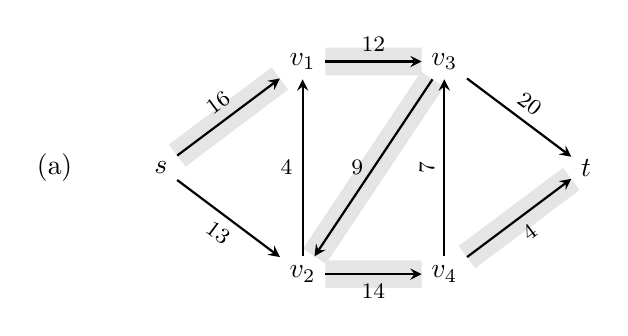
\begin{tikzpicture}[>=stealth, scale=0.9]
    % Nodes for graph (a)
    \node at (-1.5, 0) {(a)}; % Label for graph (a)
    \node (s) at (0, 0) {$s$};
    \node (v1) at (2, 1.5) {$v_1$};
    \node (v2) at (2, -1.5) {$v_2$};
    \node (v3) at (4, 1.5) {$v_3$};
    \node (v4) at (4, -1.5) {$v_4$};
    \node (t) at (6, 0) {$t$};

    % Highlighted augmenting path
    \draw[gray!20, line width=10pt, rounded corners] 
    (s) -- (v1) -- (v3) -- (v2) -- (v4) -- (t);
    
    % Edges with capacities
    \draw[->, thick] (s) -- (v1) node[midway, above, sloped, font=\footnotesize] {16};
    \draw[->, thick] (s) -- (v2) node[midway, below, sloped, font=\footnotesize] {13};
    \draw[->, thick] (v1) -- (v3) node[midway, above, sloped, font=\footnotesize] {12};
    \draw[->, thick] (v2) -- (v1) node[midway, left, font=\footnotesize] {4};
    \draw[->, thick] (v2) -- (v4) node[midway, below, sloped, font=\footnotesize] {14};
    \draw[->, thick] (v3) -- (v2) node[midway, left, font=\footnotesize] {9};
    \draw[->, thick] (v3) -- (t) node[midway, above, sloped, font=\footnotesize] {20};
    \draw[->, thick] (v4) -- (v3) node[midway, above, sloped, font=\footnotesize] {7};
    \draw[->, thick] (v4) -- (t) node[midway, below, sloped, font=\footnotesize] {4};
\end{tikzpicture}
\end{subfigure}
\hfill
\begin{subfigure}[t]{0.45\textwidth}
\centering
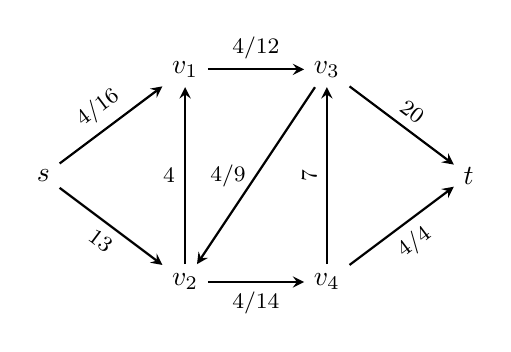
\begin{tikzpicture}[>=stealth, scale=0.9]
    % Nodes for the first graph on the right
    \node (s) at (0, 0) {$s$};
    \node (v1) at (2, 1.5) {$v_1$};
    \node (v2) at (2, -1.5) {$v_2$};
    \node (v3) at (4, 1.5) {$v_3$};
    \node (v4) at (4, -1.5) {$v_4$};
    \node (t) at (6, 0) {$t$};

    % Edges with flows/capacities
    \draw[->, thick] (s) -- (v1) node[midway, above, sloped, font=\footnotesize] {4/16};
    \draw[->, thick] (s) -- (v2) node[midway, below, sloped, font=\footnotesize] {13};
    \draw[->, thick] (v1) -- (v3) node[midway, above, sloped, font=\footnotesize] {4/12};
    \draw[->, thick] (v2) -- (v1) node[midway, left, font=\footnotesize] {4};
    \draw[->, thick] (v2) -- (v4) node[midway, below, sloped, font=\footnotesize] {4/14};
    \draw[->, thick] (v3) -- (v2) node[midway, left, font=\footnotesize] {4/9};
    \draw[->, thick] (v3) -- (t) node[midway, above, sloped, font=\footnotesize] {20};
    \draw[->, thick] (v4) -- (v3) node[midway, above, sloped, font=\footnotesize] {7};
    \draw[->, thick] (v4) -- (t) node[midway, below, sloped, font=\footnotesize] {4/4};
\end{tikzpicture}
\end{subfigure}

\vspace{0.25cm}

% Second row: (b) and the second graph
\begin{subfigure}[t]{0.45\textwidth}
\centering
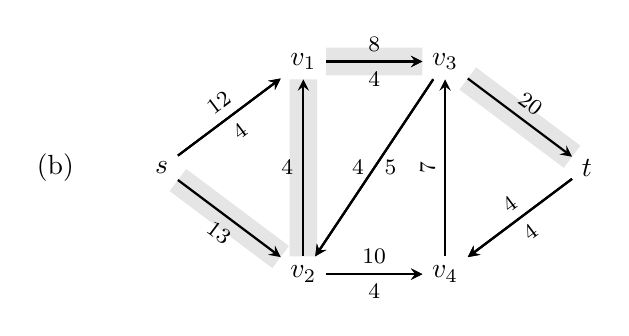
\begin{tikzpicture}[>=stealth, scale=0.9]
    % Nodes for graph (b)
    \node at (-1.5, 0) {(b)}; % Label for graph (b)
    \node (s) at (0, 0) {$s$};
    \node (v1) at (2, 1.5) {$v_1$};
    \node (v2) at (2, -1.5) {$v_2$};
    \node (v3) at (4, 1.5) {$v_3$};
    \node (v4) at (4, -1.5) {$v_4$};
    \node (t) at (6, 0) {$t$};

    % Highlighted augmenting path
    \draw[gray!20, line width=10pt, rounded corners] 
    (s) -- (v2) -- (v1) -- (v3) -- (t);

    % Forward Edges with capacities
    \draw[->, thick] (s) -- (v1) node[midway, above, sloped, font=\footnotesize] {12};
    \draw[->, thick] (s) -- (v2) node[midway, below, sloped, font=\footnotesize] {13};
    \draw[->, thick] (v1) -- (v3) node[midway, above, sloped, font=\footnotesize] {8};
    \draw[->, thick] (v2) -- (v1) node[midway, left, font=\footnotesize] {4};
    \draw[->, thick] (v2) -- (v4) node[midway, above, sloped, font=\footnotesize] {10};
    \draw[->, thick] (v3) -- (v2) node[midway, right, font=\footnotesize] {5};
    \draw[->, thick] (v3) -- (t) node[midway, above, sloped, font=\footnotesize] {20};
    \draw[->, thick] (v4) -- (v3) node[midway, above, sloped, font=\footnotesize] {7};
    \draw[<-, thick] (v4) -- (t) node[midway, below, sloped, font=\footnotesize] {4};

    % Reverse Edges with reverse capacities
    \draw[<-, thick] (v1) -- (s) node[midway, below, sloped, font=\footnotesize] {4};
    \draw[<-, thick] (v3) -- (v1) node[midway, below, sloped, font=\footnotesize] {4};
    \draw[<-, thick] (v2) -- (v3) node[midway, left, font=\footnotesize] {4};
    \draw[<-, thick] (v4) -- (v2) node[midway, below, sloped, font=\footnotesize] {4};
    \draw[->, thick] (t) -- (v4) node[midway, above, sloped, font=\footnotesize] {4};
\end{tikzpicture}
\end{subfigure}
\hfill
\begin{subfigure}[t]{0.45\textwidth}
\centering
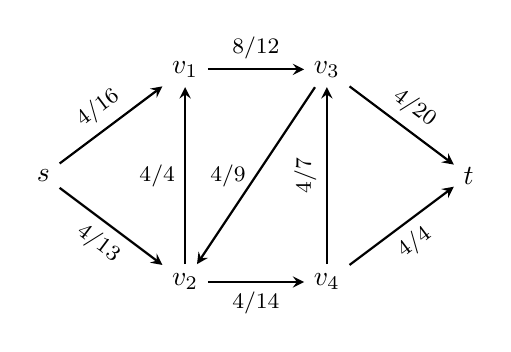
\begin{tikzpicture}[>=stealth, scale=0.9]
    % Nodes for the second graph on the right
    \node (s) at (0, 0) {$s$};
    \node (v1) at (2, 1.5) {$v_1$};
    \node (v2) at (2, -1.5) {$v_2$};
    \node (v3) at (4, 1.5) {$v_3$};
    \node (v4) at (4, -1.5) {$v_4$};
    \node (t) at (6, 0) {$t$};

    % Edges with flows/capacities
    \draw[->, thick] (s) -- (v1) node[midway, above, sloped, font=\footnotesize] {4/16};
    \draw[->, thick] (s) -- (v2) node[midway, below, sloped, font=\footnotesize] {4/13};
    \draw[->, thick] (v1) -- (v3) node[midway, above, sloped, font=\footnotesize] {8/12};
    \draw[->, thick] (v2) -- (v1) node[midway, left, font=\footnotesize] {4/4};
    \draw[->, thick] (v2) -- (v4) node[midway, below, sloped, font=\footnotesize] {4/14};
    \draw[->, thick] (v3) -- (v2) node[midway, left, font=\footnotesize] {4/9};
    \draw[->, thick] (v3) -- (t) node[midway, above, sloped, font=\footnotesize] {4/20};
    \draw[->, thick] (v4) -- (v3) node[midway, above, sloped, font=\footnotesize] {4/7};
    \draw[->, thick] (v4) -- (t) node[midway, below, sloped, font=\footnotesize] {4/4};
\end{tikzpicture}
\end{subfigure}

\vspace{0.25cm}

% Third row: (c) and the second graph
\begin{subfigure}[t]{0.45\textwidth}
\centering
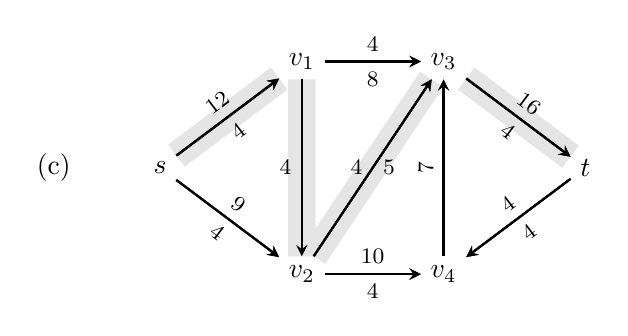
\begin{tikzpicture}[>=stealth, scale=0.9]
    % Nodes for graph (b)
    \node at (-1.5, 0) {(c)}; % Label for graph (c)
    \node (s) at (0, 0) {$s$};
    \node (v1) at (2, 1.5) {$v_1$};
    \node (v2) at (2, -1.5) {$v_2$};
    \node (v3) at (4, 1.5) {$v_3$};
    \node (v4) at (4, -1.5) {$v_4$};
    \node (t) at (6, 0) {$t$};

    % Highlighted augmenting path
    \draw[gray!20, line width=10pt, rounded corners] 
    (s) -- (v1) -- (v2) -- (v3) -- (t);

    % Forward Edges with capacities
    \draw[->, thick] (s) -- (v1) node[midway, above, sloped, font=\footnotesize] {12};
    \draw[->, thick] (s) -- (v2) node[midway, above, sloped, font=\footnotesize] {9};
    \draw[->, thick] (v1) -- (v3) node[midway, above, sloped, font=\footnotesize] {4};
    \draw[->, thick] (v1) -- (v2) node[midway, left, font=\footnotesize] {4};
    \draw[->, thick] (v2) -- (v4) node[midway, above, sloped, font=\footnotesize] {10};
    \draw[->, thick] (v2) -- (v3) node[midway, right, font=\footnotesize] {5};
    \draw[->, thick] (v3) -- (t) node[midway, above, sloped, font=\footnotesize] {16};
    \draw[->, thick] (v4) -- (v3) node[midway, above, sloped, font=\footnotesize] {7};
    \draw[->, thick] (t) -- (v4) node[midway, below, sloped, font=\footnotesize] {4};

     % Reverse Edges with reverse capacities
    \draw[<-, thick] (v1) -- (s) node[midway, below, sloped, font=\footnotesize] {4};
    \draw[<-, thick] (v2) -- (s) node[midway, below, sloped, font=\footnotesize] {4};
    \draw[<-, thick] (v3) -- (v1) node[midway, below, sloped, font=\footnotesize] {8};
    \draw[->, thick] (v2) -- (v3) node[midway, left, font=\footnotesize] {4};
    \draw[<-, thick] (v4) -- (v2) node[midway, below, sloped, font=\footnotesize] {4};
    \draw[->, thick] (t) -- (v4) node[midway, above, sloped, font=\footnotesize] {4};
    \draw[<-, thick] (t) -- (v3) node[midway, below, sloped, font=\footnotesize] {4};
\end{tikzpicture}
\end{subfigure}
\hfill
\begin{subfigure}[t]{0.45\textwidth}
\centering
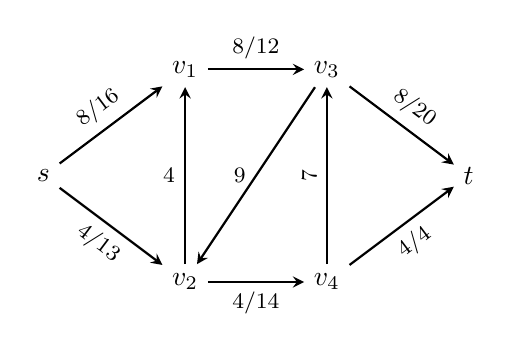
\begin{tikzpicture}[>=stealth, scale=0.9]
    % Nodes for the second graph on the right
    \node (s) at (0, 0) {$s$};
    \node (v1) at (2, 1.5) {$v_1$};
    \node (v2) at (2, -1.5) {$v_2$};
    \node (v3) at (4, 1.5) {$v_3$};
    \node (v4) at (4, -1.5) {$v_4$};
    \node (t) at (6, 0) {$t$};

    % Edges with flows/capacities
    \draw[->, thick] (s) -- (v1) node[midway, above, sloped, font=\footnotesize] {8/16};
    \draw[->, thick] (s) -- (v2) node[midway, below, sloped, font=\footnotesize] {4/13};
    \draw[->, thick] (v1) -- (v3) node[midway, above, sloped, font=\footnotesize] {8/12};
    \draw[->, thick] (v2) -- (v1) node[midway, left, font=\footnotesize] {4};
    \draw[->, thick] (v2) -- (v4) node[midway, below, sloped, font=\footnotesize] {4/14};
    \draw[->, thick] (v3) -- (v2) node[midway, left, font=\footnotesize] {9};
    \draw[->, thick] (v3) -- (t) node[midway, above, sloped, font=\footnotesize] {8/20};
    \draw[->, thick] (v4) -- (v3) node[midway, above, sloped, font=\footnotesize] {7};
    \draw[->, thick] (v4) -- (t) node[midway, below, sloped, font=\footnotesize] {4/4};
\end{tikzpicture}
\end{subfigure}

\caption{The execution of the basic Ford-Fulkerson algorithm. (a)–(e) Successive iterations of
the while loop. The left side of each part shows the residual network Gf from line 3 with a shaded
augmenting path p. The right side of each part shows the new flow f that results from augmenting f
by fp. The residual network in (a) is the input network G. The residual capacity $c_f$ is above/ on the left of each forward edge and is below/on the right of its reverse edge.}
\label{ff_graph(1)}
\end{figure}

\noindent The algorithm operates as follows:
\begin{enumerate}
    \item \textbf{Initialization:} Set $f(u, v) = 0$ for all edges $(u, v) \in E$.
    \item \textbf{Residual Network and Augmenting Paths:} 
    \begin{itemize}
        \item The algorithm operates on a residual network $G_f$, which represents how much additional flow can be pushed along each edge.
        \item For each edge $(u,v)$, the residual capacity $c_f(u,v)$ is calculated based on the edge’s capacity minus the current flow. 
        \item If a path from $s$ to $t$ exists in the residual network $G_f$ (with positive residual capacity on each edge), this path is called an augmenting path.
    \end{itemize}
    \item \textbf{Flow Augmentation:} 
    \begin{itemize}
        \item For each augmenting path $p$, determine the bottleneck capacity $c_f(p)$, which is the minimum residual capacity along that path.
        \item Increase the flow $f$ along the path $p$ by the residual capacity. Update the flow and residual capacities for each edge: If the edge is in the original direction, add the residual capacity to the flow. If the edge is in the reverse direction, subtract the residual capacity from the flow.
    \end{itemize}
    \item \textbf{Termination:} Repeat the process until there are no more augmenting paths in the residual network. When no augmenting paths are left, the flow $f$ represents the maximum flow from $s$ to $t$.
\end{enumerate}
The termination of the algorithm is validated by theorem \ref{max-flow theorem}, which states that a flow is maximized if and only if there are no augmenting paths left in the residual network.

%Second graph
\begin{figure}[ht]
\centering

% First row: (d) and the first graph
\begin{subfigure}[t]{0.45\textwidth}
\centering
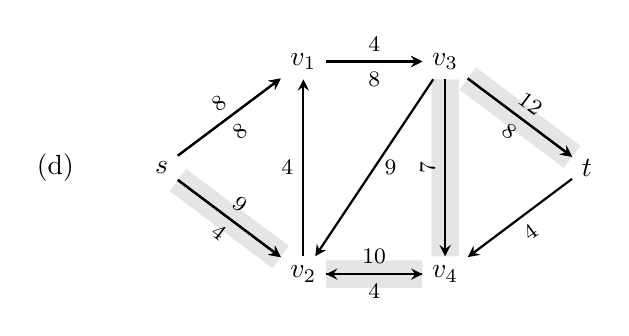
\begin{tikzpicture}[>=stealth, scale=0.9]
    % Nodes for graph (d)
    \node at (-1.5, 0) {(d)}; % Label for graph (a)
    \node (s) at (0, 0) {$s$};
    \node (v1) at (2, 1.5) {$v_1$};
    \node (v2) at (2, -1.5) {$v_2$};
    \node (v3) at (4, 1.5) {$v_3$};
    \node (v4) at (4, -1.5) {$v_4$};
    \node (t) at (6, 0) {$t$};

    % Highlighted augmenting path
    \draw[gray!20, line width=10pt, rounded corners] 
    (s) -- (v2) -- (v4) -- (v3) -- (t);
    
    % Edges with capacities
    \draw[->, thick] (s) -- (v1) node[midway, above, sloped, font=\footnotesize] {8};
    \draw[<-, thick] (v1) -- (s) node[midway, below, sloped, font=\footnotesize] {8};
    \draw[->, thick] (s) -- (v2) node[midway, above, sloped, font=\footnotesize] {9};
    \draw[->, thick] (s) -- (v2) node[midway, below, sloped, font=\footnotesize] {4};
    \draw[->, thick] (v1) -- (v3) node[midway, above, sloped, font=\footnotesize] {4};
    \draw[->, thick] (v1) -- (v3) node[midway, below, sloped, font=\footnotesize] {8};
    \draw[<-, thick] (v1) -- (v2) node[midway, left, font=\footnotesize] {4};
    \draw[->, thick] (v2) -- (v4) node[midway, above, sloped, font=\footnotesize] {10};
    \draw[<-, thick] (v2) -- (v4) node[midway, below, sloped, font=\footnotesize] {4};
    \draw[<-, thick] (v2) -- (v3) node[midway, right, font=\footnotesize] {9};
    \draw[->, thick] (v3) -- (t) node[midway, above, sloped, font=\footnotesize] {12};
    \draw[->, thick] (v3) -- (t) node[midway, below, sloped, font=\footnotesize] {8};
    \draw[<-, thick] (v4) -- (v3) node[midway, above, sloped, font=\footnotesize] {7};
    \draw[->, thick] (t) -- (v4) node[midway, below, sloped, font=\footnotesize] {4};
\end{tikzpicture}
\end{subfigure}
\hfill
\begin{subfigure}[t]{0.45\textwidth}
\centering
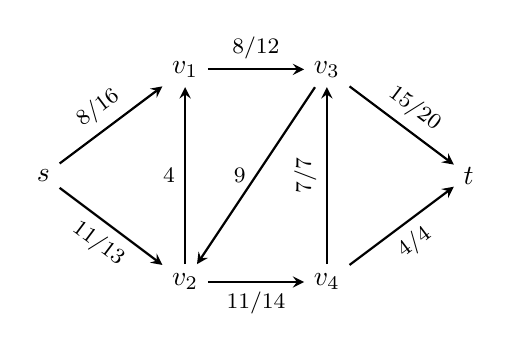
\begin{tikzpicture}[>=stealth, scale=0.9]
    % Nodes for the first graph on the right
    \node (s) at (0, 0) {$s$};
    \node (v1) at (2, 1.5) {$v_1$};
    \node (v2) at (2, -1.5) {$v_2$};
    \node (v3) at (4, 1.5) {$v_3$};
    \node (v4) at (4, -1.5) {$v_4$};
    \node (t) at (6, 0) {$t$};

    % Edges with flows/capacities
    \draw[->, thick] (s) -- (v1) node[midway, above, sloped, font=\footnotesize] {8/16};
    \draw[->, thick] (s) -- (v2) node[midway, below, sloped, font=\footnotesize] {11/13};
    \draw[->, thick] (v1) -- (v3) node[midway, above, sloped, font=\footnotesize] {8/12};
    \draw[->, thick] (v2) -- (v1) node[midway, left, font=\footnotesize] {4};
    \draw[->, thick] (v2) -- (v4) node[midway, below, sloped, font=\footnotesize] {11/14};
    \draw[->, thick] (v3) -- (v2) node[midway, left, font=\footnotesize] {9};
    \draw[->, thick] (v3) -- (t) node[midway, above, sloped, font=\footnotesize] {15/20};
    \draw[->, thick] (v4) -- (v3) node[midway, above, sloped, font=\footnotesize] {7/7};
    \draw[->, thick] (v4) -- (t) node[midway, below, sloped, font=\footnotesize] {4/4};
\end{tikzpicture}
\end{subfigure}

\vspace{0.25cm}

% Second row: (e) and the second graph
\begin{subfigure}[t]{0.45\textwidth}
\centering
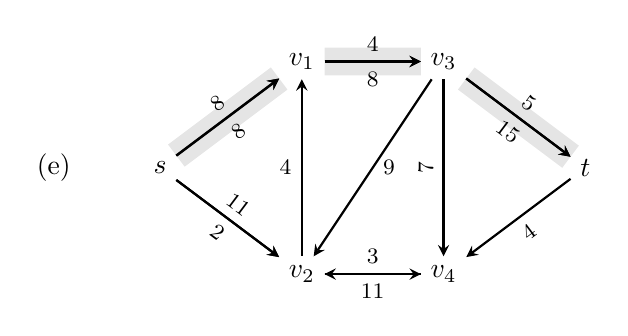
\begin{tikzpicture}[>=stealth, scale=0.9]
    % Nodes for graph (e)
    \node at (-1.5, 0) {(e)}; % Label for graph (e)
    \node (s) at (0, 0) {$s$};
    \node (v1) at (2, 1.5) {$v_1$};
    \node (v2) at (2, -1.5) {$v_2$};
    \node (v3) at (4, 1.5) {$v_3$};
    \node (v4) at (4, -1.5) {$v_4$};
    \node (t) at (6, 0) {$t$};

    % Highlighted augmenting path
    \draw[gray!20, line width=10pt, rounded corners] 
    (s) -- (v1) -- (v3) -- (t);

    % Edges with capacities
    \draw[->, thick] (s) -- (v1) node[midway, above, sloped, font=\footnotesize] {8};
    \draw[<-, thick] (v1) -- (s) node[midway, below, sloped, font=\footnotesize] {8};
    \draw[->, thick] (s) -- (v2) node[midway, above, sloped, font=\footnotesize] {11};
    \draw[->, thick] (s) -- (v2) node[midway, below, sloped, font=\footnotesize] {2};
    \draw[->, thick] (v1) -- (v3) node[midway, above, sloped, font=\footnotesize] {4};
    \draw[->, thick] (v1) -- (v3) node[midway, below, sloped, font=\footnotesize] {8};
    \draw[<-, thick] (v1) -- (v2) node[midway, left, font=\footnotesize] {4};
    \draw[->, thick] (v2) -- (v4) node[midway, above, sloped, font=\footnotesize] {3};
    \draw[<-, thick] (v2) -- (v4) node[midway, below, sloped, font=\footnotesize] {11};
    \draw[<-, thick] (v2) -- (v3) node[midway, right, font=\footnotesize] {9};
    \draw[->, thick] (v3) -- (t) node[midway, above, sloped, font=\footnotesize] {5};
    \draw[->, thick] (v3) -- (t) node[midway, below, sloped, font=\footnotesize] {15};
    \draw[<-, thick] (v4) -- (v3) node[midway, above, sloped, font=\footnotesize] {7};
    \draw[->, thick] (t) -- (v4) node[midway, below, sloped, font=\footnotesize] {4};
\end{tikzpicture}
\end{subfigure}
\hfill
\begin{subfigure}[t]{0.45\textwidth}
\centering
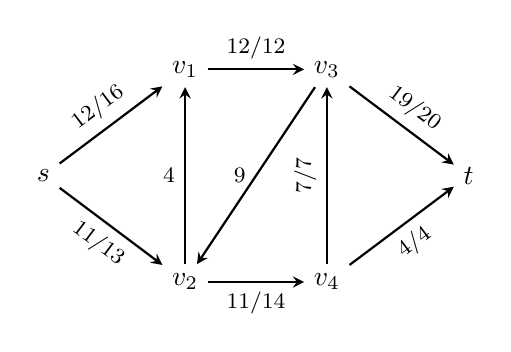
\begin{tikzpicture}[>=stealth, scale=0.9]
    % Nodes for the second graph on the right
    \node (s) at (0, 0) {$s$};
    \node (v1) at (2, 1.5) {$v_1$};
    \node (v2) at (2, -1.5) {$v_2$};
    \node (v3) at (4, 1.5) {$v_3$};
    \node (v4) at (4, -1.5) {$v_4$};
    \node (t) at (6, 0) {$t$};

    % Edges with flows/capacities
    \draw[->, thick] (s) -- (v1) node[midway, above, sloped, font=\footnotesize] {12/16};
    \draw[->, thick] (s) -- (v2) node[midway, below, sloped, font=\footnotesize] {11/13};
    \draw[->, thick] (v1) -- (v3) node[midway, above, sloped, font=\footnotesize] {12/12};
    \draw[->, thick] (v2) -- (v1) node[midway, left, font=\footnotesize] {4};
    \draw[->, thick] (v2) -- (v4) node[midway, below, sloped, font=\footnotesize] {11/14};
    \draw[->, thick] (v3) -- (v2) node[midway, left, font=\footnotesize] {9};
    \draw[->, thick] (v3) -- (t) node[midway, above, sloped, font=\footnotesize] {19/20};
    \draw[->, thick] (v4) -- (v3) node[midway, above, sloped, font=\footnotesize] {7/7};
    \draw[->, thick] (v4) -- (t) node[midway, below, sloped, font=\footnotesize] {4/4};
\end{tikzpicture}
\end{subfigure}

\vspace{0.25cm}

% Third row: (f) 
\begin{subfigure}[t]{0.45\textwidth}
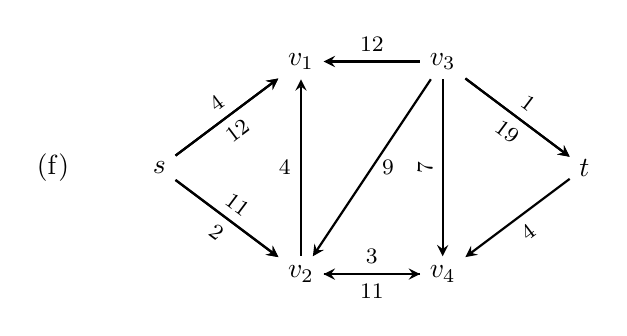
\begin{tikzpicture}[>=stealth, scale=0.9]
    % Nodes for graph (f)
    \node at (-1.5, 0) {(f)}; % Label for graph (f)
    \node (s) at (0, 0) {$s$};
    \node (v1) at (2, 1.5) {$v_1$};
    \node (v2) at (2, -1.5) {$v_2$};
    \node (v3) at (4, 1.5) {$v_3$};
    \node (v4) at (4, -1.5) {$v_4$};
    \node (t) at (6, 0) {$t$};

    % Forward Edges with capacities
    \draw[->, thick] (s) -- (v1) node[midway, above, sloped, font=\footnotesize] {4};
    \draw[<-, thick] (v1) -- (s) node[midway, below, sloped, font=\footnotesize] {12};
    \draw[->, thick] (s) -- (v2) node[midway, above, sloped, font=\footnotesize] {11};
    \draw[->, thick] (s) -- (v2) node[midway, below, sloped, font=\footnotesize] {2};
    \draw[<-, thick] (v1) -- (v3) node[midway, above, sloped, font=\footnotesize] {12};
    \draw[<-, thick] (v1) -- (v2) node[midway, left, font=\footnotesize] {4};
    \draw[->, thick] (v2) -- (v4) node[midway, above, sloped, font=\footnotesize] {3};
    \draw[<-, thick] (v2) -- (v4) node[midway, below, sloped, font=\footnotesize] {11};
    \draw[<-, thick] (v2) -- (v3) node[midway, right, font=\footnotesize] {9};
    \draw[->, thick] (v3) -- (t) node[midway, above, sloped, font=\footnotesize] {1};
    \draw[->, thick] (v3) -- (t) node[midway, below, sloped, font=\footnotesize] {19};
    \draw[<-, thick] (v4) -- (v3) node[midway, above, sloped, font=\footnotesize] {7};
    \draw[->, thick] (t) -- (v4) node[midway, below, sloped, font=\footnotesize] {4};
\end{tikzpicture}
\end{subfigure}
\caption{\textbf{(f)} The residual network at the last while loop test. It has no augmenting
paths and the flow $f$ shown in (e) is therefore a maximum flow. The value of the maximum flow
found is 23}
\label{ff_graph(2)}
\end{figure}

% Example 
\paragraph{Example:} Given a graph with the residual network (a) from Figure \ref{ff_graph(1)}. We can go through the Ford-Fulkerson algorithm to find the maximum flow showed in (e) from Figure \ref{ff_graph(2)}:\\
\textbf{Initialization}: Set $f(u, v) = 0$ for all edges $(u, v) \in E$. The initial flow in the network is zero, and the residual capacities are equal to the original capacities.\\
\textbf{Residual Network and Augmenting Paths:} The algorithm constructs a residual network $G_f$, where each edge $(u, v)$ has a residual capacity:$c_f(u, v) = c(u, v) - f(u, v)$. Paths in $G_f$ with positive residual capacities are called augmenting paths. The augmenting paths for the example are as follows:
\par Path 1: $p1: s \to v_1 \to v_3 \to v_2 \to v_4 \to t$, residual capacity:
\par \quad $ c_f(p1)$ = $min(c_f(s,v1), c_f(v1,v3), c_f(v3,v2), c_f(v2,v4), c_f(v4,t))$ = $min(16, 12, 9, 14, 4)=4$.
\par Path 2: $p2: s \to v_2 \to v_1 \to v_3 \to t$, \quad $c_f(p2)=4$.
\par Path 3: $p3: s \to v_1 \to v_2 \to v_3 \to t$, \quad $c_f(p3)=4$.
\par Path 4: $p4: s \to v_2 \to v_4 \to v_3 \to t$, \quad $c_f(p4)=7$.
\par Path 5: $p5: s \to v_1 \to v_3 \to t$, \quad $c_f(p5)=4$.
\\
\textbf{Flow Augmentation:} For each augmenting path $p$, the flow $f$ is increased by the residual capacity $c_f(p)$. After each augmentation, the residual network $G_f$ is updated as follows:

\par Path 1: $s \to v_1 \to v_3 \to v_2 \to v_4 \to t$. The residual capacity $c_f(p) = 4$. 
\par \quad Flow Update: $f(s, v_1) = 4$, $f(v_1, v_3) = 4$, $f(v_3, v_2) = 4$, $f(v_2, v_4) = 4$, $f(v_4, t) = 4$.
\par \quad Residual update:
\par\quad Forward edges: $c_f(s, v_1) = 16 - 4 = 12, \quad c_f(v_1, v_3) = 12 - 4 = 8, \quad c_f(v_3, v_2) = 9 - 4 = 5, \quad c_f(v_2, v_4) = 14 - 4 = 10, \quad c_f(v_4, t) = 4 - 4 = 0$.
\par \quad Reverse edges: $ c_f(v_1, s) = 4, \quad c_f(v_3, v_1) = 4, \quad c_f(v_2, v_3) = 4, \quad c_f(v_4, v_2) = 4, \quad c_f(t, v_4) = 4$.

\par Path 2: $s \to v_2 \to v_1 \to v_3 \to t$. The residual capacity $c_f(p) = 4$. 
\par \quad Flow Update: $f(s, v_2) = 4, \quad f(v_2, v_1) = 4, \quad f(v_1, v_3) = 8, \quad f(v_3, t) = 4.$.
\par \quad Residual update: 
\par \quad Forward edges: $c_f(s, v_2) = 13 - 4 = 9, \quad c_f(v_2, v_1) = 4 - 4 = 0, \quad c_f(v_1, v_3) = 8 - 4 = 4, \quad c_f(v_3, t) = 20 - 4 = 16$.
\par \quad Reverse edges: $c_f(v_2, s) = 4, \quad c_f(v_1, v_2) = 4, \quad c_f(v_3, v_1) = 8, \quad c_f(t, v_3) = 4$.

\par Path 3: $s \to v_1 \to v_2 \to v_3 \to t$. The residual capacity $c_f(p) = 4$. 
\par \quad Flow Update: $f(s, v_1) = 8$, $f(v_1, v_2) = 4$, $f(v_2, v_3) = 4$, $f(v_3, t) = 8$.
\par \quad Forward edges: $c_f(s, v_1) = 12 - 4 = 8, \quad c_f(v_1, v_2) = 4 - 4 = 0, \quad c_f(v_2, v_3) = 10 - 4 = 6, \quad c_f(v_3, t) = 16 - 4 = 12$.
\par \quad Reverse edges: $c_f(v_1, s) = 4, \quad c_f(v_2, v_1) = 4, \quad c_f(v_3, v_2) = 4, \quad c_f(t, v_3) = 8$.

\par Path 4: $s \to v_2 \to v_4 \to v_3 \to t$. The residual capacity $c_f(p) = 7$. 
\par \quad Flow Update: $f(s, v_2) = 11$, $f(v_2, v_4) = 11$, $f(v_4, v_3) = 7$, $f(v_3, t) = 15$.
\par \quad Forward edges: $c_f(s, v_2) = 9 - 7 = 2, \quad c_f(v_2, v_4) = 10 - 7 = 3, \quad c_f(v_4, v_3) = 7 - 7 = 0, \quad c_f(v_3, t) = 12 - 7 = 5$.
\par \quad Reverse edges: $c_f(v_2, s) = 7, \quad c_f(v_4, v_2) = 7, \quad c_f(v_3, v_4) = 7, \quad c_f(t, v_3) = 7$.

\par Path 5: $s \to v_1 \to v_3 \to t$. The residual capacity $c_f(p) = 4$. Update:
$f(s, v_1) = 12$, $f(v_1, v_3) = 12$, $f(v_3, t) = 19$.
\par \quad Forward edges: $c_f(s, v_1) = 8 - 4 = 4, \quad c_f(v_1, v_3) = 4 - 4 = 0, \quad c_f(v_3, t) = 5 - 4 = 1$.
\par \quad Reverse edges: $c_f(v_1, s) = 4, \quad c_f(v_3, v_1) = 4, \quad c_f(t, v_3) = 4$.

\textbf{Termination:} When no more augmenting paths exist in the residual network $G_f$, the algorithm terminates. The final flow $f$ is: $f(s, v_1) = 12, \quad f(s, v_2) = 11, \quad f(v_1, v_3) = 12, \quad f(v_2, v_4) = 11, \quad f(v_4, v_3) = 7, \quad f(v_3, t) = 19$. The maximum flow is the total flow out of $s$, which is: $|f| = f(s, v_1) + f(s, v_2) = 12 + 11 = 23$.


\paragraph{Performance and Time Complexity}
The Ford-Fulkerson method has a time complexity of $O(E \cdot F)$ where $E$ is the number of edges and 
$F$ is the maximum possible flow in the network. For networks with integer capacities, the algorithm guarantees termination in finite steps, though in cases with irrational capacities, it may not converge. 




\subsection{Hungarian Algorithm}
\label{subsec:hungarian}
% Author @ Ryan Feneley, IN-PROGRESS, Reviewer @ Ethan K, Due Date 11/19
The Hungarian Algorithm, also known as the Kuhn-Munkres algorithm, is a combinatorial optimization method used for finding maximum matchings in bipartite graphs. This algorithm is particularly notable for its ability to efficiently solve the assignment problem, where the objective is to assign \( n \) workers to \( n \) jobs in such a way that minimizes the total cost or maximizes the total profit. The algorithm operates by constructing a perfect matching in a weighted bipartite graph through a series of augmenting paths.

\paragraph{History}
The Hungarian Algorithm was first introduced by Harold Kuhn in 1955 \cite{kuhn1955hungarian}, based on earlier work by Hungarian mathematicians Dénes Kőnig and Jenő Egerváry. The algorithm was later refined by James Munkres in 1957 \cite{munkres1957algorithms}, resulting in a more efficient implementation that became widely adopted. This refinement not only improved the algorithm's practical usability but also solidified its theoretical foundations. The algorithm’s name honors the Hungarian mathematicians whose ideas inspired Kuhn’s work, underscoring its deep roots in combinatorial optimization.

\paragraph{Algorithm Overview}
The Hungarian algorithm operates in polynomial time and is based on the principle of finding an optimal assignment for weighted bipartite graphs. It aims to maximize or minimize the total weight of the matching, depending on the problem context. The process can be summarized in the following key steps:
\begin{enumerate}
    \item Initialization: Construct an initial feasible solution by subtracting the smallest value in each row and column of the cost matrix. This step simplifies the problem by ensuring that zero-cost entries exist in the matrix.
    \item Labeling and Reduction: Identify unmatched rows and columns, then adjust the labels to maintain feasibility. This involves modifying the cost matrix to preserve zeros while ensuring that the solution remains optimal.
    \item Finding Augmenting Paths: Construct alternating paths to update the current matching. Augmenting paths are sequences of alternating matched and unmatched edges, which are used to improve the matching incrementally.
    \item Iterative Refinement: Repeat the labeling and augmentation steps until a perfect matching is achieved. The final matching will minimize (or maximize) the total cost, depending on the objective.
\end{enumerate}

The algorithm maintains a feasible solution throughout its execution, ensuring that each step incrementally improves the matching. By systematically adjusting the labels and augmenting the matching, it guarantees an optimal solution.

\paragraph{Performance and Time Complexity}
The Hungarian algorithm runs in \(O(n^3)\) time, where \(n\) is the number of vertices in the bipartite graph. While this time complexity is polynomial, it can become computationally expensive for very large graphs. For instance, in real-time or large-scale applications with millions of vertices, alternative methods like auction algorithms or push-relabel methods may offer better scalability. Nevertheless, for moderate-sized problems, the Hungarian algorithm remains a reliable and practical choice.

Recent advancements have sought to reduce the computational overhead of the Hungarian algorithm. Variants that exploit sparsity in the cost matrix or incorporate parallel computing have been proposed, further expanding its applicability to larger datasets.

\paragraph{Applications}
The Hungarian algorithm has widespread applications across numerous domains:
\begin{itemize}
    \item Assignment Problems: Its most well-known application is in job assignment problems, where the algorithm determines the most efficient allocation of workers to tasks based on individual costs or efficiencies.
    \item Resource Allocation: The algorithm is used in logistics to optimize the distribution of goods or resources, such as matching trucks to delivery routes or allocating materials to production lines.
    \item Transportation Problems: In transportation networks, the Hungarian algorithm can optimize route planning by minimizing travel costs or time.
    \item Network Design: It finds use in computer networks to assign resources like bandwidth or servers to clients efficiently.
    \item Education and Scheduling: The algorithm has been applied to allocate classrooms, teachers, and resources in educational settings.
    \item Biological Research: In bioinformatics, it is used for problems such as protein-protein interaction matching or DNA sequencing alignment.
\end{itemize}

\paragraph{Advantages and Limitations}
The Hungarian algorithm is prized for its ability to guarantee an optimal solution for assignment problems in bipartite graphs. Unlike heuristic or approximation methods, it provides exact results, making it ideal for applications where precision is critical. Additionally, its systematic approach to augmenting paths and maintaining feasibility ensures robustness.

However, the \(O(n^3)\) time complexity makes it less suitable for extremely large graphs or real-time applications. In such cases, approximate or heuristic methods like the auction algorithm may be more practical. Additionally, the algorithm is tailored for bipartite graphs, meaning it cannot directly address non-bipartite or hypergraph matching problems without significant modifications.

\paragraph{Further Impact}
The Hungarian algorithm's development marked a significant milestone in the study of maximum matchings and laid the groundwork for subsequent advancements in matching theory. The algorithm's ability to handle weighted bipartite graphs inspired the creation of related methods for non-bipartite graphs, such as Edmonds' Blossom algorithm \cite{edmonds1965paths}.

\paragraph{Summary}
The Hungarian algorithm remains a foundational method in combinatorial optimization. Its capacity to deliver exact solutions for bipartite matching problems has ensured its continued relevance in diverse fields, including operations research, logistics, computer science, and biology. Despite its computational limitations for large-scale graphs, it remains an essential tool for solving assignment problems, showcasing the enduring value of foundational algorithms in modern applications.


\subsection{Dinic's Algorithm}
\label{subsec:dinics}
%\subsubsection*{Dinic's Algorithm (1970)}

Following the Ford-Fulkerson method and the Edmonds-Karp algorithm, Dinic's Algorithm provides a more efficient framework for solving the maximum flow problem in networks. Dinic's Algorithm was originally introduced by Israeli computer scientist Yefim (Chaim) Dinitz in 1970. While primarily designed for general graphs, Dinic's Algorithm can effectively solve the maximum matching problem in bipartite graphs by modeling the matching as a flow problem. \cite{dinitz1970algorithm}.

\paragraph{Algorithm Overview}

To apply Dinic's Algorithm to the bipartite matching problem, the bipartite graph $G=(U,V,E)$ is transformed into a flow network $G'=(V',E')$ following the procedure outlined in Section~3.6.2, where:
\begin{itemize}
    \item $V'$ is the new set of vertices containing original vertices in $U$ and $V$, plus a source $s$ and a sink $t$.
    \item $E'$ is the new set of edges in which, for every edge $(u,v) \in E$, $u \in U$ and $v \in V$ are connected with capacity 1.
\end{itemize}

The maximum flow in this transformed network corresponds to the maximum matching in the bipartite graph, where each flow unit represents an edge in the matching \cite{cormen2009introduction}.

\textbf{Dinic’s Algorithm} can be divided into three main phases:
\begin{enumerate}
    \item The algorithm begins by constructing a level graph $L$. A level graph is derived from the residual graph $G(f)$, which represents the current state of flow in the network. $L$ ensures only edges forming the shortest augmenting paths (refer to Section~2.1.11 for definition) are considered in subsequent steps. A level graph is constructed by performing Breadth-First Search (BFS) from the source to assign levels to vertices based on the distance from $s$.
    \begin{figure}[ht]
        \centering
        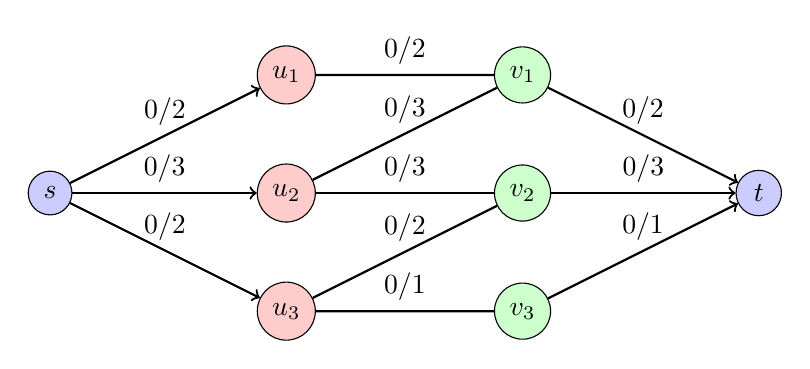
\begin{tikzpicture}[scale=1.5]
            % Draw nodes for source and sink
            \node[circle, draw, fill=blue!20] (s) at (-2, 0) {\(s\)};

            \node[circle, draw, fill=blue!20] (t) at (4, 0) {\(t\)};

        
            % Draw nodes for set U
            \node[circle, draw, fill=red!20] (u1) at (0, 1) {\(u_1\)};
            \node[circle, draw, fill=red!20] (u2) at (0, 0) {\(u_2\)};
            \node[circle, draw, fill=red!20] (u3) at (0, -1) {\(u_3\)};

        
            % Draw nodes for set V
            \node[circle, draw, fill=green!20] (v1) at (2, 1) {\(v_1\)};
            \node[circle, draw, fill=green!20] (v2) at (2, 0) {\(v_2\)};
            \node[circle, draw, fill=green!20] (v3) at (2, -1) {\(v_3\)};

        
            % Draw edges from source to set U
            \draw[thick, ->] (s) -- node[midway, above] {0/2} (u1);
            \draw[thick, ->] (s) -- node[midway, above] {0/3} (u2);
            \draw[thick, ->] (s) -- node[midway, above] {0/2} (u3);
            
        
            % Draw edges between U and V
            \draw[thick] (u1) -- node[midway, above] {0/2} (v1); % Edge between u1 and v1
            \draw[thick] (u2) -- node[midway, above] {0/3} (v1); % Edge between u2 and v1
            \draw[thick] (u2) -- node[midway, above] {0/3} (v2); % Edge between u2 and v2
            \draw[thick] (u3) -- node[midway, above] {0/2} (v2); % Edge between u3 and v2
            \draw[thick] (u3) -- node[midway, above] {0/1} (v3); % Edge between u3 and v3
        
            % Draw edges from set V to sink
            \draw[thick, ->] (v1) -- node[midway, above] {0/2} (t);
            \draw[thick, ->] (v2) -- node[midway, above] {0/3} (t);
            \draw[thick, ->] (v3) -- node[midway, above] {0/1} (t);
        
        \end{tikzpicture}
        \label{fig:level_graph}
        \caption{Initial graph \( G \) before BFS. All edges are shown with no level assignments.}
        \end{figure}
        

    \item Once the level graph \(L\) is constructed, the algorithm computes a \textit{blocking flow} in \(L\). A blocking flow is a flow such that no augmenting path from \(s\) to \(t\) exists within \(L\). This is achieved by identifying augmenting paths using Depth-First Search (DFS) and augmenting the flow along each path by the minimum residual capacity of the edges in the path. If an edge along a path is fully saturated (i.e., its residual capacity becomes zero), the path becomes invalid for further augmentation. By saturating at least one edge on every \(s \to t\) path, the algorithm ensures no further augmenting paths can exist in \(L\). After augmenting the flow, the residual capacities in the original graph \(G(f)\) are updated to reflect the changes. This process guarantees that the blocking flow fully utilizes the level graph for the current iteration before the next level graph is constructed.

    \begin{figure}[h]
        \centering
        \begin{tikzpicture}[scale=1.5]
            % Draw nodes for source and sink
            \node[circle, draw, fill=blue!20] (s) at (-2, 0) {\(s\)};
            \node[above=0.1cm of s] (L0) {\textbf{L0}};
            \node[circle, draw, fill=blue!20] (t) at (4, 0) {\(t\)};
            \node[above=0.1cm of t] (L3) {\textbf{L3}};
        
            % Draw nodes for set U
            \node[circle, draw, fill=red!20] (u1) at (0, 1) {\(u_1\)};
            \node[circle, draw, fill=red!20] (u2) at (0, 0) {\(u_2\)};
            \node[circle, draw, fill=red!20] (u3) at (0, -1) {\(u_3\)};

            \node[above=0.1cm of u1] (L1) {\textbf{L1}};
            \node[above=0.1cm of u2] (L1) {\textbf{L1}};
            \node[above=0.1cm of u3] (L1) {\textbf{L1}};
        
            % Draw nodes for set V
            \node[circle, draw, fill=green!20] (v1) at (2, 1) {\(v_1\)};
            \node[circle, draw, fill=green!20] (v2) at (2, 0) {\(v_2\)};
            \node[circle, draw, fill=green!20] (v3) at (2, -1) {\(v_3\)};
            \node[above=0.1cm of v1] (L2) {\textbf{L2}};
            \node[above=0.1cm of v2] (L2) {\textbf{L2}};
            \node[above=0.1cm of v3] (L2) {\textbf{L2}};
        
          % Draw edges from source to set U
          \draw[thick, ->] (s) -- node[midway, above] {0/2} (u1);
          \draw[thick, ->] (s) -- node[midway, above] {3/3} (u2);
          \draw[thick, ->] (s) -- node[midway, above] {2/2} (u3);
          
      
          % Draw edges between U and V
          \draw[thick] (u1) -- node[midway, above] {0/2} (v1); % Edge between u1 and v1
          \draw[thick] (u2) -- node[midway, above] {2/3} (v1); % Edge between u2 and v1
          \draw[thick] (u2) -- node[midway, above] {1/3} (v2); % Edge between u2 and v2
          \draw[thick] (u3) -- node[midway, above] {1/2} (v2); % Edge between u3 and v2
          \draw[thick] (u3) -- node[midway, above] {1/1} (v3); % Edge between u3 and v3
      
        % Draw edges from set V to sink
        \draw[thick, ->] (v1) -- node[midway, above] {2/2} (t);
        \draw[thick, ->] (v2) -- node[midway, above] {2/3} (t);
        \draw[thick, ->] (v3) -- node[midway, above] {1/1} (t);
        
        % Highlight shortest augmenting paths in BFS
        \draw[ultra thick, blue, ->] (s) -- (u2); % Shortest path to u2
        \draw[ultra thick, blue] (u2) -- (v1); % Shortest path from u2 to v1
        \draw[ultra thick, blue, ->] (v1) -- (t); % Shortest path to sink

        \draw[ultra thick, blue, ->] (s) -- (u3); % Shortest path to u2
        \draw[ultra thick, blue] (u3) -- (v3); % Shortest path from u2 to v1
        \draw[ultra thick, blue, ->] (v3) -- (t); % Shortest path to sink

        \draw[ultra thick, blue, ->] (s) -- (u2); % Shortest path to u2
        \draw[ultra thick, blue] (u2) -- (v2); % Shortest path from u2 to v1
        \draw[ultra thick, blue, ->] (v2) -- (t); % Shortest path to sink
        
        \draw[ultra thick, blue, ->] (s) -- (u3); % Shortest path to u2
        \draw[ultra thick, blue] (u3) -- (v2); % Shortest path from u2 to v1
        \draw[ultra thick, blue, ->] (v2) -- (t); % Shortest path to sink
        
        \end{tikzpicture}
        
        \label{fig:level_graph}
        \caption{Construction of the level graph \( L \) in Dinic's Algorithm, illustrating the level graph after performing BFS.}
        \end{figure}

\paragraph{}Figures above illustrate the process of constructing a level graph \( L \) from the initial graph \( G \) in Dinic's Algorithm. Figure 3.1 shows the initial graph \( G \), which represents the network before performing any operations. In this state, all edges and vertices are present, but no levels are assigned to the nodes. Figure 3.2 represents the level graph \( L \) after applying a Breadth-First Search (BFS) on the residual graph \( G(f) \). BFS begins from the source node \( s \) and assigns levels to vertices based on their shortest distance from \( s \). These levels, denoted as \( L0, L1, L2, \) and \( L3 \), correspond to increasing distances from the source. In the example, BFS finds a shortest augmenting path \( s \to u_2 \to v_1 \to t \), which is highlighted in blue. For the path \( s \to u_2 \to v_1 \to t \), maximum amount of flow that can be pushed along this path is $\min\{ c_f(s, u_2), c_f(u_2, v_1), c_f(v_1, t) \} = 2$. After that, it is added to the flow along each edge in the augmenting path, and we update the residual capacities. Notice how we are sending four flows together. This is where it is optimized compared to Edmond Karp where we send one flow at a time. 
\begin{itemize}
    \item 2 units of flow on path \( s \to u_2 \to v_1 \to t \)
    \item 1 unit of flow on path \( s \to u_3 \to v_3 \to t \)
    \item 1 unit of flow on path \( s \to u_3 \to v_2 \to t \)
    \item 1 unit of flow on path \( s \to u_2 \to v_2 \to t \)
    \item Total flow is:5
\end{itemize}

    
    \paragraph{} Now, since we achieve the first blocking flow iteration, we repeat the process by rebuilding the level graph. This time it should look different because the remaining capacities of multiple edges have changed.

    \begin{figure}[h]
        \centering
        \begin{tikzpicture}[scale=1.5]
            % Draw nodes for source and sink
            \node[circle, draw, fill=blue!20] (s) at (-2, 0) {\(s\)};
            \node[above=0.1cm of s] (L0) {\textbf{L0}};
            \node[circle, draw, fill=blue!20] (t) at (4, 0) {\(t\)};
            \node[above=0.1cm of t] (L3) {\textbf{L5}};
        
            % Draw nodes for set U
            \node[circle, draw, fill=red!20] (u1) at (0, 1) {\(u_1\)};
            \node[circle, draw, fill=red!20] (u2) at (0, 0) {\(u_2\)};
            \node[circle, draw, fill=red!20] (u3) at (0, -1) {\(u_3\)};

            \node[above=0.1cm of u1] (L1) {\textbf{L1}};
            \node[above=0.1cm of u2] (L3) {\textbf{L3}};
        
            % Draw nodes for set V
            \node[circle, draw, fill=green!20] (v1) at (2, 1) {\(v_1\)};
            \node[circle, draw, fill=green!20] (v2) at (2, 0) {\(v_2\)};
            \node[circle, draw, fill=green!20] (v3) at (2, -1) {\(v_3\)};
            \node[above=0.1cm of v1] (L2) {\textbf{L2}};
            \node[above=0.1cm of v2] (L2) {\textbf{L4}};
        
          % Draw edges from source to set U
          \draw[thick, ->] (s) -- node[midway, above] {1/2} (u1);
          \draw[thick, ->] (s) -- node[midway, above] {3/3} (u2);
          \draw[thick, ->] (s) -- node[midway, above] {2/2} (u3);
          
      
          % Draw edges between U and V
          \draw[thick] (u1) -- node[midway, above] {1/2} (v1); % Edge between u1 and v1
          \draw[thick] (u2) -- node[midway, above] {2/3} (v1); % Edge between u2 and v1
          \draw[thick] (u2) -- node[midway, above] {1/3} (v2); % Edge between u2 and v2
          \draw[thick] (u3) -- node[midway, above] {1/2} (v2); % Edge between u3 and v2
          \draw[thick] (u3) -- node[midway, above] {1/1} (v3); % Edge between u3 and v3
      
        % Draw edges from set V to sink
        \draw[thick, ->] (v1) -- node[midway, above] {2/2} (t);
        \draw[thick, ->] (v2) -- node[midway, above] {3/3} (t);
        \draw[thick, ->] (v3) -- node[midway, above] {1/1} (t);
        
        % Highlight shortest augmenting paths in BFS
        \draw[ultra thick, blue, ->] (s) -- (u1); % Shortest path to u2
        \draw[ultra thick, blue] (u1) -- (v1); % Shortest path from u2 to v1
        \draw[ultra thick, blue, ->] (v1) -- (u2); % Shortest path to sink
        \draw[ultra thick, blue, ->] (u2) -- (v2); % Shortest path to sink
        \draw[ultra thick, blue, ->] (v2) -- (t); % Shortest path to sink
        \end{tikzpicture}
        
        \label{fig:level_graph}
        \caption{Construction of the level graph \( L \) in Dinic's Algorithm, illustrating the level graph after performing BFS.}
        \end{figure}
    
    \paragraph{} After this phase:
    \begin{itemize}
        \item 1 unit of flow on path \( s \to u_1 \to v_1 \to u2 \to v2 \to t \)
        \item Total flow is: 5 + 1 = 6
    \end{itemize}

    \paragraph{} Here, a block flow is achieved, and there are no more flows can be pushed through the network. Program terminates.

                    
    \item The algorithm iterates between constructing a level graph and computing a blocking flow until no augmenting paths can be found, at which point the maximum flow (and thus the maximum matching) has been achieved.
\end{enumerate}

\paragraph{Pseudocode}
In the context of bipartite maximum matching, the input is a bipartite graph $G = (U, V, E)$, where $U$ and $V$ are two disjoint sets of vertices, and $E$ is the set of edges connecting them. As stated above, the problem is converted into a network flow: $G =((V,E),c,f,s,t)$. Dinic's Algorithm proceeds as follows:

\begin{algorithm}
    \caption{Dinic's Algorithm for Maximum Bipartite Matching}
    
    \textbf{Input:} A network \( G = ((V, E), c, s, t) \). \\
    \textbf{Output:} An \( s \)–\( t \) flow \( f \) of maximum value.
    
    \begin{algorithmic}[1]
    \STATE Initialize \( f(e) \gets 0 \) for each \( e \in E \).
    \WHILE{true}
        \STATE Construct the level graph \( G_L \) from the residual graph \( G(f) \) using BFS.
        \IF{\( \text{dist}(t) = \infty \)}
            \STATE \textbf{break} (No more augmenting paths exist).
        \ENDIF
        \WHILE{A blocking flow \( f' \) can be found in \( G_L \)}
            \STATE Augment the flow \( f \) by \( f' \).
            \STATE Update the residual capacities in \( G(f) \).
        \ENDWHILE
    \ENDWHILE
    \RETURN \( f \)
    \end{algorithmic}
    \end{algorithm}    

\paragraph{Explanation}

Going line by line:
\begin{itemize}
    \item \textbf{Line 1:} Initializes all flows $f(e)$ to zero for each edge $e \in E$.
    \item \textbf{Line 2-5:} A breadth-first search (BFS) is performed on the residual graph $G(f)$ to compute the shortest path distances $\text{dist}(v)$ from the source $s$ to every vertex $v$. Using these distances, the level graph $G(L)$ is built. This graph only includes edges $(u,v) \in E(f)$ that satisfy $\text{dist}(v)=\text{dist}(u)+1$. If $\text{dist}(t)=\infty$, no $s$-$t$ path exists, and the algorithm terminates, confirming that the current flow is the maximum flow.
    \item \textbf{Line 6:} A blocking flow $f'$ is computed within $G(L)$. This is a flow where every $s$-$t$ path in $G(L)$ has at least one saturated edge (i.e., flow equals capacity).
    \item \textbf{Line 7-8:} By definition, $f'$ ensures no further flow can be sent along any $s$-$t$ path in $G(L)$, completing the current iteration of the algorithm.
    \item \textbf{Line 9:} Return the maximum flow.
\end{itemize}

\paragraph{Performance and Time Complexity}

The level graph $G(L)$ is built using a breadth-first search (BFS) on the residual graph $G(f)$. BFS runs in $O(V + E)$ time, where $V$ is the number of vertices and $E$ is the number of edges. To find a blocking flow, the most common method is to use a depth-first search (DFS) approach. Each edge in $G(L)$ is traversed at most once during a single computation of $f'$, making the blocking flow computation run in $O(E)$. Augmenting the flow also takes $O(E)$ time.

In bipartite maximum matching problems, all edges have unit capacity. The residual graph's depth (or the number of levels in $G(L)$) is limited by the number of edges in the longest augmenting path. This depth is proportional to $O(\sqrt{V})$, as the level graph represents alternating layers of vertices in the bipartite structure. Hence, at most $O(\sqrt{V})$ level graphs are needed for the entire algorithm. This explains the $O(\sqrt{V} \cdot E)$ performance for bipartite graphs, where the algorithm iteratively builds and uses $O(\sqrt{V})$ level graphs, each requiring $O(E)$ work.

\paragraph{Applications and Limitations}

Dinic’s Algorithm has applications in diverse fields such as network optimization, scheduling, and resource allocation. It is particularly effective in bipartite matching problems, with uses in image segmentation, community detection, and compiler optimizations. However, it is less efficient for dense graphs due to $O(V^3)$ complexity when $E = O(V^2)$, reflecting the worst-case complexity in fully connected networks. $O(\sqrt{V} \cdot E)$ applies to sparse bipartite graphs, while the $O(V^3)$ upper bound applies in dense graph scenarios.



\subsection{Edmonds-Karp}
\label{subsec:edmonds_karp}
% Author @ Huyen Tran, DONE

%\subsection{Edmonds-Karp Algorithm}
\label{ek algo}

The \textbf{Edmonds-Karp algorithm}, developed by Jack Edmonds and Richard Karp in 1972, is an implementation of the Ford-Fulkerson method for computing the maximum flow in a flow network by using \textbf{breadth-first search (BFS)} to find the shortest augmenting paths in terms of edge count. \cite{edmonds_karp_1972}

\subsubsection*{Algorithm Overview}
The Edmonds-Karp algorithm operates in polynomial time and is based on the principle of finding the maximum flow in a flow network by augmenting flows along shortest paths. The process begins by initializing the flow at zero and constructing an initial feasible solution in the residual network. It then iteratively increases the flow by finding augmenting paths—shortest paths from the source to the sink in terms of edge count in the residual network—until no more augmenting paths exist, indicating an optimal solution.

\noindent In each iteration, the algorithm identifies the shortest augmenting path using BFS and adjusts the flow along this path by its minimum residual capacity. This approach ensures that each augmentation moves the flow closer to the maximum flow while maintaining a feasible flow throughout its execution. By using BFS to select augmenting paths, the Edmonds-Karp algorithm achieves a more efficient and practical implementation of the Ford-Fulkerson method, widely adopted for solving maximum flow problems in various fields.

\noindent The algorithm would take a graph instance \( G = (d, n, m, E) \), with parameters:
        \begin{itemize}
            \item \( d \): The degree of vertices in the matching,
            \item \( n \): The number of vertices on each side of the bipartite graph,
            \item \( m \): The number of edges, and
            \item \( E \): The set of edges connecting left and right vertex sets.
        \end{itemize}
        
\paragraph{Example:}
Below is an example bipartite graph with sets \( U = \{ u_1, u_2, u_3 \} \) and \( V = \{ v_1, v_2, v_3 \} \). The maximum matching is highlighted in red.

\begin{figure}[h!]
\centering
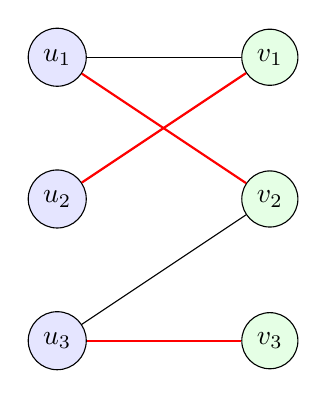
\begin{tikzpicture}[scale=0.9, every node/.style={circle, draw, minimum size=0.4cm}]
    % Nodes in U
    \node[fill=blue!10] (u1) at (0,2) {$u_1$};
    \node[fill=blue!10] (u2) at (0,0) {$u_2$};
    \node[fill=blue!10] (u3) at (0,-2) {$u_3$};
    
    % Nodes in V
    \node[fill=green!10] (v1) at (3,2) {$v_1$};
    \node[fill=green!10] (v2) at (3,0) {$v_2$};
    \node[fill=green!10] (v3) at (3,-2) {$v_3$};
    
    % Edges (Non-matching in black)
    \draw (u1) -- (v1);
    \draw (u1) -- (v2);
    \draw (u2) -- (v1);
    \draw (u3) -- (v2);
    \draw (u3) -- (v3);
    
    % Matching edges in red
    \draw[thick, red] (u2) -- (v1);
    \draw[thick, red] (u1) -- (v2);
    \draw[thick, red] (u3) -- (v3);
\end{tikzpicture}
\caption{A solved instance of the Maximum Matching Problem with $d = 2$, $|V| = 3$, $|E| = 5$. The black lines show the edges of $E$. The three edges highlighted in red are a maximum matching $M = \{ (u_1, v_2), (u_2, v_1), (u_3, v_3) \} $ of $G$.}
\label{fig:ex_bipartite_graph}
\end{figure}

\noindent Given the graph \( G = \{2, 3, 5, ((1,1), (1,2), (2,1), (3,2), (3,3)) \} \) as Figure \ref{fig:ex_bipartite_graph}, we can trace the Edmonds-Karp algorithm as follows:

\textbf{Initialization:} The residual graph is constructed with a source node \( s \) and sink node \( t \). Capacities are assigned such that:
\begin{itemize}
    \item \( c(s, u_i) = 1 \) for all \( u_i \in U \),
    \item \( c(v_j, t) = 1 \) for all \( v_j \in V \),
    \item \( c(u_i, v_j) = 1 \) for all \( (u_i, v_j) \in E \).
\end{itemize}
\par Initially, all flows \( f(u, v) \) are set to zero, and the residual capacities are equal to the original capacities.\\

\textbf{First Augmenting Path:} Using BFS, the algorithm identifies the first augmenting path:
$s \to u_1 \to v_1 \to t$.
\par The residual capacity of this path is: $c_f(p_1) = \min(c_f(s, u_1), c_f(u_1, v_1), c_f(v_1, t)) = \min(1, 1, 1) = 1.$
\par Flow Update:$f(s, u_1) = 1, \quad f(u_1, v_1) = 1, \quad f(v_1, t) = 1$.
\par Forward edges' residual capacities: $c_f(s, u_1) = 0, \quad c_f(u_1, v_1) = 0, \quad c_f(v_1, t) = 0.$
\par Reverse edges' capacities: $c_f(u_1, s) = 1, \quad c_f(v_1, u_1) = 1, \quad c_f(t, v_1) = 1.$\\

\textbf{Second Augmenting Path:} BFS finds another augmenting path: $s \to u_2 \to v_2 \to t.$
\par The residual capacity of this path is: $c_f(p_2) = \min(c_f(s, u_2), c_f(u_2, v_2), c_f(v_2, t)) = \min(1, 1, 1) = 1.$
\par Flow Update: $f(s, u_2) = 1, \quad f(u_2, v_2) = 1, \quad f(v_2, t) = 1.$
\par Forward edges' residual capacities: $c_f(s, u_2) = 0, \quad c_f(u_2, v_2) = 0, \quad c_f(v_2, t) = 0.$
\par Reverse edges' capacities: $c_f(u_2, s) = 1, \quad c_f(v_2, u_2) = 1, \quad c_f(t, v_2) = 1.$\\

\textbf{Third Augmenting Path:} BFS identifies another path: $s \to u_3 \to v_3 \to t.$
\par The residual capacity of this path is: $c_f(p_3) = \min(c_f(s, u_3), c_f(u_3, v_3), c_f(v_3, t)) = \min(1, 1, 1) = 1.$
\par Flow Update: $f(s, u_3) = 1, \quad f(u_3, v_3) = 1, \quad f(v_3, t) = 1.$
\par Forward edges' residual capacities: $c_f(s, u_3) = 0, \quad c_f(u_3, v_3) = 0, \quad c_f(v_3, t) = 0.$
\par Reverse edges' capacities: $c_f(u_3, s) = 1, \quad c_f(v_3, u_3) = 1, \quad c_f(t, v_3) = 1.$\\

\textbf{Termination:} BFS is unable to find any additional augmenting paths, as no path from $s$ to $t$ with positive residual capacity exists. The algorithm terminates.

\textbf{Extracting the Matching:} The matching is extracted by identifying edges $(u_i, v_j)$ in the residual graph where reverse edges \( (v_j, u_i) \) have positive capacity. The resulting maximum matching is:
\[
M = \{ (u_1, v_2), (u_2, v_1), (u_3, v_3) \}.
\]
\par This matching corresponds to the edges highlighted in red in the original graph.


\subsubsection*{Performance and Time Complexity}

The Edmonds-Karp algorithm has a time complexity of \(\mathcal{O}(VE^2)\), which is polynomial in the number of vertices \( V \) and edges \( E \) of the graph. The analysis of this complexity relies on two key theoretical results, a lemma and a theorem, which bound the number of augmenting paths and explain how the structure of the residual network changes over time.

\begin{lemma}
If the Edmonds-Karp algorithm is run on a flow network \( G = (V, E) \) with source \( s \) and sink \( t \), then for all vertices \( v \in V \setminus \{s, t\} \), the shortest-path distance \( \delta_f(s, v) \) in the residual network \( G_f \) increases monotonically with each flow augmentation.
\end{lemma}
This lemma states that in the Edmonds-Karp algorithm, the shortest-path distance \( \delta_f(s, v) \) from the source \( s \) to any vertex \( v \) in the residual network \( G_f \) either increases or remains constant with each flow augmentation. This property ensures that distances in the residual network do not decrease, helping to limit the number of augmenting paths that can be selected over the course of the algorithm.

\begin{theorem}
    If the Edmonds-Karp algorithm is run on a flow network \( G = (V, E) \) with source \( s \) and sink \( t \), then the total number of flow augmentations performed by the algorithm is \( O(VE) \).
\end{theorem}
This theorem states that the total number of augmenting paths required by the Edmonds-Karp algorithm to reach the maximum flow is \(\mathcal{O}(VE)\). Each edge in the residual network can become critical (limiting the residual capacity of a path) at most \(\mathcal{O}(V)\) times. This bound prevents the algorithm from cycling inefficiently through paths, as each critical edge reappearance increases the shortest-path distance of involved vertices, further limiting augmenting path frequency.

Together, these results guarantee that the Edmonds-Karp algorithm performs only a limited, polynomial number of augmentations. Each BFS search to find an augmenting path takes \( \mathcal{O}(E) \) time, leading to an overall complexity of \( \mathcal{O}(VE^2) \).\\

\noindent Further details and implementation of this algorithm is discussed in Section \ref{ekImplement}


\subsection{Hopcroft-Karp}
\label{subsec:hopcroft_karp}
% Author @ Ryan Feneley, IN-PROGRESS, Reviewer @ Ethan K, Due Date 11/19

The Hopcroft-Karp Algorithm, introduced by John Hopcroft and Richard Karp in 1973, is a foundational algorithm for finding the maximum matching in bipartite graphs. By incorporating an innovative multi-phase approach, the algorithm significantly improved upon earlier methods, such as the Ford-Fulkerson algorithm \cite{ford1956flows}, which only found a single augmenting path per iteration. The Hopcroft-Karp algorithm’s ability to process multiple augmenting paths in parallel not only improved efficiency but also established it as one of the most widely used algorithms for bipartite matching. 

\paragraph{Historical Context}
Before the Hopcroft-Karp Algorithm, most methods for finding maximum matchings in bipartite graphs relied on augmenting path-based strategies, such as those in the Ford-Fulkerson algorithm. However, these approaches suffered from inefficiencies, especially in large, sparse graphs. Hopcroft and Karp addressed this challenge by introducing a BFS-DFS hybrid strategy, which optimized the discovery and utilization of augmenting paths. Their work not only advanced the study of bipartite matching but also inspired subsequent research into graph algorithms and network optimization.

\paragraph{Algorithm Overview}
The Hopcroft-Karp Algorithm operates by alternating between two main phases, leveraging the concepts of graphs and augmenting paths:

\begin{itemize}
    \item \textbf{Phase 1: Breadth-First Search (BFS)}:
    The algorithm begins by constructing a level graph using BFS. This involves grouping vertices by their distance from unmatched vertices in the current matching. The BFS ensures that the algorithm focuses on the shortest augmenting paths, which are critical for improving the matching efficiently. Each layer of the graph corresponds to vertices that can be reached via alternating paths of increasing lengths.

    \item \textbf{Phase 2: Depth-First Search (DFS)}:
    After the level graph is constructed, the algorithm employs DFS to discover all augmenting paths in the graph. Unlike earlier approaches that find and process a single path at a time, the Hopcroft-Karp algorithm finds and processes multiple disjoint augmenting paths simultaneously. Once these paths are identified, the edges along them are flipped, incrementally increasing the size of the matching.
\end{itemize}

This two-phase process—constructing the level graph followed by finding disjoint augmenting paths—repeats iteratively until no more augmenting paths can be found. At this point, the current matching is guaranteed to be maximum due to the absence of any further augmenting paths, as described by Berge's theorem \cite{berge1957two}.

\paragraph{Performance and Time Complexity}
The Hopcroft-Karp algorithm achieves a time complexity of \(O(\sqrt{V}E)\), where \(V\) is the number of vertices and \(E\) is the number of edges. This represents a significant improvement over the \(O(VE)\) complexity of the Ford-Fulkerson algorithm \cite{ford1956flows}. The reduction in complexity is primarily due to the algorithm's ability to process multiple augmenting paths in a single iteration, minimizing the number of expensive BFS and DFS traversals.

This improvement is particularly impactful in large, sparse graphs, where the number of edges \(E\) is much smaller than the square of the number of vertices \(V\). The algorithm’s efficiency makes it a practical choice for solving large-scale bipartite matching problems in real-world applications.

\paragraph{Applications}
The Hopcroft-Karp algorithm has been applied extensively in various domains due to its reliability and efficiency:
\begin{itemize}
    \item Job Assignment Problems:
    In scenarios where workers must be assigned to jobs based on cost or efficiency, the Hopcroft-Karp algorithm provides an optimal solution by maximizing the number of matched pairs.
    
    \item Network Flows:
    The algorithm is used in network flow problems, particularly in constructing maximum flows in bipartite networks.
    
    \item Data Matching:
    It can aid in linking records and data deduplication, where the goal is to find the best match between two datasets.
    
    \item Pairing:
    The algorithm is employed in scheduling tasks in bipartite structures, such as pairing machines to tasks or classrooms to teachers.
    
    \item Graph Analytics:
    In social network analysis, the algorithm identifies meaningful relationships in bipartite structures, such as connections between users and items.
\end{itemize}

\paragraph{Strengths and Limitations}
The Hopcroft-Karp algorithm is particularly well-suited for problems involving bipartite graphs due to its efficient handling of augmenting paths. Its ability to process multiple paths in parallel significantly reduces computational overhead in sparse graphs, making it a preferred choice for large-scale applications.

However, the algorithm is limited to bipartite graphs and cannot directly address matching problems in general (non-bipartite) graphs. For such cases, algorithms like Edmonds' Blossom Algorithm \cite{edmonds1965paths} are necessary. Furthermore, while the \(O(\sqrt{V}E)\) complexity is efficient, there are more modern algorithms tailored for specific problem instances, such as very dense or weighted graphs, that may outperform Hopcroft-Karp in practice.

\paragraph{Theoretical Impact}
The Hopcroft-Karp algorithm not only advanced the study of graph matching but also demonstrated the power of hybrid search strategies in graph algorithms. Its introduction of the BFS-DFS combination as a core methodology inspired subsequent work in graph theory, network flow algorithms, connectivity, and traversal.

\paragraph{Summary}
The Hopcroft-Karp algorithm is fundamental in the study of bipartite graph matching. Its efficient handling of augmenting paths, combined with its applicability to a wide range of practical problems, ensures its continued relevance in both theoretical research and real-world applications. Despite its limitations in addressing non-bipartite graphs, its efficiency and robustness make it one of the most significant advancements in graph algorithm design, and it remains to this day the standard for bupartite matchings.


\subsection{Bipartite Perfect Matching}
% @author Huyen Tran, Claudia Porto DONE
\label{matrix-perfect-matching}
Marcin Mucha and Piotr Sankowski introduced new methods for finding perfect matching for both general and bipartite graphs which are based on randomization. The running time of these methods is $O(n^\omega)$, where $\omega$ is the smallest number such that two n×n matrices can be multiplied together. The current best-known value of $\omega$ is less than 2.38. These methods are easy to implement in $O(n^3)$ time, with the only tricky part being the fast matrix multiplication. \cite{Mucha-Sankowski}.

\subsubsection*{Matchings, Adjacency Matrices, and Their Inverses}
The method uses the mathematical framework that connects graph theory and linear algebra, focusing on matchings in graphs and their representation through adjacency matrices. By examining skew symmetric adjacency matrices and their properties, we can gain insights into the existence and identification of perfect matchings. This exploration also includes the development of algorithms, both randomized and deterministic, to efficiently determine matchings in bipartite graphs.

\paragraph*{Skew Symmetric Adjacency Matrix:} A matrix \( A \) is skew symmetric if \( A^T = -A \), meaning the transpose of \( A \) is equal to the negative of \( A \). The transpose of a matrix refers to the operation of flipping the matrix over its diagonal, so the rows of the original matrix become the columns in the transposed matrix, and vice versa. 
\noindent For a given graph \( G = (V, E) \), a skew-symmetric adjacency matrix \( \tilde{A}(G) \) is constructed with entries defined as:
\[
\tilde{A}_{i,j}(G) =
\begin{cases} 
x_{i,j} & \text{if } (v_i, v_j) \in E \text{ and } i < j, \\
-x_{i,j} & \text{if } (v_i, v_j) \in E \text{ and } i > j, \\
0 & \text{otherwise}.
\end{cases}
\]
Here, $x_{i,j}$ are unique variables assigned to edges in $E$. According to Tutte's theorem, the symbolic determinant \( \det \tilde{A}(G) \) is non-zero if and only if $G$ has a perfect matching.

\noindent To determine a perfect matching, unique random values are substituted for the symbolic variables, resulting in a random adjacency matrix \( A(G) \). By the Schwartz-Zippel lemma, with high probability, \( \det A(G) \neq 0 \) indicates the presence of a perfect matching. This leads to a randomized algorithm for determining if a graph has a perfect matching by computing the determinant of $A(G)$. The same method applies to bipartite graphs, where the symbolic determinant of the bipartite adjacency matrix is non-zero if the graph has a perfect matching. This can be done in $O(n^\omega)$ time using fast matrix multiplication. 

\noindent For example, given a graph $G=(V,E)$ with \( U = \{ u_1, u_2, u_3 \} \) and \( V = \{ v_1, v_2, v_3 \} \) and \\
$E=\{(v1,u1), (v1,u3), (v2,u1), (v3,u2), (v3,u3)\}$ represented in Figure \ref{fig:pm graph} , we can generate a the skew-symmetric adjacency matrix and then assign random value for each edge as in Figure \ref{fig:matrices}
\begin{figure}[h!]
\centering
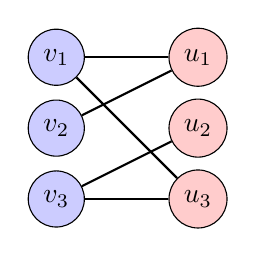
\begin{tikzpicture}[scale=0.9, every node/.style={circle, draw, minimum size=0.4cm}]
    % Define coordinates for the left (V) and right (U) sets
    \node[fill=blue!20] (v1) at (0, 2) {$v_1$};
    \node[fill=blue!20] (v2) at (0, 1) {$v_2$};
    \node[fill=blue!20] (v3) at (0, 0) {$v_3$};
    
    \node[fill=red!20] (u1) at (2, 2) {$u_1$};
    \node[fill=red!20] (u2) at (2, 1) {$u_2$};
    \node[fill=red!20] (u3) at (2, 0) {$u_3$};
    
    % Draw edges between the sets
    \draw[thick] (v1) -- (u1);
    \draw[thick] (v1) -- (u3);
    \draw[thick] (v2) -- (u1);
    \draw[thick] (v3) -- (u2);
    \draw[thick] (v3) -- (u3);
\end{tikzpicture}
\caption{Representation of graph $G=(V,E)$ with \( U = \{ u_1, u_2, u_3 \} \) and \( V = \{ v_1, v_2, v_3 \} \) and
$E=\{(v1,u1), (v1,u3), (v2,u1), (v3,u2), (v3,u3)\}$.}
\label{fig:pm graph}
\end{figure}

\begin{figure}[h]
    \centering
    % First matrix (a)
    \begin{subfigure}[b]{0.4\textwidth}
        \centering
        \[
        \tilde{A}(G) =
        \begin{bmatrix}
        0 & 0 & 0 & x_{1,1} & 0 & x_{1,3} \\
        0 & 0 & 0 & -x_{2,1} & 0 & 0 \\
        0 & 0 & 0 & 0 & -x_{3,2} & x_{3,3} \\
        -x{1,1} & -x_{2,1} & 0 & 0 & x_{4,5} & 0 \\
        0 & 0 & x_{3,2} & 0 & 0 & 0 \\
        -x_{1,3} & 0 & -x_{3,3} & 0 & 0 & 0
        \end{bmatrix}
        \]
        \caption{Symbolic skew-symmetric adjacency matrix (a).}
    \end{subfigure}
    \hfill
    % Second matrix (b)
    \begin{subfigure}[b]{0.4\textwidth}
        \centering
        \[
        \tilde{A}(G) =
        \begin{bmatrix}
        0 & 0 & 0 & 3 & 0 & 7 \\
        0 & 0 & 0 & -5 & 0 & 0 \\
        0 & 0 & 0 & 0 & -8 & 4 \\
        -3 & 5 & 0 & 0 & 0 & 0 \\
        0 & 0 & 8 & 0 & 0 & 0 \\
        -7 & 0 & -4 & 0 & 0 & 0
        \end{bmatrix}
        \]
        \caption{Randomized adjacency matrix with assigned weights (b).}
    \end{subfigure}
    \caption{Comparison of the symbolic skew-symmetric adjacency matrix (a) and the randomized adjacency matrix (b).}
    \label{fig:matrices}
\end{figure}

\paragraph*{Matrix Rank and Maximum Matching:}
Lovasz extended the approach by showing that the rank of \( A(G) \) equals twice the size of the maximum matching in \( G \) with high probability. This forms the basis for algorithms that compute the determinant or rank of \( A(G) \) using randomized substitutions and fast matrix operations. For example, \( O(n^\omega) \) time complexity is achieved for determinant computation, where \( \omega \) is the matrix multiplication exponent, currently \( \omega < 2.38 \).

\paragraph*{Allowed Edges:}
To construct a perfect matching, the algorithm identifies \textbf{allowed edges}, edges guaranteed to belong to some perfect matching. Using matrix inversion, Rabin and Vazirani showed that the inverse matrix \( A^{-1}(G) \) provides edge information: if \( (v_i, v_j) \in E \), then \( A^{-1}_{j,i} \neq 0 \) implies that \( (v_i, v_j) \) is an allowed edge.

\noindent The algorithm iteratively identifies an allowed edge, removes its endpoints from \( G \), and updates the adjacency matrix \( A(G') \) for the reduced graph \( G' \). By employing Gaussian elimination techniques and leveraging the Schur complement, the matrix updates are performed efficiently to avoid recomputation, maintaining an \( O(n^\omega) \) runtime.


\subsubsection{Constructing Matchings via Gaussian Elimination} 
The construction of matchings uses Gaussian elimination to systematically reduce the adjacency matrix of the graph while preserving information about perfect matchings. This process ensures computational efficiency and avoids recomputing matrices from scratch.

\paragraph*{Schur Complement and Matrix Update:}
Given a random adjacency matrix \( A(G) \) of a bipartite graph \( G = (U, V, E) \), let \( A^{-1}(G) \) be its inverse. If an edge \( (u_1, v_1) \in E \) satisfies \( A^{-1}_{1,1} \neq 0 \), then \( (u_1, v_1) \) is an \textbf{allowed edge} and can be chosen as part of the matching. However, recomputing \( A^{-1}(G) \) for the reduced graph \( G' = G - \{u_1, v_1\} \) from scratch would result in an \( O(n^{\omega+1}) \) algorithm. Instead, the Elimination Theorem states that the inverse of a submatrix can be updated using the Schur complement. The Schur complement is a derived matrix that provides a more efficient update mechanism.\\
Given a block matrix:
\[
A = \begin{bmatrix}
A_{11} & A_{12} \\
A_{21} & A_{22}
\end{bmatrix}
\]
where \(A_{11}\) and \(A_{22}\) are square matrices, the Schur complement of \(A_{22}\) in \(A\) is defined as:
\[
S = A_{11} - A_{12} A_{22}^{-1} A_{21}
\]
The Schur complement \(S\) is used to update the inverse of the submatrix \(A_{11}\) when \(A_{22}\) is inverted. This is particularly useful in the context of Gaussian elimination.\\
Therefore, when 
\[
A = 
\begin{bmatrix}
a_{1,1} & \mathbf{v}^T \\
\mathbf{u} & B
\end{bmatrix},
\quad
A^{-1} = 
\begin{bmatrix}
\hat{a}_{1,1} & \hat{\mathbf{v}}^T \\
\hat{\mathbf{u}} & \hat{B}
\end{bmatrix},
\]
\[
\text{where } \hat{a}_{1,1} \neq 0. \text{ Then } B^{-1} = \hat{B} - \frac{\hat{\mathbf{u}} \hat{\mathbf{v}}^T}{\hat{a}_{1,1}}.
\]

\noindent This result enables an efficient \( O(n^3) \) algorithm for finding perfect matchings using iterative updates without recomputation of the full matrix.

\paragraph*{Simple Algorithms for Perfect Matchings:}
Using Gaussian elimination, the following algorithms for perfect matching are defined:
\begin{enumerate}
    \item \textbf{Bipartite Graphs:} For bipartite graphs, the algorithm iteratively eliminates rows and columns corresponding to matched vertices while maintaining the inverse of the updated matrix. Allowed edges are identified by non-zero entries in \( A^{-1} \).
    \item \textbf{General Graphs:} For general graphs, additional elimination steps ensure symmetry in row and column updates. The process guarantees that allowed edges are correctly preserved.
\end{enumerate}

The algorithms for perfect matchings follow this general structure:
\begin{algorithm}
\caption{Simple algorithm for perfect matchings in bipartite graphs}
\textsc{Simple-Bipartite-Matching}($G$):
\begin{algorithmic}[1]
    \STATE $B = A^{-1}(G)$
    \STATE $M = \emptyset$
    \FOR{$c = 1$ to $n$}
        \STATE find a row $r$, not yet eliminated, and such that $B_{r,c} \neq 0$ and $A(G)_{c,r} \neq 0$ (i.e. $(u_c, v_r)$ is an allowed edge in $G - V(M)$)
        \STATE eliminate the $r$-th row and the $c$-th column of $B$
        \STATE add $(u_c, v_r)$ to $M$
    \ENDFOR
\end{algorithmic}
\end{algorithm}

Both algorithms achieve \( O(n^3) \) complexity due to efficient elimination and matrix inversion techniques.

\noindent \textbf{Example of Simple Bipartite Matching:} Given the graph $G=(E,V)$ in Figure \ref{fig:pm graph}, with the skew-symmetric adjacency matrix $A(G)$ in Figure \ref{fig:matrices}. Since the adjacency matrix \( A(G) \) can be represented as a block matrix:
\[
A(G) = 
\begin{bmatrix}
0 & A_{12} \\
A_{21} & 0
\end{bmatrix},
\]
where \( A_{12} \) corresponds to the edges from \( V \) to \( U \), and \( A_{21} = -A_{12}^T \) because $G$ is a bipartite graph. The matrix \( A_{12} \) is given by:
\[
A_{12} =
\begin{bmatrix}
3 & 0 & 7 \\
-5 & 0 & 0 \\
0 & -8 & 4
\end{bmatrix}.
\]
We can find the perfect matching in $G$ using the \textit{Simple-Bipartite-Matching} algorithm as follows:\\
\textbf{Initialization.} We compute the inverse of \( A = A_{12} \), denoted as \( B = A^{-1} \), which will be used to trace through the algorithm. For this example:
\[
\renewcommand{\arraystretch}{1.5}
B =
\begin{bmatrix}
0 & -\frac{1}{5} & 0 \\
\frac{1}{14} & \frac{3}{70} & -\frac{1}{8} \\
\frac{1}{7} & \frac{3}{35} & 0
\end{bmatrix}.
\]

\textbf{$c=1$: } Pick edge \( (v_2, u_1) \). Because \( B_{2,1} = \frac{1}{14} \neq 0 \) and \(A_{12} = -5 \neq 0 \) , which makes it valid. Therefore, add \( (v_2, u_1) \) to the matching and remove \( v_2 \) and \( u_1 \) from the graph, and update \( B \):
\[
\renewcommand{\arraystretch}{1.5}
B =
\begin{bmatrix}
0 & -\frac{1}{5} & 0 \\
0 & 0 & 0 \\
\frac{13}{98} & \frac{39}{490} & \frac{1}{56}
\end{bmatrix}.
\]

\textbf{$c=2$: } Pick edge \( (v_3, u_2) \). Because \( B_{3,2} = \frac{39}{490} \neq 0 \) and \(A_{12} = -8 \neq 0 \) , which makes it valid. Therefore, add \( (v_3, u_2) \) to the matching, remove \( v_3 \) and \( u_2 \) from the graph, and update \( B \):
\[
\renewcommand{\arraystretch}{1.5}
B =
\begin{bmatrix}
\frac{13}{195} & -\frac{117}{650} & \frac{1}{28} \\
0 & 0 & 0 \\
-\frac{13}{49} & -\frac{117}{163} & 0
\end{bmatrix}.
\]

\textbf{$c=3$: } Pick edge \( (v_1, u_3) \). Because \( B_{1,3} = \frac{1}{28} \neq 0 \) and \(A_{12} = 7 \neq 0 \) , which makes it valid. Therefore, add \( (v_1, u_3) \) to the matching and remove \( v_1 \) and \( u_3 \) from the graph, and update \( B \):
\[
\renewcommand{\arraystretch}{1.5}
B =
\begin{bmatrix}
0 & 0 & 0 \\
0 & 0 & 0 \\
-\frac{13}{49} & -\frac{117}{163} & 0
\end{bmatrix}.
\]

\textbf{Result:} The final perfect matching is: $M = \{(v_1, u_3), (v_2, u_1), (v_3, u_2)\}.$


\paragraph*{Matching Verification and Lazy Elimination:}
To verify matchings and find maximal allowed submatchings, a simplified version of Gaussian elimination, called \textbf{lazy elimination}, is employed. Instead of updating all matrix elements immediately, changes are accumulated in compact forms, such as \( \mathbf{u} \mathbf{v}^T / c \), and applied in batches during critical steps. This approach allows verification of inclusion-wise maximal matchings in \( O(n^\omega) \) time.

\begin{algorithm}
\caption{Gaussian elimination with no pivoting}
\textsc{Simple-Elimination}($X$):
\begin{algorithmic}[1]
    \FOR{$i = 1$ to $n$}
        \STATE lazily eliminate the $i$-th row and $i$-th column of $X$;
        \STATE let $j$ be the largest integer such that $2^j \mid i$;
        \STATE \textbf{UPDATE}($\{i + 1, \ldots, i + 2^j\}, \{i + 1, \ldots, n\}$);
        \STATE \textbf{UPDATE}($\{i + 2^j + 1, \ldots, n\}, \{i + 1, i + 2^j\}$);
    \ENDFOR
\end{algorithmic}
\end{algorithm}

\textbf{Example of Gaussian Elimination with No Pivoting}

Consider the following matrix $A(G)$:
\[
A(G) = 
\begin{bmatrix} 
1 & 0 & 1 \\
1 & 1 & 0 \\
0 & 1 & 1
\end{bmatrix}
\]

\begin{enumerate} 
\item \textbf{Eliminate the first row and column:} 
    \begin{itemize}
        \item The first element \( A_{1,1} = 1 \) is already non-zero
         \item Subtract the first row from the second row to eliminate the first column in the second row:
        \[
        \begin{bmatrix} 
        1 & 0 & 1 \\
        0 & 1 & -1 \\
        0 & 1 & 1
        \end{bmatrix}
        \]
        \item Subtract the first row from the third row to eliminate the first column in the third row:
        \[
        \begin{bmatrix} 
        1 & 0 & 1 \\
        0 & 1 & -1 \\
        0 & 1 & 1
        \end{bmatrix}
        \]
    \end{itemize}

\item \textbf{Eliminate the second row and column:}
    \begin{itemize}
        \item The second element \( A_{2,2} = 1 \) is non-zero.
        \item Subtract the second row from the third row to eliminate the second column in the third row:
        \[
        \begin{bmatrix} 
        1 & 0 & 1 \\
        0 & 1 & -1 \\
        0 & 0 & 2
        \end{bmatrix}
        \]
    \end{itemize} 

\item \textbf{Eliminate the third row and column:}
    \begin{itemize}
        \item The third element \( A_{3,3} = 2 \) is non-zero.
        \item No further elimination is needed as we have reached the last row.
    \end{itemize}
\end{enumerate}

The resulting upper triangular matrix is:
\[
U = 
\begin{bmatrix} 
1 & 0 & 1 \\
0 & 1 & -1 \\
0 & 0 & 2
\end{bmatrix}
\]

To find an inclusion-wise maximal allowed submatching, we can use the resulting upper triangular matrix \( U \). The non-zero entries in \( U \) indicate the allowed submatchings. In this case, the non-zero entries are:
\begin{itemize}
    \item \( U_{1,1} = 1 \)
    \item \( U_{2,2} = 1 \)
    \item \( U_{3,3} = 2 \)
\end{itemize}
These entries correspond to the inclusion-wise maximal allowed submatching.

\paragraph{Performance and Time Complexity}
The algorithm has a time complexity of $O(n^\omega)$, where $n$ is the number of vertices in the graph and $\omega$ is the matrix multiplication exponent (currently $\omega < 2.38$). The algorithm leverages randomized substitutions and efficient matrix operations, such as determinant computation and matrix inversion, to identify allowed edges and construct a perfect matching. While the algorithm is probabilistic (Monte Carlo), the error probability can be made arbitrarily small by choosing a sufficiently large finite field for the random substitutions. In practice, the algorithm is highly efficient for dense graphs, as its complexity depends on matrix multiplication rather than the number of edges.

\noindent Further details and implementation of this algorithm is discussed in Section \ref{pmReduction}


\section{D-Partite Graph Algorithms}
\label{sec:dpartite_algorithms}

\subsection{Brute-Force}
\label{subsec:brute_force}
% Author: Ryan Feneley, IN-PROGRESS, Reviewer: Ethan K, Due Date: 11/19

Brute-force algorithms for solving the maximum matching problem in \(d\)-partite graphs provide a conceptually simple yet computationally intensive approach. These algorithms systematically explore all possible matchings to identify the one with the maximum cardinality or weight. While they guarantee an exact solution, their applicability is severely limited by their exponential time complexity, making them practical only for small or highly constrained graphs \cite{garey1979computers}.

\paragraph{Algorithm Mechanism}
The brute-force approach involves the following steps:
\begin{enumerate}
    \item Enumeration of Matchings:
    All potential matchings are generated by iterating through subsets of edges that satisfy the matching condition (i.e., no two edges share a vertex).
    \item Validation:
    Each subset is validated to ensure it forms a feasible matching within the \(d\)-partite graph structure.
    \item Evaluation:
    For weighted graphs, the total weight of each matching is computed. For unweighted graphs, the cardinality is calculated.
    \item Optimization:
    The algorithm selects the matching with the maximum weight or cardinality from the evaluated candidates.
\end{enumerate}

This exhaustive search ensures that no possible matching is overlooked, making it the most straightforward but computationally demanding solution.

\paragraph{Performance and Complexity}
The primary limitation of brute-force algorithms is their exponential time complexity, \(O(d!)\) for a \(d\)-partite graph, due to the need to evaluate all possible combinations of edges. As the number of partitions and vertices increases, the computational burden grows exponentially, rendering the approach infeasible for large graphs.

Despite this, brute-force methods are occasionally used as a baseline for comparison in theoretical studies or as a fallback solution for small-scale problems where computational resources are not a constraint.

\paragraph{Applications}
Brute-force algorithms, while inefficient, have specific niches in which they remain relevant:
\begin{itemize}
    \item Proof-of-Concept Studies:
    They serve as a benchmark for evaluating the performance and accuracy of heuristic or approximation algorithms.
    \item Specialized Small-Scale Problems:
    For small \(d\)-partite graphs with tightly constrained parameters, brute-force methods can provide guaranteed solutions.
    \item Algorithm Development:
    They are often used in the design and testing phases of more sophisticated algorithms to validate correctness and completeness.
\end{itemize}

\paragraph{Strengths and Limitations}
The brute-force approach is straightforward to implement and guarantees optimal solutions. However, its exponential time complexity severely restricts its practical utility, particularly for large \(d\)-partite graphs or real-world applications where computational efficiency is crucial. The method is also limited in its ability to handle dynamic or evolving graphs, as any change necessitates a complete recomputation of the matching.

\paragraph{Conclusion}
While brute-force algorithms are rarely used in practice for solving the maximum matching problem in \(d\)-partite graphs, they remain a valuable theoretical tool. Their simplicity and guaranteed optimality make them a useful reference point in algorithm design and complexity analysis. However, for practical applications, more efficient algorithms, such as heuristic or approximation methods, are almost always preferred.


\subsection{Ant Colony Optimization (ACO)}
\label{subsec:aco}
Ant Colony Optimization (ACO) is a \textit{metaheuristic} algorithm inspired by the behavior of real ants, particularly their foraging behavior, which involves depositing pheromones to guide other ants toward food sources. A metaheuristic refers to a higher-level procedure designed to find, generate, or select a heuristic that can provide good solutions to complex optimization problems, often by exploring a large solution space in a way that is not guaranteed to be optimal, but likely to be good enough in a reasonable time frame. This nature-inspired algorithm, introduced by Marco Dorigo in the early 1990s, has been successfully applied to a variety of NP-hard and NP-complete problems, such as the Traveling Salesman Problem (TSP), vehicle routing, and network optimization \cite{Dorigo2004}. One particularly challenging NP-hard problem is the Maximum Matching Problem which is essential in fields like network design, job assignments, and resource allocation.

This book explores how ACO can be adapted to solve the Maximum Matching Problem. The sections following describe how ACO works,its adaptation for solving the Maximum Matching Problem, and its application in other NP-hard problems.

\subsubsection*{Background on Ant Colony Optimization}

Ant Colony Optimization (ACO) mimics the way real ants use pheromones to communicate and find optimal paths between their nest and a food source. As illustrated in figure ~\ref{fig:ant_pheromone_path}, the diagram demonstrates this behavior in a simplified form. The nest (represented by the yellow circle) is located at the origin, while the food source (red circle) is positioned at a distance. Ants travel along different paths, each marked by different colors which represent different pheromone trails. In the diagram, the \textbf{high pheromone trail} (blue line) represents the optimal path, where ants have reinforced the trail most frequently. The \textbf{medium pheromone trail} (black line) and \textbf{low pheromone trail} (red line) represent paths that have seen less traffic and, therefore, lower pheromone concentrations.
 

\begin{figure}[t]
\centering
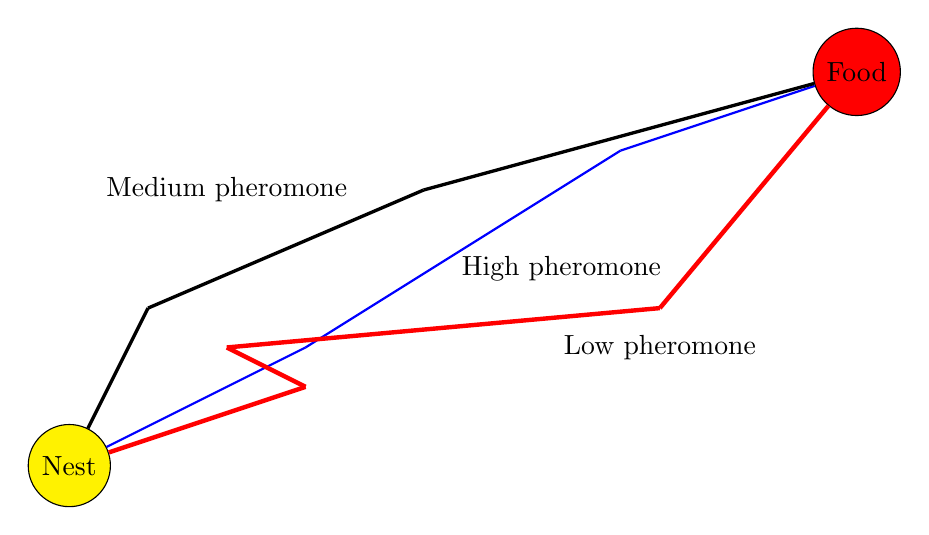
\begin{tikzpicture}
    % Define nodes for nest and food source
    \node[draw, circle, fill=yellow] (nest) at (0, 0) {Nest};
    \node[draw, circle, fill=red] (food) at (10, 5) {Food};

    % Ant paths with varying pheromone strengths (represented by line thickness)
    \draw[thick, color=blue] (nest) -- (3, 1.5);
    \draw[thick, color=blue] (3, 1.5) -- (7, 4);
    \draw[thick, color=blue] (7, 4) -- (food);

    \draw[very thick] (nest) -- (1, 2);
    \draw[very thick] (1, 2) -- (4.5, 3.5);
    \draw[very thick] (4.5, 3.5) -- (food);

    \draw[ultra thick, color=red] (nest) -- (3, 1);
    \draw[ultra thick, color=red] (3, 1) -- (2, 1.5);
    \draw[ultra thick, color=red] (2, 1.5) -- (7.5, 2);
    \draw[ultra thick, color=red] (7.5, 2) -- (food);

    % Labels for pheromone intensity
    \node at (7.5, 1.5) {Low pheromone};
    \node at (2, 3.5) {Medium pheromone};
    \node at (6.25, 2.5) {High pheromone};
\end{tikzpicture}
\caption{A diagram illustrating how ants use pheromones to find the optimal path from the nest to a food source.}
\label{fig:ant_pheromone_path}
\end{figure}


Similarly, Artificial ants in ACO build solutions incrementally, influenced by pheromone trails that are reinforced by previously discovered good solutions.

ACO operates in iterations where each ant constructs a solution using a probabilistic rule based on the amount of pheromone and problem-specific heuristic information\cite{Dorigo2004}. After the construction phase, pheromones are updated based on the quality of the solutions generated, allowing future ants to exploit these trails. Over time, good solutions receive more pheromone reinforcement, while poorer paths evaporate, preventing the over-exploration of suboptimal areas.

ACO was initially applied to the Traveling Salesman Problem, a classic NP-hard problem where the goal is to find the shortest possible route that visits a set of cities and returns to the origin. Marco Dorigo demonstrated that ACO’s flexible framework and ability to find near-optimal solutions in complex search spaces made it well-suited for TSP and similar problems, including vehicle routing and job-shop scheduling \cite{Stutzle2011}.
\newpage

\subsubsection*{Adapting ACO for Maximum Matching}

While Ant Colony Optimization (ACO) has been widely applied to various combinatorial optimization problems, its application to the Maximum Matching Problem is relatively recent. The main challenge in adapting ACO for this problem is modifying the pheromone update mechanism to handle the constraints inherent in matching within graphs, where each vertex can only be part of a single matching edge. 

First, let \( G = (V, E) \) represent an undirected graph, where \( V \) is the set of vertices and \( E \) is the set of edges. We assume the graph is bipartite, meaning the vertices are divided into two disjoint sets \( V_1 \) and \( V_2 \), with edges only connecting vertices from \( V_1 \) to \( V_2 \).

Each edge \( (u, v) \in E \) is assigned a pheromone level \( \tau_{uv} \), initialized to a small constant value \( \tau_0 \). In addition, we define a heuristic function \( \eta_{uv} \), which could represent the inverse of the edge weight, or in the case of an unweighted graph, a constant value.

\[
\tau_{uv} \leftarrow \tau_0, \quad \forall (u, v) \in E
\]

Each ant begins at a vertex and constructs a matching by selecting edges probabilistically, based on the pheromone levels and heuristic values. The probability \( P_{uv} \) of selecting an edge \( (u, v) \) is given by the following formula:

\[
P_{uv} = \frac{\tau_{uv}^\alpha \eta_{uv}^\beta}{\sum_{(u, w) \in N(u)} \tau_{uw}^\alpha \eta_{uw}^\beta}
\]

where:
\begin{itemize}
    \item \( \tau_{uv} \) is the pheromone level on edge \( (u, v) \),
    \item \( \eta_{uv} \) is the heuristic function associated with edge \( (u, v) \),
    \item \( \alpha \) and \( \beta \) are parameters controlling the relative importance of pheromone and heuristic information,
    \item \( N(u) \) represents the set of neighbors of vertex \( u \).
\end{itemize}

Ants select edges based on these probabilities, with edges containing higher pheromone levels being more likely to be chosen. Once an ant selects an edge \( (u, v) \), it adds the edge to its current matching and moves to the next vertex, continuing until no more valid edges can be selected.

After all ants have constructed their matchings, the pheromones are updated in two stages: evaporation and reinforcement. The pheromone on each edge is updated based on the quality of the solutions found by the ants. If an ant has discovered a good matching, the pheromone on the edges used by that ant is increased. The global pheromone update rule is as follows:

\[
\tau_{uv} \leftarrow (1 - \rho) \tau_{uv} + \rho \Delta \tau_{uv}
\]

where:
\begin{itemize}
    \item \( \rho \) is the evaporation rate, controlling how quickly pheromones decay,
    \item \( \Delta \tau_{uv} \) is the pheromone deposit on edge \( (u, v) \), typically proportional to the quality of the solution.
\end{itemize}

During the solution construction phase, ants also perform a local pheromone update to encourage exploration of different edges. The pheromone on an edge \( (u, v) \) is slightly reduced:

\[
\tau_{uv} \leftarrow (1 - \alpha) \tau_{uv}
\]

where \( \alpha \) is a small constant.

The algorithm continues iterating until a predefined number of iterations, \( T \), is reached or until the pheromone values stabilize, indicating convergence. Once this condition is met, the best solution found is returned as the maximum matching.

This demonstrates the application of Ant Colony Optimization to the Maximum Matching problem. By simulating the foraging behavior of ants and utilizing pheromone updates, ACO is capable of effectively exploring the solution space and finding solutions that approach optimality. While ACO may not always guarantee an optimal solution, it offers a flexible and efficient approach for large, complex graphs where traditional exact algorithms may not be feasible.

To illustrate how ACO works on a bipartite graph, consider figure \ref{fig:ACObipartite_graph}. 

\begin{figure}[t]
    \centering
    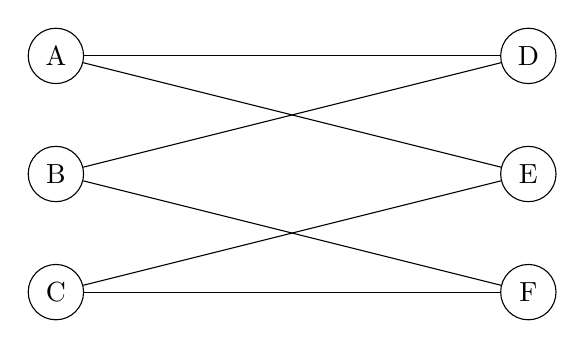
\begin{tikzpicture}[scale=1.5]
    \tikzset{vertex/.style = {shape=circle,draw,minimum size=2em}}
    \tikzset{edge/.style = {-,> = latex'}}
    % vertices on the left
    \node[vertex] (a) at (0,1) {A};
    \node[vertex] (b) at (0,0) {B};
    \node[vertex] (c) at (0,-1) {C};
    % vertices on the right
    \node[vertex] (d) at (4,1) {D};
    \node[vertex] (e) at (4,0) {E};
    \node[vertex] (f) at (4,-1) {F};
    % edges
    \draw (a) to (d);
    \draw (a) to (e);
    \draw (b) to (d);
    \draw (b) to (f);
    \draw (c) to (e);
    \draw (c) to (f);
    \end{tikzpicture}
    \caption{Initial 3x3 bipartite graph for the Maximum Matching Problem.}
    \label{fig:ACObipartite_graph}
\end{figure}

\subsubsection*{Step 1: Initialization}
In the first step, we initialize pheromone levels for all edges. Let’s assume a small initial pheromone value $\tau_0$ for all edges (e.g., $\tau_0 = 1$) as seen in figure \ref{fig:Initialized_graph}.

\begin{figure}[t]
    \centering
    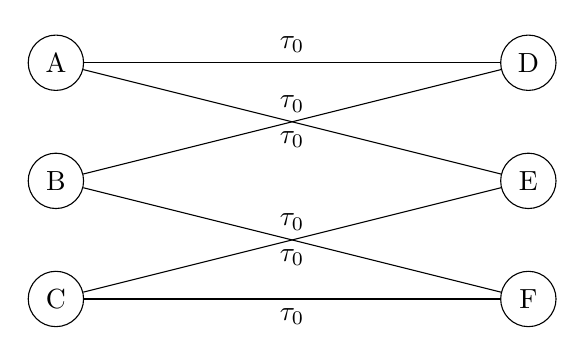
\begin{tikzpicture}[scale=1.5]
    \tikzset{vertex/.style = {shape=circle,draw,minimum size=2em}}
    \tikzset{edge/.style = {-,> = latex'}}
    % vertices on the left
    \node[vertex] (a) at (0,1) {A};
    \node[vertex] (b) at (0,0) {B};
    \node[vertex] (c) at (0,-1) {C};
    % vertices on the right
    \node[vertex] (d) at (4,1) {D};
    \node[vertex] (e) at (4,0) {E};
    \node[vertex] (f) at (4,-1) {F};
    % edges with pheromone values
    \draw (a) to node[midway, above] {$\tau_0$} (d);
    \draw (a) to node[midway, below] {$\tau_0$} (e);
    \draw (b) to node[midway, above] {$\tau_0$} (d);
    \draw (b) to node[midway, below] {$\tau_0$} (f);
    \draw (c) to node[midway, above] {$\tau_0$} (e);
    \draw (c) to node[midway, below] {$\tau_0$} (f);
    \end{tikzpicture}
    \caption{Graph with initialized pheromone values ($\tau_0$) on all edges.}
    \label{fig:Initialized_graph}
\end{figure}

\subsubsection*{Step 2: Ants Build Matchings}
Ants start to traverse the graph, selecting edges probabilistically based on pheromone values and a heuristic (e.g., choosing edges with available unmatched vertices). Each ant attempts to construct a matching.

In figure \ref{fig:Ant_selection} there are three ants, with Ant 1 starting from vertex A, Ant 2 from vertex B, and Ant 3 from vertex C.

\begin{figure}[t]
    \centering
    \begin{subfigure}[b]{0.3\textwidth}
        \centering
        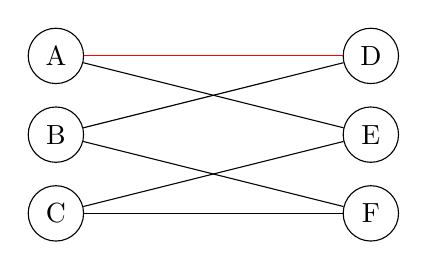
\begin{tikzpicture}
        \tikzset{vertex/.style = {shape=circle,draw,minimum size=2em}}
        \tikzset{edge/.style = {-,> = latex'}}
        % vertices on the left
        \node[vertex] (a) at (0,1) {A};
        \node[vertex] (b) at (0,0) {B};
        \node[vertex] (c) at (0,-1) {C};
        % vertices on the right
        \node[vertex] (d) at (4,1) {D};
        \node[vertex] (e) at (4,0) {E};
        \node[vertex] (f) at (4,-1) {F};
        % edges selected by Ant 1
        \draw[red] (a) to (d);
        \draw (a) to (e);
        \draw (b) to (d);
        \draw (b) to (f);
        \draw (c) to (e);
        \draw (c) to (f);
        \end{tikzpicture}
        \caption{Ant 1 selects edge (A, D).}
    \end{subfigure}
    \begin{subfigure}[b]{0.3\textwidth}
        \centering
        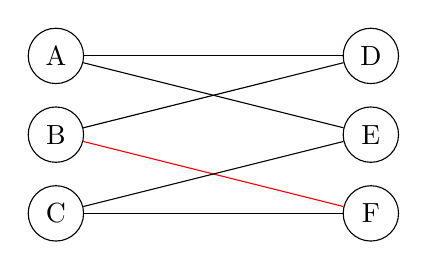
\begin{tikzpicture}
        \tikzset{vertex/.style = {shape=circle,draw,minimum size=2em}}
        \tikzset{edge/.style = {-,> = latex'}}
        % vertices on the left
        \node[vertex] (a) at (0,1) {A};
        \node[vertex] (b) at (0,0) {B};
        \node[vertex] (c) at (0,-1) {C};
        % vertices on the right
        \node[vertex] (d) at (4,1) {D};
        \node[vertex] (e) at (4,0) {E};
        \node[vertex] (f) at (4,-1) {F};
        % edges selected by Ant 2
        \draw (a) to (d);
        \draw (a) to (e);
        \draw[red] (b) to (f);
        \draw (b) to (d);
        \draw (c) to (e);
        \draw (c) to (f);
        \end{tikzpicture}
        \caption{Ant 2 selects edge (B, F).}
    \end{subfigure}
    \begin{subfigure}[b]{0.3\textwidth}
        \centering
        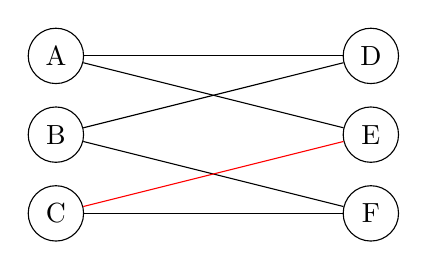
\begin{tikzpicture}
        \tikzset{vertex/.style = {shape=circle,draw,minimum size=2em}}
        \tikzset{edge/.style = {-,> = latex'}}
        % vertices on the left
        \node[vertex] (a) at (0,1) {A};
        \node[vertex] (b) at (0,0) {B};
        \node[vertex] (c) at (0,-1) {C};
        % vertices on the right
        \node[vertex] (d) at (4,1) {D};
        \node[vertex] (e) at (4,0) {E};
        \node[vertex] (f) at (4,-1) {F};
        % edges selected by Ant 3
        \draw (a) to (d);
        \draw (a) to (e);
        \draw (b) to (d);
        \draw (b) to (f);
        \draw[red] (c) to (e);
        \draw (c) to (f);
        \end{tikzpicture}
        \caption{Ant 3 selects edge (C, E).}
    \end{subfigure}
    \caption{Ants constructing matchings by selecting edges probabilistically.}
    \label{fig:Ant_selection}
\end{figure}

\subsubsection*{Step 3: Pheromone Update}
In figure \ref{fig:Pheromone_update} all ants have completed their matchings, and pheromones are updated. Pheromones on the edges selected by the ants are reinforced, while pheromones on other edges evaporate. Let $\Delta\tau$ represent the increase in pheromone for selected edges, and $\epsilon$ represent the evaporation factor.

\begin{figure}[t]
    \centering
    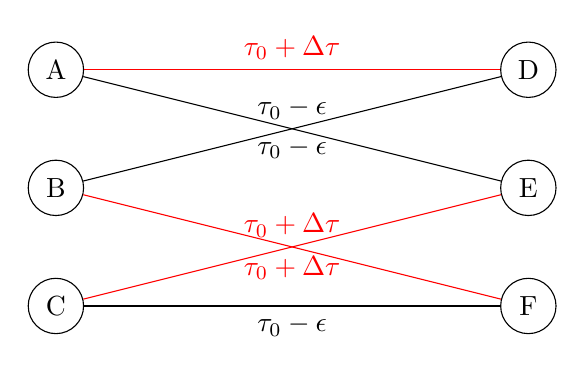
\begin{tikzpicture} [scale=1.5]
    \tikzset{vertex/.style = {shape=circle,draw,minimum size=2em}}
    \tikzset{edge/.style = {-,> = latex'}}
    % vertices on the left
    \node[vertex] (a) at (0,1) {A};
    \node[vertex] (b) at (0,0) {B};
    \node[vertex] (c) at (0,-1) {C};
    % vertices on the right
    \node[vertex] (d) at (4,1) {D};
    \node[vertex] (e) at (4,0) {E};
    \node[vertex] (f) at (4,-1) {F};
    % edges with pheromone updates
    \draw[red] (a) to node[midway, above] {$\tau_0 + \Delta\tau$} (d);
    \draw (a) to node[midway, below] {$\tau_0 - \epsilon$} (e);
    \draw[red] (b) to node[midway, above] {$\tau_0 + \Delta\tau$} (f);
    \draw (b) to node[midway, above] {$\tau_0 - \epsilon$} (d);
    \draw[red] (c) to node[midway, below] {$\tau_0 + \Delta\tau$} (e);
    \draw (c) to node[midway, below] {$\tau_0 - \epsilon$} (f);
    \end{tikzpicture}
    \caption{Pheromone update after constructing valid matchings.}
    \label{fig:Pheromone_update}
\end{figure}

\subsubsection*{Step 4: Repeat the Process (Multiple Iterations)}
The ants will repeat the process for a number of iterations, each time constructing matchings and updating the pheromone levels. The goal is to encourage the ants to explore edges that are part of high-quality matchings, while discouraging exploration of less optimal edges. Over time, the pheromone levels on better edges will accumulate, guiding future ants towards those edges.

For simplicity, let’s assume 3 iterations. After each iteration, pheromone values are updated, and ants select their next edges based on the updated pheromone levels.

\paragraph{Iteration 2 (After Updating Pheromone from Iteration 1):}
The ants will once again probabilistically select edges based on the pheromone levels, with a higher probability for edges that have been chosen frequently in the previous iteration (since they have higher pheromone levels).

In figure \ref{fig:ants2_selection} ant 1 selects a different edge based on the updated pheromone values:

\begin{figure}[t]
\centering
\begin{subfigure}[b]{0.3\textwidth}
\centering
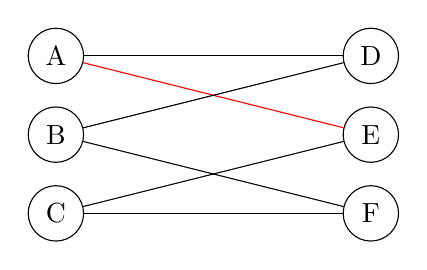
\begin{tikzpicture}
\tikzset{vertex/.style = {shape=circle,draw,minimum size=2em}}
\tikzset{edge/.style = {-,> = latex'}}
% vertices on the left
\node[vertex] (a) at (0,1) {A};
\node[vertex] (b) at (0,0) {B};
\node[vertex] (c) at (0,-1) {C};
% vertices on the right
\node[vertex] (d) at (4,1) {D};
\node[vertex] (e) at (4,0) {E};
\node[vertex] (f) at (4,-1) {F};
% edges selected by Ant 1 after pheromone update
\draw[red] (a) to (e); % Ant 1 switches to (A, E) after pheromone update
\draw (a) to (d);
\draw (b) to (d);
\draw (b) to (f);
\draw (c) to (e);
\draw (c) to (f);
\end{tikzpicture}
\caption{Ant 1 now selects edge (A, E).}
\end{subfigure}
\begin{subfigure}[b]{0.3\textwidth}
\centering
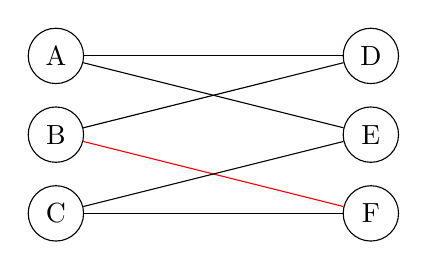
\begin{tikzpicture}
\tikzset{vertex/.style = {shape=circle,draw,minimum size=2em}}
\tikzset{edge/.style = {-,> = latex'}}
% vertices on the left
\node[vertex] (a) at (0,1) {A};
\node[vertex] (b) at (0,0) {B};
\node[vertex] (c) at (0,-1) {C};
% vertices on the right
\node[vertex] (d) at (4,1) {D};
\node[vertex] (e) at (4,0) {E};
\node[vertex] (f) at (4,-1) {F};
% edges selected by Ant 2 after pheromone update
\draw[red] (b) to (f); % Ant 2 sticks with (B, F)
\draw (a) to (d);
\draw (a) to (e);
\draw (b) to (d);
\draw (c) to (e);
\draw (c) to (f);
\end{tikzpicture}
\caption{Ant 2 sticks with edge (B, F).}
\end{subfigure}
\begin{subfigure}[b]{0.3\textwidth}
\centering
\begin{tikzpicture}
\tikzset{vertex/.style = {shape=circle,draw,minimum size=2em}}
\tikzset{edge/.style = {-,> = latex'}}
% vertices on the left
\node[vertex] (a) at (0,1) {A};
\node[vertex] (b) at (0,0) {B};
\node[vertex] (c) at (0,-1) {C};
% vertices on the right
\node[vertex] (d) at (4,1) {D};
\node[vertex] (e) at (4,0) {E};
\node[vertex] (f) at (4,-1) {F};
% edges selected by Ant 3 after pheromone update
\draw (c) to (f); 
\draw (a) to (d);
\draw (a) to (e);
\draw (b) to (d);
\draw (b) to (f);
\draw[red] (c) to (e);
\end{tikzpicture}
\caption{Ant 3 sticks with edge (C, E).}
\end{subfigure}
\caption{Ants constructing failed matchings after pheromone update.}
\label{fig:ants2_selection}
\end{figure}

\subsubsection*{Step 5: Evaluating and Improving the Matchings}
After several iterations, the ants will converge towards the edges that form the best matching. The pheromone values on these edges will be much higher, guiding future ants toward these edges. At the end of the process, you can evaluate the total matching based on the pheromone values accumulated across iterations.

Let’s assume the following results after 3 iterations:

\begin{itemize}
  \item Ant 1 successfully matched A to D.
  \item Ant 2 matched B to F.
  \item Ant 3 matched C to E.
\end{itemize}

The total matching could be:

\begin{itemize}
  \item A - D
  \item B - F
  \item C - E
\end{itemize}

This is a maximum matching because each vertex on the left is matched with exactly one vertex on the right, and no more matchings can be made without violating the constraints of the bipartite graph.

\subsubsection*{Step 6: Final Pheromone Adjustment and Conclusion}
In the final step, pheromones are updated again, ensuring that the best edges (those contributing to the maximum matching) are reinforced. Ants now have a high probability of selecting these edges in future iterations, and the algorithm converges to the optimal or near-optimal solution.

In this case, the matching A - D, B - F, and C - E is likely the optimal solution, which the algorithm has successfully found after several iterations of pheromone updates and edge selections.

\paragraph{}This example illustrates how the Ant Colony Optimization (ACO) algorithm can be adapted to solve the Maximum Matching Problem in bipartite graphs. The key steps of the process—edge selection based on pheromones, iterative construction of matchings, and pheromone updates—guide the ants toward an optimal solution. Through repeated iterations, the algorithm efficiently converges towards the maximum matching.




\subsubsection*{Ant Colony Optimization for NP Problems}
Ant Colony Optimization (ACO) has been widely applied to NP-hard problems due to its ability to find approximate solutions in complex search spaces. Among these problems, subset problems—where the goal is to find a subset of items that maximizes or minimizes a certain objective—are particularly significant. This section explores how ACO has been adapted for four well-known subset problems: the Traveling Salesman Problem (TSP), the Knapsack Problem, the Set Covering Problem, and the Independent Set Problem.

\paragraph{Traveling Salesman Problem (TSP):}
The Traveling Salesman Problem (TSP) is one of the most extensively studied NP-hard problems in combinatorial optimization. It requires finding the shortest possible route that visits a given set of cities exactly once and returns to the starting point. TSP is central in various fields, including logistics, routing, and manufacturing, where minimizing travel costs or time is essential. Despite its simple formulation, the computational complexity of TSP arises from the exponential growth in possible routes as the number of cities increases, making it impractical to solve through brute force methods for larger instances.

Ant Colony Optimization (ACO) was first successfully applied to the TSP by Dorigo et al. \cite{Dorigo2004}. Each ant in this system represents a potential solution, or route, and the algorithm mimics how real ants use pheromone trails to mark favorable paths. In the ACO for TSP, pheromones guide the selection of cities to visit, with shorter, more optimal routes receiving stronger pheromone reinforcement. This process of iterative pheromone updates allows the algorithm to increasingly favor better routes over time. Notably, the method was effective in discovering near-optimal solutions, particularly in cases where traditional heuristics like the nearest-neighbor approach were less efficient.

Later work by Leguizamon and Michalewicz \cite{Leguizamon1999} extended ACO's application to TSP by proposing a new version of the ant system specifically tailored to handle larger problem instances. Their approach emphasized balancing the exploration of new routes with the exploitation of known good solutions, a critical factor in ensuring that the algorithm did not prematurely converge on suboptimal routes. By introducing new mechanisms to control pheromone decay and deposit rates, their version of the ant system was able to maintain diversity in the search space while ensuring that promising routes were reinforced.

In evaluating the effectiveness of ACO on the TSP, both Dorigo and Leguizamon used benchmark datasets such as the TSPLIB to assess solution quality and computational efficiency. Metrics like the average tour length, computational time, and convergence rate were compared against established heuristics, such as the nearest-neighbor and genetic algorithms. In multiple cases, ACO demonstrated superior performance, particularly in terms of finding shorter routes and exhibiting robustness on larger, more complex instances of TSP. The ability to balance exploration and exploitation allowed ACO to outperform traditional approaches under certain conditions, especially as the problem size increased \cite{Stutzle2011}.

The adaptive nature of ACO made it particularly effective in solving TSP. By adjusting the algorithm’s parameters—such as the rate of pheromone evaporation and the amount of pheromone deposited—researchers could fine-tune the balance between intensification (exploiting known good routes) and diversification (exploring new ones). This flexibility enabled ACO to scale effectively and tackle larger instances of the problem, where other methods typically failed or required excessive computational resources.


\paragraph{Knapsack Problem:}
The Knapsack Problem is a classic NP-complete combinatorial optimization problem where the objective is to choose a subset of items, each with a specific weight and value, such that the total value is maximized without exceeding the weight capacity of a knapsack. This problem is central in fields like resource allocation, budgeting, and decision-making where a trade-off between constraints (e.g., weight) and rewards (e.g., value) needs to be balanced. Due to its computational complexity, exact algorithms often become impractical for large instances, making heuristic approaches like Ant Colony Optimization (ACO) an appealing alternative.

ACO can be adapted to solve the Knapsack Problem by viewing item selection as a path-building process, where each ant represents a candidate solution (a subset of items). In this context, the pheromone trails are used to guide the selection of items based on their value-to-weight ratio. As ants explore various item combinations, they reinforce those combinations that lead to higher total values without exceeding the knapsack's capacity. Pheromone updates play a crucial role in this iterative process, encouraging future ants to choose item combinations that have been proven successful by earlier ants.

Thomas Stützle describes how ACO can be applied to the Knapsack Problem by incorporating pheromone updates based on the quality of the solutions\cite{Stutzle2011}. In this approach, ants explore different subsets of items, and those that produce higher values within the given capacity constraints are reinforced. This reinforcement leads to a more informed search in future iterations, progressively guiding the ants towards optimal or near-optimal solutions. The algorithm’s adaptive nature allows it to dynamically adjust its search strategy based on the performance of past solutions, making it well-suited for tackling the inherent complexity of the Knapsack Problem.

In addition to the basic ACO framework, hybrid approaches have been developed to further improve solution quality for the Knapsack Problem. For instance, combining ACO with local search techniques, such as dynamic programming or greedy algorithms, enhances the algorithm's performance, particularly when dealing with large item sets or complex constraints. These hybrid methods allow ACO to refine its solutions by exploiting the strengths of local search to intensify the search in promising areas of the solution space, while maintaining ACO's exploratory capabilities. This combination often leads to better results than using ACO or traditional methods in isolation, especially in complex, large-scale instances \cite{Stutzle2011}.

Evaluations of ACO's effectiveness on the Knapsack Problem are typically conducted using benchmark instances. Key performance metrics include solution quality (the total value of selected items), computational efficiency, and the ability to scale to larger problem instances. Comparative studies have demonstrated that ACO, especially when hybridized with local search techniques, can outperform traditional methods in terms of finding high-quality solutions within reasonable computational timeframes, particularly when exact algorithms become infeasible for larger datasets.

\paragraph{Set Covering Problem (SCP)}
The Set Covering Problem (SCP) is a classic NP-complete problem that requires finding the smallest subset of sets whose union covers all elements in a given universal set. SCP appears in a wide variety of practical applications, such as resource allocation, network design, facility location, and scheduling. The challenge with SCP is its combinatorial explosion: as the number of sets grows, the number of possible combinations increases exponentially. This makes exact solutions computationally expensive, particularly for large-scale instances.

Ant Colony Optimization (ACO) is an effective method for tackling SCP, as it excels in exploring large solution spaces and can dynamically adapt to the problem’s constraints. In ACO's application to SCP, each ant incrementally builds a solution by selecting sets to include, aiming to cover all elements in the universal set. Pheromones deposited on sets guide the ants in future iterations, encouraging the selection of sets that have historically been part of good solutions.

Ankit Pat enhanced the ACO algorithm for SCP by adapting the pheromone update mechanism\cite{Pat2014}. In this variant, ants are rewarded for selecting sets that either cover more elements or contribute to smaller overall solutions. The pheromone levels are adjusted after each iteration to reflect the quality of the solution, favoring sets that help achieve a complete cover with minimal redundancy. This approach allows the algorithm to focus on sets that are frequently part of optimal or near-optimal solutions, gradually improving the quality of the solution with each cycle \cite{Pat2014}.

The primary computational difficulty in SCP lies in evaluating all possible combinations of sets, especially as the problem size increases. Traditional approaches, such as greedy algorithms, attempt to build solutions quickly but often result in suboptimal results due to their myopic nature. Exact methods, such as branch-and-bound or integer programming, provide optimal solutions but become computationally prohibitive for large instances.

ACO addresses this by balancing exploration and exploitation through the use of pheromone trails and heuristic information. Ants explore a wide range of solutions by probabilistically selecting sets based on their pheromone levels and the heuristic value (e.g., how many uncovered elements a set includes). This enables ACO to effectively navigate large solution spaces and avoid local optima.

The effectiveness of ACO in solving SCP has been evaluated on standard benchmark instances, comparing it to both greedy heuristics and exact algorithms. Studies, including those by Marco Dorigo and Ankit Pat, have shown that ACO is highly competitive, particularly on large-scale problems where exact methods are impractical due to time constraints\cite{Pat2014,Dorigo2004}. For example, on datasets with hundreds of sets and elements, ACO was able to find near-optimal solutions in a fraction of the time required by exact methods.

Guillermo Leguizamon and Zbigniew Michalewicz demonstrated that their ACO variant for SCP consistently produced better solutions than traditional heuristic methods\cite{Leguizamon1999}. The results indicated that ACO outperformed the greedy algorithm by finding smaller set covers, especially in instances where the greedy approach failed to adequately balance the coverage of elements with the size of the solution \cite{Leguizamon1999}.

The evaluation metrics typically focus on the size of the solution (i.e., the number of sets selected) and the computational time. ACO has been shown to provide a good balance between solution quality and computational efficiency, making it a viable option for large SCP instances where exact methods are infeasible.

\paragraph{Independent Set Problem (ISP)}
The Independent Set Problem (ISP) is an NP-hard problem where the objective is to find the largest subset of vertices in a graph such that no two vertices in the subset are adjacent. ISP has significant applications in fields like network theory, resource allocation, and scheduling, where minimizing conflicts or dependencies between resources is critical. The complexity of ISP stems from the difficulty of ensuring that no adjacent vertices are included in the independent set, especially in large and dense graphs.

ACO has been adapted to solve ISP by treating the problem as one of selecting a subset of non-adjacent vertices. Each ant explores the graph by adding vertices to its candidate solution while ensuring that the adjacency constraints are respected. Pheromone trails are laid on vertices that lead to larger independent sets, guiding future ants toward promising areas of the solution space.

The challenge in ISP is evaluating the potential inclusion of vertices in a way that respects the adjacency constraints while attempting to maximize the size of the independent set. Greedy algorithms tend to struggle with this problem because they often make short-sighted decisions that lead to suboptimal solutions. Exact methods, such as dynamic programming or backtracking, guarantee optimal solutions but are computationally expensive and impractical for large graphs.

ACO’s approach to ISP involves constructing solutions iteratively, with ants making probabilistic decisions based on pheromone levels and heuristic information. The heuristic typically estimates the benefit of including a vertex, considering both the size of the current independent set and the adjacency constraints. As ants traverse the graph, they reinforce the selection of vertices that have been part of larger independent sets in previous iterations.

The performance of ACO in solving ISP has been evaluated in comparison with both greedy algorithms and exact methods. ACO tends to outperform greedy algorithms, particularly on larger graphs where the problem's complexity increases. Ankit Pat and Thomas Stützle showed that ACO could find significantly larger independent sets than traditional algorithms, especially in dense graphs where the adjacency constraints are more restrictive \cite{Pat2014,Stutzle2011}.

In terms of solution quality, ACO is competitive with exact methods but requires significantly less computational time. For instance, Ankit Pat applied ACO to a variety of graph instances, demonstrating that the algorithm consistently found near-optimal solutions\cite{Pat2014}. The size of the independent set discovered by ACO was often close to the best-known solutions, and in some cases, ACO even matched the performance of exact methods, but with much greater efficiency.

Additionally, hybrid ACO algorithms that incorporate local search techniques have been shown to further enhance the performance of ACO in solving ISP. By refining solutions through small modifications, such as adding or removing a vertex, hybrid approaches can explore a wider range of potential solutions, leading to even larger independent sets in complex graph instances. Hung-Pin Shih highlighted that these hybrid techniques are especially effective when dealing with weighted versions of ISP, where the goal is to maximize the total weight of the selected vertices, not just the size of the set \cite{Shih2008}.

\paragraph{Subset Problems in Other Domains}
Beyond the traditional NP-hard problems, Ant Colony Optimization (ACO) has been successfully applied to a wide range of subset problems across various domains. These applications demonstrate the adaptability and versatility of ACO in tackling diverse optimization challenges by customizing its pheromone update rules and heuristic strategies according to the specific characteristics of each domain.

In network design, ACO has been used to optimize the selection of links in communication networks. The objective is to select a subset of links that minimizes the cost while maintaining connectivity across the network. ACO's flexibility allows it to explore different configurations of network links, and its pheromone update mechanism guides the algorithm towards selecting those links that lead to more efficient and cost-effective network structures. This ability to handle dynamic and complex networks makes ACO an appealing approach for real-world network design problems, especially those involving large and complex network topologies \cite{Dorigo2004}.

In bioinformatics, ACO has been applied to subset selection problems such as selecting genes or proteins relevant to certain biological processes or diseases. The challenge here is to identify the most informative subset of features (such as genes) from a larger set that contribute to accurate predictions or classifications. ACO adapts to bioinformatics problems by using pheromone updates based on the relevance of genes or proteins in the context of a given biological dataset. By doing so, the algorithm can efficiently identify subsets of genes or proteins that maximize predictive accuracy or classification performance, while avoiding overfitting or computational inefficiency \cite{Stutzle2011}.

These diverse applications underscore the broad utility of ACO in solving subset problems across different fields. The ability to dynamically adjust pheromone updates, combined with tailored heuristic strategies for each specific problem, allows ACO to find high-quality solutions in domains as varied as network design and bioinformatics. This adaptability has made ACO a powerful tool for tackling complex subset problems where traditional methods might struggle or fail to provide satisfactory results \cite{Leguizamon1999}.



\paragraph{}In each of these applications, the fundamental mechanism of ACO—building solutions incrementally while reinforcing high-quality components—proves highly effective for subset problems, which often involve large solution spaces and complex constraints.

\subsubsection*{Results and Performance Comparison}
Through extensive research, we have found that Ant Colony Optimization (ACO) has shown significant efficiency in solving various NP-hard problems, such as the Traveling Salesman Problem (TSP), Job Scheduling, and Graph Coloring. These problems, like Maximum Matching, involve large solution spaces and complex optimization criteria, making them difficult to solve efficiently with traditional methods. The adaptability of ACO in these contexts suggests that it could similarly offer an efficient approach to the Maximum Matching problem, particularly in larger and more complex graphs.

The strength of ACO lies in its ability to explore and exploit the search space in a way that balances the trade-off between finding new, potentially better solutions (exploration) and refining known solutions (exploitation). This dynamic nature of the algorithm, combined with its distributed, population-based approach, enables it to handle complex combinatorial optimization problems effectively, even when the solution space grows exponentially. The ability to adaptively update pheromones allows ACO to avoid getting trapped in local minima, a common issue with many traditional optimization methods.

Given these successes in other NP-hard problems, we believe ACO holds strong potential for addressing the Maximum Matching problem. The next logical step in our work is to implement the ACO algorithm, not only for bipartite graphs but also for more graph structures, including d-partite and general graphs. By extending ACO to these broader contexts, we can evaluate its scalability and effectiveness in even more complex matching scenarios. the aim to explore how the algorithm can be tailored to account for the additional complexity introduced by multi-partite and non-bipartite structures. This would involve refining the pheromone update mechanism and ensuring that the algorithm can efficiently handle the diverse constraints and relationships within such graphs. By doing so, we hope to extend the applicability of ACO to a wider range of combinatorial optimization problems, further demonstrating its potential as an efficient solution method for large-scale, complex matching problems.


\subsubsection*{Conclusion}
In conclusion, ACO presents a promising approach to solving the Maximum Matching Problem in bipartite graphs, particularly when scalability is a concern. By adapting the pheromone update rules and integrating local search techniques, ACO can offer a competitive alternative to exact methods for large instances.




\subsection{Karp-Sipser}
\label{subsec:karp_sipser}
% Author: Ryan Feneley, IN-PROGRESS, Reviewer: Ethan K, Due Date: 11/19

The Karp-Sipser Algorithm, introduced in 1981, provides a heuristic-based solution to the problem of finding large matchings in graphs, with particular success in sparse random graph structures. Unlike exact algorithms, which guarantee optimality but often at significant computational expense, the Karp-Sipser approach is focused on efficiency. Its design combines strategic vertex selection with randomness to achieve matchings that are asymptotically close to maximum. The algorithm operates with a time complexity of \(O(n + m)\), where \(n\) is the number of vertices and \(m\) is the number of edges, making it particularly well-suited to large, sparse graphs \cite{aronson1997maximum}.

\paragraph{Algorithm Mechanism}
The Karp-Sipser algorithm employs a two-phase process to build a large matching while maintaining computational simplicity:
\begin{enumerate}
    \item Targeted Greedy Matching:
    The first phase capitalizes on pendant vertices—vertices with a degree of one. These vertices are inherently simple to match, as they have only one neighbor. By immediately adding these vertices and their neighbors to the matching, the algorithm ensures that these straightforward cases are resolved early. The removal of matched vertices and their adjacent edges reduces the graph’s complexity, setting the stage for more nuanced decisions in the second phase.
    
    \item Randomized Matching:
    Once no pendant vertices remain, the algorithm switches to a random edge selection strategy. Edges are selected randomly from the remaining graph, and their endpoints are added to the matching. This phase continues iteratively, with matched vertices being removed after each selection, until the graph is fully processed or no more matchable edges remain.
\end{enumerate}

This two-step combination of deterministic and probabilistic methods allows the Karp-Sipser algorithm to adapt dynamically to the structure of the graph, leveraging its simplicity in sparse cases and flexibility in more complex scenarios.

\paragraph{Efficiency and Practical Performance}
The Karp-Sipser algorithm stands out for its linear time complexity, \(O(n + m)\), making it one of the fastest heuristic methods for graph matching. This efficiency is achieved by focusing on pendant vertices in the initial phase, a strategy that simplifies the graph and reduces computational overhead. In sparse random graphs, the algorithm performs exceptionally well, producing matchings that are nearly maximal in most cases. The targeted matching of pendant vertices ensures that the most straightforward edges are resolved first, leaving a smaller, more manageable subgraph for the random selection phase.

\paragraph{Insights from Revisited Analysis}
A detailed analysis in 1997, titled "Maximum Matchings in Sparse Random Graphs: Karp-Sipser Revisited," provided a deeper understanding of the algorithm’s performance across different graph structures \cite{aronson1997maximum}. The study confirmed that the algorithm’s effectiveness is highly dependent on graph sparsity. For graphs with an average vertex degree less than \(e \approx 2.718\), the Karp-Sipser algorithm consistently produces matchings that are close to the maximum. This finding reinforced its utility as a practical alternative to exact algorithms in scenarios where computational resources are limited.

The analysis also highlighted the diminishing returns of the algorithm in dense graphs. Here, the random edge selection phase can result in suboptimal matchings due to the lack of clear pendant vertices. Despite this, the study demonstrated the algorithm’s robustness in sparse environments, where its heuristic nature is well-aligned with the problem structure.

\paragraph{Applications}
The Karp-Sipser algorithm’s blend of simplicity and speed has enabled its use in a variety of applications:
\begin{itemize}
    \item Random Graph Analysis:
    Frequently employed in the study of Erdős–Rényi random graphs, the algorithm provides insights into the properties of large graph structures.
    \item Approximation Frameworks:
    Serves as a foundational tool in approximation schemes for problems that do not require exact matchings.
    \item Preprocessing for Exact Algorithms:
    The greedy phase of Karp-Sipser can act as a preprocessing step to simplify input graphs before applying more computationally intensive methods.
    \item Real-Time Decision Systems:
    Its low computational cost makes it a viable choice for real-time applications where approximate solutions suffice, such as task allocation or resource matching in distributed systems.
\end{itemize}

\paragraph{Strengths and Weaknesses}
The primary strength of the Karp-Sipser algorithm lies in its ability to balance speed with solution quality, particularly in sparse graph settings. Its targeted approach to pendant vertices ensures that the algorithm efficiently handles cases where a large proportion of vertices have low degrees. Furthermore, its random phase adds flexibility, allowing it to operate effectively even in graphs with less predictable structures.

However, the algorithm’s reliance on pendant vertices means it performs less effectively in dense graphs, where such vertices are rare or nonexistent. In these cases, the random selection phase dominates, often leading to suboptimal matchings. This limitation contrasts sharply with exact methods, such as Edmonds' Blossom Algorithm, which are designed to handle complex structures more systematically.

\paragraph{Impact and Legacy}
The Karp-Sipser algorithm has been a cornerstone for heuristic approaches to matching problems. Its design has influenced the development of other approximate and hybrid algorithms, particularly those aimed at balancing computational efficiency with solution quality. While it is not a universal solution, itis a vital component of the graph algorithm toolkit.

\paragraph{Conclusion}
The Karp-Sipser algorithm is a prime example of how heuristic methods can achieve a balance between computational efficiency and practical applicability. Its emphasis on leveraging graph structure—particularly pendant vertices—sets it apart as a specialized tool for sparse random graphs. While it does not guarantee optimal solutions, its low complexity and strong performance in appropriate contexts ensure its continued relevance in both theoretical research and practical applications.


\subsection{Auction Algorithm}
\label{subsec:auction}
% Author: Ryan Feneley, IN-PROGRESS, Reviewer: Ethan K, Due Date: 11/19
\subsection*{Auction Algorithm (1981)}

The Auction Algorithm, introduced by Dimitri Bertsekas in 1981, is an iterative method designed to solve the maximum weighted matching problem. Inspired by the dynamics of auctions, the algorithm operates by associating prices with vertices and iteratively refining these prices to maximize the total weight of the matching \cite{bertsekas1981auction}. It is particularly effective for solving large-scale assignment problems and has found applications in various domains due to its scalability and simplicity.

\paragraph{Algorithm Mechanism}
The Auction Algorithm relies on a bidding and assignment process to allocate vertices optimally. Its key steps are:
\begin{enumerate}
    \item Initialization: Each vertex in one partition of the graph is initially unassigned, and all prices are set to zero.
    \item Bidding Phase: Each unassigned vertex determines the edge with the highest "profit," which is defined as the weight of the edge minus the price of the connected vertex in the other partition. The vertex bids an increment over the current highest price to secure this edge.
    \item Assignment Phase: Vertices in the other partition accept the highest bid, updating their assignments and prices accordingly.
    \item Iterative Refinement: The process repeats until all vertices are assigned or a predefined termination criterion is met.
\end{enumerate}

This auction-based mechanism ensures that vertices compete for assignment, driving the solution toward an optimal matching.

\paragraph{Performance and Complexity}
The Auction Algorithm achieves a time complexity of \(O(n^2 \log n)\), where \(n\) is the number of vertices in the graph. This performance makes it highly efficient for dense graphs and large-scale problems. Furthermore, its decentralized nature allows for parallelization, which can significantly speed up computations in distributed systems.


\paragraph{Strengths and Limitations}
The primary strength of the Auction Algorithm lies in its simplicity and scalability. Its iterative approach is well-suited to parallel computation, making it efficient for large datasets. However, the algorithm may face challenges in sparse graphs where competition for edges is limited, leading to slower convergence. Additionally, while the algorithm guarantees optimal solutions in weighted bipartite graphs, its extension to non-bipartite settings requires significant adaptation.

\paragraph{Conclusion}
The Auction Algorithm remains a cornerstone in the study of maximum weighted matching problems. Its ability to balance computational efficiency with solution quality has made it a staple in both theoretical research and practical applications. By leveraging market-inspired dynamics, it offers a unique approach to optimization that continues to influence the development of advanced algorithms in combinatorial optimization.


\subsection{A* Algorithm}
\label{subsec:A_star}
% Author @ Jeremy Perez, UNDER-REVIEW, Reviewer @ Claudia Porto

A* is a much more sophisticated graph traversing algorithm capable of finding the shortest path between two nodes. Before formally defining it, there exists some additional concepts which prove to be important when understanding it's adoption in this study.

\subsubsection{Problem Modeling}

Any problem can be modeled by formally defining the following:
\begin{enumerate}
    \item \textbf{Initial States}: What initial state can an algorithm begin with?
    \item \textbf{Possible actions}: What \textbf{actions} can be taken given the current state?
    \item \textbf{Successor Function} What state is an algorithm in after it performs an action?
    \item \textbf{Goal Test}: Is the current state the goal state of the problem?
\end{enumerate}

\noindent This formulation is commonly defined using the notion of an \textit{agent} but for the sake of conciseness, we have restricted its definition to mean just algorithm, given the fact that we'll be formulating problems for algorithms to solve.



\subsubsection{State Spaces}
A \textbf{state space} is a structure that represents all possible configurations of a problem. Formally it is defined using a tuple $(N,E,S,G)$ where:

\begin{itemize}
    \item $N$ is the set of states.
    \item $E$ is the set of directed edges connecting states.
    \item $S \subseteq N$ is a nonempty set that contains the starting states.
    \item $G \subseteq N$ is a nonempty set that contains a goal state.
\end{itemize}

\noindent
These structures can be quite useful for testing decision-making strategies on a problem.

Let's work through a concrete example. Suppose you are getting ready for work and you notice that you are barefoot. You task yourself with putting on a single shoe first. If we were to observe the state space of putting on a shoe, we get that:
\begin{itemize}
    \item $N =$ \{bareFoot, sockOnFoot, shoeOn\})
    \item $E =$ \{(bareFoot, sockOnFoot), (sockOnFoot,bareFoot), (sockOnFoot,shoeOn), (shoeOn,sockOnFoot)\})
    \item $S =$ \{bareFoot\}
    \item $G =$ \{shoeOn\}
\end{itemize}

\begin{center}
\begin{tikzpicture}[scale=1.5]
    % Draw nodes for V1
    \node[ultra thick ,double, minimum size=1.5cm, draw,label=above:{Inital}] (1) at (0, 0) {bareFoot};
    \node[ultra thick,minimum size=1.5cm, draw] (2) at (3, 0) {sockOnFoot};
    \node[ultra thick,minimum size=1.5cm, draw,label=above:{Goal}] (3) at (6, 0) {shoeOn};

    % Draw edges
    \draw[ultra thick, <->] (1) -- (2) ;
    \draw[ultra thick, <->] (2) -- (3);
\end{tikzpicture}
\end{center}
\noindent
Notice that in this example, you are not able to directly go from being bareFoot to a state of being with a shoeOn. 
It requires going to a state of sockOnFoot first. By design, this 
model embeds every action possible
at any given time. It essentially is capable of making any decision-based problem into a graph problem.

\subsubsection{Problem Modeling of Maximum Matching}
Applying these concepts to the Maximum Matching problem, let us begin by observing what some formulations of this problem look like. Usually, the largest difference between Maximum Matching formulations is the representation of states. Because of the existence of reductive solutions, formulations can vary greatly. Here are some simple ones:
\begin{itemize}
    \item \textbf{Subset Formulation}: Assume you begin with the graph $G=(V,E)$ where $V$ denotes the set of vertices and $E$ denotes the set of edges.
Suppose your initial state is the entire edge-set $E$.
Let the possible actions at any state be removing any of the edges in the current edge set of the state. Let the successor function remove the edge out of the set. 
The goal test is whether or not the current state's edge set is a maximum matching of $G$. 
\item \textbf{Superset Formulation}: Assume you begin with the graph $G=(V,E)$ where $V$ denotes the set of vertices and $E$ denotes the set of edges, suppose your initial state's edge-set is the empty set $\emptyset$.
Let the possible actions at any state add an edge from $E$ which is not currently present in the edge set. Let the successor function add the chosen edge to the edge set. 
The goal test is whether or not the current state's edge set is a maximum matching of $G$. 
\end{itemize}


\noindent Using Figure~\ref{fig:subsetStates} to visualize the structure of a Max Matching State Space, we uncover that there exists some underlying mathematical relationships to these types of structures. The states in this space directly correspond to the elements of the \textbf{Power Set} of $E$, denoted $\mathcal{P}(E)$, which is the set of all possible subsets of a set. This set has a cardinality of $2^{|E|}$.

Notice that the Superset formulation can be articulated by flipping the goal and initial states and flipping the direction of every transition in the state space of the Subset formulation. These formulation directly relates to power sets being \textit{Boolean algebras} under normal set operations and boolean algebras having a \textit{dual}. This explains why the state space forms a lattice-like structure. Useful properties of these mathematical structures may prove to be helpful at developing refined renditions of this problem.

\begin{figure}
\centering
\begin{tikzpicture}[
node distance = 15mm and 20mm,
  start chain = going right,
     N/.style = {inner sep=1pt, on chain,minimum size=1cm, draw},
                    ]
\node (n21) [N] {...};
\node (n22) [N] {...};
\node (n23) [N] {...};
\node (n24) [N] {...};
\node (n25) [N] {...};
%
\node (n11) [N, label=left:{Removed Edges: $m-1$}, below=of n21]           {$\{e_m\}$};
\node (n12) [N, below=of n22] {$\{e_{m-1}\}$};
\node (n13) [N, below=of n23]{$...$};
\node (n14) [N, below=of n24] {$\{2\}$};
\node (n15) [N, below=of n25] {$\{1\}$};
%
\draw [<-](n11) -- (n21);
\draw [<-](n11) -- (n22);
\draw [<-](n11) -- (n23);
\draw [<-](n11) -- (n24);
\draw [<-](n11) -- (n24);
\draw [<-](n11) -- (n25);
\draw [<-](n12) -- (n21);
\draw [<-](n12) -- (n22);
\draw [<-](n12) -- (n23);
\draw [<-](n12) -- (n24);
\draw [<-](n12) -- (n24);
\draw [<-](n12) -- (n25);
\draw [<-](n13) -- (n21);
\draw [<-](n13) -- (n22);
\draw [<-](n13) -- (n23);
\draw [<-](n13) -- (n24);
\draw [<-](n13) -- (n24);
\draw [<-](n13) -- (n25);
\draw [<-](n14) -- (n21);
\draw [<-](n14) -- (n22);
\draw [<-](n14) -- (n23);
\draw [<-](n14) -- (n24);
\draw [<-](n14) -- (n24);
\draw [<-](n14) -- (n25);
\draw [<-](n15) -- (n21);
\draw [<-](n15) -- (n22);
\draw [<-](n15) -- (n23);
\draw [<-](n15) -- (n24);
\draw [<-](n15) -- (n24);
\draw [<-](n15) -- (n25);
%
\node (n31) [N, label=left:{Removed Edges: 1}, above=of $(n21.south)!0.5!(n22.south)$]  {$\{e_2,e_3,...,e_m\}$};
\node (n32) [N, above=of n23]  {...};
\node (n33) [N, above=of $(n24.south)!0.5!(n25.south)$]  {$\{e_1,e_3,...,e_{m-1}\}$};
%
\draw [->](n31) -- (n21)    ;
\draw [->](n31) -- (n22)  ;
\draw [->](n31) -- (n23) ;
\draw [->](n31) -- (n24) ;
\draw [->](n31) -- (n25);
\draw [->](n32) -- (n21)    ;
\draw [->](n32) -- (n22)  ;
\draw [->](n32) -- (n23) ;
\draw [->](n32) -- (n24) ;
\draw [->](n32) -- (n25);
\draw [->](n33) -- (n21)    ;
\draw [->](n33) -- (n22)  ;
\draw [->](n33) -- (n23) ;
\draw [->](n33) -- (n24) ;
\draw [->](n33) -- (n25);
;
%
\node (n41) [N, double, label=above:{Inital}, above=of $(n32.north)$] {$\{e_1,e_2,...,e_m\}$};
%
\draw [->](n41) -- (n31);  
\draw [->](n41) -- (n32);
\draw [->](n41) -- (n33);
%
\node (n51) [N, below=of n13] {$\emptyset$};
%
\draw [<-](n51) -- (n11);
\draw [<-](n51) -- (n12);
\draw [<-](n51) -- (n13);
\draw [<-](n51) -- (n14);
\draw [<-](n51) -- (n15);
\end{tikzpicture}
\caption{This is a visualization of the state space of a Maximum Matching problem using the Subset Formulation.}
\label{fig:subsetStates}

\end{figure}






\subsubsection{Optimizing State Spaces}
As foreshadowed, it is possible to truncate state spaces for the sake of optimizing traversal strategies. For instance, using the fact that the maximum matching is always $n$ (the number of vertices) or less means a new problem formulation of the problem can be made by removing all states where the edge-set is bigger than $n$. The resulting state space would then have initial states starting with edge sets with $n$ elements. Applying this to the subset formulation of maximum matching, we would get a smaller subspace that looks like Figure~\ref{fig:truncatedStates}

\begin{figure}
    \centering
    
\begin{tikzpicture}[
node distance = 10mm and 5mm,
  start chain = going right,
     N/.style = {inner sep=1pt, on chain,minimum size=1cm, draw},
                    ]
\node (n21) [N] {...};
\node (n22) [N] {...};
\node (n23) [N] {...};
\node (n24) [N] {...};
\node (n25) [N] {...};
%
\node (n11) [N, label=left:{Removed Edges: $m-1$}, below=of n21]           {$\{e_m\}$};
\node (n12) [N, below=of n22] {$\{e_{m-1}\}$};
\node (n13) [N, below=of n23]{$...$};
\node (n14) [N, below=of n24] {$\{2\}$};
\node (n15) [N, below=of n25] {$\{1\}$};
%
\draw [<-](n11) -- (n21);
\draw [<-](n11) -- (n22);
\draw [<-](n11) -- (n23);
\draw [<-](n11) -- (n24);
\draw [<-](n11) -- (n24);
\draw [<-](n11) -- (n25);
\draw [<-](n12) -- (n21);
\draw [<-](n12) -- (n22);
\draw [<-](n12) -- (n23);
\draw [<-](n12) -- (n24);
\draw [<-](n12) -- (n24);
\draw [<-](n12) -- (n25);
\draw [<-](n13) -- (n21);
\draw [<-](n13) -- (n22);
\draw [<-](n13) -- (n23);
\draw [<-](n13) -- (n24);
\draw [<-](n13) -- (n24);
\draw [<-](n13) -- (n25);
\draw [<-](n14) -- (n21);
\draw [<-](n14) -- (n22);
\draw [<-](n14) -- (n23);
\draw [<-](n14) -- (n24);
\draw [<-](n14) -- (n24);
\draw [<-](n14) -- (n25);
\draw [<-](n15) -- (n21);
\draw [<-](n15) -- (n22);
\draw [<-](n15) -- (n23);
\draw [<-](n15) -- (n24);
\draw [<-](n15) -- (n24);
\draw [<-](n15) -- (n25);
%
\node (n31) [N, label=above:{Initial},label=left:{Removed Edges: $(m-n)$}, above=of n21]  {$\{e_1,e_2,...,e_n\}$};
\node (n32) [N, label=above:{Initial},above=of $(n23.north)$]  {...};
\node (n33) [N, label=above:{Initial},label=right:{\# of States in Level $= \binom{m}{n}$ },above=of n25]  {$\{e_{m-n},e_{m-n+1},...,e_{m}\}$};
%
\draw [->](n31) -- (n21)    ;
\draw [->](n31) -- (n22)  ;
\draw [->](n31) -- (n23) ;
\draw [->](n31) -- (n24) ;
\draw [->](n31) -- (n25);
\draw [->](n32) -- (n21)    ;
\draw [->](n32) -- (n22)  ;
\draw [->](n32) -- (n23) ;
\draw [->](n32) -- (n24) ;
\draw [->](n32) -- (n25);
\draw [->](n33) -- (n21)    ;
\draw [->](n33) -- (n22)  ;
\draw [->](n33) -- (n23) ;
\draw [->](n33) -- (n24) ;
\draw [->](n33) -- (n25);
;

%
\node (n51) [N, below=of n13] {$\emptyset$};
%
\draw [<-](n51) -- (n11);
\draw [<-](n51) -- (n12);
\draw [<-](n51) -- (n13);
\draw [<-](n51) -- (n14);
\draw [<-](n51) -- (n15);
\end{tikzpicture}


    \caption{Truncated version of Figure~\ref{fig:subsetStates} where the first $m-n-1$ levels were removed and each proceeding leaf state from it's bottom most level has become initial states. }
    \label{fig:truncatedStates}
\end{figure}    


\subsubsection{Traversal Strategies to Find Solution States}

Strategies for traversing state spaces to find solutions (analogous to finding goal states) are broken into two major classifications: 
\begin{itemize}
    \item \textbf{Uninformed search} strategies refer to algorithms that traverse state spaces without any more information about states beyond what is specified in the problem. All that is known to these algorithms is whether or not a state is a goal state.  Examples of this include deploying Breadth First Search, Iterative deepening search, or Bidirectional Search on the state space to find solutions.
    \item \textbf{Informed search}, also known as \textbf{Heuristic search}, refers to algorithms that use additional information, beyond a problem formulation, to decide how to traverse state spaces. 
\end{itemize}

\noindent In the example of using breadth-first search, this is exactly what the un-pruned brute force algorithm is. Its runtime has a known worst-case running time of $O(2^m)$ and corresponds to the algorithm traversing through every state mentioned in the Subset Formulation of the problem. 


\subsubsection{Best-First Search and A*}

\textbf{Best-First} search is the most common form of informed search.
It utilizes an \textbf{evaluation function} to calculate a state's
\textit{costliness} and expands nodes that are the cheapest. Please refer to Figure~\ref{fig:BestFirst}
 to see a quick example.

The evaluation function estimates cost using various factors and is often a composition of functions.


One function commonly found inside the evaluation function is the heuristic component/function. A \textbf{heuristic function} given a state, calculates an estimated cheapest cost to the remaining distance to a goal state. A good way to think about this is that it's a value associated with the remaining "distance" to an answer. 


\begin{figure}
    \centering
    \begin{tikzpicture}[node distance=2.5cm, auto, scale=0.5]
    \node[ double, thick,circle, minimum size=1.5cm, draw] (S) at (0,0) {S};
    \node[ thick,circle, minimum size=1.5cm, draw] (A) [below of=S ] {A};
    \node[ thick,circle, minimum size=1.5cm, draw] (B) [ right of=S] {B };
    \node[ thick,circle, minimum size=1.5cm, draw] (C) [right of=A] {C };
    \node[ thick,circle, minimum size=1.5cm, draw] (D) [right of=B] {D};
    \node[ thick,circle, minimum size=1.5cm, draw] (G) [right of=C] {G};
    
    % Draw the edges
    \path[ultra thick, ->] 
  (S) edge node {2} 
  (A) edge node {4} (B)
  (A) edge node {2} (C)
  (B) edge node {2} (D)
  (C) edge node {1} (G)
  (D) edge node {3} (G);
    
\end{tikzpicture}
    \caption{Let's say we want to find some shortest path from a initial state $S$ to a goal state $G$ using a Best First Search algorithm. In an automaton style of execution, the cheapest action is to go to state $A$. Wholistically, the next cheapest action is to go to state $C$ and again the cheapest action from there is to go to $G$. The order of expansion would be $S,A,C,G$}
    \label{fig:BestFirst}
\end{figure}



\textbf{A* }is a type of Best-First Search Algorithm that traverses through a graph minimizing the total estimated cost. Its evaluation function is the combination of the cost to reach a node and the cost from the node to the goal. Since it's a best-first search algorithm, it's expanding states based upon the cheapest estimated cost of a path going through a state.


\subsubsection*{Optimal Heuristics}
Not all heuristics are equal and finding one which will give a good estimation of the remaining short distance to a goal state consistently can be challenging. An \textbf{admissible heuristic} is one that \textit{never overestimates} the cost to reach a goal state. Having a heuristic which fulfills this property ensures that $A^*$ will reach a correct solution consistently.

\subsubsection*{Future Works}
\subsubsection*{Isomorphism Optimization of State Space}

An additional way we conjectured to truncate state spaces is with the usage of \textbf{Graph isomorphisms}. Graph Isomorphisms are useful functions that when built show that some properties of one graph are present in another. The whole reasoning behind this optimization is that two graphs that are \textit{isomorphic} to each other will have the same Maximum Matching. To put it simply, two graphs that look like each other should have the same matching. 
With the usage of a memoization table, and keeping track of isomorphisms for a graph, the number of states within each level of a state space will be reduced.


\begin{figure}[ht]

\begin{center}
    
\begin{tikzpicture}[scale=0.75]
    % Draw nodes for set U
    \node[circle, draw] (u1) at (0, 2) {1};
    \node[circle, draw] (u2) at (0, 0) {2};
    % Draw nodes for set V
    \node[circle, draw] (v1) at (4, 2) {4};
    \node[circle, draw] (v2) at (4, 0) {5};

    % Draw all edges (undirected)
    \draw[thick,red] (u1) -- (v1); % Edge between 1 and 4
    \draw[thick] (u1) -- (v2); % Edge between 1 and 5
    \draw[thick,red] (u2) -- (v2); % Edge between 2 and 4

\end{tikzpicture}
\hspace{3cm}
\begin{tikzpicture}[scale=0.75]
    % Draw nodes for set U
    \node[circle, draw] (u1) at (0, 2) {1};
    \node[circle, draw] (u2) at (0, 0) {2};
    % Draw nodes for set V
    \node[circle, draw] (v1) at (4, 2) {4};
    \node[circle, draw] (v2) at (4, 0) {5};

    % Draw all edges (undirected)
    \draw[thick,red] (u2) -- (v2); % Edge between 1 and 4
    \draw[thick] (u2) -- (v1); % Edge between 1 and 5
    \draw[thick,red] (u1) -- (v1); % Edge between 2 and 4

\end{tikzpicture}
\end{center}

 \caption{All though these are technically two different graphs and likewise will be different states, an isomorphism exists between these two graphs, and because of this they will have the same matching}

\end{figure}

\noindent This likely wouldn't lead to a practical computational speed-up but would likely prove to be an informative study that showcases the underlying structures and connections between solutions and the shapes of graphs that will lead to a solution.



\section{General Graph Algorithms}
\label{sec:general_graph_algorithms}

\subsection{Edmond's Blossom Algorithm}
\label{subsec:edmonds_blossom}
% Author @ Ryan Feneley, IN-PROGRESS, Reviewer @ Ethan K, Due Date 11/19
The Edmonds' Blossom Algorithm, introduced by Jack Edmonds in 1965, was the first polynomial-time algorithm to solve the general maximum matching problem in arbitrary graphs \cite{edmonds1965paths}. The core innovation of the algorithm was its ability to handle odd-length cycles, or "blossoms," which are problematic in non-bipartite graphs. This breakthrough established a foundation for modern matching theory and combinatorial optimization.

\paragraph{Historical Context}
The development of the Edmonds' Blossom Algorithm marked a turning point in computational graph theory. Before its introduction, most algorithms for matching problems were restricted to bipartite graphs. Edmonds’ insight into handling blossoms—odd-length cycles that disrupt augmenting path searches—allowed for efficient maximum matching in general (non-bipartite) graphs. This work not only established polynomial-time solvability for this class of problems but also formalized the concept of polynomial-time computation, which significantly influenced the emerging field of computational complexity theory.

\paragraph{Algorithm Overview}
The algorithm operates by iteratively identifying augmenting paths and updating the current matching. Augmenting paths are alternating sequences of matched and unmatched edges that, when flipped, increase the size of the matching. Key steps of the algorithm include:

1. Finding Augmenting Paths: 
   The algorithm searches for paths in the graph where edges alternate between being in the matching and not being in the matching, starting and ending with unmatched vertices.
   
2. Blossom Detection: 
   If an augmenting path contains an odd-length cycle (a blossom), the algorithm shrinks the cycle into a single vertex. This simplifies the graph and allows the search for augmenting paths to continue in a reduced structure.

3. Expanding Blossoms:
   After finding an augmenting path in the reduced graph, the algorithm reverses the shrinking process to reconstruct the path in the original graph.

4. Updating the Matching:
   Once an augmenting path is identified, the algorithm flips the matched and unmatched edges along the path, increasing the size of the matching.

This process repeats until no more augmenting paths can be found, at which point the current matching is maximum.

\paragraph{Performance and Time Complexity}
The original formulation of the Edmonds' Blossom Algorithm has a time complexity of \(O(V^3)\), where \(V\) is the number of vertices in the graph \cite{edmonds1965paths}. For its time, this represented a groundbreaking achievement, as it provided the first efficient solution for general graph matching. However, its cubic complexity limits its applicability to large-scale graphs in practice.

\paragraph{Improvements and Extensions}
Over the years, several refinements and extensions to the Blossom Algorithm have been proposed to improve its efficiency and applicability:

- Gabow’s Implementation (1976):
   Gabow presented a more efficient implementation of the algorithm that reduced its overhead, making it more practical for real-world applications \cite{gabow1976efficient}.
   
- Scaling Techniques by Gabow and Tarjan (1991):
   Scaling methods introduced by Gabow and Tarjan further reduced the running time for specific types of matching problems, enhancing the algorithm's practicality for large graphs \cite{gabow1991faster}.

- Micali-Vazirani Algorithm (1980):
   Micali and Vazirani introduced an algorithm for maximum matching in general graphs that improved the time complexity to \(O(\sqrt{V}E)\), where \(E\) is the number of edges. This represented a significant advancement, especially for sparse graphs, and directly built upon the principles established by Edmonds' algorithm \cite{micali1980proof}.

These improvements have ensured the algorithm's continued relevance in both theoretical and applied settings.

\paragraph{Applications}
The Edmonds' Blossom Algorithm and its derivatives are foundational tools in various domains:
\begin{itemize}
    \item Network Design: Solving resource allocation problems in communication and transportation networks.
    \item Bioinformatics: Matching problems in molecular interaction networks, such as protein-protein interaction studies.
    \item Operations Research: Assigning tasks or resources in complex, interdependent systems.
    \item Theoretical Computer Science: As a key example of polynomial-time algorithms, it is frequently studied in complexity theory and algorithm design courses.
    \item Social Networks: Identifying relationships or collaborations in non-bipartite network structures.
\end{itemize}

\paragraph{Advantages and Limitations}
The Blossom Algorithm’s ability to handle odd-length cycles makes it a powerful tool for non-bipartite graph matching. Its polynomial-time complexity laid the groundwork for solving previously intractable problems. However, its limitations include:

- Computational Cost: The \(O(V^3)\) complexity is prohibitive for very large graphs, particularly in applications requiring real-time solutions.
- Modern Alternatives: Newer algorithms, such as Micali-Vazirani, offer better performance for large and sparse graphs.
- Specificity: While effective for maximum matching, the algorithm does not address weighted matching problems directly, requiring modifications or entirely different approaches.

\paragraph{Impact}
The Edmonds' Blossom Algorithm has had a profound impact on the field of  optimization. Its introduction marked a significant milestone in algorithm design, influencing subsequent research on efficient solutions for graph problems. Moreover, its emphasis on polynomial-time solutions helped establish the foundational concepts of computational complexity, bridging the gap between theoretical and practical aspects of algorithm development.

\paragraph{Summary}
The Edmonds' Blossom Algorithm is still a cornerstone in the study of graph algorithms even today. Despite the development of faster alternatives for specific cases, its innovative approach to handling odd-length cycles and augmenting paths underscores its historical and theoretical importance.


\section{Approximation Algorithms}
\label{sec:approximation_algorithms}
% Author @ Jeremy Perez, UNDER-REVIEW, Reviewer @ Claudia Porto

\textbf{Approximation algorithms} are algorithms that return solutions that are \textit{near-optimal}. As the name implies, these algorithms generate solutions that are 
"close enough" to the correct answers. They prove to be quite useful when finding exact solutions are impractical, as in most large cases for NP-Hard problems. These algorithms prove to be quite effective at solving problems like
the \textit{minimum vertex cover} and the \textit{knapsack problem } but prove to be impossible to implement for problems like the \textit{maximum clique problem}, despite all of these problems being in the class of NP-hard problems.

\subsubsection{Approximation Ratios}

Suppose we are working on an optimization problem whose solutions are only positive values. Now suppose we are considering some approximation algorithm. 
\begin{itemize}
    \item If the problem is a \textbf{minimization problem}, our approximation algorithm's solution $S$ will be larger than the actual solution $S^*$ and so $S\geq S^*$. If for some reason our algorithm is giving smaller values than the minimal real solution this implies that the algorithm is failing to consider the constraints at hand.
    \item Similarly, if the problem was a \textbf{maximization problem}, our approximation algorithm's solution $S$ will be smaller than the actual solution $S^*$ and so in this case $S\leq S^*$
\end{itemize}

\noindent For some input of size $n$, an algorithm is said to have an \textbf{approximation ratio} of $\alpha(n)$ if the value of the solution is within a factor of $\alpha(n)$ of an optimal solution. Thus satisfying the following:
\[\max(\frac{S}{S^*},\frac{S^*}{S} ) \leq \alpha(n)\]

\noindent Notice that in a minimization problem, the ratio $\frac{S}{S^*}$ will be greater than 1. The usage of the $\max$ in this inequality ensures that 
regardless of what type of optimization problem it is, the notion of
closeness to the correct solution is the same. If the algorithm attains an approximation ratio of $\alpha(n)$ then it is classified as an \textbf{$\alpha(n)$-approximation algorithm}. To give an example, a $2$-approximation algorithm for a maximization problem ensures that the answer returned is at least half of the actual answer. Notice that if an approximation algorithm has an approximation ratio of 1, it is an algorithm that ensures the optimal answer and the approximate answer are 1 to 1, thus achieving an optimal algorithm.


\subsubsection{Approximation Schemes}

As constant approximation schemes prove to be too constraining, there also exist scalable renditions to this. An \textbf{approximation scheme} is an approximation algorithm that in addition to taking the problem input, also takes a value $\epsilon >0$, such that for any fixed $\epsilon$ it becomes a $(1+\epsilon)$-approximation algorithm.


\subsubsection{$(1-\epsilon)$ Assadi's General Approximate Maximum Weighted Matching Algorithm}

\noindent Assadi\cite{assadi} formulated an approximate algorithm relying on the dual relationship between maximum matching and vertex covers with additional clever sampling techniques. His approximately solves the maximum weighted matching problem for general graphs. The algorithm achieves an approximation ratio of $(1-\epsilon)$ for some $\epsilon \in (0,1)$. Thus if $\epsilon =0.1$ the algorithm guarantees a solution that is at least $90\%$ of the correct answer. loser to $0$ is better. 


\begin{algorithm}
\caption{Assadi's Sample and Solve Approximate MWM Algorithm}

\textbf{Input:} A (general) graph \( G = (V, E) \) with weights \( w : E \to \mathbb{N} \) and parameter \( \epsilon \in (0, 1) \). \\
\textbf{Output:} A \( (1 - \epsilon) \)-approximate maximum weight matching in \( G \).

\begin{algorithmic}[1]
\STATE $q_e^{(1)}\gets 1 $  for each $ e\in E$
\STATE $Q^{(1)} := \sum_{e\in E} w(e)\cdot q_e^{(1)}$
\STATE $W := \sum_{e\in E} w(e)$
\STATE $R := \frac{4}{\epsilon}\cdot \log{W}$
\FOR{$r \gets 1$ to $R$}                    
    \STATE Sample each edge $e\in E$ with probability:
    $p_e^{(r)} := \frac{8n\cdot \ln(nW)}{\epsilon} \cdot \frac{q^{(r)}_e \cdot w(e)}{Q^{(r)}} $
    \STATE On the sample, using the original weights, calculate the maximum weight matching $M^{(r)}$ and minimum odd set cover solution $(y^{(r)}, z^{(r)})$
    \STATE For any edge $e\in E$ that was not covered in the solution of MOSC, double its current importance for the next iteration importance
    \STATE $Q^{r+1} = \sum_{e\in E}q_e^{r+1}$

\ENDFOR
\RETURN{ largest $M^{(r)}$ for $r\in[1,R]$} 
\end{algorithmic}
\end{algorithm}

\subsubsection*{Explanation}

Wholistically, this algorithm works by strategically assigning a weighted \textit{importance} to each edge and sampling edges upon that consensus to form a set of smaller problems which will take less computational time to solve than solving the entire problem.

Going line by line, line 1-4 is delegated to initialization.
Line 1 initializes all edges' importance to 1 for the initial iteration. Line 2 calculates the normalized sum of the importance of each edge. 
This is done by factoring in the weight of each edge with respect to the current importance of 1. Line 3 calculates the total sum of all weights. Line 4 calculates the iteration bound. Line 5 through 9 is where the algorithm finds potential solutions to the problem. Line 6 is where each edge is sampled with a probability of $p_e^{(r)}$. 
In the calculation, the first term scales based on the number of vertices in the graph. Additionally in this term, $\epsilon$ is integrated in the denominator where it scale inversely.
As $\epsilon$ gets smaller this probability rapidly gets larger. The second term provides a normalized weight such that important edges have a higher chance of being sampled. 
Line 7 solves for the Max Weighted Matching and Minimum Odd set cover of the subproblem. This solution heavily relies on Duality relationship between these problems. To understand this more, refer to the Duality Section.
Line 8 is where the algorithm covers it's ground and accounts for solutions potentially not consider in the first estimation of the problem. Line 9 just calculates the total importance of the next iteration. 

\subsubsection{Hurken-Schrijver's $(\frac{k}{2}-\epsilon)$ K-Set Packing Algorithm}
Another example of a approximation algorithm is Hurken-Schrijver's algorithm \cite{Hurkens1989OnTS} which approximately solves the K-Set Packing problem. This algorithm can be utilized via a small reduction, which can lead to a proper maximum matching approximation algorithm. In the formulation of this algorithm, they approximate the largest \textbf{packing} which represents any collection of pairwise disjoint sets by iterative replacing a subset of the packing with a slightly bigger set until there are no more ways to do so. The solution of the algorithm is given in terms of satisfying the following property:

\begin{idea}
    For each $p\leq s$ the union of any $p+1$ pairwise disjoint sets among $X_1,...,X_1$ intersects at least $p+1$ sets in the solution
\end{idea}

\begin{algorithm}
\caption{Hurken-Schrijver's Algorithm}
\label{alg:heuristic_packing}
 \textbf{Input:} Collection of sets \( X_1, X_2, \dots, X_q \) of \( k \)-sets and some $s\in (1,q)$\\
 \textbf{Output:} A collection \( Y_1, Y_2, \dots, Y_m \) of pairwise disjoint sets that satisfy (1)
\begin{algorithmic}[1]


\STATE Initialize an empty packing \( Y = \emptyset \)
\WHILE{there exists a way to increase the packing size}
    \STATE Select a packing \( Y_1, Y_2, \dots, Y_n \) from \( X_1, X_2, \dots, X_q \)
    \STATE Select up to \( p \leq s \) sets among \( Y_1, Y_2, \dots, Y_n \)
    \STATE Replace the selected \( p \) sets by \( p+1 \) new sets from \( X_1, X_2, \dots, X_q \), maintaining pairwise disjointness
    \STATE Update the packing \( Y_1, Y_2, \dots, Y_{n+p} \) to be the new collection
\ENDWHILE

\RETURN \( Y_1, Y_2, \dots, Y_m \)
\end{algorithmic}
\end{algorithm}

\noindent One thing quite peculiar about this algorithm is that, this was formulated before a lot of the useful terminology like approximate ratio and approximate schemes. This can be noticed by the parameter $S$ acting like an $\epsilon$ where increasing it's value makes the algorithm substantially slower. 

\subsubsection*{Explanation}
The HS algorithm is another fairly simple algorithm that works by 
finding some packing and 
repeatedly replacing subsets of the packing with a slightly bigger packing until it is unable to do so. It approximates the answer by checking all possible subsets with $s$ or less elements. 


\section{Other Algorithms}
\label{sec:other_algorithms}

\subsection{Greedy Matching Algorithm}
\label{subsec:greedy_matching}
% Author: Ryan Feneley, Reviewer: Ethan K, Due Date: 11/19
The Greedy Matching Algorithm is a simple yet effective heuristic for finding large matchings in graphs. While it does not guarantee a maximum matching, it is widely used in practice due to its low computational complexity and ease of implementation \cite{pettie2004greedy}.

\paragraph{Algorithm Overview}
The Greedy Matching Algorithm iterates over the edges of the graph, selecting edges to include in the matching as long as they do not share vertices with edges already in the matching. The algorithm proceeds as follows \cite{avis1983greedy}:
\begin{itemize}
    \item \textbf{Step 1:} Start with an empty matching.
    \item \textbf{Step 2:} Sort the edges in some order (usually arbitrary, although edge weights or degrees can guide the choice).
    \item \textbf{Step 3:} For each edge in the sorted list, add it to the matching if neither of its endpoints is already matched.
    \item \textbf{Step 4:} Repeat until all edges have been processed.
\end{itemize}

\paragraph{Performance and Time Complexity}
The Greedy Matching Algorithm has a time complexity of \( O(E \log E) \), where \(E\) is the number of edges in the graph \cite{pettie2004greedy}. In practice, it often runs faster due to the simple decision-making process at each step. Despite its simplicity, the greedy approach can produce a matching that is close to the maximum in many types of graphs, particularly sparse graphs or graphs with random structures \cite{benson2018tutorial}.

\paragraph{Applications and Limitations}
This algorithm is commonly used in applications where computational resources are limited, and finding an exact or near-optimal matching quickly is more important than guaranteeing a maximum matching. Examples include real-time scheduling, online bipartite matching, and network design problems \cite{avis1983greedy}.

However, the algorithm’s main limitation is that it can produce suboptimal results, especially in dense graphs where it may miss augmenting paths that could lead to a larger matching. For this reason, it is often used as a starting point or in combination with other more sophisticated algorithms \cite{pettie2004greedy}.


\subsection{Maximum Matchings through Randomization}
\label{subsec:randomization}
% Author: Ryan Feneley, Reviewer: Ethan K, Due Date: 11/19
\subsection*{Maximum Matchings in General Graphs through Randomization}

The paper "Maximum Matchings in General Graphs through Randomization," authored by Karp, Lovász, and others, explores randomized algorithms to effectively find maximum matchings in general graphs. This work builds upon classical algorithms by introducing a probabilistic approach that allows for faster execution and greater adaptability to various graph structures \cite{karp2011maximum}. The main advantage of using randomization is its ability to provide approximate solutions efficiently, particularly in cases where exact methods may be too slow or complex.

\paragraph{Algorithm Overview}
The randomized algorithm proposed in the paper operates as follows:
\begin{itemize}
    \item \textbf{Randomized Sampling:} The algorithm begins by randomly selecting a subset of edges from the graph. This sampling is designed to retain a significant probability of including a maximum matching.
    \item \textbf{Augmentation Process:} Once the sample is obtained, the algorithm employs a series of augmenting path searches using randomized methods to improve the current matching. The use of randomization allows the algorithm to escape local optima and explore diverse configurations within the graph.
    \item \textbf{Iterative Refinement:} The process iterates, progressively refining the matching by incorporating more edges and adjusting the sample until a satisfactory solution is found. The algorithm guarantees a high probability of returning a near-optimal matching after a finite number of iterations.
\end{itemize}

\paragraph{Performance and Time Complexity}
The randomized algorithm demonstrates an expected time complexity of \(O(n^{3/2})\) for dense graphs, where \(n\) is the number of vertices. This represents a substantial improvement over traditional algorithms for specific instances of the problem, particularly for larger graphs where the efficiency of deterministic algorithms may diminish \cite{karp2011maximum, lovasz2013randomized}. The probabilistic nature of the algorithm allows for flexible performance across a range of graph types, making it suitable for practical applications.

\paragraph{Applications and Limitations}
Randomized heuristics have been applied successfully in various domains, including network design, resource allocation, and scheduling problems \cite{karp2011maximum}. However, while these algorithms often yield high-quality solutions, they do not guarantee optimality, which may be a limitation in contexts where exact solutions are critical. Additionally, the performance can be sensitive to the structure of the input graph, particularly if the randomness does not capture essential characteristics of the graph \cite{lovasz2013randomized}.


\subsection{Algorithm for Maximum Matching in Directed Complex Networks}
\label{subsec:directed_complex}
% Author: Ryan Feneley, Reviewer: Ethan K, Due Date: 11/19
\subsection*{Heuristic for Maximum Matching in Directed Complex Networks}

In 2012, Ying and Wang introduced a heuristic for maximum matching specifically designed for directed complex networks. This approach departs from traditional matching algorithms, which primarily address undirected graphs. Instead, it targets the unique challenges posed by directed graphs, where the directionality of edges plays a crucial role in determining feasible matchings. The heuristic focuses on efficiently navigating these complexities to identify maximum matchings in a computationally feasible manner \cite{ying2012heuristic}.

\paragraph{Algorithm Overview}
The heuristic proposed by Ying and Wang employs an iterative refinement process to enhance matchings within directed networks. The main steps of the algorithm include:

1. \textbf{Initial Matching Construction:} The algorithm begins by constructing an initial matching through a greedy approach, ensuring that the selected edges respect the directed nature of the graph. This step serves to establish a baseline matching from which further refinements can be made.

2. \textbf{Iterative Refinement:} Following the initial matching, the algorithm iteratively examines unmatched vertices and identifies augmenting paths that can potentially increase the size of the matching. The refinement process incorporates specific criteria related to the directed edges, ensuring that the selected augmenting paths adhere to the graph's directionality.

3. \textbf{Termination:} The algorithm terminates when no further augmenting paths can be found that improve the matching. At this point, the current matching is deemed to be maximal.

\paragraph{Performance and Time Complexity}
The time complexity of Ying and Wang's heuristic primarily depends on the size of the directed graph and the efficiency of the greedy selection and pathfinding processes. While the authors did not provide a formal complexity analysis, empirical evaluations indicate that the heuristic is efficient in practice, particularly for large-scale directed networks. The algorithm's performance benefits from its ability to quickly identify and exploit augmenting paths, which contributes to its competitive runtime compared to traditional methods.

In specific applications, the heuristic has shown to perform well in achieving high-quality matchings within a fraction of the time required by exact algorithms, making it suitable for scenarios where speed is critical.

\paragraph{Applications and Limitations}
The heuristic for maximum matching in directed complex networks has found applications in various fields, including:

- \textbf{Social Networks}: In social network analysis, where relationships can be inherently directional, this heuristic allows for efficient matching processes that reflect the complexities of social interactions.
  
- \textbf{Biological Networks}: In biological contexts, such as gene regulatory networks, where directionality can represent regulatory effects, the heuristic provides a valuable tool for identifying interactions among biological entities.

Despite its strengths, the heuristic does have limitations. One major drawback is that it does not guarantee an optimal matching. While it performs well empirically, there are cases where the heuristic may converge to a suboptimal solution, particularly in highly complex networks. Moreover, the heuristic's reliance on initial greedy matching means that its performance can be sensitive to the starting conditions, which may lead to variability in outcomes across different instances.

Overall, while the heuristic for maximum matching in directed complex networks provides an effective approach tailored for directed graphs, users should be mindful of its limitations and the potential need for validation against more rigorous exact algorithms in critical applications.

\section{Limitations of Existing Algorithms}
\label{sec:limitations}
% Author: Ryan Feneley, Reviewer: Ethan K, Due Date: 11/19
Despite significant advancements in algorithms for the maximum matching problem, various limitations continue to challenge their practical applicability and performance in diverse scenarios.

\subsection{Scalability}
Many exact algorithms for maximum matching suffer from high computational complexity, limiting their feasibility for large-scale graphs. For example, the Hungarian algorithm \cite{kuhn1955hungarian} exhibits \(O(n^3)\) time complexity, which becomes prohibitive in large applications. Although more recent algorithms, such as the Hopcroft-Karp algorithm \cite{hopcroft1973n} and Gabow's efficient implementation of Edmonds' algorithm \cite{gabow1976efficient}, offer improved complexities in specific cases (e.g., \(O(\sqrt{V}E)\) for bipartite graphs), they are still constrained in scalability when processing very large datasets or graphs with high densities. Moreover, the advent of matrix multiplication techniques has allowed faster exact solutions in certain bipartite cases \cite{karp1990deterministic}; however, such approaches are still limited by the overhead associated with matrix operations, as discussed in Karp et al. (1990) \cite{karp1990deterministic}.

\subsection{Optimality}
While heuristic and approximation algorithms can provide solutions faster than exact methods, they do not always guarantee optimal matchings. The Karp-Sipser algorithm, for instance, performs exceptionally well in sparse random graphs \cite{aronson1997maximum}, yet it can yield suboptimal results in dense graphs where pendant vertices are rare. Additionally, randomized heuristics, such as those proposed by Karp and Lovász \cite{karp2011maximum}, are effective for approximations but carry a probability of deviation from the true maximum matching. In applications such as network design and scheduling, where match quality directly impacts performance, these limitations can be critical. The inability to guarantee optimality necessitates careful consideration of the trade-offs involved when selecting non-exact algorithms \cite{lovasz2013randomized}.

\subsection{Complexity in Special Cases}
Algorithms often face challenges when dealing with specific graph structures. For instance, exact algorithms designed for bipartite graphs, such as the Ford-Fulkerson method \cite{ford1956flows}, may underperform on general or directed graphs due to structural mismatches. As Lovász and Szegedy (2013) \cite{lovasz2013randomized} demonstrated, algorithms optimized for undirected graphs may require substantial modifications to handle directed graphs, particularly in complex networks where edge directionality affects matching feasibility. Similarly, hypergraphs introduce a new level of complexity as they involve edges that connect multiple vertices \cite{Berge1989Hypergraphs}, making traditional algorithms ineffective without significant adaptations. These cases highlight the need for specialized algorithms or heuristics that account for unique structural properties to avoid performance bottlenecks.

\subsection{Generalization}
Many algorithms for maximum matching, such as the Hopcroft-Karp algorithm \cite{karzanov1973maximum} and Edmonds' Blossom algorithm \cite{edmonds1965paths}, are tailored for specific types of graphs (e.g., bipartite or undirected). Consequently, these algorithms may not generalize well to more complex structures like non-bipartite or directed hypergraphs. This limitation restricts their usability in applications requiring flexible solutions across varied graph structures. The lack of a universal algorithm applicable to all graph types often necessitates hybrid or multi-phase approaches, combining multiple methods to accommodate broader graph structures \cite{avis1983greedy}. As noted by Gabow and Tarjan \cite{gabow1991faster}, developing algorithms that can generalize effectively across different types of graphs remains an open research area.

\subsection{Limitations in Maximum Matching for d-Partite Graphs}
While significant advances have been made in solving maximum matching for bipartite graphs, extending these results to \textit{d-partite graphs} (where \(d > 2\)) remains challenging. Unlike bipartite graphs, for which polynomial-time algorithms such as the Hopcroft-Karp \cite{hopcroft1973n} and Hungarian methods \cite{kuhn1955hungarian} are effective, the maximum matching problem for d-partite graphs is known to be \textit{NP-hard} \cite{karp1972reducibility}. This difficulty arises because d-partite matching is closely


\chapter{Related Problems}
\label{sec:related}

\section{Maximum Flow Problem}
\label{sec:max_flow}
% Claudia Porto, COMPLETE

The \textbf{Maximum Flow Problem} is a classical optimization problem in network theory, where the objective is to determine the greatest amount of flow that can be sent from a source vertex \( s \) to a sink vertex \( t \) in a directed graph \( G = (V, E) \), known as a flow network. Each edge \( (u, v) \in E \) in the network has a non-negative capacity \( c(u, v) \), representing the maximum allowable flow through that edge. The problem is subject to two fundamental constraints:
\begin{enumerate}
    \item Capacity constraint: The flow \( f(u, v) \) on any edge \( (u, v) \) must satisfy
   \[
   0 \leq f(u, v) \leq c(u, v),
   \]
   ensuring that the flow does not exceed the edge's capacity.
   \item Flow conservation constraint: For every vertex \( v \in V \setminus \{s, t\} \), the total flow entering \( v \) must equal the total flow exiting \( v \). Formally,
   \[
   \sum_{u \in V} f(u, v) = \sum_{w \in V} f(v, w),
   \]
   where \( f(u, v) \) denotes the flow from \( u \) to \( v \).
\end{enumerate}

\noindent At the source vertex \( s \), only outgoing flow is permitted:
\[
\sum_{v \in V} f(s, v) > 0,
\]
while at the sink vertex \( t \), only incoming flow is allowed:
\[
\sum_{u \in V} f(u, t) > 0.
\]
The goal is to maximize the total flow from \( s \) to \( t \), subject to these constraints.\cite{ford_fulkerson_1956, edmonds_karp_1972}.

Several efficient algorithms have been developed to solve the maximum flow problem, including the \textbf{Ford-Fulkerson algorithm} and the \textbf{Edmonds-Karp algorithm}. The Ford-Fulkerson algorithm works by iteratively finding augmenting paths in the flow network and updating the flow along these paths. As discussed in Chapter 2, an augmenting path is a path from the source \( s \) to the sink \( t \) along which additional flow can be pushed. This process continues until no more augmenting paths can be found. Its time complexity depends on the method used to find augmenting paths, and it can be inefficient when using basic methods like depth-first search (DFS) or breadth-first search (BFS) on very large networks \cite{ford_fulkerson_1956}. The Edmonds-Karp algorithm is a specific implementation of Ford-Fulkerson that uses BFS to find augmenting paths, ensuring that the algorithm runs in polynomial time with a time complexity of \( O(V \cdot E^2) \), where \( V \) is the number of vertices and \( E \) is the number of edges in the network \cite{edmonds_karp_1972}.


\subsection{Reducing Maximum Bipartite Matching to Maximum Flow}

The Maximum Bipartite Matching problem is closely related to the Maximum Flow problem, as the two can be seamlessly transformed into one another. To solve the Maximum Bipartite Matching problem, we can construct a flow network from the given bipartite graph, making the problem of finding the maximum matching equivalent to finding the maximum flow in the network \cite{karp_1972}. This transformation involves the following steps:

\begin{enumerate}
    \item \textbf{Source and Sink}: Introduce two new vertices: the source \( s \) and the sink \( t \).
    \item \textbf{Edges from Source}: Add directed edges from the source \( s \) to each vertex in \( U \) with a capacity of 1. For each \( u_i \in U \), add an edge \( (s, u_i) \) with capacity 1.
    \item \textbf{Edges to Sink}: Add directed edges from each vertex in \( V \) to the sink \( t \) with a capacity of 1. For each \( v_i \in V \), add an edge \( (v_i, t) \) with capacity 1.
    \item \textbf{Edges Between Partitions}: Add directed edges between vertices in \( U \) and \( V \) corresponding to the original edges in the bipartite graph. For each edge \( (u_i, v_j) \in E \), add an edge \( (u_i, v_j) \) with capacity 1.
\end{enumerate}

This construction ensures that the flow network mirrors the structure of the bipartite graph, with the added source and sink facilitating the flow representation. Each edge in the network has a capacity of 1, reflecting the fact that each edge in a matching can carry at most one unit of flow.

By solving the maximum flow problem on the constructed network using any efficient algorithm, such as the Ford-Fulkerson or Edmonds-Karp algorithm, we can determine the size of the maximum matching in the bipartite graph \cite{cormen2009introduction}. This reduction demonstrates the deep connection between these two problems and allows for leveraging established flow algorithms to solve bipartite maximum matching efficiently.


\subsection{Example of Converting a Bipartite Graph into a Flow Network}

Consider a bipartite graph \( G \) in Figure~\ref{fig:bipartite-graph} with vertex sets \( U = \{u_1, u_2, u_3\} \) and \( V = \{v_1, v_2, v_3\} \), and edges:

\[
E = \{(u_1, v_1), (u_1, v_2), (u_2, v_2), (u_3, v_3)\}
\]

\begin{figure}[h]
    \centering
    \begin{tikzpicture}[scale=1]
        % Define nodes for U and V
        \node at (0, 1) (u1) [circle, draw] {\( u_1 \)};
        \node at (0, 0) (u2) [circle, draw] {\( u_2 \)};
        \node at (0, -1) (u3) [circle, draw] {\( u_3 \)};
        
        \node at (2, 1) (v1) [circle, draw] {\( v_1 \)};
        \node at (2, 0) (v2) [circle, draw] {\( v_2 \)};
        \node at (2, -1) (v3) [circle, draw] {\( v_3 \)};
        
        % Draw edges
        \draw[->] (u1) -- (v1);
        \draw[->] (u1) -- (v2);
        \draw[->] (u2) -- (v2);
        \draw[->] (u3) -- (v3);
    \end{tikzpicture}
    \caption{Directed Bipartite Graph}
    \label{fig:bipartite-graph}
\end{figure}

To convert the bipartite graph into a flow network:

\begin{enumerate}
    \item \textbf{Introduce a source \( s \) and a sink \( t \)}.
    \item \textbf{Add edges from \( s \) to each vertex in \( U \)}: \( (s, u_1), (s, u_2), (s, u_3) \).
    \item \textbf{Add edges from each vertex in \( V \) to \( t \)}: \( (v_1, t), (v_2, t), (v_3, t) \).
    \item \textbf{Add edges between vertices in \( U \) and \( V \)} as per the original bipartite graph: \( (u_1, v_1), (u_1, v_2), (u_2, v_2), (u_3, v_3) \).
\end{enumerate}

The resulting flow network is shown in Figure~\ref{fig:flow-network}:

\begin{figure}[h]
    \centering
    \begin{tikzpicture}[scale=1]
        % Left side vertices
        \node at (0, 1) (L1) [circle, draw] {\( u_1 \)};
        \node at (0, 0) (L2) [circle, draw] {\( u_2 \)};
        \node at (0, -1) (L3) [circle, draw] {\( u_3 \)};
        
        % Right side vertices
        \node at (2, 1) (R1) [circle, draw] {\( v_1 \)};
        \node at (2, 0) (R2) [circle, draw] {\( v_2 \)};
        \node at (2, -1) (R3) [circle, draw] {\( v_3 \)};
        
        % Source and sink
        \node at (-1, 0) (S) [circle, draw] {\( s \)};
        \node at (3, 0) (T) [circle, draw] {\( t \)};
        
        % Edges
        \draw[->] (S) -- (L1);
        \draw[->] (S) -- (L2);
        \draw[->] (S) -- (L3);
        \draw[->] (R1) -- (T);
        \draw[->] (R2) -- (T);
        \draw[->] (R3) -- (T);
        \draw[->] (L1) -- (R1);
        \draw[->] (L1) -- (R2);
        \draw[->] (L2) -- (R2);
        \draw[->] (L3) -- (R3);
    \end{tikzpicture}
    \caption{Flow Network Representation of Bipartite Graph}
    \label{fig:flow-network}
\end{figure}

Once the flow network is constructed, we can apply a maximum flow algorithm to find the maximum matching. The resulting maximum matching is:

\[
\text{Maximum Matching: } \{(u_1, v_1), (u_2, v_2), (u_3, v_3)\}.
\]

\noindent This is illustrated in the final Figure~\ref{fig:maximum-matching} below:

\begin{figure}[h]
    \centering
    \begin{tikzpicture}[scale=1]
        % Left side vertices
        \node at (0, 1) (L1) [circle, draw] {\( u_1 \)};
        \node at (0, 0) (L2) [circle, draw] {\( u_2 \)};
        \node at (0, -1) (L3) [circle, draw] {\( u_3 \)};
        
        % Right side vertices
        \node at (2, 1) (R1) [circle, draw] {\( v_1 \)};
        \node at (2, 0) (R2) [circle, draw] {\( v_2 \)};
        \node at (2, -1) (R3) [circle, draw] {\( v_3 \)};
        
        % Draw matching edges
        \draw[thick, ->, blue] (L1) -- (R1);
        \draw[thick, ->, blue] (L2) -- (R2);
        \draw[thick, ->, blue] (L3) -- (R3);
    \end{tikzpicture}
    \caption{Maximum Matching in Bipartite Graph}
    \label{fig:maximum-matching}
\end{figure}


\section{Perfect Matching Problem}
\label{sec:perfect_matching}
% Claudia Porto, COMPLETE

The Perfect Matching Problem is a fundamental concept in graph theory, concerned with finding a matching in a graph where every vertex is paired with exactly one other vertex. In a perfect matching, no vertex is left unmatched, and all vertices are connected by edges in the matching. The Perfect Matching Problem is closely related to the Maximum Matching Problem, where the objective is to find the largest matching in a graph. The distinction between these problems lies in the requirement that a perfect matching must cover every vertex, while a maximum matching focuses on maximizing the number of edges in the matching, regardless of whether all vertices are matched. 

\subsection{Tutte's Theorem and the Perfect Matching Problem}

A key theoretical result in this domain is \textbf{Tutte’s Theorem}, which provides a necessary condition for the existence of a perfect matching in a graph. Tutte’s condition links the structure of a graph to its matching properties, serving as a critical tool in understanding and proving properties of perfect matchings. \cite{tutte1947some}

\subsubsection*{Preliminaries}

Consider an undirected graph \( G = (V, E) \). A matching is called a \emph{perfect matching} if it covers all the vertices of \( G \). The number of edges in a matching is called the \emph{size} of the matching. Note that a perfect matching has size \( n/2 \). Perfect matchings cannot exist in a graph with an odd number of vertices.

Given a graph \( G \) and a matching \( M \), an augmenting path \( P \) can be used to obtain a larger matching. By removing the even edges of \( P \) from \( M \) and adding the odd edges of \( P \) to \( M \), the size of the matching increases to \( |M| + 1 \). For a more detailed discussion of augmenting paths, see Chapter 2.

For a graph \( G = (V, E) \) and a vertex \( v \in V \), \( G - v \) is the graph \( G[V \setminus \{v\}] \). Similarly, for an edge \( e = (u, v) \) such that \( u, v \in V \) but \( uv \notin E \), \( G + e \) denotes the graph \( (V, E \cup \{e\}) \). Let \( q(G) \) denote the number of \textbf{odd components} in \( G \), where an odd component is a connected subgraph of G containing an odd number of vertices. 

\subsubsection*{Tutte's Condition for the Existence of a Perfect Matching}

\textbf{Tutte’s Theorem} provides the following condition for the existence of a perfect matching in a graph \( G \).

\begin{theorem}[Tutte's Theorem]
    An undirected graph \( G \) has a perfect matching if and only if, for every subset \( S \subseteq V \),
    \[
    |S| \geq q(G - S).
    \]
\end{theorem}

Let \( G \) have a perfect matching. Consider any subset \( S \), and let \( C \) be any odd component in \( G - S \). If we find a maximal matching in \( C \), exactly one vertex will remain unmatched (since \( |V(C)| \) is odd), which needs to be matched with a vertex in \( S \). Since this is true for every odd component, \( S \) needs to have enough vertices to match each odd component, i.e., \( |S| \geq q(G - S) \).
Any graph satisfying Tutte’s condition will contain a perfect matching. In the next section, we explore a proof of the sufficiency of Tutte’s condition.

\subsubsection*{Proof (Sketch) of Tutte’s Theorem}

To prove Tutte's condition, we show the contrapositive: 

Assuming \( G \) has no perfect matching, we find a subset \( S \subseteq V \) such that \( |S| < q(G - S) \), called a \textbf{bad set}. If \( |V| \) is odd, the empty set \( \emptyset \) is a bad set for \( G \). For \( |V| \) even, finding a bad set in \( G \) involves analyzing the following:

\begin{enumerate}
    \item \textbf{Edge-maximal graph \( G^* \):} Construct \( G^* \) by adding edges to \( G \) until adding any additional edge creates a perfect matching. Any bad set in \( G^* \) is also a bad set in \( G \).

    \item \textbf{Structure of bad sets:} A bad set in \( G^* \) has the following properties:
    \begin{enumerate}
        \item \( S \) is fully connected.
        \item Every vertex of \( S \) connects to every other vertex in \( G^* \).
        \item Each component of \( G^* - S \) is fully connected.
    \end{enumerate}
    These properties characterize all bad sets.

    \item \textbf{Finding a bad set in \( G^* \):} Group all universal vertices (those connected to every other vertex in \( G^* \)) into \( S \). This set \( S \) is a bad set if \( |S| < q(G^* - S) \).
\end{enumerate}

\subsubsection{Example of a Perfect Matching}

Consider a bipartite graph \( G = (V, E) \), where \( V = \{u_1, u_2, u_3, v_1, v_2, v_3\} \). The graph is partitioned into two sets: \[ U = \{u_1, u_2, u_3\},\quad V = \{v_1, v_2, v_3\} \]
A possible perfect matching for this graph is \( M = \{(u_1, v_1), (u_2, v_2), (u_3, v_3)\} \), which shows that each vertex in \( U \) is matched with exactly one vertex in \( V \), and vice versa. This perfect matching is illustrated in Figure \ref{fig:bipartite_graph}, where the matched edges are highlighted in red.

\begin{figure}[ht]
\centering
\begin{tikzpicture}[scale=1, transform shape]
    % Nodes for bipartite graph
    \node[draw, circle] (v1) at (2,2) {$v_1$};
    \node[draw, circle] (v2) at (2,0) {$v_2$};
    \node[draw, circle] (v3) at (2,-2) {$v_3$};
    \node[draw, circle] (u1) at (0,2) {$u_1$};
    \node[draw, circle] (u2) at (0,0) {$u_2$};
    \node[draw, circle] (u3) at (0,-2) {$u_3$};
    
    % Edges
    \draw[red, thick] (u1) -- (v1);   % Matching edge
    \draw[red, thick] (u2) -- (v2);   % Matching edge
    \draw[red, thick] (u3) -- (v3);   % Matching edge
    \draw[black, thick] (u1) -- (v2); % Non-matching edge
    \draw[black, thick] (u2) -- (v3); % Non-matching edge
    \draw[black, thick] (u3) -- (v1); % Non-matching edge
\end{tikzpicture}
\caption{A bipartite graph with perfect matching highlighted in red.}
\label{fig:bipartite_graph}
\end{figure}

\subsection{Reduction from Maximum Matching to Perfect Matching}

An interesting aspect of the Maximum Matching Problem in bipartite graphs is its relationship with the Perfect Matching Problem. A perfect matching in a bipartite graph is a matching where every vertex in both partitions is matched with exactly one vertex from the other partition. The key observation is that by constructing a bipartite graph that guarantees a perfect matching, solving the Perfect Matching Problem in this graph directly provides a solution to the Maximum Matching Problem \cite{cormen2009introduction}.

\subsubsection{Key Idea in Reduction}

The reduction from the Maximum Matching Problem to the Perfect Matching Problem for bipartite graphs involves constructing a new bipartite graph $G' = (V'_1 \cup V'_2, E')$ from the original bipartite graph $G = (V_1 \cup V_2, E)$. The construction ensures that $G'$ has a perfect matching, and solving the Perfect Matching Problem in $G'$ directly yields the maximum matching in $G$.

\begin{enumerate}
    \item \textbf{Graph Transformation:} 
    If the bipartite graph $G = (V_1 \cup V_2, E)$ does not already have a perfect matching, we add \textbf{dummy vertices} and edges to construct $G'$ such that $|V'_1| = |V'_2|$ and every vertex in $G'$ can be matched. Specifically:
    \begin{itemize}
        \item Add dummy vertices to the smaller partition (either $V_1$ or $V_2$) until both partitions have the same size.
        \item Add edges between the dummy vertices and all vertices in the opposite partition to ensure that $G'$ is still bipartite.
    \end{itemize}
    The resulting bipartite graph $G'$ is guaranteed to satisfy the conditions for a perfect matching. 
    \item \textbf{Finding the Maximum Matching:} Once $G'$ is constructed, we apply any algorithm for the Perfect Matching Problem to $G'$. Since $G'$ has a perfect matching, the solution provides a way to recover the maximum matching in $G$ by excluding any edges that involve dummy vertices.
\end{enumerate}

\subsubsection{Tutte's Matrix Method for Perfect Matching}

One notable algorithmic approach to solving the Perfect Matching Problem is the use of \textbf{Tutte's Matrix}, which gives an algebraic framework to determine and construct perfect matchings.\cite{yadav2023advanced, Geelen2000}

\subsubsection*{Construction of the Tutte Matrix:}

Given a bipartite graph $G = (V_1 \cup V_2, E)$, we construct a \textbf{skew-symmetric matrix} $M$ of size $n \times n$, where $n = |V_1| + |V_2|$, defined as:
\[
M_{ij} = 
\begin{cases} 
x_{ij} & \text{if } (v_i, v_j) \in E, \\
0 & \text{otherwise}.
\end{cases}
\]
Here, $x_{ij}$ are \textbf{indeterminates} for each edge $(v_i, v_j)$. 

\paragraph{Skew-Symmetric Matrix:} A \textbf{skew-symmetric matrix} is a square matrix $M$ that satisfies the condition:
\[
M_{ij} = -M_{ji} \quad \text{for all} \quad i, j.
\]
This means that the elements of the matrix are symmetric across the diagonal but with opposite signs. For example, if $M_{12} = 3$, then $M_{21} = -3$. Also, the diagonal elements of a skew-symmetric matrix are always zero.

In the case of the Tutte matrix, the off-diagonal elements correspond to the edges in the bipartite graph, and the diagonal elements are set to zero.

\subsubsection*{Determinant and Perfect Matching:}
For bipartite graphs, $M$ simplifies into a block structure. The determinant of $M$ is non-zero if and only if there exists a perfect matching in the graph. This property allows us to verify the existence of a perfect matching by symbolic determinant computation. Randomized methods or algebraic techniques can efficiently extract the perfect matching using the structure of $M$.

\subsubsection*{Reduction Context:}
In the context of this reduction, the construction of $G'$ ensures that $G'$ satisfies the necessary conditions for the Tutte Matrix method to succeed. Once $G'$ is transformed, the method confirms the existence of a perfect matching and facilitates its construction. If there exists a perfect matching, then there is a maximum matching.

\subsubsection{Complexity of the Reduction}

For bipartite graphs, the transformation involves adding at most $O(n)$ dummy vertices and edges, where $n = \max(|V_1|, |V_2|)$. If the Perfect Matching Problem can be solved in $T(n)$ time for bipartite graphs, the overall complexity of solving the Maximum Matching Problem via this reduction remains $O(T(n))$. For example, using algebraic methods like Tutte’s Matrix, the reduction is computationally efficient \cite{cormen2009introduction}.

\subsubsection{Implications of the Reduction}

This reduction has several significant implications for bipartite graphs:
\begin{itemize}
    \item \textbf{Efficiency:} By constructing a bipartite graph that guarantees a perfect matching, we simplify the Maximum Matching Problem while using well-studied algorithms for the Perfect Matching Problem.
    \item \textbf{Simplicity of Construction:} The use of dummy vertices and edges is straightforward in bipartite graphs, as they maintain the graph's partition structure and properties.
    \item \textbf{Algebraic Validation:} Tutte’s Matrix provides an algebraic method to confirm and construct perfect matchings.
\end{itemize}

For bipartite graphs, the Maximum Matching Problem can be effectively reduced to the Perfect Matching Problem by constructing a new graph $G'$ that guarantees a perfect matching. Using Tutte's theorem and matrix, this reduction ensures that solving the Perfect Matching Problem in $G'$ provides a direct solution to the Maximum Matching Problem in $G$.\cite{cormen2009introduction, berman1996algorithms, tutte1947some, Geelen2000}.

\section{Linear Programming}
\label{sec:linear_programming}
\subsection{Definition}
\emph{Linear programming} is a method used to determine the optimal solution to a given program. An optimal solution is the best possible outcome achievable under a certain condition.  

It has four key variables. 
\begin{itemize}
\item \textbf{Decision Variable} These variables need to be determined to achieve the optimal solution.
\item \textbf{Objective Function} It's a given function representing the goal to be either maximized or minimized.
\item \textbf{Constrains} These are the conditions that are provided by the use which is expressed as a linear equation or inequality.
\item \textbf{Non-negative restriction} In some cases of investment management and transport problems, the decision variables are required to be non-negative.
\end{itemize}

\subsection{Example of Linear Programming}
Consider Jack's investment portfolio where the decision variables \(x_1\) and \(x_2\) represent the total number of Bitcoins and Dogecoin, respectively, owned by Jack. The price of a single unit of Bitcoin is \(\$7\) and the price of a single unit of Dogecoin is \(\$6\), so the objective function is defined as:

\[
\quad 7x_1 + 6x_2
\]

Jack has the following constraints, probably due to legal/risk issues:

\[
2x_1 + 4x_2 \leq 16 \quad \text{and} \quad 3x_1 + 2x_2 \leq 12.
\]

The constraints can be seen as double the total Bitcoin owned by Jack plus four times the Dogecoin owned by Jack can't exceed 16.

Jack aims to maximize the value of his portfolio by evenly buying Bitcoin and Dogecoin such that his portfolio value is the highest. This scenario has a non-negative constrain that Jack can't own a negative number of Bitcoin or Dogecoin at any time.

With these, the linear program can be defined as the following:
\[
\begin{aligned}
    &\text{Maximize} \quad 7x_1 + 6x_2 \\
    &\text{subject to:} \\
    &\quad 2x_1 + 4x_2 \leq 16, \\
    &\quad 3x_1 + 2x_2 \leq 12, \\
    &\quad x_1, x_2 \geq 0.
\end{aligned}
\]

\subsection{Simplex Algorithm}

One of the ways to solve the optimization problem is using the Simplex Algorithm, which was developed by American mathematician George B. Dantizig. Simplex Algorithm is based on the fundamental theorem of Linear Programming, stated below, but asserts that if an optimal solution exists, it will always occur at one of the corner points (or vertices) of the feasible solution space, which specifically moves from one feasible solution to another, improving the value of the objective function at each step, until the optimal solution is found. The following linear program, one explained above as well, is solved using the Simplex Algorithm.

\subsection{Solving linear program using simplex algorithm}

Consider the following problem, which we will aim to solve using the Simplex Algorithm. \cite{SimplexAlgorithmYouTube}
\[
\begin{aligned}
    &\text{Maximize} \quad 7x_1 + 6x_2 \\
    &\text{subject to:} \\
    &\quad 2x_1 + 4x_2 \leq 16, \\
    &\quad 3x_1 + 2x_2 \leq 12, \\
    &\quad x_1, x_2 \geq 0.
\end{aligned}
\]

\begin{enumerate}
    \item Convert the linear program into standard form by adding the slack variables (i.e., \(s_1, s_2\)). The slack variable is added to remove the inequality sign. 

    \[
    \text{Maximize } 7x_1 + 6x_2
    \]
    \[
    \text{subject to }
    \begin{aligned}
        2x_1 + 4x_2 &\leq 16, \\
        3x_1 + 2x_2 &\leq 12, \\
        x_1, x_2 &\geq 0.
    \end{aligned}
    \]

    And after adding the slack variables.
    
    \[
    \text{Maximize } 7x_1 + 6x_2 + 0s_1 + 0s_2
    \]
    \[
    \text{subject to }
    \begin{aligned}
        2x_1 + 4x_2 + s_1 &= 16, \\
        3x_1 + 2x_2 + s_2 &= 12, \\
        x_1, x_2, s_1, s_2 &\geq 0.
    \end{aligned}
    \]

    \item Develop the initial simplex tableau. The initial Simplex tableau is the first tableau used in the Simplex method that represents the linear programming problem in standard form with the objective function and constraints expressed as equalities. The value in the tableau can be traced back to the maximization equation above after adding the slack variable where the $c_j - z_j$ row holds the coefficients of the objective function whereas the two rows $s_1$ and $s_2$ each hold the co-efficient of the two constrain functions. The $z_j$ column is formed by multiplying the $c_b$ column with the $x_n$ and $s_n$ column. The $c_j$ - $z_j$ is calculated by subtracting the the $z_j$ from $c_b$

    \[
    \begin{array}{cc|cccc|c}
        & & x_1 & x_2 & s_1 & s_2 & \\
        \text{Basis} & c_b & 7  & 6 & 0 & 0 & b\\
        \hline
        s_1 & 0 &  2 & 4 & 1 & 0 & 16 \\
        s_2 & 0 &  3 & 2 & 0 & 1 & 12 \\
        \hline
        & z_j & 0 & 0 & 0 & 0 & 0 \\
        & c_j - z_j & 7 & 6 & 0 & 0  \\
    \end{array}
    \]

    \item Select a non-basic variable with the highest value in \(c_j - z_j\) as the pivot column:

    \[
    \begin{array}{cc|cccc|c}
        & & x_1 & x_2 & s_1 & s_2 & \\
        \text{Basis} & c_b & 7  & 6 & 0 & 0 & b\\
        \hline
        s_1 & 0 &  2 & 4 & 1 & 0 & 16 \\
        s_2 & 0 &  3 & 2 & 0 & 1 & 12 \\
        \hline
        & z_j & 0 & 0 & 0 & 0 & 0 \\
        & c_j - z_j & 7 & 6 & 0 & 0  \\
    \end{array}
    \]

    The pivot column in this case is \(x_1\) since 7 is the highest value in $c_j - z_j$.

    \item Calculate the ratio of \(b\)-column to pivot column values. Select the minimum ratio (pivot row, exiting variable). Once this is selected, the pivot column is replaced by the pivot row. 
 
    \[
    \begin{array}{c|cccc|c|c}
        \text{Basis} & x_1 & x_2 & s_1 & s_2 & b & \text{Ratio} \\
        \hline
        s_1 & 2 & 4 & 1 & 0 & 16 & \frac{16}{2} = 8 \\
        s_2 & 3 & 2 & 0 & 1 & 12 &  \frac{12}{3} = 3\\
    \end{array}
    \]

    Here, the pivot row is \(s_2\) since the $3 < 8$.

    \item Perform elementary row operations to make the pivot column a unit column. Repeat steps 3, 4, and 5 until each \(c_j - z_j \leq 0\).


    \item At the end of the Simplex Algorithm, the following tableau is achieved.

    \[
    \begin{array}{cc|cccc|c}
        & & x_1 & x_2 & s_1 & s_2  \\
        \text{Basis} & c_b & 7  & 6 & 0 & 0 & b\\
        \hline
        x_2 & 6 &  0 & 1 & \frac{3}{8} & -\frac{1}{4} & 3 \\
        x_1 & 7 &  1 & 0 & -\frac{1}{4} & \frac{1}{2} & 2 \\
        \hline
        & z_j & 7 & 6 & \frac{1}{2} & 2 & 32 \\
        & c_j - z_j & 0 & 0 & -\frac{1}{2} & -2  \\
    \end{array}
    \]

    Reading the optimal solution as $x_1$ = 2 and $x_2$ = 3 the objective function is $32$ which can be seen in the $b$ column.
\end{enumerate}


\subsection{How does LP differ from Integer Programming?}

Linear programming (LP) is a mathematical method for formulating an optimization problem in which the objective function and constraints are linear, and the decision variables can take any real value within the feasible region defined by the constraints. In other words, LP assumes that the variables can be fractional.

In contrast, Integer Programming(IP) is a type of optimization problem in which some or all of the decision variables are required to take integer values (whole numbers). IP is classified as a is NP-hard problem. Integer programming is especially useful in problems involving discrete items, such as scheduling problems, knapsack problems, or the maximum matching problem, where the goal is to find the largest matching with discrete pairs. As the name suggests, integer programming can only take integer values.

In a maximum matching problem, the goal is to match items (such as workers to jobs or people to tasks) in such a way that the number of matches is maximized. If fractional matches were allowed, the concept of a match would no longer make sense. Hence, the variables (whether a worker is matched to a job) must take integer values (0 or 1).

\subsection{LP Relaxation}


Since solving the integer program is NP-hard, the integer constraint \( X_e \in \{0, 1\} \) can be relaxed to a continuous constraint \( 0 \leq X_e \leq 1 \), yielding the following LP formulation:

\begin{equation}
    \max \sum_{e \in E} X_e
\end{equation}
subject to:
\begin{equation}
    0 \leq X_e \leq 1, \quad \forall e \in E
\end{equation}
\begin{equation}
    \sum_{e \in \delta(v)} X_e \leq 1, \quad \forall v \in V
\end{equation}


Linear Relaxation helps approximate the solution to the NP-hard problem. By transforming the problem into a Linear Programming Problem, one can leverage the polynomial-time algorithms, like the Simplex Algorithm, to find the solution more efficiently. \cite{fiveable_linear_programming_relaxation}

\subsection{Standard form of Linear Program:}
We say that a linear program is in a standard form if the following are all true: 
\begin{itemize}
\item Non-negative constraints for all decision variables. For instance, $x_1$ and $x_2$ should be positive in the definition example.
\item All remaining constraints should be expressed as equality 
constraints by introducing slack 
variables. 
\item The right-hand side of the constraint function shouldn't be negative.
\end{itemize}

\subsection{Fundamental Theorem of Linear Programming}

Any linear program L, given in standard solution, exactly one of the following holds
\begin{itemize}
    \item has an optimal solution with a finite objective value, 
    \item is infeasible, or
    \item is unbounded
\end{itemize}
    
\subsection{Duality}

One of the key concepts of linear programming is duality which helps us prove the optimality of solutions. The dual of a linear program(the primal) is derived as another linear program (the dual) which involves switching the roles of constraints and variables, turning a maximization problem into a minimization one. The inequalities in the primal become reversed in the dual, and the right-hand side values in the primal become the objective coefficients in the dual. The primal-dual relationship is written below for comparison. \cite{GE}
\[
\begin{array}{rl}
\text{Primal LP:} & \text{Maximize } c^T x \\
                  & \text{subject to } Ax \leq b, \ x \geq 0 \\
\hline
\text{Dual LP:}   & \text{Minimize } b^T y \\
                  & \text{subject to } A^T y \geq c, \ y \geq 0
\end{array}
\]

\subsubsection{Weak Duality Theorem}

The weak Duality Theorem states that for any feasible solutions to the primal and dual, the objective value of the dual is always at least as large as that of the primal. Formally, let \(\bar{x}\) be any feasible solution to the primal and \(\bar{y}\) be any feasible solution to the dual, then:

\[
\sum_{j=1}^n c_j \bar{x}_j \leq \sum_{i=1}^m b_i \bar{y}_i.
\]

This inequality ensures that we can always bound the primal solution from above using the dual solution.

\subsubsection{Strong Duality Theorem}

The strong Duality Theorem states that if the primal problem has an optimal solution, then the dual problem also has an optimal solution, and the objective values of the primal and dual solutions are equal. This is a fundamental result in linear programming and is critical for proving the optimality of the solutions found by the simplex method.

\subsubsection{Example of Strong Duality in the Simplex Algorithm}

Consider the following linear program solved using the Simplex Algorithm.

\[
\text{(Maximize)}: \quad z = 3x_1 + 2x_2
\]
subject to:
\[
x_1 + x_2 \leq 4 \quad 
\]
\[
2x_1 + x_2 \leq 6 \quad 
\]
\[
x_1, x_2 \geq 0
\]
Here the original LP mentioned above is called the Primal Linear Program. We can apply the Simplex Algorithm to find the optimal solution as
\[
x_1 = 2, \quad x_2 = 2, \quad z = 10
\]

Now, the following is the dual of this problem

\[
\text{Dual (Minimize)}: \quad w = 4y_1 + 6y_2
\]
subject to:
\[
y_1 + 2y_2 \geq 3 \quad \text{(dual constraint for } x_1\text{)}
\]
\[
y_1 + y_2 \geq 2 \quad \text{(dual constraint for } x_2\text{)}
\]
\[
y_1, y_2 \geq 0
\]

Solving the dual problem, we find the optimal dual solution to be:
\[
y_1 = 1, \quad y_2 = 1, \quad w = 10
\]

Note that the objective value of the primal (\(z = 9\)) matches the objective value of the dual (\(w = 9\)). This demonstrates \textbf{strong duality}: the optimal values of the primal and dual problems are equal.

The dual of the relaxed LP is closely related to the \textit{Minimum Vertex Cover Problem}. The dual LP is given by:

\begin{equation}
    \min \sum_{v \in V} y_v
\end{equation}
subject to:
\begin{equation}
    y_u + y_v \geq 1, \quad \forall e = (u, v) \in E
\end{equation}
\begin{equation}
    y_v \geq 0, \quad \forall v \in V
\end{equation}


The \emph{Vertex Cover} of a graph is defined as a set of vertices such that at least one endpoint of every edge is included in the set. Mathematically, the vertex cover can be defined as a subset of an original undirected graph \( V \) such that for every edge \( uv \in E \), where E is the set of edges we have \( u \in V' \) or \( v \in V' \), and V' is the set of vertices in the cover graph i.e., every edge has at least one endpoint in the vertex cover \( V' \).
\begin{figure}
    \centering
    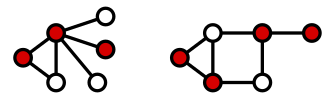
\includegraphics[width=0.5\linewidth]{images/Vertex-cover.svg.png}
    \caption{The figure shows the vertex cover of the two original graphs. The vertices in red are a set of vertex cover. Note that every edge in the graph has at least one endpoint in the vertex cover}
    \label{fig:enter-label}
\end{figure}
The dual of maximum matching problem corresponds to the minimal vertex cover in the graph. \cite{yiu2023research} While the LP solution may give fractional values, for bipartite graphs, the dual LP has an integral solution, as shown in the König's theorem.

\subsection{König's Theorem and its Application}
Kőnig’s Theorem \cite{Konig1916} asserts that in any bipartite graph, the size of the maximum matching equals the size of the minimum vertex cover. 

\begin{proof}[Kőnig's Theorem]
    In any bipartite graph \( G = (U, V, E) \), the size of the maximum matching equals the size of the minimum vertex cover. That is,
    \[
    \text{size(Maximum Matching)} = \text{size(Minimum Vertex Cover)}.
    \]
\end{proof}


\section{Integer Programming}
\label{sec:integer_programming}
\label{IP}
%Jacob COMPLETE

%\subsection{Integer Programming} \label{IP}

%Introduction
%NP-Hardness
%How to Solve
%Maximum matching via integer programming
%The Matching Polytope

\subsubsection{Introduction}\label{IPintro}

Integer programming is a discrete variant of linear programming.

\begin{definition}
    An integer program is specified by the same information as a linear program: variables, an objective function and constraints.
    A feasible solution for an integer program is a feasible solution for the corresponding linear program, its \textit{LP relaxation}, such that each variable is assigned an integer.
    An optimal solution is a feasible solution with the maximum value amongst feasible solutions.
    The computational problem \textit{integer programming} is defined as in the linear case.
\end{definition}

\begin{remark}
    In integer programming, is the variables that must be integers, not the coordinates of the linear functions involved.
\end{remark}

\begin{example}
    For $\lambda \in \R$, consider the following integer program with variables in two variables $x$ and $y$:

\begin{center}
Maximize $y$

Subject to the constraints

$0 \leq \lambda y - x \leq 0$

$y \geq 1$.

\end{center}

A feasible solution to this integer program is a witness that $\lambda$ is rational.
Hence this linear program is infeasible when $\lambda$ is irrational, while it is unbounded if $\lambda$ is rational.
Note that its LP relaxation is always irrational.
\end{example}

\begin{notation}
    If $I$ is an integer program, we write $\tilde{I}$ for its LP relaxation.
\end{notation}

\begin{example}\label{0-1}
Another variant of integer programming is 0-1 integer programming where integers are replaced with binary values.
It is a special case of integer programming obtained by adding the constraints $0 \leq x \leq 1$ for all variables $x$ to an integer program.
This is useful because binary variable assignments correspond to propositional functions and hence to subsets of the variable set.
\end{example}

\subsubsection{NP-Hardness}\label{IPisNPhard}

We saw earlier that linear programming is in the class P.
Despite its similarity to linear programming, integer programming is much harder.
In fact, we have the following:

\begin{theorem}\label{nphard}\cite{karp21}
    Integer programming is NP-hard.
\end{theorem}

\begin{proof}
In fact, we will show 0-1 integer programming as in \Cref{0-1} is NP hard by reducing SAT to it.
Let $C_{1}, \ldots, C_{m}$ be the clauses of a formula in CNF with variables $x_{1}, \ldots x_{n}$. 
Our 0-1 program will have variables $y_{1}, \ldots, y_{n}$ with objective
    
\begin{center}
Maximize $0$

Subject to the constraints

For all $0 \leq j \leq m$, $\sum_{x_{i} \in C_{j}} (-y_{i}) + \sum_{\neg x_{i} \in C_{j}} y_{i} \leq (\#\text{ of negated variables in } C_{j}) - 1$.

\end{center}

The objective function being constant ensures any feasible solution is optimal, so it suffices to show feasible solutions are the same as satisfying assignments of $\bigwedge_{j = 1}^{m}C_{j}$.
For $y_{1}, \ldots, y_{n} \in \{0, 1\}$ and $0 \leq j \leq m$, observe that $\sum_{x_{i} \in C_{j}} (-y_{i}) + \sum_{\neg x_{i} \in C_{j}} y_{i} \leq (\#\text{ of negated variables in } C_{j}) - 1$ if and only if either a $y_{i}$ in the first sum is 1 or a $y_{i}$ in the second is 0.
Equivalently, clause $C_{j}$ is satisfied under the corresponding variable assignment. The result follows.
\end{proof}

\subsubsection{How to Solve}\label{solvingIP}

In spite of \Cref{nphard}, there are known methods to make integer programming tractable in practice.
The basic idea is as follows.

Suppose given an integer program $I$.
A first approximation to an optimal solution to $I$ would be an optimal solution to its LP relaxation $\tilde{I}$.
Of course, such a solution may not exist. If this is the case, the fundamental theorem of linear programming tells us that either $\tilde{I}$ is infeasible or unbounded.
In the first case, $I$ has no optimal solution and we are done.
The latter is more troublesome, but we ignore this case since it is uncommon in applications.

Say $x$ is an optimal solution to $\tilde{I}$. If $x$ is integral, we are done.
Otherwise, there is a fractional coordinate $\floor{x_i} < x_i < \ceil {x_i}$. Any optimal solution $y$ to $I$ must have $y_{i} \leq \floor{x_i}$ or $\ceil{x_i} \leq y_i$.
Hence our problem breaks into two subproblems $I'$ and $I''$ where $I'$ is $I$ with the added constraint $y_{i} \leq \floor{x_i}$ and $I''$ is $I$ with the added constraint $\ceil{x_i} \leq y_i$.
If we can solve $I'$ and $I''$, the solutions can be pieced together as follows:

\begin{itemize}
    \item If both have optimal solutions, the one with greater objective value works (or either if they have equal objective value).
    \item If only one has an optimal solution, that solution works.
    \item If neither has an optimal solution, $I$ does not either.
\end{itemize}

Thus, we have a recursive algorithm for solving integer programming.
There are two obvious questions:

(1) Does this process terminate?
If the feasible region of $\tilde{I}$ is bounded, the answer is yes.
Indeed, if the feasible region is contained in the rectangle $[a_1, b_1] \times [a_2, b_2] \times \ldots \times [a_n, b_n]$ with $a_{i}, b_{i} \in \Z$, the feasible regions of $\tilde{I'}$ and $\tilde{I''}$ are contained in properly smaller rectangles with integer corners.

(2) Is this algorithm efficient or at least is it usually efficient?
The answer is no, in its current form.
As it is, a lot of the work the algorithm does is superfluous.
For example, suppose we have found an optimal solution $x$ to $I'$ and $x$ has objective value larger than that of the optimal solution to $\tilde{I''}$.
Then also any objective solution to $I''$ also has smaller objective value than $x$, so we can stop immediately and return $x$.
Taking this shortcut cuts the running time in half. 
By taking similarly shortcuts recursively, we can cut the time down more.

In the general context, it is useful to picture the integer programs being searched as a binary tree.
At any time, we store as a bound the largest objective value of integral solutions obtained.
For a leaf associated to an integer program $J$, we branch into two subtrees only if the solution to $\tilde{J}$ has objective value at the least the bound.
This is called the \textit{branch and bound} method and fulfills our goal of solving integer programming quickly.

In practice, integer program solvers use more sophisticated techniques for the branching step, but the general strategy is the same.

\subsubsection{Maximum Matching via Integer Programming}\label{MMviaIP}

\begin{definition}\label{I(G)}
    
Given a hypergraph $G = (V, E)$ and $v \in V$, let $\delta(v)$ denote $\{e \in E \mid v \text{ is incident to } e\}$.
We define the integer program $I(G)$ with variables indexed by $E$ as follows:
\begin{center}
Maximize $\sum_{e \in E} x_e$

Subject to the constraints

(1) For each $e \in E$, $0 \leq x_e$

(2) For each $v \in V$, $\sum_{e \in \delta(v)} x_e \leq 1$.

\end{center}
\end{definition}

\begin{lemma}\label{integerlemma}
    Feasible points for $I(G)$ correspond to matchings of $G$.
\end{lemma}

\begin{proof}
    Let $x \in \R^E$. Given \Cref{I(G)} (1), \Cref{I(G)} (2) is equivalent to ($2^{\prime}$) $x_e \leq 1$ for all $e \in E$ and ($2^{\prime \prime}$) for all $v \in V$ there is at most one $e \in \delta(v)$ such that $x_e = 1$. 
    Integrality along with \Cref{I(G)} (1) and ($2^{\prime}$) is equivalent to all the $x_e$ being binary i.e. $x \in \{0,1\}^E$.
    And $(2^{\prime \prime})$ is equivalent to $\{e \in E \mid x_e = 1\}$ being a matching.
    Thus the bijection $\{0,1\}^E \cong \mathcal{P}(E)$ restricts to a bijection between $x \in \R^E$ satisfying \Cref{I(G)} (1) and (2) to matchings of $G$.
    \end{proof}

\begin{corollary}
    Solving $I(G)$ is tantamount to finding a maximum of $G$.
\end{corollary}

\begin{proof}
    For $x \in \R^E$ satisfying \Cref{I(G)} (1) and (2), $\sum_{e \in E} x_e$ is the size of the corresponding matching as in \Cref{integerlemma}.
    So optimal solutions to $I(G)$ correspond to maximum matchings of $G$.
\end{proof}

Hence the maximum matching problem may be solved by using an integer programming algorithm on the problem $I(G)$.
As integer programming is NP-complete, one cannot expect this solution to run in polynomial time.
In fact, it is not even clear this method will find run in polynomial time when $G$ is bipartite.
To remedy this, we introduce the concept of the matching polytope.

\subsubsection{The Matching Polytope}\label{matchingpolytope}

Unlike its integral counterpart, linear programming can be solved in polynomial time, using the simplex algorithm.
This suggests that we consider the LP relaxation $L(G) = \widetilde{I(G)}$.

\begin{definition}
    The (fractional) \textit{matching polytope} of $G$, denoted $FM(G)$ is the feasible region of $L(G)$ i.e. $\{x \in \R^E \mid \text{ for all }e \in E,\text{ }0 \leq x_e \text{ and for all $v \in V,\text{ }\sum_{e \in \delta(v)} x_e \leq 1$}\}$.
    Let $IM(G)$ be the integer points of $FM(G)$ and $M(G)$ the convex hull of $IM(G)$.
\end{definition}

\Cref{integerlemma} says points of $IM(G)$ correspond to matchings of $G.$
Since $FM(G)$ is convex, $M(G) \subset FM(G)$.

\begin{theorem} \label{matching polytope} \cite{edmonds}
    For $G$ an ordinary graph, $M(G) = FM(G)$ if and only if $G$ is bipartite.
\end{theorem}

\begin{proof}

($\Rightarrow$) Suppose $M(G) = FM(G)$. We will show $G$ contains no odd cycles.
For suppose $C$ is a cycle of odd length $n$; it can be assumed $C$ is simple.
Define $y \in \R^E$ by $y_e = \frac{1}{2}$ for $e \in C$ and $y_e = 0$ otherwise. Since $C$ is simple, $y \in FM(E)$ and so $y \in M(G)$ by assumption. 
    
Now consider $\{x \in \R^E \mid \sum_{e \in C}x_e \leq \frac{n - 1}{2}\}$.
This set of convex and it is not hard to see that it contains $IM(G)$.
Thus it contains $M(G)$ and, in particular, $y$.
This contradicts $\sum_{e \in C}y_e = \frac{n}{2} > \frac{n - 1}{2}$.

($\Leftarrow$) It will suffice to prove every extreme point of $FM(G)$ is in $IM(G)$.
To do this we take $x \in FM(G) - IM(G)$ and show it is not an extreme point.
Let $e_0 \in E$ be such that $0 < x_{e_0} < 1$ and $P$ a maximal simple path or cycle extending $e_0$ such $0 < x_e < 1$ for all $e \in P$.
Set $\epsilon = \min\{x_e, 1 - x_e \mid e \in P\}$, $x'$ to be $x$ with $\epsilon$ added at even edges of $P$ and subtracted at odd edges of $P$ and $x''$ to be $x$ with $\epsilon$ subtracted at even edges of $P$ and added at odd edges of $P$.
These are well defined because $P$ is simple and has even length if it is a cycle.

Since $\epsilon \leq x_{e}$ for all $e \in P$, \Cref{I(G)} (1) holds for $x'$ and $x''$.
Let $v \in V$; we will show $\sum_{e \in \delta(v)} x'_e,$ $\sum_{e \in \delta(v)} x''_e \leq 1$.
If $v$ is not in $P$ or is in $P$ but not an endpoint, $\sum_{e \in \delta(v)} x'_e = \sum_{e \in \delta(v)} x''_e = \sum_{e \in \delta(v)} x_e \leq 1$ by construction.
If $v$ is an endpoint, the condition $\epsilon \leq 1 - x_e$ for $e$ the one edge adjacent to $v$ ensures the condition.
Since $0 < x_e < 1$ for all $e \in P$, we have $0 < \epsilon$ so $x \neq x', x''$.
But $x = \frac{1}{2} x' + \frac{1}{2} x''$, so $x$ is not an extreme point of $FM(G)$.

\end{proof}

\begin{scholium}
    If $G$ is Bipartite, $I(G)$ can be solved in polynomial time with respect to $G$.
\end{scholium}

\begin{proof}
    The proof of \Cref{matching polytope} showed every extreme point of $FM(G)$ is in $I(G)$.
    As the simplex algorithm returns an extreme point of the feasible region, its solution is automatically integral. 
\end{proof}


\section{Independent Sets} \label{sec:IndSets}
%\subsection{Independent Sets} \label{IndSets}

\begin{definition}
    Let $G$ be a graph. A subset $S$ of $G$ is called \textit{independent} if no two distinct vertices of $G$ are adjacent. The maximum independent set problem is the problem of finding an independent set of greatest size in a graph $G$.
\end{definition}

\begin{example}
    Take $G$ to be the following graph. Both the red and blue sets are independent in $G$, but only the blue set is maximum.
    
    \begin{center}
\begin{tikzpicture}[scale=1.5]

    \node[circle, draw, red] (a) at (0,1) {1};
    \node[circle, draw, blue] (b) at (1,2) {2};
    \node[circle, draw, blue] (c) at (1, 0) {3};
    \node[circle, draw, red] (d) at (2,1) {4};
    \node[circle, draw, blue] (e) at (3,1) {5};
    \node[circle, draw, red] (f) at (4,1) {6};
    \node[circle, draw, blue] (g) at (5,2) {7};
    \node[circle, draw, blue] (h) at (5,0) {8};
    \node[circle, draw, red] (k) at (6,1) {9};

    \draw[thick] (a) -- (b);
    \draw[thick] (a) -- (c);
    \draw[thick] (b) -- (d);
    \draw[thick] (c) -- (d);
    \draw[thick] (d) -- (e);
    \draw[thick] (e) -- (f);
    \draw[thick] (f) -- (g);
    \draw[thick] (f) -- (h);
    \draw[thick] (g) -- (k);
    \draw[thick] (h) -- (k);

\end{tikzpicture}
\end{center}
\end{example}

The definitions of matching and independent set are visibly similar: they differ by replacing 'vertex' with 'edge' and 'shares a vertex' with 'adjacent'. This inspires a concrete way to relate the two problems.

\begin{construction}\label{edgegraph}
    Let $H$ be a hypergraph. We define its \textit{edge graph} $E(H)$ as follows:

    The vertices of $E(H)$ are the hyperedges of $H$.

    Two distinct hyperedges $e$ and $e'$ have an edge between them if and only if $e$ and $e'$ share a vertex.
\end{construction}

Expanding the definitions, an independent set in $E(H)$ is exactly a matching for $H$.

\begin{proposition}
    The maximum matching problem for hypergraphs and the maximum independent set problem are reducible to one another. 
\end{proposition}

\begin{proof}
    By construction, an independent set in $E(H)$ is exactly matching for $H$. Thus a maximum independent set in $E(H)$ is the same as a maximum matching for $H$, showing the maximum matching problem reduces to the maximum independent set problem.
    
    For the other direction, it suffices to show every graph can be realized as $E(H)$ for some $H$. Let $G$ be a graph and enumerate its edges $e_{1}, e_{2}, \ldots, e_{m}$. Take $H$ to be a $m$-partite hypergraph with edges corresponding to the vertices of $G$ so that for each $1 \leq i \leq m$, only the two edges of $e_{i}$ share a vertex. By construction the vertices of $E(H)$ correspond to those of $G$ with an edge between them if and only if the corresponding vertices have an edge in $G$.
\end{proof}

\begin{remark}
    In fact, the maximum independent set problem is reducible to 3-dimensional max matching, since both are NP-complete. \cite{karp21}
\end{remark}


\section{Stable Marriage Problem (SMP)}
\label{sec:smp}
\section*{Introduction} 
While not a reduction problem but instead a variant of the original Maximum Matching Problem, we can use the Stable Marriage Problem to better understand the nature and time complexity of the original problem. Through the use of matching people with relationships to one another, we already have a much more intuitive example of the original problem. By increasing the number of non-overlapping sets, relationships get increasingly more complex to map, growing from P class to NP-complete by simply going from bipartite to d-partite graphs. In this case, we consider the bipartite version to be the original problem proposed by Gale and Shapley and the 3D Stable Marriage Problem variant to be the d-partite variant. It is also by using stable matchings that we can find a max-matching, unless we use a Stable Marriage variant that specifically omits this property. 

This section summarizes the problem structure and several algorithms presented in Dan Gusfield and Robert W. Irving's book "The Stable Marriage Problem." It covers foundational knowledge necessary to understand the nature and complexity of the problem. Additionally, it surveys recent papers on the topic, illustrating how the problem and its accompanying algorithms has developed since the book's release in 1989. The paper examines the Gale-Shapley algorithm \cite{galeshapley} alongside several other relevant algorithms that have emerged since then.  

We’ll break down the key structure and algorithms presented in Dan Gusfield and Robert W. Irving’s work, "The Stable Marriage Problem." The goal here is to provide a solid understanding of the problem’s core concepts, particularly how stability and preferences interact within the context of algorithmic solutions like the well-known Gale-Shapley algorithm. After laying that groundwork, we’ll dive into a survey of relevant papers that have been published after the book’s release in 1989. These papers showcase the evolution of the problem, introducing new angles and improvements to the algorithms initially discussed. This includes updates on the theoretical complexity, practical applications, and how researchers have expanded upon the stable marriage framework in various ways.

\section*{Definitions}
The following section covers the definitions from the Gusfield and Irving book that are essential when understanding the Stable Marriage Problem (SMP) and its variants. This section serves as a reference since these terms will be used frequently in this section.
\begin{itemize}
    \item \textbf{Stable Matching}: A matching is called \emph{stable} if there are no two people, one from each side of the marriage problem, who would both prefer each other over their current partners. In other words, there are no \emph{blocking pairs}. Stability ensures that no person has the incentive to deviate from the matching.
    
    \item \textbf{Preference Lists}: Each individual in the SMP has a strict ordering of the members of the opposite group, ranking them based on preference. These rankings are used to determine which matchings are stable. Preference lists are central to the algorithmic process for finding stable matchings.
    
    \item \textbf{Unacceptable Partners}: In some variations of the SMP, an individual may consider certain members of the opposite group as \emph{unacceptable}. In such cases, they would rather remain unmatched than be paired with an unacceptable partner. These unacceptable partners are omitted from the individual’s preference list or at a position in the list where the agent would receive negative utility from being matched with them.
    
    \item \textbf{Indifference}: This refers to situations where an individual does not have a strict preference between two or more potential partners. Indifference leads to \emph{ties} in preference lists, complicating the stability conditions and algorithms used to find a stable matching. In the basic SMP, preference lists are assumed to be strict, but variations of the problem allow for the indifference property.
    
    \item \textbf{Blocking Pair}: A pair of individuals form a \emph{blocking pair} if they prefer each other over their current partners in a matching. The existence of any blocking pair makes a matching unstable. Blocking pairs only exist in the bipartite graph version of the problem. Thus, stability is defined as the absence of blocking pairs.
    
    \item \textbf{Optimality}: In the SMP, \emph{optimality} refers to a solution where one side of the matching get the best possible partner they could have in any stable matching. For instance, in the \emph{man-optimal} stable matching, each man is matched with the best partner they can get, considering stability.
    
    \item \textbf{Pessimality}: The opposite of optimality. In a \emph{man-pessimal} stable matching, each man is paired with the worst partner they could have in any stable matching. The pessimal matching is still stable but represents the least favorable outcome for one side.
    
    \item \textbf{Regret}: The \emph{regret} of an individual in a stable matching is defined as the ranking of their partner in their preference list. Lower-ranked partners lead to higher regret. Minimizing regret is a goal in finding a desirable stable matching for individuals.
    
    \item \textbf{Egalitarian Costs}: The \emph{egalitarian cost} of a stable matching is the total sum of regrets of all individuals in the matching. It is used to measure the overall dissatisfaction in a stable matching. The goal of \emph{egalitarian stable matching} is to minimize the total regret across both sides of the matching problem. \cite{gusfield} 
\end{itemize}

It's important to note that preference lists and accompanying definitions are not present in the original Maximum Matching problem but they significantly enhance its applicability to real-world scenarios. Stability ensures that no matched pair would prefer an alternative arrangement, minimizing disruptions and allowing for longer-lasting solutions in applications like job assignments or roommate pairings. This stability is crucial in scenarios where frequent rearrangements are undesirable, as in hospital residency placements. These elements improve the practical applicability of the Maximum Matching problem.

\section*{Background}
\paragraph{Classical Setup: Stable Marriage Problem}
The problem was first studied by Gale and Shapley in 1962. The original setup of the Stable Marriage problem consists of two equally sized sets: one representing men and the other representing women. Each participant has a preference list, and the goal is to create a stable matching that maximizes preferences. 
\\
\begin{itemize}
    \item \textbf{Input:} Two equally $n$ sized non-overlapping sets $A$ and $B$, where each item in $A$ contains a preference list, $list = {b_1, ..., b_n }$, and where each item in $B$ contains a preference list, $list = {a_1, ..., a_n }$.
    \item \textbf{Output:} A graph $G = (V,E)$ that contains a stable matching where each agent from $A$ is matched to one agent in $B$. 
\end{itemize}

A blocking pair arises when an individual prefers another partner over their current one, and vice versa. The existence of a blocking pair indicates instability; if none exist, the matching is considered stable.
\cite{gusfield}

It is important to note that these notions of relationships established by Gale and Shapley are outdated and call for improvements, one of the main motivations for exploring the topic in this paper.

\paragraph{Optimality}
In stable marriage problems, there are several potential optimal solutions. The male-optimal stable solution ensures that each man is as well off as possible under any stable solution, while the female-optimal stable solution guarantees the best outcomes for the women. The minimum choice stable solution minimizes the sum of choice rankings for both men and women, providing a more balanced, 'unselfish' solution. These solutions may sometimes coincide, though they can differ based on individual preferences.
\cite{mcvitie}

\paragraph{Gale-Shapley Algorithm}
The Gale-Shapley algorithm, fundamental to solving the Stable Marriage Problem, has both male- and female-oriented versions. The algorithm proceeds as follows:

\begin{verbatim}
assign each agent to be free;
while some agent m is free do:
begin 
    w := first agent on m's preference list who has not yet been proposed to;
    if w is free then
        assign m and w to be engaged;
    else 
        if w prefers m to their partner m' then
            assign m and w to be engaged and m' to be free;
        else
            w rejects m {and m remains free};
end;
return the stable matching consisting of the n engaged pairs;
\end{verbatim} 

When dealing with sets of unequal sizes, we can still guarantee at least one stable matching, but we must also address unacceptable partners, or those who have no matches in a stable outcome, thus this algorithm cannot apply for the majority of these more complex variants. \cite{gusfield}

\paragraph{Gale-Shapley Algorithm Example}

\begin{center}
\begin{tabular}{||c c c||} 
 \hline
  $m_1$ & $m_2$ & $m_3$ \\ [0.5ex] 
 \hline\hline
 $w_2$ & $w_1$ & $w_3$ \\
 \hline
 $w_3$ & $w_2$ & $w_2$ \\
 \hline
 $w_1$ & $w_3$ & $w_1$ \\ [1ex] 
 \hline
\end{tabular}
\end{center}

\begin{center}
\begin{tabular}{||c c c||} 
 \hline
  $w_1$ & $w_2$ & $w_3$ \\ [0.5ex] 
 \hline\hline
 $m_2$ & $m_1$ & $m_3$ \\
 \hline
 $m_3$ & $m_2$ & $m_2$ \\
 \hline
 $m_2$ & $m_3$ & $m_1$ \\[1ex] 
 \hline
\end{tabular}
\end{center}

\begin{center}
    \textbf{Preference Lists Example}
\end{center}

\begin{center}
\begin{tikzpicture}[scale=1.5]
    % Draw nodes for men
    \node[circle, draw] (1) at (0, 1) {$m_1$};
    \node[circle, draw] (2) at (0, 0) {$m_2$};
    \node[circle, draw] (3) at (0, -1) {$m_3$};

    % Draw nodes for women
    \node[circle, draw] (4) at (1, 1) {$w_1$};
    \node[circle, draw] (5) at (1, 0) {$w_2$};
    \node[circle, draw] (6) at (1, -1) {$w_3$};

    % Draw edges representing the stable matching
    \draw[thick] (1) -- (5);
    \draw[thick] (2) -- (4);
    \draw[thick] (3) -- (6);
\end{tikzpicture}
\end{center}

\begin{center}
    \textbf{Stable Matching Example}
\end{center}

To illustrate the Gale-Shapley algorithm, we start with $m_1$ and perform the $m$-optimal Gale-Shapley algorithm, where each man proposes to their most preferred woman who hasn’t yet rejected them. This process yields the stable matching: \( \{(m_1, w_2), (m_2, w_1), (m_3, w_3)\} \), which is computed in polynomial time.

\paragraph{Runtime Complexity}
In this classical form of the problem, the worst-case complexity is $O(n^2)$, where $n$ is the number of men and also women. This arises from the necessity to check each individual's preferences and potential matches. \cite{gusfield}

\paragraph{Pre-Survey Remarks}
The Stable Marriage Problem is tied closely to concepts in computational complexity, particularly when considering extensions or variations of the problem that can grow in computational complexity. The original problem serves as an illustration of the divide between problems that can be solved efficiently and those that are computationally difficult, NP-hard or NP-complete. 

While the classic stable marriage problem with the Gale-Shapley algorithm can be solved in polynomial time, many of its variations, such as finding a stable matching under additional constraints, mentioned in latter portions regarding ties in preferences, incomplete preference lists, can grow to be NP-complete and/or NP-hard.

Another notable variant, the Stable Roommates Problem\cite{gusfield}, seeks to find a stable matching among a single group of individuals, without predefined pairings. In this scenario, stability is not guaranteed, and finding a matching can become computationally challenging, particularly with extensions that push it into NP-complete computational complexity.

These complexities illustrate how adding real-world constraints can dramatically alter the computational complexity, pushing problems into more complex realms. This highlights the importance of studying these problems as a means to produce equitable outcomes for all individuals. 

\section*{Problem Survey}
This section explores the various types of problems and algorithms presented in the book and recent literature in order to assess the progress made on these topics in subsequent research.

\paragraph{Extended Gale-Shapley Algorithm}

The \emph{Extended Gale-Shapley Algorithm}, developed by Robert Irving and Dan Gusfield, refines the classic Gale-Shapley algorithm to address the stable marriage problem while accommodating complexities such as ties in preferences and incomplete preference lists. This algorithm allows for equal rankings among choices, where an agent may rank two agents equally, thus reflecting indifference, and handles scenarios where participants may not rank all members of the opposite group. The algorithm also maintains the order of preferences and resolves ties consistently, often using secondary criteria to break ties. Furthermore, the algorithm has practical applications in various fields, including medical residency matching, school assignments, and job recruitment, enhancing its use in realistic scenarios where preferences are not always defined.

This extension helps address scenarios with unequal sets and considers preferences that include indifference or unacceptable partners, leading to a more nuanced approach to finding stable matchings. \cite{gusfield}

\paragraph{Irving Stable Roommates Algorithm}
This algorithm provides a framework for solving the Stable Roommates Problem, allowing for a stable matching among a single group without predefined pairings. It introduces additional complexity in finding and verifying stable matches.
\cite{gusfield}

This problem's importance is evident as the system is still used today and will be for the foreseeable future. While not as crucial as relationship matching or kidney exchanges, colleges continue to look for ways to maximize satisfaction among students and their roommates.

\paragraph{Hospital and Resident Problem}
An application of the Stable Marriage framework, this problem addresses the allocation of medical residents to hospitals based on mutual preferences. It extends the original problem to allow for multiple residents being mapped to  single hospital, showcasing practical implications and the need for variation of the original problem. 

Furthermore, the Gale-Shapley algorithm is crucial in medical residency matching through the National Resident Matching Program (NRMP) in the United States. By efficiently pairing medical graduates with residency programs. While not the most equitable, this system can help minimize dissatisfaction and turnover among residents and programs and also seems to enhance the overall quality of medical training.
\cite{gusfield}

\paragraph{Equitable Stable Marriage Problem}
The \emph{equitable stable marriage problem} aims to minimize the maximum regret across all participants in the matching. In this version, the goal is to find a stable matching that spreads dissatisfaction evenly, ensuring that no single participant feels disproportionately worse off than the others. The aim is to make the most dissatisfied person's outcome as favorable as possible, reducing the overall disparity in dissatisfaction among participants.

The paper from Giannakopoulos et. al\cite{equitable} introduces an approach to the Equitable Stable Marriage Problem (ESMP), which was a problem initially proposed by Gusfield and Irving. The ESMP is computationally more complex and considered NP-hard. This makes finding an optimal solution efficiently highly unlikely and calls for the use of either a heuristic or approximation algorithms. Previous approximation algorithms and heuristics, have encountered limitations, particularly in terms of non-termination or impractical runtimes when applied to large datasets. The new method focuses on minimizing the gap between men’s and women’s sum-of-rankings of their spouses while still ensuring stability.

When comparing this approach with the original SMP, several key differences emerge. The Gale-Shapley algorithm, while ensuring a stable solution, tends to favor the proposing side, resulting in biased outcomes. The ESMP, on the other hand, seeks to reduce this bias by achieving equitable matchings, minimizing the difference in rankings between the two sides. Although the ESMP is NP-hard and thus more complex than the SMP. Additionally, the original SMP focuses solely on stability, without consideration for fairness, while the ESMP aims to optimize both stability and equity, ensuring that both sides have more balanced satisfaction levels in the match. In practical terms, the original SMP is straightforward to implement and guarantees termination with a stable solution, while prior solutions for the ESMP, such as Swing, have struggled with efficiency.

The algorithm from Giannakopoulos et. al\cite{equitable} is shown below.

\paragraph{Equitable Stable Marriage Algorithm:}
This algorithm seeks to find a stable matching between two groups where no one has disproportionate dissatisfaction with their match. It works by having individuals propose and evaluate potential partners in each iteration, trying to balance the regret between participants.

\paragraph{Main Steps}

\paragraph{Proposal Evaluation}
When someone receives a proposal, they compare it to their current partner:
\begin{itemize}
    \item If the proposer is better than their current partner, they break up with their old partner and accept the new one.
    \item If the proposer is not better, they reject the proposal.
    \item If a person accepts the new proposer, they also check if they can slightly improve their future choices (adjusting their satisfaction threshold for better partners).
\end{itemize}

\paragraph{Making Proposals}
A proposer makes an offer to the next person on their list:
\begin{itemize}
    \item If their current partner is not their best option, they propose to the next person.
    \item If the proposal is accepted, they get engaged to the new partner and break up with the old one.
    \item If rejected, they move on to the next option.
\end{itemize}

\paragraph{Iterative Case}
The algorithm runs in rounds:
\begin{itemize}
    \item In each round, an agent from a group/set is chosen to make proposals, either group A or group B, depending on a mathematical rule involving sine function. The oscillating function allows for randomness when selecting proposers and not simply choosing one group/set of agents as done in the original SMP.
    \item Every person in the chosen group proposes to someone, and this continues until no one wants to change their current match.
\end{itemize}

\paragraph{Termination Case}
The algorithm stops when everyone is content with their current match, no more proposals or breakups are happening. At this point, the solution is stable and equitable. Although, the authors have noted issues with their termination cases.

\paragraph{Description}
The algorithm works by having people from two groups propose to one another, aiming to minimize the worst-case dissatisfaction for anyone. People take turns proposing, and they will keep switching partners until they find someone who makes them happy enough that they stop looking for someone better. The process continues until no one wants to switch partners anymore, resulting in a stable and fair outcome for both groups. By alternating the group that proposes in each round, the algorithm grows in complexity but also ensures fairness in the matching process. 

\paragraph{Egalitarian Stable Marriage Problem}
Similar to the previous problem, the \emph{egalitarian stable marriage problem} seeks to minimize the total sum of the participants' ranks of their assigned partners. In this formulation, each individual ranks their possible partners in order of preference, and the objective is to find a stable matching that produces the lowest possible total rank sum, thus maximizing collective satisfaction. This version of the problem emphasizes fairness at a societal level, ensuring that as many participants as possible get partners they prefer higher on their lists.

The problem is also categorized as NP-hard and has several usable heuristics and approximation algorithms. Many of the algorithms make use of rotation partially ordered sets (rotation posets). The rotation posets can be used to find all stable matching of the problem and then find the optimal solution. The rotations occur until the change becomes the desired change in egalitarian costs or decreases. This draws inspiration from the Gusfield and Irving's Minimum Egalitarian Stable Marriage Problem\cite{gusfield}.

An algorithm that solves the Egalitrian SMP usually involves rotation posets \cite{mcdermid}. The following is a high level description of an algorithm from Siyuan Wu et. al \cite{wu}.

\paragraph{Egalitarian Stable Marriage Algorithm:}

\paragraph{How the Algorithm Works}

\begin{enumerate}
    \item \textbf{Initial Stable Matching (Gale-Shapley)}: 
    \begin{itemize}
        \item The algorithm begins by finding any stable matching using a basic stable marriage algorithm (the Gale-Shapley algorithm).
        \item This provides a starting point for further refinement, but it is not necessarily the most egalitarian.
    \end{itemize}
    
    \item \textbf{Identifying Rotations}:
    \begin{itemize}
        \item Once a stable matching is found, the algorithm identifies all rotations. A rotation represents a set of men and women who could essentially "swap" partners in a way that makes at least one of them happier without violating stability.
        \item Each rotation consists of a sequence of matched pairs, where each man can improve his match by switching to another woman in the rotation.
    \end{itemize}
    
    \item \textbf{Rotation Poset Construction}:
    \begin{itemize}
        \item The rotations identified form a poset, partially ordered set. Some rotations depend on others, meaning you cannot apply one rotation until another has been performed.
        \item This structure ensures that the algorithm respects dependencies when performing rotations, preventing any conflicts in stability.
    \end{itemize}
    
    \item \textbf{Applying Rotations}:
    \begin{itemize}
        \item The algorithm traverses the rotation poset, removing rotations that reduce the total dissatisfaction. By applying a rotation, some individuals get matched with partners they prefer over their current ones.
        \item The algorithm continues applying rotations in the correct order to reduce the overall dissatisfaction incrementally.
    \end{itemize}
    
    \item \textbf{Termination}:
    \begin{itemize}
        \item The algorithm stops when no further rotations can improve the total dissatisfaction. At this point, the matching is both stable and as close to egalitarian as possible, given the constraints of stability.
    \end{itemize}
\end{enumerate}

\paragraph{Simplified Example}

\textbf{Initial Gale-Shapley Matching}: Let’s say a set of men and women are paired based on the male optimal Gale-Shapley algorithm. This produces a stable matching but not necessarily the most balanced in terms of satisfaction.

\textbf{Identifying a Rotation}: The algorithm detects a set of men and women who can improve their partners by rotating. For instance, man A prefers woman X, currently paired with man B, and man B prefers woman Y, currently paired with man C. The rotation allows them to switch partners without destabilizing the matching.

\textbf{Rotation Poset}: If man A’s improvement depends on another rotation involving man D and woman Z, the algorithm must first resolve that rotation before allowing A’s rotation to proceed. 

\paragraph{Summary of the Algorithm}

\begin{enumerate}
    \item Find a stable matching using the Gale-Shapley algorithm.
    \item Identify all possible rotations, which are sequences of pair swaps that can improve dissatisfaction without introducing instability.
    \item Construct a rotation poset to manage the dependencies between different rotations.
    \item Apply rotations in the correct order to iteratively reduce total dissatisfaction.
    \item Stop when no more rotations can be applied, resulting in an egalitarian stable matching.
\end{enumerate}

\paragraph{Sex-Equal Stable Marriage Problem}
The \emph{sex equal stable marriage problem} focuses on achieving a balanced outcome for both groups. It aims to minimize the difference in average satisfaction between the two groups. In other words, the goal is to find a stable matching where the average ranks of assigned partners are as equal as possible between the two groups of agents. This problem ensures that neither group, on average, ends up significantly better off than the other. 

Similar to the Egalitarian Stable Marriage Problem, it can also be done using rotation posets, as done by Kazuo et. al\cite{equalstable}.

\paragraph{Rotation Poset Algorithm for the Sex Equal Stable Marriage Problem: }

The algorithm seeks to find a sex-equal stable matching by minimizing the dissatisfaction between participants from two groups while maintaining stability. The steps of the algorithm are as follows:

\begin{enumerate}
    \item \textbf{Rotation Poset Construction:} \\
    The algorithm constructs a rotation poset, which captures the dependencies between different rotations, sets of pair swaps that can improve dissatisfaction. The poset ensures that rotations are applied in a valid order, preserving stability.

    \item \textbf{Initialize Best Matching:} \\
    The algorithm initializes a variable $M_b$ (M-best) to store the best matching found during the process.
    
    \item \textbf{Partition Rotations:} \\
    Rotations are divided into two sets:
    \begin{itemize}
        \item \( R_L \): Rotations with dissatisfaction greater than a threshold \( \delta \) (predefined threshold of dissatisfaction, depends on strictness desired).
        \item \( R_S \): Rotations with dissatisfaction less than or equal to \( \delta \).
    \end{itemize}
    
    \item \textbf{Iterate Over Subsets of \( R_L \):} \\
    For each subset \( R \) of rotations in \( R_L \), the algorithm computes an \emph{egalitarian matching} that minimizes dissatisfaction.

    \item \textbf{Apply Rotations in Order:} \\
    The algorithm applies or removes rotations based on the order in the poset, ensuring that dissatisfaction stays within bounds and stability is maintained.

    \item \textbf{Update Best Matching:} \\
    If a better matching is found, $M_b$ is updated.
    
    \item \textbf{Termination:} \\
    The algorithm terminates by outputting $M_b$ if a valid matching is found, or "None" if no such matching exists.
\end{enumerate}

\paragraph{Man-Exchange Problem}

\paragraph{Background}
The \emph{Man-Exchange problem} is a variant of the stable marriage problem where multiple partners can be matched, and exchanges between them occur. The goal is to create a stable matching where no pair prefers each other over their current partners. This problem extends the traditional stable marriage problem by introducing more flexibility in partner preferences and matching, which leads to more complex stability conditions. \cite{survey}

\paragraph{Time Complexity}
The time complexity of solving the Man-Exchange problem depends on the specific approach taken. For a Gale-Shapley-inspired solution, the algorithm runs in \(\mathcal{O}(n^2)\), where \(n\) is the number of agents. However, the complexity can increase if additional constraints or exchanges are introduced.

\paragraph{Possible Algorithms}
\begin{itemize}
    \item \textbf{Gale-Shapley Algorithm (adapted)}: This is an adaptation of the classical Gale-Shapley algorithm for stable marriages, extended to allow multiple partners and exchanges between them. The algorithm iteratively proposes matches and eliminates unstable pairs. \cite{gusfield}
\end{itemize}

\paragraph{Many-to-Many Matching Problem}

\paragraph{Background}
The \emph{Many-to-Many Matching problem} generalizes the stable marriage problem to allow agents on both sides to be matched to multiple counterparts. This situation often arises in real-world markets, such as job matching where applicants can be matched to multiple companies, or school admissions where students can apply to multiple schools. Each agent has preferences over the potential matches, and the goal is to find a stable matching. \cite{survey}

\paragraph{Time Complexity}
An extension of the Gale-Shapley algorithm for many-to-many matchings has a time complexity of \(\mathcal{O}(n^2 \cdot k)\), where \(n\) is the number of agents and \(k\) represents the maximum number of potential matches per agent. \cite{survey}

\paragraph{Possible Algorithms}
\begin{itemize}
    \item \textbf{Extended Gale-Shapley Algorithm}: This algorithm extends the classic deferred acceptance approach to handle many-to-many matchings, ensuring that the resulting matching is stable. \cite{gusfield}
\end{itemize}

\paragraph{Student Project Allocation Problem (SPAP)}

\paragraph{Background}
The \emph{Student Project Allocation Problem} (SPAP) involves matching students to projects based on mutual preferences. Students have ranked preferences for projects, and projects may also have preferences for students (if advisors are involved). The aim is to find a stable matching where no student-project pair prefers each other over their current assignment. \cite{survey}

\paragraph{Time Complexity}
The time complexity of the SPAP depends on the constraints and preferences involved. In its simplest form, where the problem is a straightforward matching, the complexity is \(\mathcal{O}(n^2)\). However, the problem can become NP-hard when additional constraints, such as capacities or weights, are considered. \cite{survey}

\paragraph{Possible Algorithms}
\begin{itemize}
    \item \textbf{Gale-Shapley-based Matching}: A variant of the stable matching algorithm, adjusted to handle student-project allocations while maintaining stability in the assignments. \cite{gusfield}
\end{itemize} 

\paragraph{3D Stable Matching}

\paragraph{3D Stable Matching Keywords}
Below are essential keywords along with their definitions that are needed to understand the problem. \cite{3dstable}
\begin{itemize} 
\item \textbf{cyclical preferences:} In a 3D stable matching scenario, three types of agents each have ranked preferences over the other two types, forming cycles in the preference relationships. Each agent’s preferences are defined in relation to pairs of agents from the other two types, creating a cyclical preference structure, rather than a linear one, which complicates the matching process.
\item \textbf{blocking triple:} A set of three agents, one from each group, who prefer to be matched with each other over their current assignments. This concept is analogous to a \emph{blocking pair} in traditional two-sided matching, where an unmatched pair would both be better off if they were matched. In the 3D case, a blocking triple indicates instability, as it implies that at least three agents are dissatisfied with their current matching.

\item \textbf{strongly blocking triple:} A specific type of blocking triple where each agent in the triple strictly prefers to match with the other two members of the triple over their current assignments. This strict preference implies that if the matching were altered to include this triple, all three would be better off, signaling strong instability in the current matching.

\item \textbf{weakly blocking triple:} A blocking triple where at least one agent in the triple has an equal preference (indifference) between their current assignment and the proposed new match. In other words, one or more agents do not strictly prefer the new match but would still find it at least as favorable as their current assignment, making the matching weakly unstable.

\item \textbf{strongly stable matching:} A matching is considered strongly stable if no strongly blocking triples exist. In this case, there is no set of three agents who would all strictly prefer to be matched with each other over their current matches, thus ensuring a stronger form of stability in the matching.

\item \textbf{weakly stable matching:} A matching is weakly stable if there are no blocking triples of any kind—either strongly or weakly blocking. In a weakly stable matching, no trio of agents would prefer (or even be indifferent to) forming a different matching arrangement, leading to a minimal form of stability.

\end{itemize}

\paragraph{Background}
The \emph{3D stable matching problem} generalizes the two-sided matching problem to involve three distinct sets of agents. For instance, in a research collaboration scenario, students, projects, and advisors may all have preferences over each other. The objective is to find a stable matching among all three groups, which poses significant computational challenges. \cite{survey} \cite{3dstable}

\subsubsection*{3D Stable Matching Example}

This example shows preferences for each element in three groups \( A = \{a_1, a_2, a_3\} \), \( B = \{b_1, b_2, b_3\} \), and \( C = \{c_1, c_2, c_3\} \), demonstrating a cycle where each participant has preferences over pairs in the other two groups. Each table displays preferences in columns and rows, where each row shows the rank order of preferences.

\paragraph{Preferences of Set \( A \):}
\[
\begin{array}{|c|c|c|}
\hline
a_1 & a_2 & a_3 \\ \hline
b_2 \; c_3 & b_1 \; c_1 & b_3 \; c_2 \\ \hline
b_3 \; c_1 & b_2 \; c_3 & b_2 \; c_1 \\ \hline
b_1 \; c_2 & b_3 \; c_2 & b_1 \; c_3 \\ \hline
\end{array}
\]

\paragraph{Preferences of Set \( B \):}
\[
\begin{array}{|c|c|c|}
\hline
b_1 & b_2 & b_3 \\ \hline
c_2 \; a_1 & c_1 \; a_2 & c_3 \; a_3 \\ \hline
c_3 \; a_2 & c_2 \; a_3 & c_2 \; a_1 \\ \hline
c_2 \; a_3 & c_3 \; a_1 & c_1 \; a_2 \\ \hline
\end{array}
\]

\paragraph{Preferences of Set \( C \):}
\[
\begin{array}{|c|c|c|}
\hline
c_1 & c_2 & c_3 \\ \hline
a_2 \; b_1 & a_1 \; b_2 & a_3 \; b_3 \\ \hline
a_3 \; b_2 & a_2 \; b_3 & a_2 \; b_1 \\ \hline
a_2 \; b_3 & a_3 \; b_1 & a_1 \; b_2 \\ \hline
\end{array}
\]

\begin{center}
\begin{tikzpicture}[scale=1.5]

    \node[circle, draw] (1) at (0, 1) {$a_1$};
    \node[circle, draw] (2) at (0, 0) {$a_2$};
    \node[circle, draw] (3) at (0, -1) {$a_3$};

    \node[circle, draw] (4) at (1, 1) {$b_1$};
    \node[circle, draw] (5) at (1, 0) {$b_2$};
    \node[circle, draw] (6) at (1, -1) {$b_3$};

    \node[circle, draw] (7) at (2, 1) {$c_1$};
    \node[circle, draw] (8) at (2, 0) {$c_2$};
    \node[circle, draw] (9) at (2, -1) {$c_3$};

    \draw[thick] (1) -- (5); % $a_1 - b_2$
    \draw[thick] (2) -- (4); % $a_2 - b_1$
    \draw[thick] (3) -- (6); % $a_3 - b_3$

    \draw[thick] (4) -- (7); % $b_1 - c_1$
    \draw[thick] (5) -- (8); % $b_2 - c_2$
    \draw[thick] (6) -- (9); % $b_3 - c_3$
\end{tikzpicture}
\end{center}


\begin{center}
    3D Stable Matching Example
\end{center}

In the context of a 3D stable matching problem, each element in group \( A \) seeks a stable match with an element from group \( B \) and one from group \( C \). We start with the first iteration by examining the preferences of \( a_1 \). According to \( a_1 \)’s preference list, their top choice is the pair \( (b_2, c_3) \). To check compatibility, we look at \( b_2 \)'s preferences, which list \( (c_3, a_1) \) as an acceptable match, as a lower choice. Similarly, \( c_3 \) ranks \( (a_1, b_2) \) as their third choice, making the match mutually acceptable. This results in an initial match of \( (a_1, b_2, c_3) \). Using this approach for each individual’s top preferences, we complete the first round of matching with the triples \( (a_1, b_2, c_3) \), \( (a_2, b_1, c_1) \), and \( (a_3, b_3, c_2) \), which forms an initial stable matching configuration across groups.

\paragraph{Time Complexity}
The 3D stable matching problem is known to be NP-complete, making it computationally intractable for large inputs. Due to the involvement of three sets of agents, the search space becomes exponentially large, complicating the problem even further. \cite{survey}

\paragraph{Possible Algorithms}
\begin{itemize}
    \item \textbf{Approximation Algorithms}: Due to the NP-completeness of the problem, approximation algorithms are often used in practice to find near-optimal stable matchings in a more computationally feasible manner. \cite{gusfield}
    \item \textbf{Heuristic Algorithms}: Similarly, due to the NP-completeness of the problem, heuristic algorithms are used to find near-optimal stable matchings for 3D graphs. 
    \cite{3dstable}

    As it currently stands, there is no efficient algorithms for 3D Stable Matchings and thus requires further research.
\end{itemize}

\paragraph{One-Sided Preference Lists}

\paragraph{Background}
In the \emph{One-Sided Preference Lists problem}, only one side of the market has preferences, while the other side does not. This scenario can arise in markets where one set of participants, such as students, has preferences over options that do not rank them in return. The goal is to find a matching that is "popular," meaning no other matching would be preferred by a majority of the participants. \cite{survey}

\paragraph{Time Complexity}
The complexity of solving the One-Sided Preference Lists problem varies depending on the approach used, but it is often polynomial-time solvable for basic versions of the problem. \cite{gusfield}

\paragraph{Summary of Time Complexities}
\begin{table}[h!]
\centering
\begin{tabular}{|p{7cm}|c|}
\hline
\textbf{Problem} & \textbf{Time Complexity} \\
\hline
Stable Marriage Problem & \(\mathcal{O}(n^2)\) \\
Man-Exchange Problem & \(\mathcal{O}(n^2)\) \\
Many-to-Many Matching Problem & \(\mathcal{O}(n^2 \cdot k)\) \\
3D Stable Matching & NP-complete \\
One-Sided Preference Lists & \(\mathcal{O}(n^2)\) \\
Egalitarian Stable Marriage & NP-hard \\
Equitable Stable Marriage & NP-hard \\
Sex-Equal Stable Marriage & NP-hard \\
Stable Marriage Problem with Incomplete Preference Lists and Ties & NP-hard \\
\hline
\end{tabular}
\caption{Summary of Time Complexities for Matching Problems}
\end{table}

As stated earlier, we can see there is a lot of difference in complexity when comparing the original problem with its variants, highlighting that subtle changes and slightly different real-world applications greatly affect the runtime.

\section*{Real-World Application of Stable Marriage Problems}
While evidently important to the theoretical field of computer science and matching problems. It is also important to see how these algorithms are being used in contemporary society. Not only is it important to design these algorithms for equitable outcomes for all people but also to criticize when it is not being used as such. Thus, we will explore several applications in this section.

\paragraph{Modern Use of Gale-Shapley Algorithm} As stated in the paper "Testing How Dating Apps Recommend a Potential Matches for User", Soemardi et al. highlight how Tinder uses both the Gale-Shapley algorithm combined with the Elo Rating System introduced by Arpand Elo for the World Chess Federation. This has proved to be problematic as studies have shown that that the app, along with Bumble, lead to increased anxiety and problematic patterns of online dating use. \cite{calvin}

In his paper, "Are Tinder and Dating Apps Changing Dating and Mating in the USA?", Michael Rosenfield highlights how the increasing reliance on these apps that use the Gale-Shapley algorithm have become increasingly problematic via the larger problem of the effect of the Internet on social interaction. Despite the intention of both the algorithm and the dating apps to be create long lasting relationships for individuals, the overwhelming amount of data reveals that it leads to "hookups" and short-term relationships. It also seems to allow people to cycle through many different partners in a shorter period of time as they assume they can improve their compatibility with a partner despite not always being the case. \cite{Rosenfeld2018}

Outside of dating apps, the Gale-Shapley algorithm has been used in optimizing power allocation of 5G networks as seen in a paper "Optimizing 5G Power Allocation Communication: A Gale-Shapley Algorithm Approach" by Alruwaili et al. The algorithm increased total network capacity and also had good power amplitude relative to the other algorithms. While the algorithm increases overhead compared to simpler, previous algorithms, it could help future resource allocation and allow for more robust data transmission. \cite{10443942}

\section*{Conclusion}
In this section, we have explored the stable marriage problem and some if its variants. The use of these problems emphasize the importance of ensuring equitable outcomes for all people. For more information on these types of problems, readers may refer to the references, I recommend starting with the textbook, \emph{The Stable Marriage Problem - Structure and Algorithms} by Dan Gusfield and Robert W. Irving.

%\printbibliography{}
\nocite{mcvitie}
\nocite{popmatch}
\nocite{RONN1990285}
\nocite{wiki}


\section{Pairwise Kidney Exchange}
\label{sec:kidney_exchange}

\chapter{Testing and Evaluation}
    \section{Testing Philosophy}
    % Author @ Sam Appleton, IN_PROGRESS, REVIEWER @ Jeremy Perez, Due Date 11/11
\subsection{Testing and Evaluation Philosophy}
We have two goals for our testing suite: determining accuracy, and evaluating
efficiency. We want our implementation of Maximum Matching solvers to be as 
accurate and efficient as possible. In terms of accuracy, we need a wide 
variety of graphs with known maximum matchings. This allows us to check each
result from a solver against the known maximum matching. These suites of tests
let us be confident in the accuracy of our solvers, as more tests with different
criteria increase our confidence in each solver. For bipartite solvers, we use 
a basic testing suite of approximately 50 different graph instances. Each instance 
has randomly assigned edges, meaning that edge cases are more likely to occur.

These suites of tests also let us test for efficiency. We use our benchmarking 
tools in Section \ref{BenchmarkingSummary} to compare wall-clock time of our suite
of solvers in Section \ref{SolverSummary}. However, a single suite of tests does 
not give us much information about the advantages of certain algorithms. We reason
that some algorithms may excel on different types of graphs, such as dense graphs, 
spare graphs, or near perfect graphs. We create several suites of tests to address
each of these types of graphs. After running each suite with each solver, we can 
make reasonable conclusions about the strengths of each algorithm and our 
implementation of it.
    \section{Verification of Test Solutions}
        % Author @ Sam Appleton, IN_PROGRESS, Reviewer @ Jeremy Perez, Due Date 11/11
\subsection{Strategic Random d-partite Test Generation}
Creating random d-partite graphs with known maximum matching is not trivial work. 
Making a random graph and then running a solver on it is unoptimal, as it requires 
a known, correct solver. Additionally, it takes a non-negligible amount of time to
run on each generated test as $n$ increases.

The difficulty of generating test graphs is that edges have to be chosen strategically 
so that any generated graph has a known maximum matching. Randomness is still a desired 
aspect of test generation so that the testing suite is diverse, but a maximum matching
must still be derived from the created graph. 

An observation on maximum matchings is exploited to create random test graphs 
more efficiently: 
\newtheorem{observation}{Observation}
\begin{observation}
A maximum matching can only ever be as large as the number of vertices
visited in the dimension with the least amount of vertices used by all the hyperedges in 
the graph. A vertex $v$ in a dimension $d$ is defined as `visited' iff $\exists$ a hyperedge $e$
such that $e[d] = v$.
\end{observation}

\begin{figure}[t!]
    \centering
    \begin{minipage}{0.45\textwidth}
        \centering
        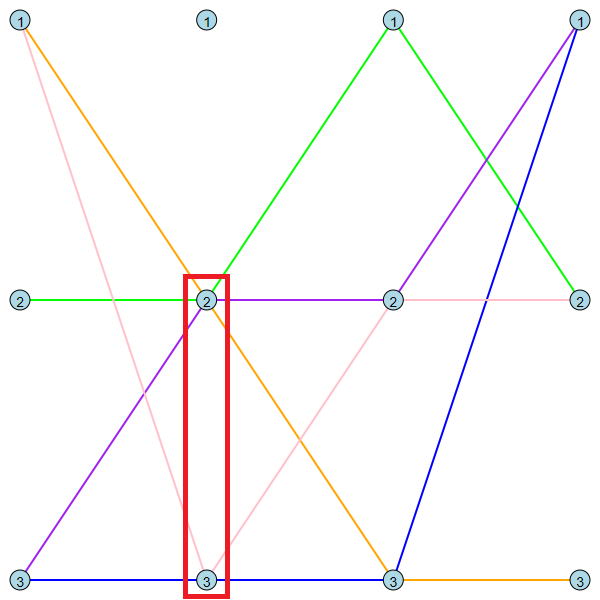
\includegraphics[width=\textwidth]{images/basic.png}
        \caption{An example of the dimension with the least visited vertices. Note that 
        every dimension except the second has an edge that goes through all three vertices.}
        \label{fig:image1}
    \end{minipage}
    \hfill
\end{figure}

This observation derives itself by considering that all hyperedges must pass
through exactly one vertex in each dimension. That means that in any of the dimensions
with the smallest number of visited vertices, at most one edge can be considered for a
maximum matching in vertex. Thus the maximum matching cannot be greater than the
number of vertices in this dimension. 

We exploit this observation to generate a graph with a known matching. To create a 
graph consisting of $d$ dimensions with $n$ vertices, $m$ hyperedges, and a maximum
matching of size $M$, consider the following algorithm:

\begin{algorithmic}
\STATE Create a $d$-partite graph $G$ with dimensions $1, 2, ..., d$ which contain vertices $1, 2, ..., n$.
\FOR{$i$ in $M$}
    \STATE Add a random hyperedge to $G$ such that the hyperedge conflicts on no dimension with any other hyperedge in $G$.
\ENDFOR
\STATE Randomly select an integer $r$ such that $1 \leq r \leq n$. 
\STATE Store the vertex in each hyperedge at index $r$ in list $included$
\FOR{$j$ in $(M - m)$}
    \STATE Add a random hyperedge $e$ such that each of the following is true:
    \begin{itemize}
        \item $e$ is not already a hyperedge in $G$, and
        \item $e[r]$ must be equal to a vertex from $included$.
    \end{itemize}
\ENDFOR
\RETURN $G$
\end{algorithmic}

This algorithm creates a graph with a known dimension with the least visited 
vertices, that being at dimension $r$. Normally this observation only yields an upper-limit 
on a maximum matching as it is not guaranteed that the maximum matching 
necessarily contains an edge for each vertex in the dimension with the least visited 
vertices. However, this algorithm guarantees that a maximum matching does visit 
each vertex, as the edges in the first for loop are guaranteed to be represented in this 
dimension. 

\begin{figure}[t!]
    \centering
    \begin{minipage}{0.95\textwidth}
        \centering
        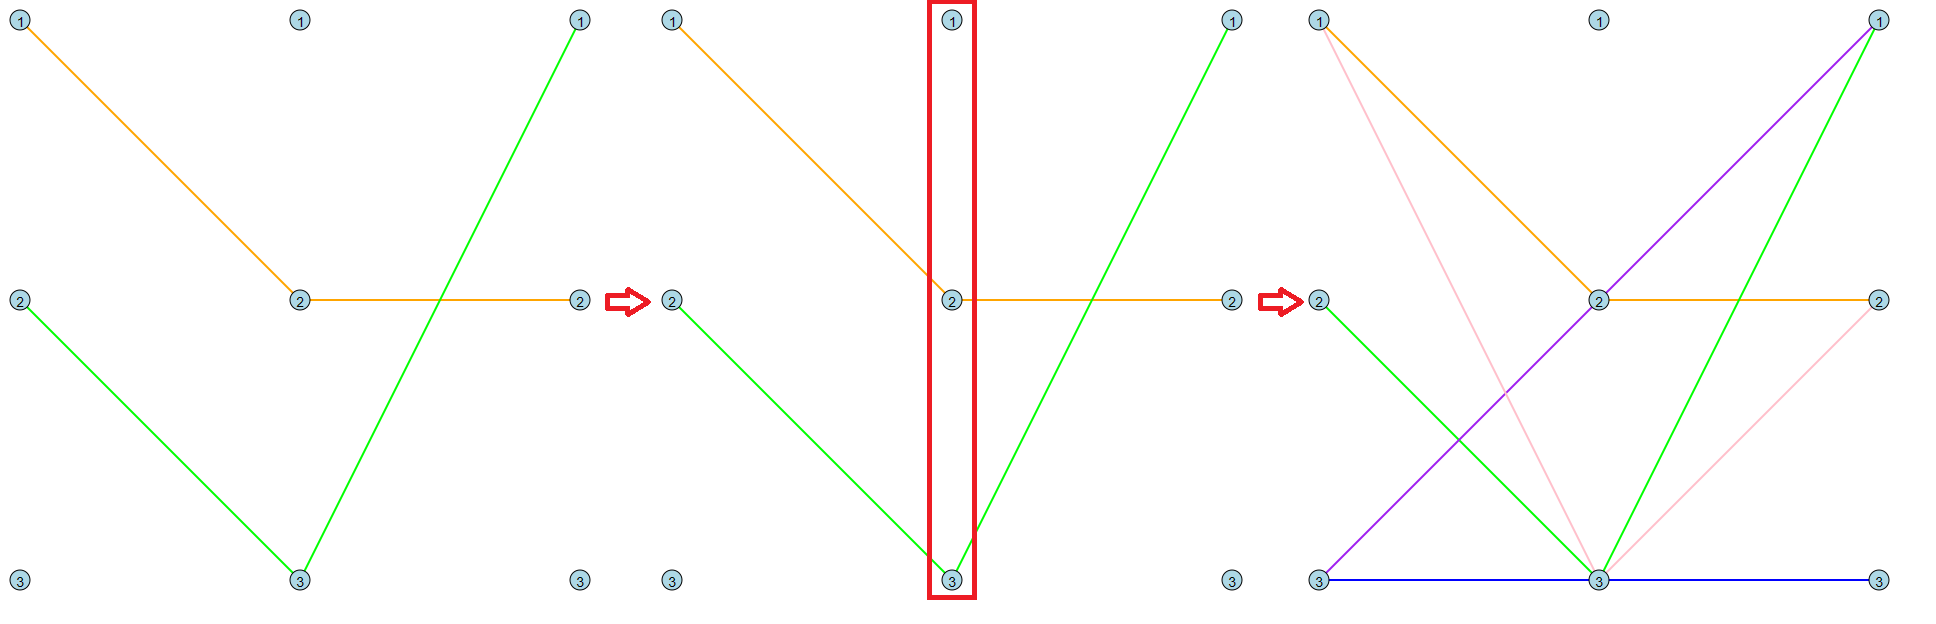
\includegraphics[width=\textwidth]{images/exclude.png}
        \caption{An example of the Dimension Restriction algorithm. In this example, a graph begins with 2 hyper edges on it. $r$ is randomly chosen to be $2$. Then more edges are added that conflict on $2$ or $3$.}
        \label{fig:image1}
    \end{minipage}
    \hfill
\end{figure}

This strategy is not without flaw. Consider a naive algorithm that determines the dimension 
with the least visited vertices and simply returns the number of visited vertices as the
 size of a maximum matching. The tests generated by this algorithm guarantee
 such an algorithm always finds the correct size of the maximum matching, and 
thus is deemed accurate despite not being so. 

A more sophisticated algorithm could be created to solve this weakness. Such an 
algorithm chooses to add hyperedges such that dimension $r$ would not necessarily 
be the dimension with the least visited vertices. To do so, this strategically adds an edge
such that it does not increase the maximum matching, 
but also visits a vertex that no other edge visits. This is done by ensuring the
added edge conflicts with some edge in the known matching on every dimension other than 
$r$, but more research can is required in this regard.
        \subsection{Automating the verification process}
        % Author @ Kurtik Appadoo, IN-PROGRESS, Reviewer @ Janak Subedi, Due Date 11/11
\subsection{Automating Test Generation}
Automating test generation offers significant advantages and presents notable challenges that must be managed to ensure reliable outcomes. Automated test generation can greatly reduce the manual time and effort required to create comprehensive test suites. By automating this process, developers can test a wide range of input scenarios, resulting in more robust and reliable software. This is especially beneficial for large-scale projects, where maintaining extensive test coverage manually is time-consuming and prone to error. Automated tests can be run consistently and repeatedly, enabling early and frequent detection of issues, thus maintaining the integrity of the codebase over time.

However, challenges arise when automating test generation for complex problem domains, such as NP-Complete problems. Generating test cases for d-partite graphs with known solutions is particularly difficult due to their computational intensity. Solving these problems often requires exhaustive search algorithms that check all possible combinations, which is resource-intensive and not easily automated without substantial computational power. The processing time and resources needed for generating and verifying such test cases make automation demanding.

Verification introduces additional complexity. Automating the verification process requires a reliable, efficient algorithm to confirm the correctness of solutions. This raises an important question: how can we ensure that the verification algorithm is accurate? This can create a cycle where the verification algorithm itself needs testing. To address this, verification is typically performed using well-established, peer-reviewed algorithms. Alternatively, a backtracking algorithm can be employed, as it guarantees correctness by exploring all possible solutions to confirm the maximum matching.

Another challenge in automated test generation is the potential bias in algorithmically generated test cases. While these instances may appear random, they are produced by human-written algorithms, which can introduce unintended patterns. This lack of complete randomness can affect the thoroughness and effectiveness of tests. For example, when generating d-partite graphs for perfect matching, it was noted that while hyperedges were generated randomly, the initial perfect matching structure often followed a pattern. This predictability posed a risk: solvers optimized to recognize such patterns might show misleading results in terms of speed and accuracy.

Addressing these issues requires introducing more randomness and variability into the generation process to create diverse test suites. Until true randomness is achieved, specialized solvers, particularly those using backtracking algorithms that exploit specific structures, may yield results that do not reflect their performance in general cases. Continuous refinement of automated test generation tools is needed to ensure they remain unbiased and representative.
    \section{Test Generation}
        \subsection{Testing File format}
        % Author @ Kurtik Appadoo, IN-PROGRESS, Reviewer @ Janak Subedi, Due Date 11/11
\subsection{Test Format}
All test files are structured using the mmi format, which is designed for representing graphs in a straightforward and consistent manner. The structure of the mmi format is detailed as follows:

\begin{itemize}
    \item The first line specifies the number of vertices in the graph, denoted as n.
    \item The second line indicates the number of partitions in the graph, referred to as d. A partition in this context is a set of vertices that only connect to vertices in other sets, not within the same set.
    \item The third line states the total number of edges or hyperedges in the graph, denoted as m. A hyperedge is a generalized edge that can connect more than two vertices, accommodating complex relationships in multi-dimensional graphs.
    \item The following m lines each represent a hyperedge in the graph, with each line containing d integers separated by spaces. These integers indicate the vertices connected by the hyperedge, ensuring connections between different partitions.
    \item The final line specifies the maximum matching in the graph, representing the maximum set of non-overlapping hyperedges where each vertex is included only once.
\end{itemize}

The mmi format is both simple and readable, making it highly suitable for generating large quantities of test cases efficiently while adhering to a standardized format. It is important to note that duplicate edges or hyperedges are not supported in this format, ensuring the uniqueness of connections within the graph.

\subsubsection{Storage and Naming Convention}
All mmi files are stored in their respective d directories within the test folder, organized by the number of partitions. Each file follows a strict naming convention to maintain clarity and consistency across the test suite:

\begin{verbatim}
    d{d}v{n}.mmi
\end{verbatim}

In this convention, d represents the number of partitions, and n indicates the number of vertices in each partition. This naming system allows for easy identification of the file contents without needing to open the file, promoting a standardized approach to organizing test cases.

\paragraph{Example}
\begin{figure}[h!]
    \centering
    \begin{minipage}{0.45\textwidth}
        \centering
        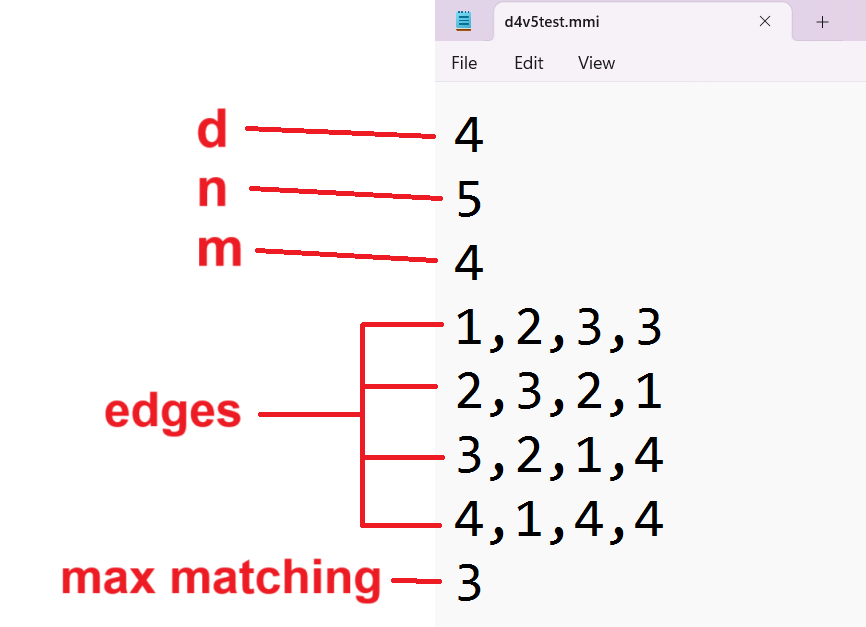
\includegraphics[width=\textwidth]{images/MMB_Solvers_Testing.png}
        \caption{An example of a test file in the mmi format.}
        \label{fig:image1}
    \end{minipage}
    \hfill
    \begin{minipage}{0.45\textwidth}
        \centering
        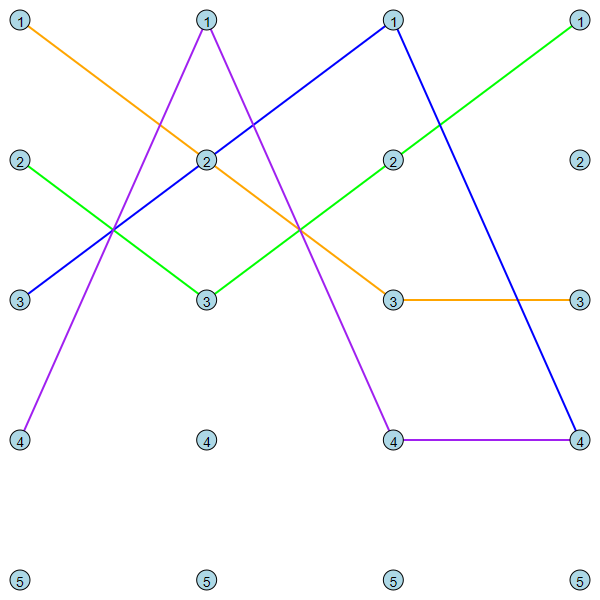
\includegraphics[width=\textwidth]{images/MMB_Solvers_Test.png}
        \caption{A visualization of the corresponding graph from Figure \ref{fig:image1}. The graph has 4 partitions, 5 vertices, and 4 hyperedges, with a maximum matching of 3 as indicated in the final line of the mmi file.}
        \label{fig:image2}
    \end{minipage}
\end{figure}

This format and naming convention provide a systematic and clear method for storing and referencing test cases, supporting efficient test generation and verification for maximum matching solvers in complex, multi-dimensional graph structures.
        \subsection{Random Test Generation}
        % Author @ Kurtik Appadoo, IN-PROGRESS, Reviewer @ Janak Subedi, Due Date 11/11
\subsubsection{Random Bipartite Graph Testing Suite}
Automating the generation of random bipartite graphs with a known maximum matching involves two main steps: generating the graph and solving it to verify the maximum matching. 

\paragraph{Challenge of Solver Validation}
Determining whether the algorithm used for solving the graph is correct can be challenging. This is because if the verification algorithm itself has flaws, it may lead to false results. To address this, we rely on algorithms that have been well-established and peer-reviewed. Additionally, backtracking algorithms, which explore all possible configurations, are often employed as they ensure correctness by checking every potential solution.

\paragraph{Approach to Generating Test Cases}
For bipartite graphs, the test generation process is simpler compared to d-partite graphs. We create two partitions, each containing n vertices, and add random edges connecting vertices from one partition to another. A random number m is generated to represent the number of edges, after which random edges are added by selecting vertices from each partition. The Graph Abstract Data Type (ADT) implementation handles duplicate edge prevention, ensuring that no repeated edges are introduced.

\paragraph{Solver Used for Verification}
To find the maximum matching in the randomly generated bipartite graphs, we used the maximum matching module from NetworkX, which is based on the well-known Hopcroft-Karp algorithm. This algorithm efficiently finds the maximum matching in bipartite graphs and is widely tested and reliable. It runs in $O(\sqrt{V}E)$ time, making it suitable for use in various applications and for verifying the test cases generated.

\subsubsection{Random D-Partite Graph Testing Suite}
Generating random graphs with a known maximum matching for d-partite graphs is more complex than for bipartite graphs due to several factors:

\begin{itemize}
    \item \textbf{Hyperedges instead of single edges}: In d-partite graphs, we work with hyperedges, which connect multiple vertices across partitions. This requires ensuring that no hyperedge or single edge duplicates exist, necessitating a data structure to track edges and prevent duplication.
    \item \textbf{Absence of polynomial-time algorithms}: Solving the maximum matching problem in d-partite graphs is NP-Hard. No known polynomial-time algorithms exist for this problem, making the task of generating test cases and verifying solutions more challenging.
\end{itemize}

\paragraph{Approach to Generating Random D-Partite Test Cases}
To generate d-partite test cases, we create a random graph with d partitions, each containing n vertices, and add hyperedges. Each hyperedge must be validated to avoid duplicate single edges or hyperedges. This validation is managed using a data structure that records all edges added to the graph. Although this introduces additional computational overhead due to search operations for every new edge, it ensures the generated test cases maintain their validity.

\paragraph{Solver Used for Verification}
Once the graph is generated, we need to solve it using a trusted solver. For d-partite graphs, where no polynomial-time algorithms exist, we initially used a brute-force algorithm. This algorithm, employing backtracking, guarantees the correctness of the maximum matching by checking all possible solutions.

\paragraph{Switch to Integer Programming Solver}
While the brute-force method ensures correctness, it is inefficient for larger graphs. To enhance the test generation process, we transitioned to an Integer Programming (IP) solver for solving d-partite graphs. This approach offered faster runtimes, enabling us to solve larger graphs within reasonable timeframes. The use of the IP solver allowed us to generate more extensive test cases and test additional solvers efficiently.

However, a limitation persists: if the IP solver and the solvers being tested share the same flaw, it may go undetected. This is an inherent limitation of the testing process and must be considered when interpreting the results of solver evaluations.
        \subsection{Test generation for pre-determined solutions}
        % Author @ Kurtik Appadoo, IN-PROGRESS, Reviewer @ Janak Subedi, Due Date 11/11

\subsection{Perfect Matching in d-Partite Graphs}
Generating random d-partite graphs is a complex task, particularly for larger and more intricate graphs. This complexity introduces potential uncertainty regarding whether all solvers, including those using integer programming, share the same bug. To address this challenge, we opted to create perfect matching d-partite graphs to ensure the accuracy of the known maximum matching by constructing graphs where the maximum matching is guaranteed.

A perfect matching in a graph is defined as a matching in which every vertex is connected by an edge, and no vertex is left unmatched. In the context of d-partite graphs, a perfect matching means that every partition in the graph has a set of edges connecting each vertex in one partition to a unique vertex in another partition. This ensures that the maximum matching is limited by the number of vertices in the smallest partition, as no matching can surpass this number.

\subsubsection{Terminology Clarification}
\begin{itemize}
    \item Matching: A set of edges where no two edges share a vertex, meaning each vertex is connected at most once.
    \item Perfect Matching: A matching that covers all vertices, so each vertex in the graph is included exactly once.
    \item d-Partite Graph: A type of graph where vertices are divided into d distinct sets, and edges can only connect vertices from different sets.
    \item Hyperedge: An edge that connects more than two vertices simultaneously, used to represent complex multi-way relationships.
\end{itemize}

\subsubsection{Generating Perfect Matching d-Partite Graphs}
To generate a perfect matching in d-partite graphs, we follow a structured approach:
\begin{enumerate}
    \item Construct a graph with d partitions, each containing n vertices.
    \item Create a perfect matching pattern by adding edges that connect each vertex in one partition to a unique vertex in another partition. This configuration guarantees a perfect matching and ensures that the maximum matching cannot exceed the number of vertices in the smallest partition.
\end{enumerate}

This method ensures the generated test cases for d-partite graphs have a known maximum matching, which simplifies validation. The known maximum matching is equal to the number of vertices in the smallest partition, making it easy to verify that the matching is correct.

\subsubsection{Adding Complexity to Test Cases}
To enhance these test cases, we introduce random hyperedges to the graph after establishing the perfect matching. This addition introduces complexity and noise that solvers must navigate, simulating real-world scenarios more accurately. The process remains efficient, as the known maximum matching remains n, which means the graph does not need to be solved anew. This approach allows for diverse test case generation while maintaining confidence in the accuracy of the known maximum matching.

\subsubsection{Advantages of This Approach}
\begin{itemize}
    \item Ensures the maximum matching is known, facilitating straightforward verification.
    \item Speeds up the testing process by eliminating the need for computationally intensive verification.
    \item Allows the introduction of complexity through additional hyperedges, making tests more challenging for solvers.
\end{itemize}

By using this structured generation method, developers can create reliable test cases for d-partite graphs that verify solver performance under various conditions. This approach provides a foundation for robust testing while ensuring accuracy and efficiency.

    \section{Test Results \& Solver Perfromance}
        \subsection{Courses and Races}
        \subsection*{Introduction to Algorithm Evaluation}
Evaluating maximum matching algorithms requires a thorough assessment of each solver's performance across different scenarios. This approach helps us not only identify which algorithms perform well in specific situations but also determine if there is a "best" algorithm that consistently outperforms others. However, performance can vary widely depending on the graph structure and the parameters of the problem. Some algorithms prioritize accuracy but may take longer to run, while approximation algorithms, though faster, may not always yield optimal results. To capture these differences, we evaluate each solver based on both speed and accuracy, enabling us to identify which solvers are most effective in particular contexts and to better understand their strengths and limitations.

Our first goal in evaluating maximum matching algorithms is to determine, "Which algorithm is the fastest?" Since there isn’t a single “best” algorithm, we can only compare their performance relative to each other. To do this, we began by “racing” the algorithms—running them across all test cases and recording their results. Initially, we analyzed these results by plotting the total number of tests against the time taken. As shown below in the graph, this approach revealed that some algorithms were faster on certain test cases, while others solved a larger number of cases overall. These variations made the graphs difficult to interpret and the results inconclusive. This led us to establish more refined evaluation criteria to better analyze each algorithm’s speed and accuracy.

\begin{figure}[h!]
    \centering
    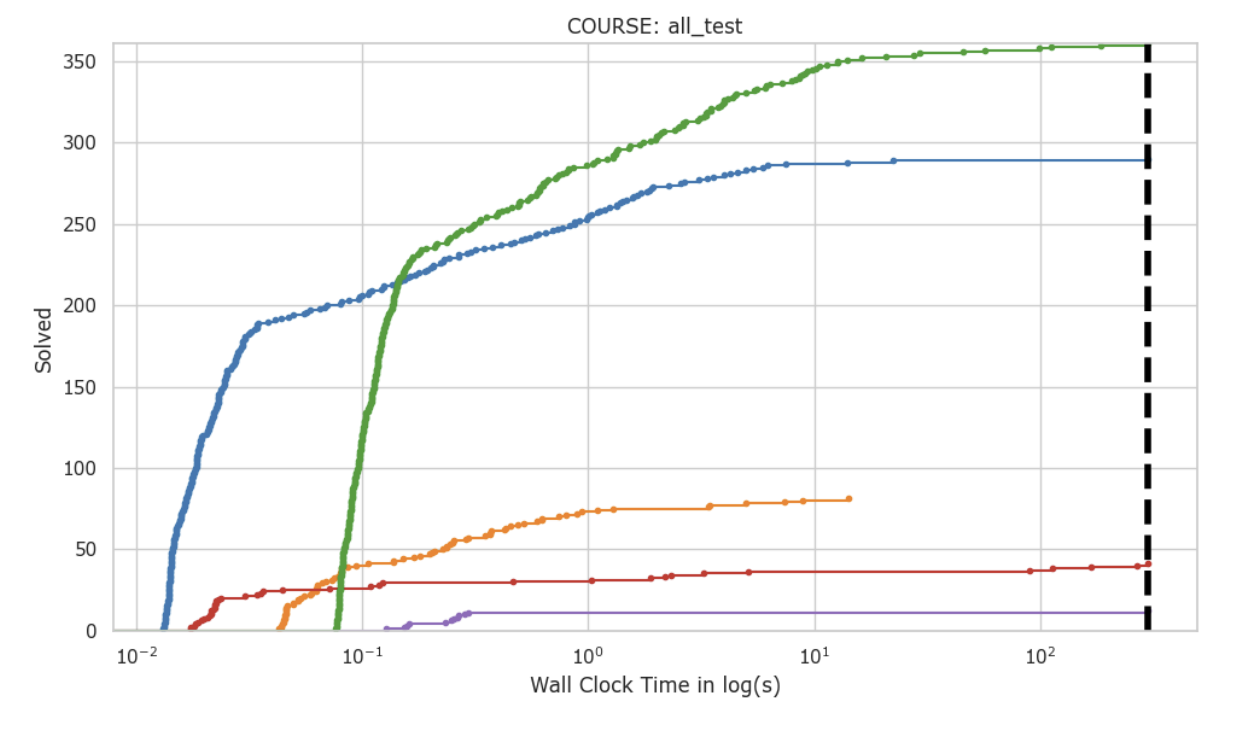
\includegraphics[width=0.6\textwidth]{all_test_course.png}
    \caption{Course: all\_test - Wall Clock Time vs Solved Instances}
    \label{fig:all_test_course}
\end{figure}

To better understand each algorithm’s performance across different categories, we organized the race into a set of courses. Each “course” is designed to test the algorithms in specific scenarios of the maximum matching problem, with a focus on different parameters like graph size, edge density, and matching characteristics. These courses simulate a variety of real-world and theoretical conditions, allowing us to isolate and examine distinct aspects of each algorithm’s behavior. By doing so, each course provides valuable insights into the relative effectiveness of the algorithms within that particular scenario.

Each course was developed to emphasize different graph characteristics based on the following parameters:

\begin{itemize}
    \item $d$: the number of partitions in the graph,
    \item $n$: the number of vertices,
    \item $m$: the number of edges, and
    \item $E$: the set of edges
    \item $M$: size of Maximum Matching
\end{itemize}

The courses that were studied are:
\begin{itemize}
    \item \textbf{Course 1: Perfect Matching} \\
    Tests solvers on graphs where every vertex can be matched.
    \item \textbf{Course 2: Random Matching (not perfect)} \\
    Uses graphs where perfect matching is not possible, highlighting algorithm behavior in imperfect matching situations.
    \item \textbf{Course 3: $\vert$Max-Matching$\vert$ in $[n/2,3n/4)$} \\
    Focuses on instances where the maximum matching is in the third quartile range.
    \item \textbf{Course 4: $\vert$Matching$\vert$ in $[3n/4, n-1]$} \\
    Instances where $\vert$Matching$\vert$ is in the fourth quartile, testing the solvers' efficiency on moderately large matching solutions.
    \item \textbf{Course 5: Large $n$ ($>1000$)} \\
    Evaluates solver performance on graphs with a large number of vertices, providing insight into scalability.
    \item \textbf{Course 6: Complete Graph} \\
    Examines algorithm efficiency on fully connected graphs.
    \item \textbf{Course 7: Large $m$ ($> \frac{n^d}{2}$) - Dense Graphs} \\
    Tests solvers on dense graphs where the number of edges $m$ exceeds half the maximum possible edges.
    \item \textbf{Course 8: Small $m$ ($< \frac{n^d}{2}$) - Sparse Graphs} \\
    Evaluates performance on sparse graphs, representing low-density structures.
    \item \textbf{Course 9: Easy problems with small $n$ and $m$ values} \\
    Provides a baseline with simpler problem instances with low vertex and edge counts.
\end{itemize}

Each course has specific values for the parameters listed above, allowing us to evaluate solver performance in different cases. By using a wide range of courses, we ensure that our evaluation is comprehensive and relevant to different types of maximum matching scenarios.\\
\\
Furthermore, we know that a bipartite matching problem runs in P whereas, for dimensions greater than 2, the problem is NP-hard. Thus, we split the algorithms into two categories: $d = 2$ and $d > 2$. This will better compare algorithms' performances by dividing them into P and NP problems.\\
\\
This evaluation framework is beneficial as it provides a deep understanding of solver performance. By analyzing algorithms under diverse conditions, we can make informed recommendations on which solver to use for different types of matching problems. The insights gained from these tests can guide the development of new, optimized algorithms for maximum matching problems, and help choose the best solver for specific use cases. The structure of courses and races allows for a robust comparison, ensuring that we can draw meaningful conclusions about each solver’s capabilities and limitations.
        \subsection{Performance Analysis}
        
Based on the courses discussed above, we measured each algorithm's ability to solve tests based on a selected timeout against the wall clock time (in $\log(s)$). This helps us analyze how many and how fast each algorithm can solve tests within the 5-minute timeout per test for $d>2$ solvers and 1-second timeout per test for $d=2$ solvers in each course. Moreover, measuring wall clock time in $\log(s)$ helps visualize data more effectively as the data points are distributed more evenly.  \\
These performance graphs are designed to provide an intuitive comparison of the algorithms. The closer each algorithm's performance line is to the y-axis, the faster the algorithm completes its tests, indicating a lower wall clock time. Additionally, the higher a line is on the graph, the more tests the algorithm successfully solved, showing its accuracy, and effectiveness. To evaluate overall performance, we consider both these aspects. A fast algorithm that can only solve a few tests could indicate that the algorithm got "lucky" with certain test cases. An accurate algorithm that is slow could suggest that it produces relatively better results while compromising speed.


\subsubsection*{Course 1: Perfect Matching}

\begin{figure}[h!]
    \centering
    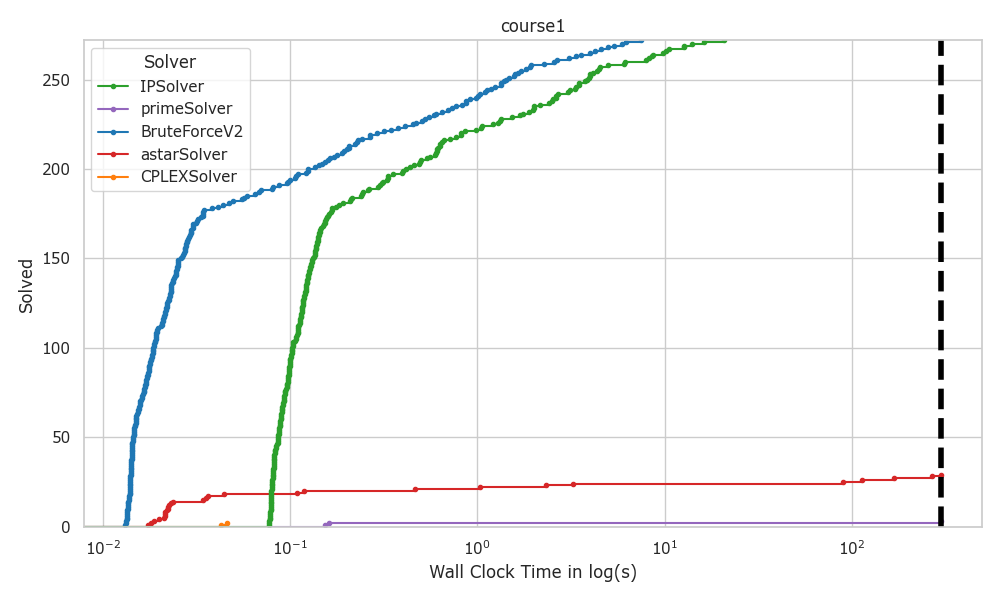
\includegraphics[width=\textwidth]{Graphs/course1.png}
    \caption{Performance of solvers on course 1}
\end{figure}

For course 1, the graph demonstrates clear differences in the performance of the solvers. The \textbf{BruteForceV2} solver, represented in blue, is both the fastest and the most accurate, solving all the tests within a shorter wall clock time. The \textbf{IPSolver}, shown in green, also solves a high number of tests, but it is slightly slower compared to BruteForceV2. Other solvers, such as \textbf{CPLEXSolver} (orange) and \textbf{primeSolver} (purple), perform very poorly as they were only able to solve a small fraction of the tests, and they were also not very fast on the tests they passed. The \textbf{astarSolver} (red) was able to solve more tests than CPLEXSolver and primeSolver but failed to compete with BruteForceV2 or IPSolver in both speed and accuracy. Overall, for a perfect matching scenario, BruteForceV2 demonstrates the best performance, followed closely by IPSolver, while the remaining solvers show limited efficiency in this course.

\subsubsection*{Course 2: Random Matching (non-perfect)}

\begin{figure}[h!]
    \centering
    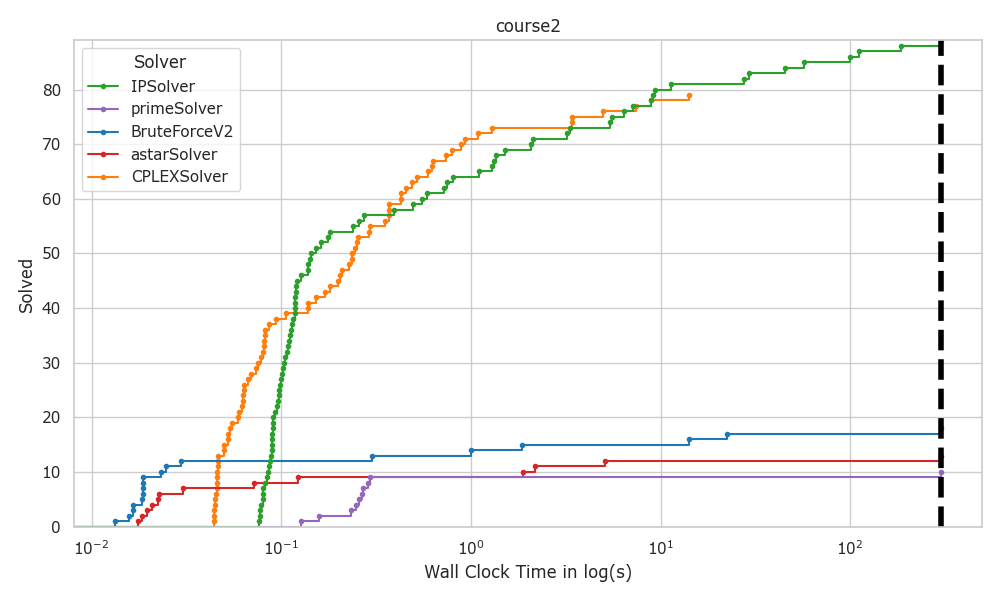
\includegraphics[width=\textwidth]{Graphs/course2.png}
    \caption{Performance of solvers on course 2}
\end{figure}

For course 2, the \textbf{IPSolver} (green) outperforms the others, solving the highest number of tests while also maintaining a relatively high speed. The \textbf{CPLEXSolver} (orange) also performs well, solving nearly as many tests as IPSolver, though it is slightly slower on some tests. The \textbf{BruteForceV2} (blue), while both accurate and fast on course 1, struggles in a non-perfect matching scenario, solving far fewer tests and taking considerably more time. Similarly, the \textbf{astarSolver} (red) and \textbf{primeSolver} (purple) also show limited performance, solving only a small fraction of tests with significantly slower speeds. Overall, for a non-perfect scenario, the IPSolver outperforms the other solvers, both in efficiency and effectiveness for course 2, with CPLEXSolver having a very similar performance.

\subsubsection*{Course 3: $\vert$Max-Matching$\vert$ in $[n/2,3n/4)$}

\begin{figure}[h!]
    \centering
    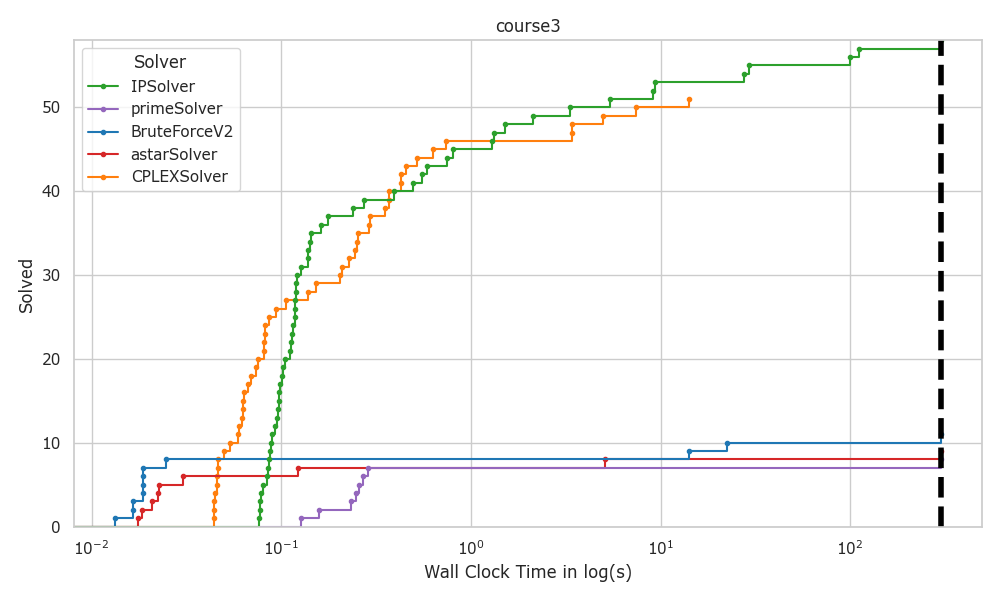
\includegraphics[width=\textwidth]{Graphs/course3.png}
    \caption{Performance of solvers on course 3}
\end{figure}

For course 3, the \textbf{IPSolver} (green) again performs better than other solvers, solving the highest number of tests while maintaining a low wall clock time. The \textbf{CPLEXSolver} (orange) closely follows IPSolver, solving a comparable number of tests at a similar speed. Thus, both solvers demonstrate strong accuracy and efficiency. Other solvers including \textbf{BruteForceV2} (blue), \textbf{astarSolver} (red) and \textbf{primeSolver} (purple) perform poorly, solving only a small number of tests with longer computation times. Overall, IPSolver and CPLEXSolver significantly outperform other solvers in both speed and effectiveness for course 3 where the size of matching lies in the fourth quartile.

\subsubsection*{Course 5: Large $n$ $(>1000)$}
\begin{figure}[h!]
    \centering
    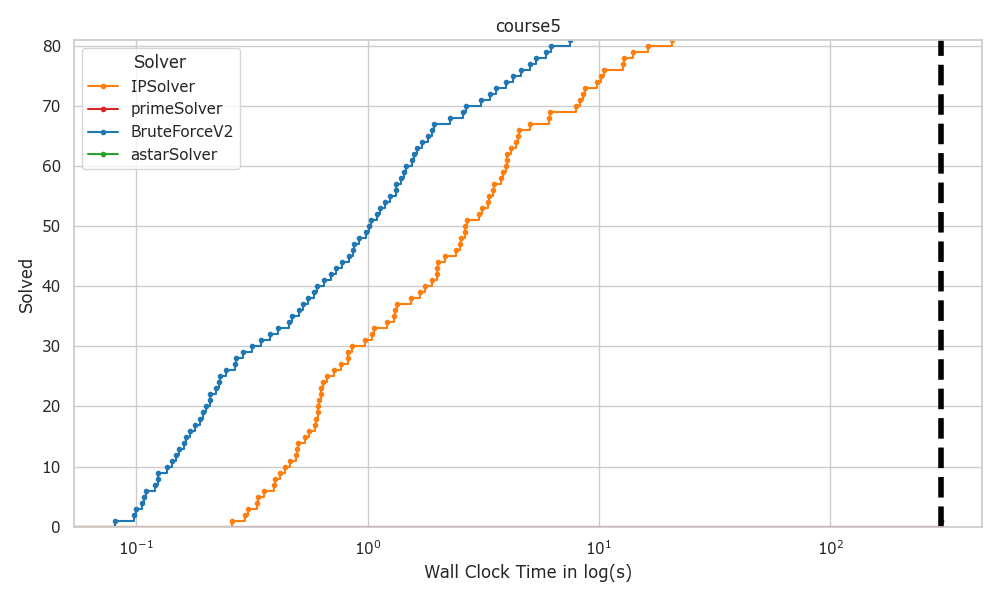
\includegraphics[width=\textwidth]{Graphs/course5.png}
    \caption{Performance of solvers on course 5}
\end{figure}

For course 5, we were only able to gather data for \textbf{BruteForceV2} (blue) and \textbf{IPSolver} (orange). Other solvers were not able to run any tests for large amounts of vertices within the 5-minute timeout. The BruteForceV2 solver performs slightly better compared to the IPSolver, however, their performances are very similar. Both were able to solve around 80 test cases within the timeout. However, this result is not fully reflective of the provided criteria as most of the tests that were generated had a perfect matching.  Overall, BruteForceV2 and IPSolver significantly outperform other solvers for course 5 where the graphs have a large size.

\subsubsection*{Course 8: Small $m$ ($< \frac{n^d}{2}$) - Sparse Graphs}

\begin{figure}[h!]
    \centering
    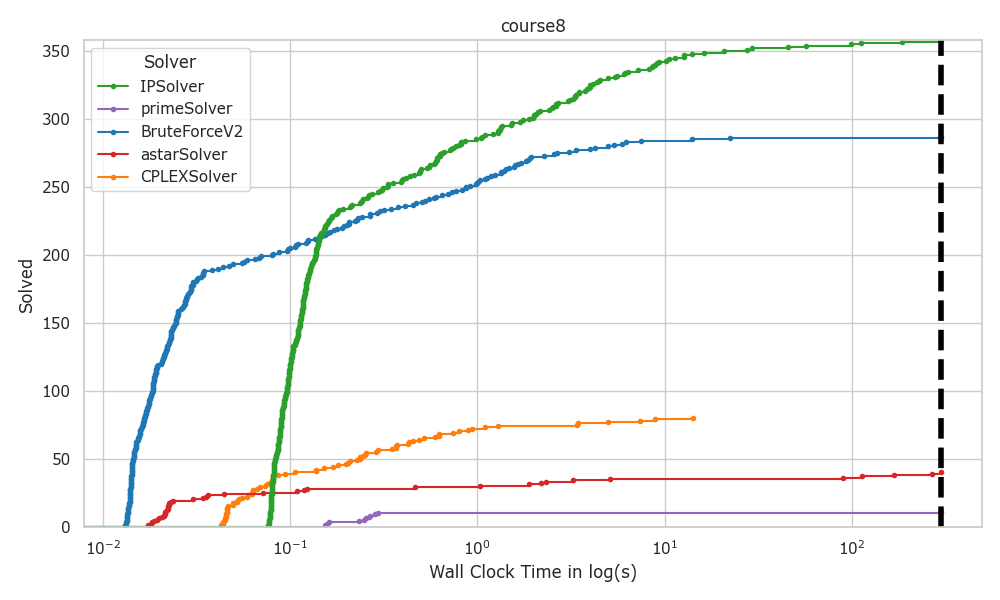
\includegraphics[width=\textwidth]{Graphs/course8.png}
    \caption{Performance of solvers on course 8}
\end{figure}

For course 8, the \textbf{IPSolver} (green) was able to solve the highest number of tests while maintaining a relatively low wall clock time. However, the \textbf{BruteForceV2} (blue) was able to solve around 200 test cases faster than the other solvers. Thus, both solvers demonstrate strong performance in this course. Other solvers including \textbf{astarSolver} (red), \textbf{CPLEXSolver} (orange) and \textbf{primeSolver} (purple) perform poorly in this course, solving only a small number of tests. Overall, IPSolver is more accurate than other solvers while the BruteForceV2 solver is faster for course 8 where the graphs are sparse and have a low number of edges.

\subsubsection*{Course 9: Easy problems with small $n$ $(<100)$ and $m$ $(<50)$ values}

\begin{figure}[h!]
    \centering
    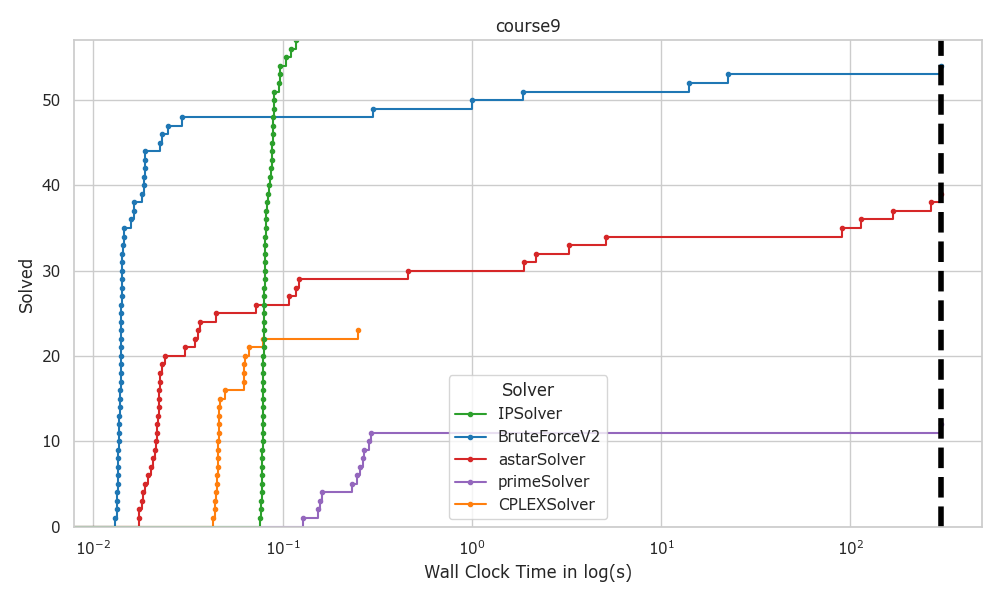
\includegraphics[width=\textwidth]{Graphs/course9.png}
    \caption{Performance of solvers on course 9}
\end{figure}

For course 9, the \textbf{BruteForceV2} (blue) and \textbf{IPSolver} (green) were able to solve the highest number of tests. However, due to the lack of test data, these graphs may not accurately reflect the true performance of the algorithms. Thus, more data would have given a more conclusive result for this course. Based on the results, the BruteForceV2 solver was the fastest with relatively higher accuracy while the IPSolver was the most accurate. Other solvers also performed well but failed to solve most of the test cases.


\subsubsection*{Overall Results}

Dividing Races into different courses allowed us to see how each algorithm behaves in different scenarios of the problem. Across all courses, the IPSolver consistently demonstrates strong performance, solving the highest number of tests in most scenarios while maintaining relatively low wall clock times. Moreover, it outperformed most of the other solvers in random matching (Course 2), larger size Max-Matching (Course 3,) and sparse graph scenarios (Course 8). Similarly, the BruteForceV2 solver demonstrates better performance on more structured problems like perfect matching (Course 1), large graphs (course 5), and easier problems (Course 9). However, it struggled with larger or more complex graph scenarios, like Course 2 and Course 3. The CPLEXSolver shows competitive performance in specific scenarios like random matching (Course 2) and large-sized matching (Course 3) but underperforms in other courses. Meanwhile, both the astarSolver and primeSolver are less competitive, solving significantly fewer tests across all courses and being slower compared to other solvers.


\subsubsection*{Limitations and Future Work}

One of the main limitations of this study is the inability to generate sufficient data, specifically for Courses 4, 6, and 7. Due to the complexity of generating test cases for these courses, we were unable to produce meaningful visualizations or comparisons for these scenarios. 

Another limitation lies in the relatively small number of test cases generated for some of the courses. A larger number of test cases, along with an increased timeout duration for computational experiments, would provide a better evaluation of solver performance, particularly for large graphs or highly complex scenarios. Additionally, the solvers might demonstrate different performances if tested over a broader range of problems and parameters.

In the future, we focus on refining the design of the courses by looking at multiple parameters to capture more details of solver performance. Moreover, having proper development tools to generate tests based on a specification will greatly benefit testing with a broader range of values. Overall, with more test data, improved parameter tuning, and enhanced tools for generating challenging scenarios, we can provide a deeper understanding of solver performance across diverse scenarios.

\chapter{Applications}
\label{sec:applications}
\input{practicalApplications.tex}
\chapter{Implementation}
\label{sec:implementation}

% Author @ Sam Appleton, IN_PROGRESS, Reviewer @ Jeremy Perez, Due Date 11/11

This chapter discusses our implementation in determining the difficulty of 
the Maximum Matching problem. This includes a summary of created programs,
an explanation of implemented solvers, our development tools, and a 
discussion on parallel programming. 

\section{Implementation}
Understanding the difficulty of Maximum Matching requires exploration via 
implementation. Our implementation includes various solvers and tools for answering
the question of Maximum Matching. In this section, we summarize and describe
each part of the implementation. 

Our implementation includes:
\begin{itemize}
	\item \textbf{Benchmarking}: Tools that determine the running time of 
    each solver algorithm. They take in a series of tests and a solver, and then
    return the correctness of the results and the wall-clock time of each solved test.
	\item \textbf{Solvers}: Algorithms that find the maximum matching on a given
    graph instance. They include many different types of solvers which implement
    different programming styles, such as integer programming and heuristics. 
	\item \textbf{Test Generators}: Tools for creating graph instances. They 
    generate random graphs with known maximum matchings for the sake of testing 
    correctness and efficiency. 
	\item \textbf{Visualizer}: Tool for creating visual representations of
    graph instances. It provides access for humans to interpret the graph objects,
    which are hard to easily understand. 
\end{itemize}

\section{Benchmarking} \label{BenchmarkingSummary}
Benchmarking is crucial to our implementation. It allows us to determine the efficiency 
of our solvers, thus giving an empirical way of comparing solvers. 
Our benchmarking tool takes in a series of graphs and runs each of them against a solver that
finds the maximum matching on each graph.
It then determines the accuracy of the solver by comparing the returned maximum matching and 
seeing if it is valid. It also records the wall-clock time needed for each graph
in the input to compare the running times of each solver. Each graph is represented 
in a .mmi (Maximum Matching Instance) file, and the files paths to each graph 
is stored in a .mmb (Maximum Matching Benchmarking) file. This allows .mmb files to be created
with specific factors in mind, such as only containing dense graphs with $d > 2$. This program
is essential to our understanding of the hardness of Maximum Matching as it gives a 
quantifiable determinant of difficulty, that being the actual time it take to solve a given 
instance of the problem. Calculating running time on the same machine with the same environment
allows us to easily compare different implementations. 

A .mmi file contains a single graph object as represented by the following lines:
\begin{enumerate}
	\item $d$, an integer that represents the number of dimension in the graph. 
	\item $n$, an integer that represent the number of vertices in each dimension.
	\item $m$, an integer that represents the number of edges in the graph.
	\item $m$ tuples of length $d$ that contain numbers $(1..n)$ that represent
	each edge on the graph.
	\item $M$, an integer that represents the cardinality of the known maximum matching 
    of the graph. Note that this line is optional.
\end{enumerate}
Figure \ref{fig:exampleMMi} contains an example .mmi file, and Figure \ref{fig:d4v5} contains 
a visualization of the corresponding output.

\begin{figure}[t!]
    \centering
    \begin{minipage}{0.45\textwidth}
        \centering
        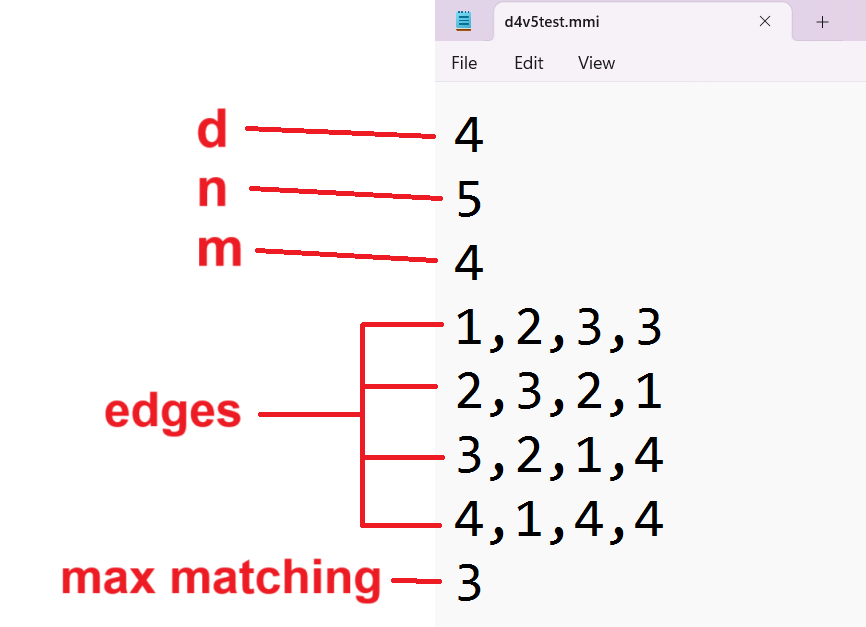
\includegraphics[width=\textwidth]{images/exampleMMI.png}
        \caption{An example of an .mmi instance. Each line is labeled with the information
        it contains. Note that the file represents some information that is not stated by 
        just the edges, such as the fact there is a 5th row of vertices that no edge visits.}
        \label{fig:exampleMMi}
    \end{minipage}
    \hfill
\end{figure}

\begin{figure}[t!]
    \centering
    \begin{minipage}{0.45\textwidth}
        \centering
        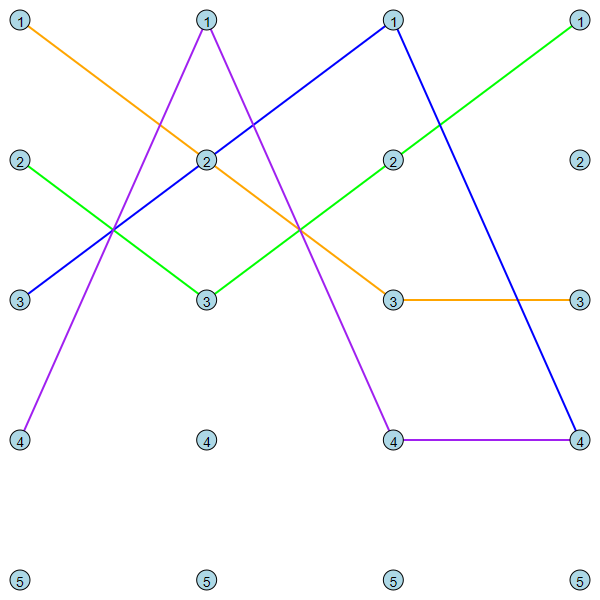
\includegraphics[width=\textwidth]{images/d4v5test.png}
        \caption{An example of a graph represented in a .mmi file.}
        \label{fig:d4v5}
    \end{minipage}
    \hfill
\end{figure}

A .mmb files contains a series of paths to .mmi files. Each line contains a path to 
a .mmi file or a series of .mmi files. Note that .mmb supports wildcards, which are
represented as a *. This means that one line in .mmb file can lead to many 
different .mmi files. This is useful for including all .mmi files in a folder,
which is often the case for test suites. 

\section{Solvers} \label{SolverSummary}
There are many solvers in our implementation. Each solver takes in a graph instance
as described in Section \ref{BenchmarkingSummary} and returns a list of edges representing
a maximum matching on the graph instance. We implement many different algorithms and 
programming styles to find efficient ways of finding the maximum matching. 
The following is a list of the
different types of solver implemented over the course of the project:
\begin{itemize}
    \item Edmonds-Karp 
    \item Hopcroft-Karp
    \item Brute Force
    \item A*
    \item Depth First Search
    \item Integer Programming
    \item Parallel Programming
    \item Approximate solvers
\end{itemize}
For more information on the implementation of solvers and an example of an implemented solver,
see Section \ref{ekImplement}.

\section{Test Generators}
Each solver needs to be tested against a large variety of .mmi files. This is
done to determine not only the accuracy, but also the running time. There are 
currently two test generators in our implementation: a Brute Force verified 
generator, and a strategic $d > 2$ generator. For more details, see Section \ref{StrategicRandomTest}. Each generator provides
a way to randomly generate graphs with known maximum matching sizes. We compare 
the cardinality of the set of edges returned by each solver to the known cardinality of
the maximum matching to
determine accuracy. Being able to produce large groups of graphs also allows for 
diverse test suites to be generated. We then generate courses
for determining running time using the benchmarking programs, as seen in 
Section \ref{BenchmarkingSummary}. 

\section{Visualizer}
A visualizer allows for .mmi files to be more easily understandable to a human 
audience. The visualizer utilizes the graph framework provided for by igraph and 
pycairo. Each visualization is a .png that represents each dimension as a column with each vertex of the same value on the same row. Hyperedges are represented by
different color lines for ease of recognition.

The visualizer visualizes graphs by parsing a .mmi file and then converting the information
into a pycario graph object. Note that pycario does not support d-partite graphs or hyperedges,
so the visualizer adds vertices and edges to the graph object to emulate them.

\begin{figure}[t!]
    \centering
    \begin{minipage}{0.45\textwidth}
        \centering
        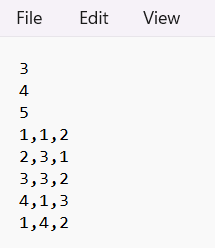
\includegraphics[width=\textwidth]{images/exampleviz.png}
        \caption{An example .mmi file to visualize.}
        \label{fig:vizbase}
    \end{minipage}
    \hfill
\end{figure}

\begin{figure}[t!]
    \centering
    \begin{minipage}{0.45\textwidth}
        \centering
        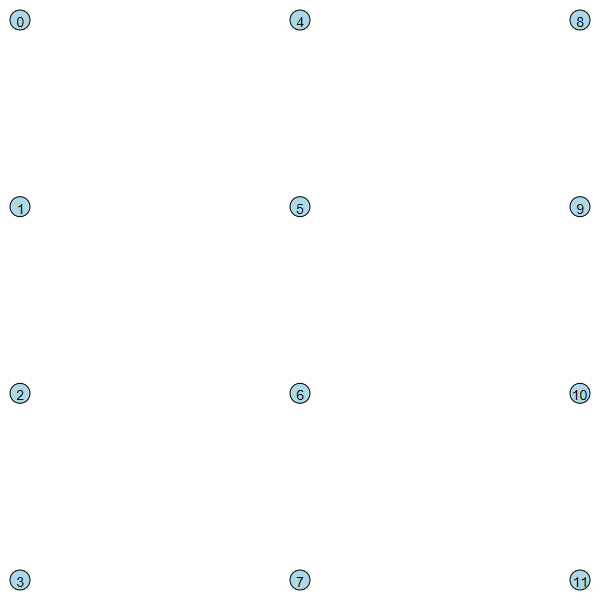
\includegraphics[width=\textwidth]{images/viz0.png}
        \caption{An example of how nodes are actually represented in the pycairo graph object in the visualizer. Note how nodes are labeled starting from 0 and increasing by 1. Uses the information given in Figure \ref{fig:vizbase}}
        \label{fig:viz0}
    \end{minipage}
    \hfill
\end{figure}

First, the visualizer adds $d * n$ edges to the graph object. Pycario automatically adds 
labels to the vertices in order of their addition starting at 0. This is shown in Figure
\ref{fig:viz0}. We add custom labels to each vertex using the formula 
$new label$ $=(label \% n) + 1$. This can be seen in Figure \ref{fig:viz1}.

\begin{figure}[t!]
    \centering
    \begin{minipage}{0.45\textwidth}
        \centering
        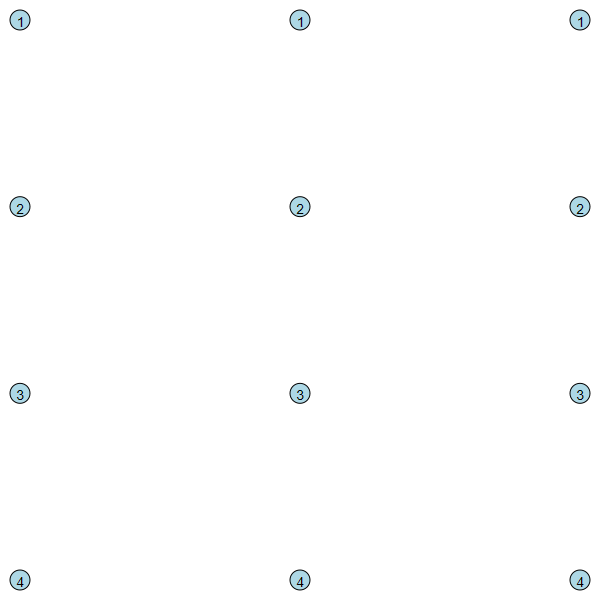
\includegraphics[width=\textwidth]{images/viz1.png}
        \caption{An example of how vertices are labeled in the visualizer. Continues from Figure \ref{fig:viz0}}
        \label{fig:viz1}
    \end{minipage}
    \hfill
\end{figure}

Edges are added in a similar manner. We add a hyperedge $e$ one edge at a time. We do this by 
adding edges using the formula $(((e[i] - 1) + n * i), ((e[i+1] - 1) + n * (i + 1)))$. We 
subtract 1 from the value at each index as pycario stores labels starting at 0, but we store
vertices starting from 1 in the .mmi file. We then add the $n * i$ to each vertex to 
place it in the correct dimension. This is seen in Figure \ref{fig:viz2}

\begin{figure}[t!]
    \centering
    \begin{minipage}{0.45\textwidth}
        \centering
        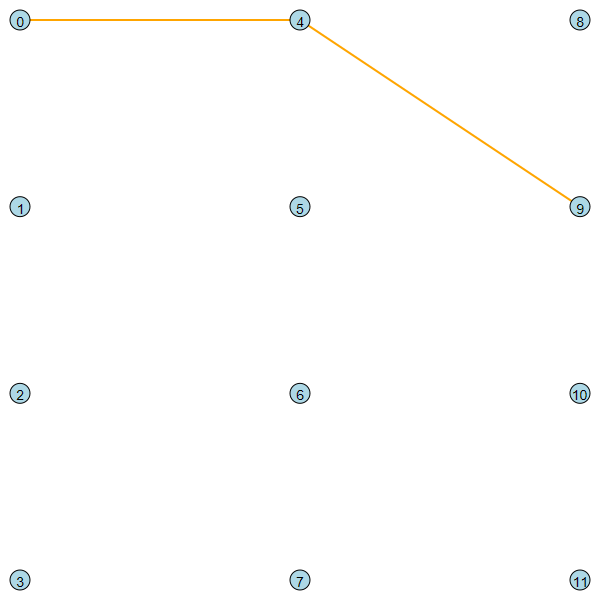
\includegraphics[width=\textwidth]{images/viz2.png}
        \caption{An example of how a single hyperedge is added to the visual. In this case, we are adding the hyper edge $(1, 1, 2)$. Using the formula, we first add the edge $(((e[0] - 1) + 4 * 0), ((e[0+1] - 1) + 4 * (0 + 1)))$. This gives us $((0 + 0), (0 + 4))$ or $(0,4)$. We then add the next edge in the hyperedge $(((e[1] - 1) + 4 * 1), ((e[1+1] - 1) + 4 * (1 + 1)))$ or $(4), (8)$. We then color the edges accordingly to represent the hyperedge.}
        \label{fig:viz2}
    \end{minipage}
    \hfill
\end{figure}

For ease of visual clarity, we also keep track of how many edges are represented in the 
hyperedge so that they can be colored accordingly. We repeat this for each hyperedge until 
there are no more hyperedges to draw as seen in Figure \ref{fig:viz3}.

\begin{figure}[t!]
    \centering
    \begin{minipage}{0.45\textwidth}
        \centering
        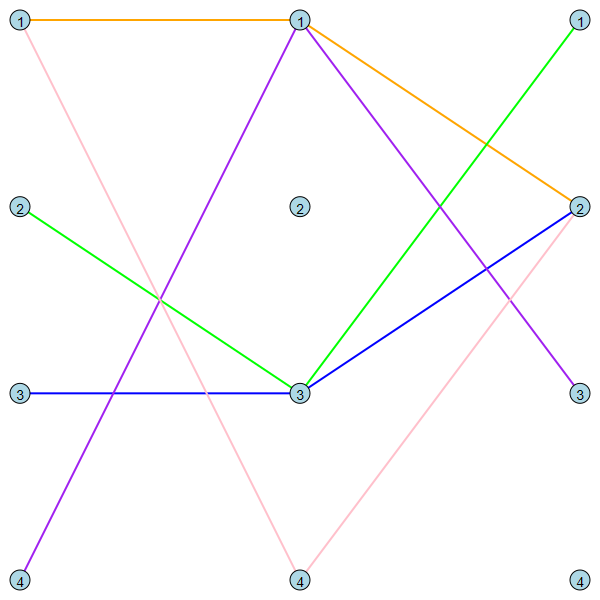
\includegraphics[width=\textwidth]{images/viz3.png}
        \caption{A completed visualization of Figure \ref{fig:vizbase}}
        \label{fig:viz3}
    \end{minipage}
    \hfill
\end{figure}


\section{Brute-Force}

\subsubsection*{Introduction}
The Brute Force algorithm for d-partite matching works by exhaustively searching through all possible subsets of edges within the graph, identifying the largest subset that forms a valid matching. This approach guarantees that the maximum matching is found, as it explores every possible combination of edges. However, it is computationally intensive and becomes increasingly impractical for large graphs due to the sheer number of edge subsets to evaluate.

\subsubsection*{Algorithm:}
The Brute Force algorithm follows these steps to identify the maximum matching:

\begin{enumerate}

    \item \textbf{Iterate Through All Edge Subsets}: For every possible subset of edges (from size \( n \) to 1):
    \begin{itemize}
        \item \textbf{Check for Valid Matching}: Determine if the current subset of edges forms a valid matching by ensuring no two edges in the subset share a common vertex.
        \item \textbf{Stop at the first Maximum Matching}: If the current subset forms a valid matching then, that is the solution of the problem.
    \end{itemize}
    \item \textbf{Return the Largest Valid Subset}: Examine all subsets from $n$ to 1 until the first matching is found, and return that subset which forms a valid matching.
\end{enumerate}

This exhaustive search approach ensures that the largest possible matching is found, making it an accurate but computationally expensive method.

\subsubsection*{Checking if an Edge is Valid in the Matching Set:}
To determine whether a subset of edges forms a valid matching, each edge must satisfy the requirement that no two edges in the matching share a vertex. This criterion can be tracked using a two-dimensional array, \texttt{d\_table}, which helps ensure that no vertices are repeated across different edges in the subset:

\begin{itemize}
    \item \textbf{Criteria for a Valid Edge}: No two edges in the matching can share a vertex.
    \item \textbf{Tracking Shared Vertices}: Initialize \texttt{d\_table} as a list of lists: \texttt{d\_table = [ [], [], [], ... ]} with \( d \) empty lists.
    \begin{itemize}
        \item Each list \texttt{d\_table[i]} represents the vertices in the \( i \)th dimension or column of the d-partite graph.
        \item As edges are evaluated, \texttt{d\_table} keeps track of vertices included in each dimension to avoid overlaps.
    \end{itemize}
\end{itemize}

This approach ensures that each subset is correctly validated, though it adds to the computational overhead due to constant updates and checks on the \texttt{d\_table}.

\newpage

\subsection*{Brute Force Solver Pseudocode}

\begin{algorithm}
\caption{Brute Force Solver}
\begin{algorithmic}[1]
\STATE \textbf{Input:} Graph $G$ with dimensions $d$, vertices $n$, edges $m$, and edge set $E$
\STATE \textbf{Output:} Maximum matching subset of edges

\FOR{$r \gets n$ \textbf{down to} $1$}
    \FOR{each subset $\textit{edge\_comb}$ of size $r$ from $E$}
        \IF{$\textit{is\_valid\_combination}(\textit{edge\_comb}, d)$}
            \RETURN $\textit{edge\_comb}$ \hfill // Return valid matching immediately
        \ENDIF
    \ENDFOR
\ENDFOR
\RETURN $[]$ \hfill // Return empty list if no matching found
\end{algorithmic}
\end{algorithm}

% \subsection*{is\_valid\_combination Function Pseudocode}

\begin{algorithm}
\caption{is\_valid\_combination}
\begin{algorithmic}
\STATE \textbf{Input:} Edge combination $\textit{edge\_comb}$, dimension $d$
\STATE Initialize $d\_table \gets [\{\}, \{\}, \dots, \{\}]$ (an array of $d$ empty sets)
\FOR{each edge $e$ in $\textit{edge\_comb}$}
    \FOR{$i \gets 1$ \textbf{to} $d$}
        \IF{$e[i]$ is in $d\_table[i]$}
            \RETURN \textbf{False} \hfill // Invalid if vertex is already used
        \ENDIF
        \STATE Add $e[i]$ to $d\_table[i]$
    \ENDFOR
\ENDFOR
\RETURN \textbf{True} \hfill // Valid matching if no vertices overlap
\end{algorithmic}
\end{algorithm}



\subsubsection*{Example:}


Consider a simple example where:
\[
d = 2, \quad n = 3, \quad m = 4, \quad E = \{ [1, 1], [2, 1], [3, 2], [3, 3] \}
\]

\begin{center}
\begin{tikzpicture}
    % Define nodes for two sets
    \node[circle, draw] (A1) at (0, 1) {1};
    \node[circle, draw] (A2) at (0, 0) {2};
    \node[circle, draw] (A3) at (0, -1) {3};

    \node[circle, draw] (B1) at (3, 1) {1};
    \node[circle, draw] (B2) at (3, 0) {2};
    \node[circle, draw] (B3) at (3, -1) {3};

    % Draw edges
    \draw (A1) -- (B1) node[midway, above] {};
    \draw (A2) -- (B1) node[midway, above] {};
    \draw (A3) -- (B2) node[midway, above] {};
    \draw (A3) -- (B3) node[midway, above] {};

\end{tikzpicture}
\end{center}
\begin{center}
    \textbf{Figure:} The Graph representation of the problem above
\end{center}

The brute force algorithm examines all possible subsets of edges from size \( n \) down to 1 and picks the first valid matching.


\paragraph{All Possible Subsets of edges:}
\begin{itemize}
    \item Size 1: \([1, 1], [2, 1], [3, 2], [3, 3]\)
    \item Size 2: \(\{[1, 1], [2, 1]\}, \{[1, 1], [3, 2]\}, \{[1, 1], [3, 3]\}, \{[2, 1], [3, 2]\}, \{[2, 1], [3, 3]\}, \{[3, 2], [3, 3]\}\)
    \item Size 3: \(\{[1, 1], [2, 1], [3, 2]\}, \{[1, 1], [2, 1], [3, 3]\}, \{[1, 1], [3, 2], [3, 3]\}, \{[2, 1], [3, 2], [3, 3]\}\)
\end{itemize}

Initially, the algorithm will iterate through all subsets of size $n=3$ to see if any subset forms a valid matching. In this example, no subset of size 3 forms a valid matching, thus, the algorithm will then check for subsets of size $n-1 = 2$. The subset $\{[1, 1], [3, 2]\}$ forms a valid matching. Hence, it will return this subset as the solution to this problem.


\begin{center}
\begin{tikzpicture}
    % Define nodes for two sets
    \node[circle, draw] (A1) at (0, 1) {1};
    \node[circle, draw] (A2) at (0, 0) {2};
    \node[circle, draw] (A3) at (0, -1) {3};

    \node[circle, draw] (B1) at (3, 1) {1};
    \node[circle, draw] (B2) at (3, 0) {2};
    \node[circle, draw] (B3) at (3, -1) {3};

    % Draw edges
    \draw[green, thick] (A1) -- (B1) node[midway, above] {};
    \draw (A2) -- (B1) node[midway, above] {};
    \draw[green, thick] (A3) -- (B2) node[midway, above] {};
    \draw (A3) -- (B3) node[midway, above] {};

\end{tikzpicture}

\end{center}
\begin{center}
    \textbf{Figure:} Solution to the above problem, with $Matching =$ \(\{[1, 1], [3, 2]\}\) highlighted in green.
\end{center}


This example demonstrates how the brute force algorithm systematically examines each subset of edges to identify a valid matching.

\subsubsection*{Complexity:}
The complexity of this algorithm can be estimated through the choices made by the algorithm. The maximum matching size can be up to $n$, which is given by the set of edges that form a valid matching. Thus, in the worst case, the algorithm looks through all possible combinations of $m$ edges from size $n$ to $1$ for all the vertices. Moreover, the maximum number of edges is a graph is $m=n^d$. Hence the \textbf{worst-case run time} can be given by the equation:
\[
\sum_{i=0}^{n} \binom{m}{i} \cdot n \leq n \cdot \binom{n^d}{n}  \cdot n \leq n^2 \cdot \frac{(n^d)^n}{n!} \leq n^2 \cdot \frac{(n^d)^n}{n^n} \leq n^2 \cdot (n^{d-1})^n
\]

\subsubsection*{Advantages and Disadvantages:}
The Brute Force algorithm is versatile and can be applied to graphs of arbitrary dimensions, not just \( d = 2 \). Its main advantage is that it guarantees the maximum matching, as it evaluates every possible edge combination. Thus, it is a reliable choice when exact solutions are essential. For example, a lot of the test cases which was used to check the other algorithms were created using the Brute Force Algorithm. \\
\\
The main drawback of the Brute Force approach is its high computational cost. It quickly becomes impractical for larger graphs due to the exponential number of edge subsets that need to be evaluated. Even with optimization techniques like early termination and approximation, this method remains slow and resource-intensive.\\
\\
In summary, the Brute Force algorithm offers a guaranteed approach to finding the maximum matching in d-partite graphs. However, its computational demands make it best suited for smaller or simpler graphs. For larger, more complex graphs, alternative algorithms or optimization strategies are generally preferred. Nevertheless, the Brute Force approach remains a valuable tool, especially for generating test cases and validating the effectiveness of other matching algorithms.

\section{Bipartite Graph}
\label{sec:bipartite_graph_implementation}

% Author @ Huyen Tran, DONE

\subsection{Edmonds-Karp Implementation} \label{ekImplement}

In this implementation, the \texttt{MaxMatchingBipartite} class inherits from an abstract \texttt{Solver} class to compute the maximum matching in a bipartite graph using the \textbf{Edmonds-Karp algorithm}, introduced in section \ref{ek algo}. This approach utilizes a breadth-first search (BFS) to find augmenting paths in a flow network representation of the bipartite graph. Key elements and methods include:

\paragraph{Initialization}: The program begins by initializing the graph representation and setting up the residual graph. The \texttt{solve()} function accepts a graph instance \( G = (d, n, m, E) \). The residual graph is initialized as a nested dictionary, where capacities are assigned as follows: the source node is connected to each left vertex (set \( U \)) with unit capacity, the sink node is connected to each right vertex (set \( V \)) with unit capacity, and edges between sets \( U \) and \( V \) are assigned unit capacities based on the edges in \( E \).

\paragraph{Edmonds-Karp Algorithm Execution:} The algorithm is implemented by iteratively finding augmenting paths in the residual graph and adjusting capacities until no augmenting paths remain. Each iteration begins with a breadth-first search (BFS) from the source node to the sink node. The BFS explores the graph layer by layer, ensuring that the shortest path in terms of edge count is identified whenever an augmenting path exists. If an augmenting path is discovered, the program calculates the minimum residual capacity along this path, which determines the flow that can be pushed through. The \texttt{augment\_path()} function updates the residual graph by reducing capacities along forward edges and increasing capacities along reverse edges for this flow. These updates maintain the integrity of the flow network and prepare the graph for the next iteration. The process repeats until BFS fails to find an augmenting path, at which point the residual graph represents the final maximum flow.

\paragraph{Finding Augmenting Paths (BFS):} The process of finding augmenting paths in the residual graph is performed by the \texttt{BFS()} function, which uses breadth-first search to identify paths from the source to the sink that have positive residual capacity. This search begins by initializing the source node, marking it as visited, and adding it to a queue. The function maintains two dictionaries: one to record the distance of each node from the source, and another to track the previous vertex along the path. As BFS progresses, it explores adjacent vertices of the current node, checking whether the residual capacity of each edge is greater than zero and whether the adjacent vertex has not yet been visited. If these conditions are satisfied, the adjacent vertex is marked as visited, its distance from the source is updated, and its previous vertex is set to the current node. This vertex is then enqueued for further exploration. When the sink node is reached, the BFS halts and returns \texttt{True}, indicating the presence of an augmenting path. If the BFS completes without reaching the sink, the function returns \texttt{False}, signaling that no further augmenting paths exist. 

\paragraph{Flow Augmentation}: The flow augmentation process is carried out by the \texttt{augment\_path()} function, which updates the residual graph along the augmenting path found by the \texttt{BFS()} function. This process begins by identifying the minimum residual capacity along the augmenting path, which represents the maximum flow that can be pushed through this path without exceeding the capacities of any edge. To determine this minimum capacity, the function traces the path backward from the sink to the source using the dictionary of previous vertices populated during BFS. At each step, the residual capacity of the edge is compared to the current minimum flow, and the smallest value is retained. \\
Once the minimum capacity is identified, the function updates the residual graph by decreasing the capacities along the forward edges of the path by this flow value and increasing the capacities along the reverse edges by the same value. These updates ensure that the residual graph reflects the adjusted flow network, where the forward edges represent the remaining available capacity and the reverse edges allow for the possibility of reducing flow in subsequent iterations if necessary. The flow value for this augmenting path is added to the total flow of the graph, incrementally building towards the maximum flow. This iterative augmentation continues until no further augmenting paths can be found. 

\paragraph{Extracting the Matching}
After completing the flow augmentation process, the maximum matching is extracted from the residual graph. This step involves examining the edges in the bipartite graph to identify pairs of vertices that form the matching. The program iterates through the residual capacity of each reverse edge (from \( V \) to \( U \)) in the residual graph. A positive residual capacity on this reverse edge indicates that the edge was part of the flow in the original graph, signifying a matched pair. This matching is returned as a tuple of $n$-edges representing the maximum matching.\\

\noindent By using BFS to find shortest augmenting paths, the algorithm efficiently finds maximum matching in polynomial time. The separation of \texttt{BFS()} and \texttt{augment\_path()} functions simplifies the flow augmentation process, while the nested dictionary structure allows flexible updates of residual capacities.




% @author Huyen Tran, DONE
\subsection{Perfect Matching via Gaussian Elimination Implementation} \label{pmReduction}

In this implementation, the \texttt{PMBipartite} class inherits from an abstract \texttt{Solver} class to compute the perfect matching in a bipartite graph using the \textbf{Simple-Bipartite-Matching algorithm}, introduced in section \ref{matrix-perfect-matching}. This approach uses a matrix-based reduction to iteratively identify and refine matchings by using the ske-symmetric adjacency matrix to represent the graph's edges. The algorithm combines matrix inversion with the Schur complement to update the adjacency matrix efficiently. 

\paragraph{Matrix Construction:}
The \texttt{graph\_to\_adj} function takes the input graph \( G = (d, n, m, E) \) and generates a skew-symmetric adjacency matrix \( \tilde{A}(G) \), where \( \tilde{A}(G) \) has the block format:
\[
\tilde{A}(G) =
\begin{bmatrix}
0 & A_{12} \\
-A_{12}^T & 0
\end{bmatrix}.
\]
Since we only consider bipartite graphs, any non-zero entry \( A_{ij} \neq 0 \) in \( A_{12} \) or \( -A_{12}^T \) represents the same edge. For efficient implementation, the program directly constructs \( A = A_{12} \), assigning random weights \( x_{ij} \) for edges \( (i, j) \in E \). Specifically, \( A_{ij} = x_{ij} \) for \( i < j \) and \( A_{ij} = -x_{ij} \) for \( i > j \). Random weights are chosen uniquely from a sufficiently large range to minimize collisions and ensure stability during matrix inversion.

\paragraph{Matrix-Based Matching:}
After constructing the adjacency matrix \( A \), the inverse \( B = A^{-1} \) is computed. Non-zero entries in \( B \) indicate potential matching edges. The program iterates through each column \( c \) to identify an allowed edge. It examines the \( c \)-th column of \( B \) for a row \( r \) such that \( B[r, c] \neq 0 \) and  \( A[c, r] \neq 0 \) to ensure that we only consider edge exists in the original graph \( G \). Then, the edge \( (v, u) = (c, r) \) is added to the matching set \( M \), and the program proceeds to update the matrix \( B \).

\paragraph{Matrix Update Using the Schur Complement:}
When a valid edge \( (v, u) \) is selected, the matrix \( B \) is updated using the Schur complement to reduce the influence of the matched edge. The update formula is:
\[
B' = B - \frac{\mathbf{u} \mathbf{v}^T}{B[v, u]},
\]
where \( \mathbf{u} \) is the column vector corresponding to \( u \), and \( \mathbf{v} \) is the row vector corresponding to \( v \). After applying the Schur complement, the \( v \)-th row and \( u \)-th column are cleared by setting them to zero, effectively removing the matched vertices from further consideration.

\paragraph{Matching Extraction:}
The iterative process continues until all vertices are matched (\( |M| = n \)) or no valid edges remain in \( B \). The final matching \( M \) is extracted as a set of edges covering all vertices in the bipartite graph. If the algorithm does not find a perfect matching within the given number of iterations, it terminates without a result.

\paragraph{Randomized Approach and Repeated Attempts:}
Because random weights are used to construct \( A \), the performance of the algorithm can vary across runs. To address this variability, the implementation includes a retry mechanism that runs the algorithm multiple times (up to a maximum number of attempts or a time limit) until a perfect matching is found. This approach increases the likelihood of success while maintaining overall efficiency.\\

\noindent The use of skew-symmetric matrices and random weights ensures that the algorithm can efficiently handle dense bipartite graphs. By iteratively refining \( B \) using the Schur complement, the algorithm avoids traversing graph edges directly and instead leverages fast matrix operations. The complexity is \( O(n^\omega) \), where \( \omega \) is the matrix multiplication exponent, making the method computationally efficient for large-scale problems. The use of random weights in \( A \) introduces variability in performance, as the success of the algorithm depends on \( A \) being invertible. Dense bipartite graphs improve the likelihood of obtaining an invertible matrix, as the larger number of edges leads to a more populated \( A \), reducing the chances of linear dependence among rows or columns. This makes the algorithm particularly effective for dense graphs, where it performs better both in terms of runtime and consistency.





\section{Parallel Programming}
% Ethan O'Farrell, COMPLETE, Reviewer Jack Rubin, DUE DATE: 11/19

\textbf{Threading \& Parallel Programming}

\paragraph{}
\textbf{Parallel programming}, parallel processing, and parallel computing all refer to the concept 

of using computational resources to run different parts of a program in parallel. 

\textbf{Threading}Threading is a form of parallel programming which uses a shared memory space 

within a larger program. 


\subsubsection*{What is the purpose of threading?}


\paragraph{}
Threading serves as a practical way to improve algorithm runtime. Given an algorithm that 

runs in $O(n)$. The best possible improvement we can make to the runtime with threading is 

$O(s+(n/t)$ where $s$ is the fixed time to initialize and end the threads, and $t$ is the 

number of threads used. Of course, the runtime class cannot actually be improved, since 

$O(s+(n/t)$ is still absorbed by $O(n)$. However, this improvement can still greatly benefit 

the practical runtime. For example, given an algorithm that takes $30$ minutes for some $n$ 

size input to run. Altering the program to utilize a system that can handle 8 threads can 

reduce the runtime to under just $4$ minutes. 


\subsubsection*{How does threading relate to Maximum Matching?}


\paragraph{}
Parallel programming strategies generally rely on $1$ key concept: Memory Management. Whether 

or not the parallel parts of the program share a memory space will determine the best 

implementation. Threading benefits from a shared memory space, whereas processes split the 

program into disjoint memory spaces. So when do we use threading versus processes? Generally 

the following rules should be considered when deciding to use threading:


\begin{enumerate}

    \item Can the program be split into smaller programs?
    
    \item Does the order in which these programs run matter?
    
    \item Do the parallel parts of the program share information?

\end{enumerate}


\paragraph{}
Naturally, if the program can only be run sequentially, any form of parallel programming will be 

futile. In order to use threading, the program must be able to run multiple functions at the same 

time. If the order in which the results of parallel functions return matters, then synchronization

is required. For example, say we write a program that solves mathematical equations using PEMDAS. 

If we were to incorporate different threads for addition, subtraction, multiplication, division, 

etc., the order in which each thread computes its part of the equation matters. 


\paragraph{}
Synchronization is especially important when using shared memory spaces. Maximum Matching algorithms 

involve edges matching between various partitions of vertices. Such graphs are a form of shared 

memory. Therefore, when algorithms such as FordFulkerson and EdmondsKarp read and alter various parts 

of the graph, future searches will depend on these changes. Even a brute force approach involves a 

shared memory space. Usually brute force approaches utilize the construction of all subsets of edges

in the given graph. This collection of subsets can also be considered a shared memory space. 


\paragraph{}
The difference between brute force and traditional maximum matching algorithms is how these shared 

memory spaces are used. In the case of graph traversal algorithms, synchronization is necessary for

ensuring that multiple threads do not apply conflicting changes to the same graph at the same time. 

Whereas a brute force algorithm does not entail editing or searching of graphs, but rather adding new 

subsets to a single larger set. 


\subsubsection*{Synchronization}


\paragraph{}
As mentioned before, threading involves the use of a shared memory space. Usually, programmers 

avoid giving multiple sections of a program access to the same variable to avoid side effects. 

However, completely avoiding shared variables in parallel programs would involve a ton of copying. 

Not only is repeatedly cloning such variables a waste of memory space, we also lose most of the runtime

we gain from using threading in the first place. In order to solve this problem, we can employ the 

concept of synchronization to manage the access threads have in the shared memory space. In short,

by "synchronizing" the threads, we can ensure no $2$ threads access and alter the same variables 

at the same time. 


\paragraph{}
A common tool used for synchronization is called a semaphore. In short, we can think of semaphores

like a counting variable. Semaphores track how many threads are accessing or waiting to access

a variable in the shared memory space. When a thread attempts to access a shared variable that

currently being used by other threads, it is placed in a queue based on the value of the semaphore.


\paragraph{}
One must take care when implementing synchronization however. If every variable is locked with a 

semaphore, then threads will never run in parallel. Consequently, every time a thread tries to enter 

the shared memory space, another thread will block it. If the programmer does not manage these trade 

offs the threads only serve to add more overhead to the program.


\chapter{Conclusion}
% @author Huyen Tran DONE

\noindent This book provides a comprehensive exploration of the Maximum Matching problem in graph theory, beginning with foundational principles and progressing to advanced algorithmic techniques and applications. It builds on fundamental concepts such as graph structure, adjacency, and subgraphs to create a solid theoretical basis for understanding matching problems and their inherent complexity.

\noindent From this foundation, the book delves into a wide range of algorithms tailored to specific graph types, including bipartite, d-partite, and general graphs. It examines the efficiency and practicality of methods such as Hopcroft-Karp, Edmonds' Blossom algorithm, and heuristic approaches like Ant Colony Optimization, offering both exact solutions and scalable approximations for challenging instances.

\noindent Beyond algorithmic details, the book explores the connections between maximum matching and related optimization problems, such as perfect matching, vertex cover, and maximum flow. These relationships are presented through reductions, dual formulations, and polytope characterizations, providing a broader perspective on the role of matching in graph theory and optimization.

\noindent Finally, the book highlights practical implementations and real-world applications, demonstrating how maximum matching algorithms are employed in network design, scheduling, and other domains. By combining theoretical rigor with practical relevance, this book equips readers with the tools to analyze, implement, and innovate within the field of graph optimization. Whether for academic study or applied problem-solving, it serves as a comprehensive guide to the Maximum Matching problem and its broader implications in computational science.


\bibliographystyle{plainurl}
\bibliography{thesis}

\end{document}
